\cotefile{81}
\scanpage{2}
\unsure{0|O}\quad Cartes sphériques en général
% archive sheet number: 1

\scanpage{3}
Carte sphérique \inserted{(orientée)} avec repère (dans cat. \unsure{isotopiques|isotopique})

\[
\rotatebox{90}{$\simeq$}
\]
\unsure{morphisme|morphismes} $\mathbb P^{1}_{\mathbb C}\overset{f}{\unsure{-|\longrightarrow}}\mathbb P^{1}_{\mathrm C}$ ``spécial'' i.e
\[
 f(0)=0,\quad f(1)=1,\quad f(\infty)=\infty.\quad f\ \text{étale au dessus de }\mathbb P^{1}-\{0,1,\infty\}
\]
\[
\rotatebox{90}{$\simeq$}
\]
fonction rationnelle $f(z)$ telle que $f(0)=\deleted{\unsure{1}}0$, $f(1)=1$, $f(\infty)=\infty$ et telle que pour $z\in\mathbb C$ \deleted{telle que}\inserted{avec} $f(z)\deleted{\in}\notin\{0,\infty\}$ $f'(z)=0$, on ait $f(z)\deleted{\in}=1$ \deleted{\unsure{$\{0,1,\infty$}}$\}$ \inserted{et de plus} $f''(z)\ne0$ (i.e. la ramification de $f$ en $z$ est $2$)\ldots.

\[
\rotatebox{90}{$\simeq$}
\]
couple $P,Q$ \inserted{$[f=P/Q\quad !\,]$} de polynômes $\in\mathbb C(z)$ premiers entre eux \inserted{(i.e. sans zéros communs)} tels que $P(0)=0$, (donc $Q(0)\ne0$) $P(1)=Q(1)$ (donc $\ne0$), $\deg Q<\deg P$ (ces conditions expriment resp\textsuperscript{t} $f(0)=0$, $f(1)=1$, $f(\infty)=\infty$)
% slanted
\margin{On pourrait aussi normaliser \unsure{au lieu de cel|au lieu de cela} par $Q(0)=1$, ou $P$ unitaire, ou $Q$ unitaire\ldots}
normalisés (par exemple) par $P(1)=Q(1)=1$, et tels que pour $z\in\mathbb C$ avec $[f(z)\deleted{\in}\notin\{0,\infty\}, f'(z)=0,\ \mathrm{i.e.}\,]$ \inserted{$P(z)\ne0$,} $Q(z)\ne0$,
\[
 \frac{P'(z)\deleted{Q(z)}}{P(z)}-\frac{Q'(z)}{Q(z)}=0,
\]
on ait $P(z)=Q(z)$, et de plus
\[
 \frac{P''(z)}{P(z)}-\frac{Q''(z)}{Q(z)}\ne0\qquad\text{i.e.}\quad P''(z)\ne Q''(z)\ldots
\]
[ NB on a
\[
\begin{aligned}
 Q(z)P'(z)-P(z)Q'(z)&=\deleted{Q(z)[P'(z)-P(z)]+P(z)(Q(z)-Q'(z))}\\
 &\phantom{=}\inserted{(Q(z)-P(z))P'(z)+P(z)(P'(z)-Q'(z))}
\end{aligned}
\]
donc si \inserted{pour $P(z);Q(z)\ne0$} cette quantité est nulle, (i.e. $f'(z)=0$), alors $P(z)=Q(z)$ \deleted{\unsure{au|ou}} i.e $Q(z)-P(z)=0$ implique $P'(z)=Q'(z)$ et inversement si $P'(z)=Q'(z)$ on a $(Q(z)-P(z))P'(z)=0$ donc \uline{si} $P'(z)\ne0$, on a $P(z)=Q(z)$ ! Mais peut-on avoir $P'(z)=0$ (d'où aussi $Q'(z)=0$) \inserted{avec $P'(z)=Q'(z)$}\unsure{$\}$|)} sans avoir $P(z)=Q(z)$ ?

\deleted{\unsure{Réfléchissons} $Q(T)=$}

Prenons p.ex. $Q(T)=1$, les conditions sur $P$ deviennent $P(0)=0$, $P(1)=1$, $\deg P\geq1$ \inserted{(conséquence des deux précédentes)}, donc $P(T)=\unsure{T}P_0(T)$ où on a $P_0(1)=1$, la question devient si on peut avoir \inserted{(pour $P(z)\ne0$)} $P'(z)=0$ sans avoir $P(z)=1$ certes oui p.ex. $\deleted{P(T)=T^2}$ si $P(T)=T(aT+b)=aT^2+bT$, $a+b=1$, on a
% margin note written sideways
\margin{\raggedright $P'(T)=2aT+b$ qui est nul \inserted{(supposons $a\ne0$)} pour $z=-\frac{b}{2a}$ \deleted{\unsure{sera}} $\ne\left\{\begin{smallmatrix}0\\-\frac{b}{a}\end{smallmatrix}\right.$ \deleted{\illegible{1}} les deux zéros de $P$ si $b\ne0$, et $P(-\frac{b}{2a})=-\frac{b}{2a}(-\frac b2+b)=-\frac{b^2}{4a}$ qui \deleted{\unsure{peut être}} est $\ne1$ \deleted{\unsure{en prenant}} si $b^2\ne-4a$---}
% archive sheet number: 2

\scanpage{4}
% Whole-page cancellation: two long diagonal strokes cross the two columns.
% Local cancellations are nested inside the whole-page deletion state.
\[
\deleted{\begin{aligned}
 f_{d-2}e_1&=-e_{d-2}f_1\qquad(=\unsure{\eta|\gamma}_{d-1}\unsure{\}|\,}=\eta)\\
 \delta(\eta)&=e_{d-2}
\end{aligned}}
\]
\[
\deleted{\underline{\boxed{\begin{gathered}
(1\leq i\leq d-2)\\
\left\{\begin{aligned}
e_i e_1&=0\qquad f_i f_1=\begin{cases}0&\text{si }i\text{ impair}\\f_{i+1}&\text{si }i\text{ pair}\end{cases}\\
f_i e_1&=e_{i+1}\\
e_i f_1&=\begin{cases}-e_{i+1}&\text{si }i\text{ impair}\\0&\text{si }i\text{ pair}\end{cases}\qquad\unsure{\text{''}}
\end{aligned}\right.
\end{gathered}}}}
\]
% Two isolated quotation-like ticks stand at the right inside the box.
% A separate lower rule retraces the frame; the underline preserves the second lower stroke.
\[
\deleted{xf_1=f_1x=0\quad\text{si }\deg x\text{ pair}\qquad
 \eta=e_{d-1}\quad\delta(e_{d-1})=e_{d-2}}
\]
\[
\deleted{\unsure{\cdot}\quad\deleted{xf_1}}
\]
\[
\deleted{\begin{aligned}
 &(f_i+\lambda e_{\unsure{i|1}})(f_1+\lambda e_1)\\
 &=\underset{\inserted{f_{i+1}}}{\deleted{f_i f_1}}+\lambda^2\deleted{e_i e_1}
 +\lambda\bigl(\underbrace{f_i e_1}_{\inserted{e_{i+1}}}+
 \underbrace{\deleted{e_i f_1}}_{\inserted{\deleted{\unsure{-|\,}e_{i+1}}}}\bigr)
\end{aligned}}
\]
\[
\deleted{\begin{aligned}e_2&=f_1e_1\\e_3&=f_2e_1\end{aligned}}
\]
% margin note written upside down
\margin{\deleted{$\deleted{e_1 f_d}$}\quad
\deleted{$e_i e_1=0\qquad 1\leq i\leq d-2$}\quad
\deleted{$f_i f_1=$}}
\[
\deleted{\deleted{\delta(e_i e_j)=\unsure{0}}\qquad\delta(e_i e_j)=}
\]
\[
\deleted{\begin{gathered}
1\leq i\leq d-2\\
\left\{\begin{aligned}
e_i e_1&=0\\
f_i f_1&=\begin{cases}0&\text{si }i\text{ impair}\\ f_{i+1}&\text{si }i\text{ pair}\end{cases}\\
f_i e_1&=\eta_{i+1}=\alpha e_{i+1}+\beta f_{i+1}\\
e_i f_1&=\begin{cases}
\overset{\inserted{-}}{\deleted{\unsure{a|0}}}\eta_{i+1}=-\alpha e_{i+1}-\beta f_{i+1}&i\text{ impair}\\
-\eta_{i+1}+e_{i+1}=(1-\alpha)e_{i+1}-\beta f_{i+1}&i\text{ pair}
\end{cases}
\end{aligned}\right.
\end{gathered}}
\]
\[
\deleted{\underline{f_1e_1\deleted{f_1}=-e_1f_1=\eta_2=\alpha e_2+\beta f_2}}
\]
\[
\deleted{\begin{array}{c l}
1\leq i\leq d-3&\\
(e_i f_1)e_1&=\deleted{\unsure{-e_i}}
\begin{cases}
-\eta_{i+1}e_1=-\beta f_{i+1}e_1=-\beta\eta_{i+2}&i\text{ imp}\\
-\eta_{i-1}e_1+\deleted{e_{i+1}e_1}=-\beta\eta_{i+2}&i\text{ pair}
\end{cases}\\
\rotatebox{90}{$=$}&\\
e_i(f_1e_1)&\deleted{=e_i\eta_2=e_i(\alpha e_2+\beta\unsure{\bar f_2|\vec f_2|f_2})}\\
\rotatebox{90}{$=$}&\\
-e_i(e_1 f_1)&\\
\rotatebox{90}{$=$}&\\
-(e_i e_1)f_1=0&\text{donc}\quad
\tikz[baseline=(a.base)]\node[draw,circle,inner sep=1pt] (a) {$\beta=0$};\quad\alpha=\pm1
\end{array}}
\]
\[
\deleted{\text{donc}\quad\delta\eta=\pm e_{d-2}\qquad\unsure{Q\Phi S|QDS|QPS|QFS}}
\]
\[
\deleted{\begin{aligned}
\eta&=f_{d-2}e_1\\
\delta\eta&=\delta(f_{d-2})e_1=f_{d-3}e_1.
\end{aligned}}
\]
% Faint unassigned surface traces at lower right and above e_2 were inspected; no secure character was assigned.
% archive sheet number: 3

\scanpage{5}
\(\overset{\hspace{0.55em}\unsure{?}}{\text{\uline{NB}}}\)\quad Si $\sigma$ est un $\underset{\hspace{-1.3em}\unsure{\cdot}}{\text{automorphisme}}$ du corps des complexes, et si $f$ est ``spécial'', alors $f^\sigma$ est \unsure{égalmt|également} spécial -- donc $\operatorname{Aut}(\mathbb C)$ opere sur l'ens des $f$ spèciaux. Mais il opère par l'intermédiaire de $\operatorname{Aut}(\unsure{\overline{\mathrm Q}|\overline{\mathbb Q}})$, car si $f=P/Q$ spécial, les $\underset{\hspace{1.5em}\unsure{-|=}}{\text{coeff.}}$ de $P,Q$ sont des \uline{nbs algébriques}. Il revient au $=$ de dire que les zéros de $P,Q$ sont des nbs algébriques, i.e. le diviseur de $f$ est

% A pale hook and dark dot above NB are retained as an unsure question-like shape.
% A tiny detached dot below automorphisme is retained; its function is uncertain.
% Faint detached strokes below the right end of coeff. are preserved above;
% the mark's origin and intention remain unresolved (full scan x409--436, y887--902).
% The following drawing preserves the relative placement of four detached
% lower mark-groups. The three uncertain groups have unresolved intention;
% no mathematical relation between them is supplied.
\figure{\begin{tikzpicture}[x=0.011cm,y=0.011cm]
  \node[inner sep=0pt] at (489,161) {$\unsure{\cdot\,\cdot|-}$};
  \node[inner sep=0pt] at (0,0) {$\unsure{-|=}$};
  \node[inner sep=0pt] at (61,5) {$\unsure{\frown|-}$};
  \node[inner sep=0pt] at (545,0) {$-$};
\end{tikzpicture}}
% archive sheet number: 4

\scanpage{6}
\[
\begin{aligned}
(P/Q)'&=\frac{P'}{Q}-P\frac{Q'}{Q^2}=\frac{P'Q-Q'P}{Q^2}\\
(P/Q)''&=P''/Q\deleted{\unsure{+}}\unsure{-|+}2\frac{P'Q'}{Q^2}+\deleted{\unsure{2}}P\bigl(
\end{aligned}
\]
\[
\frac{P'}{\deleted{Q}P}-\frac{Q'}{Q}
\]
\[
(xy)^{\unsure{2|''}}=\unsure{x''|x^2}y+2x'y^{\unsure{\prime}}+xy^{\unsure{\prime\prime|\prime}}
\]
\[
\left(\frac{\deleted{\unsure{P'}}f}{g}\right)'=\frac{f'g-g'f}{g^2}
\]
\[
\frac{(P''Q+\deleted{P'Q'}-\deleted{P'Q'}\deleted{\unsure{+}}\unsure{-|+}Q''P)Q^{\unsure{\deleted{2}|2}}
 -(P'Q-Q'P)2\deleted{Q}Q'}{Q^3}
\]
% The second fraction rule follows the separate lower tracing beneath the right-middle part.
\figure{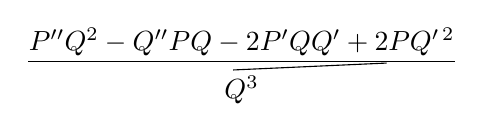
\begin{tikzpicture}
\node[inner sep=0pt,anchor=south west] (num) at (0,0)
 {$P''Q^2-Q''PQ-\unsure{2}P'QQ'+2PQ'^{\,2}$};
\path (num.south west)--(num.south east) coordinate[pos=0.48] (partialstart);
\path (num.south west)--(num.south east) coordinate[pos=0.84] (partialend);
\draw ([yshift=-2pt]num.south west)--([yshift=-2pt]num.south east);
\draw ([yshift=-5pt]partialstart)--([yshift=-2.5pt]partialend);
\node[inner sep=0pt,anchor=north,yshift=-7pt] at (num.south) {$Q^3$};
\end{tikzpicture}}
% The small quotient's fraction rule turns back at its right end; no arrow meaning is assigned.
\figure{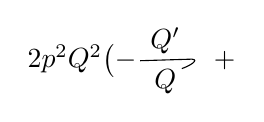
\begin{tikzpicture}
\node[inner sep=0pt,anchor=base west] (prefix) at (0,0) {$2p^2Q^2\bigl(-$};
\node[inner sep=0pt,anchor=south] at ([xshift=0.36cm,yshift=0.08cm]prefix.east) {$Q'$};
\node[inner sep=0pt,anchor=north] at ([xshift=0.36cm,yshift=-0.10cm]prefix.east) {$Q$};
\draw ([xshift=0.04cm]prefix.east)--([xshift=0.70cm,yshift=0.02cm]prefix.east)
 .. controls ([xshift=0.80cm,yshift=0.01cm]prefix.east) and ([xshift=0.66cm,yshift=-0.07cm]prefix.east)
 .. ([xshift=0.57cm,yshift=-0.10cm]prefix.east);
\node[inner sep=0pt,anchor=west] at ([xshift=0.97cm]prefix.east) {$+$};
\end{tikzpicture}}

% Opposite-direction writing, read after a half-turn. Two long diagonals cancel this layer.
\[
\deleted{\det\begin{pmatrix}a\deleted{\unsure{d|b}}&c\\b&d\end{pmatrix}-ad-bc\quad\text{inversible}}
\]
\[
\deleted{\begin{array}{c@{}l}
\delta(e_1 e_{d-2})&=-e_1\delta(e_{d-2})=-e_1e_{d-3}\deleted{=e_d}\\
\rotatebox{90}{$=$}&\\
\delta(a\eta)&=a\delta\eta=a\alpha e_{d-2}+a\beta f_{d-2}
\end{array}}
\]
\[
\deleted{\begin{array}{c@{}l}
\delta(e_1 f_{d-2})&=-\deleted{f}e_1\cdot f_{d-3}\\
\rotatebox{90}{$=$}&\\
b\alpha e_{d-2}+b\beta f_{d-2}&
\end{array}}
\]
\[
\deleted{\begin{array}{c@{}l}
\delta(f_1 e_{d-2})&=\delta(f_1)e_{d-2}-f_1\delta(e_{d-2})=e_{d-2}-f_1e_{d-3}\\
\rotatebox{90}{$=$}&\\
\delta(c\eta)&=c\delta\eta=c\alpha e_{d-2}+c\beta f_{d-2}
\end{array}}
\]
\deleted{etc}

% Detached dot at full-scan x=965--973, y=598--607, below and left of On after rotation.
% Its hand, layer, role, and cancellation state are unresolved; no relation to the formula is assigned.
\(\underset{\unsure{\text{.}}}{\phantom{\text{On}}}\)\deleted{On en tire $e_1e_{d-3}$, $\deleted{f}e_1f_{d-3}$\unsure{,} $f_1e_{d-3}$, $f_1f_{d-3}$ comme comb. lin des $e_{d-1}$ et $f_{d-2}$, à coeff entiers fonctions de $\alpha,\beta$, $a,b,c,d$}

\[
\deleted{\begin{array}{c@{}l}
\delta(e_1x_i)&=-e_1\delta(x_i)=-e_1\deleted{\unsure{\delta}}x_{i-1}\qquad 2\leq i\leq{}\\
\rotatebox{90}{$=$}&\\
\delta(\deleted{\unsure{S}}s e_{i+1}+t f_{i+1})&=s e_i+t f_i
\end{array}}
\]
% archive sheet number: 5

\scanpage{7}
\deleted{\illegible{1}} Soit $a\in\mathbb N^*,b\in\mathbb N^*,c\in\mathbb N^*,\ q\in\mathbb N^*$ \quad $q$ nombre premier $(q\ne1)$

On suppose que $a\mathrel{\underset{1}{\smile}}b$, $a\mathrel{\underset{1}{\smile}}c$, $b\mathrel{\underset{1}{\smile}}c$ (premiers entre eux deux à deux)
\inserted{et $a^q+b^q=c^q$}

On a $c>a$ et $c>b$ car $a\in\mathbb N^*$ et $b\in\mathbb N^*$

On pose $c=a+b'=b+a'$ avec $b'\in\mathbb N^*$ et $a'\in\mathbb N^*$
\[
\begin{aligned}
\text{alors}\qquad a^q+b^q=c^q&=(a+b')^q=\sum_{i=0}^{q}C_q^i\,a^i b'^{\,q-i}\qquad\text{(Newton)}\\
 &=b'^{\,q}+\sum_{i=1}^{q-1}C_q^i\,a^i b'^{\,q-i}+a^q\qquad(\text{car }q\geqslant2)
\end{aligned}
\]
\[
\text{donc}\qquad b^q=\sum_{i=1}^{q-1}C_q^i\,a^i b'^{\,q-i}+b'^{\,q}\tag*{(1)}
\]
la puissance de $b'$ n'étant jamais nulle on peut mettre $b'$ en facteur dans le second membre de (1), donc $b'\mid b^q$ ($b'$ divise $b^q$)

Soit $p$ un nombre premier % The phrase is visibly drawn once by rlap. The phantom preserves its deletion
% annotation and text dimensions without adding the generic horizontal rule.
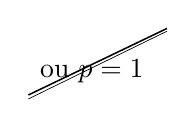
\begin{tikzpicture}[baseline=(cancelled.base)]
\node[inner sep=0pt,outer sep=0pt] (cancelled)
 {\rlap{ou $p=1$}\phantom{\deleted{ou $p=1$}}};
\draw[line width=.55pt] ([xshift=-1.5mm,yshift=-1.5mm]cancelled.south west) -- ([xshift=3mm,yshift=4mm]cancelled.north east);
\draw[line width=.25pt] ([xshift=-1.5mm,yshift=-2mm]cancelled.south west) -- ([xshift=3mm,yshift=3.65mm]cancelled.north east);
\end{tikzpicture}
 et tel que : $p\mid b'$ donc $p\mid b$. Soit $\alpha\in\mathbb N^*$ et $\alpha'\in\mathbb N^*$ tels que
\[
\begin{aligned}
 &p^{\alpha'}\mid b'\quad\text{et}\quad p^{\alpha'+1}\nmid b'\\
 \text{et}\quad &p^\alpha\mid b\quad\text{et}\quad p^{\alpha+1}\nmid b
\end{aligned}
\]
\margin{$\unsure{a|\alpha}$ \unsure{n'exist|n'existe} pas si on avait $p=1$}
On a $\alpha'\leqslant q\alpha$ car $b'\mid b^q$

\[
\begin{aligned}
(1)\ \Longrightarrow\quad&p^{q\alpha}\mid\sum_{i=1}^{q-1}C_q^i\,a^i b'^{\,q-i}+b'^{\,q}\\
\Longrightarrow\quad&p^{q\alpha}\mid b'\left(\sum_{i=1}^{q-1}C_q^i\,a^i b'^{\,q-i-1}+b'^{\,q-1}\right)\qquad(\text{car }q\geqslant2)
\end{aligned}
\]
posons $b'=p^{\alpha'}b''$ donc $b''\mathrel{\underset{1}{\smile}}p$ (propriété de $\alpha'$)
\[
\begin{aligned}
\Longrightarrow\quad&p^{q\alpha}\mid p^{\alpha'}b''\left(\sum_{i=1}^{q-1}C_q^i\,a^i b'^{\,q-i-1}+b'^{\,q-1}\right)\\
\Longrightarrow\quad&p^{q\alpha-\alpha'}\mid b''\left(\sum_{i=1}^{q-1}C_q^i\,a^i b'^{\,q-i-1}+b'^{\,q-1}\right)\quad\text{car }q\alpha\geqslant\alpha'\\
\Longrightarrow\quad&p^{q\alpha-\alpha'}\mid\sum_{i=1}^{q-1}C_q^i\,a^i b'^{\,q-i-1}+b'^{\,q-1}\quad\text{car }b''\mathrel{\underset{1}{\smile}}p
\end{aligned}
\]
% archive sheet number: 6

\scanpage{8}
% Upper-right mottled trace: visible patches only; no character, hand or role assigned.
\margin{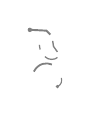
\begin{tikzpicture}[x=1cm,y=1cm]
\draw[gray,line width=.7pt] (.10,.84) -- (.29,.83) -- (.34,.78);
\fill[gray] (.08,.84) circle(.028cm);
\draw[gray,line width=.5pt] (.37,.70) -- (.38,.63) -- (.43,.56);
\draw[gray,line width=.45pt] (.20,.65) -- (.21,.59);
\draw[gray,line width=.45pt] (.27,.50) .. controls(.32,.45) and(.40,.46) .. (.43,.49);
\draw[gray,line width=.65pt] (.13,.31) .. controls(.19,.42) and(.29,.43) .. (.36,.40);
\fill[gray] (.43,.12) circle(.023cm);
\draw[gray,line width=.4pt] (.43,.12) .. controls(.48,.14) and(.49,.19) .. (.48,.23);
\end{tikzpicture}}
Supposons que $q\alpha-\alpha'\ne0$ alors
\[
\begin{aligned}
(1)\ \Longrightarrow\quad &p\mid\sum_{i=1}^{q-1}C_q^i\,a^i b'^{\,q-i-1}+b'^{\,q-1}\\
\Longrightarrow\quad &p\mid q\,a^{q-1}\qquad\text{Car }p\mid b'\ \text{et pour }i\ne q-1\quad q-i-1\deleted{\ne0}>0
\end{aligned}
\]
or $p\mid b'$ et $b'\mid b^q$ donc $b'\mathrel{\underset{1}{\smile}}a$ donc $p\mathrel{\underset{1}{\smile}}a$

\deleted{donc si $\unsure{p\ne1|p\ne q}$}
\[
(1)\ \Longrightarrow\quad p\mid q\qquad\text{donc }\deleted{p=1\ \text{ou }}p=q\quad(\text{si }q\alpha-\alpha'\ne0)
\]
Donc si $p\ne q$ \quad
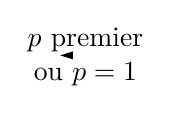
\begin{tikzpicture}[baseline=(p.base)]
\node[inner sep=0pt] (p) at (0,0) {$p$ premier};
\node[inner sep=0pt,anchor=north] at (0,-.28) {\inserted{ou $p=1$}};
% Small dark triangular mark above the addition; its guiding function is uncertain.
\fill (-.32,-.20) -- (-.16,-.15) -- (-.16,-.25) -- cycle;
\end{tikzpicture}
et $p\mid b'$ alors $\alpha'=q\alpha$
\begin{flushright}
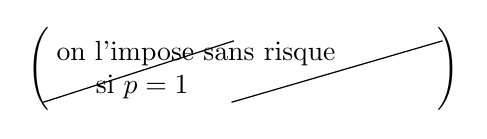
\begin{tikzpicture}[baseline=(u.base)]
\node[inner sep=0pt,anchor=west] (u) at (.22,0)
 {\rlap{on l'impose sans risque}\phantom{\deleted{on l'impose sans risque}}};
\node[inner sep=0pt,anchor=west] (v) at (.72,-.42)
 {\rlap{si $p=1$}\phantom{\deleted{si $p=1$}}};
\node[inner sep=0pt] at (0,-.20)
 {\rlap{$\Bigg($}\phantom{\deleted{$\Bigg($}}};
\node[inner sep=0pt] at (5.2,-.20)
 {\rlap{$\Bigg)$}\phantom{\deleted{$\Bigg)$}}};
% Two separate oblique cancellations over the two-line parenthesis.
\draw[line width=.45pt] (.06,-.62) -- (2.48,.16);
\draw[line width=.45pt] (2.45,-.62) -- (5.13,.16);
\end{tikzpicture}
\end{flushright}

Donc $\exists\,b_0\in\mathbb N^*$ et $\exists\,\gamma\in\mathbb N$ tel que $b'=q^\gamma b_0^q$ \margin{$q\nmid b_0$}

de plus $b_0\mid b$ et si $b=b_0 b''$ alors $b_0\mathrel{\underset{1}{\smile}}b''$ ?

De même $\exists\,a_0\in\mathbb N^*$ et $\exists\,\unsure{\zeta|\delta}\in\mathbb N$ tel que $a'=q^\zeta a_0^q$ avec $a_0\mid a$ et si $\overset{\unsure{\cdot|\prime}}{a}=a_0a''$ alors $a_0\mathrel{\underset{1}{\smile}}a''$ ?

or $a\mathrel{\underset{1}{\smile}}b\Longrightarrow a_{\deleted{\unsure{0}}}'\mathrel{\underset{1}{\smile}}b'\Longrightarrow\zeta\times\gamma=0$ (et aussi $a_0\mathrel{\underset{1}{\smile}}b_0$)

Je suppose désormais que $\zeta=0$ donc $a'=a_0^q$

\figure{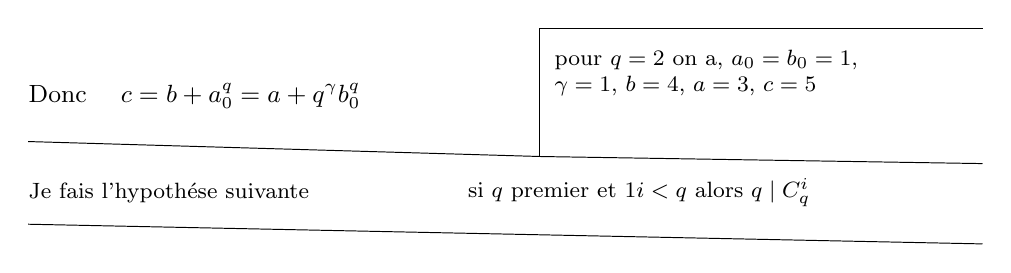
\begin{tikzpicture}[x=1cm,y=1cm]
\node[anchor=west,inner sep=0pt,font=\small] at (0,.80)
 {Donc \quad $c=b+a_0^q=a+q^\gamma b_0^q$};
\node[anchor=north west,inner sep=0pt,font=\footnotesize] at (6.68,1.43)
 {\begin{tabular}{@{}l@{}}
 pour $q=2$ on a, $a_0=b_0=1$,\\
 $\gamma=1$, $b=4$, $a=3$, $c=5$
 \end{tabular}};
% Open right border; the left edge meets the shared long upper rule.
\draw[line width=.35pt] (12.12,1.66) -- (6.50,1.66) -- (6.50,.03);
\draw[line width=.35pt] (0,.22) -- (6.50,.03) -- (12.12,-.06);
\node[anchor=west,inner sep=0pt,font=\footnotesize] at (0,-.43)
 {Je fais l'hypothése suivante};
\node[anchor=west,inner sep=0pt,font=\footnotesize] at (5.58,-.43)
 {si $q$ premier et $1\leqslant i<q$ alors $q\mid C_q^i$};
\draw[line width=.35pt] (0,-.83) -- (12.12,-1.08);
\end{tikzpicture}}
alors Si $q\geqslant3$ et $q\alpha-\alpha'\geqslant2$ \deleted{\unsure{alors}} on a \inserted{$p=q,\ {\unsure{a|\alpha}}'=\gamma$}
\[
\begin{aligned}
(1)\ \Longrightarrow\quad
 &\deleted{\unsure{p^{2}|p}}q^2\mid q\,a^{q-1}\quad
 
\begin{tikzpicture}[baseline=(d.base)]
 \node[inner sep=0pt] (d) at (0,0)
  {\rlap{ou $p=1$}\phantom{\deleted{ou $p=1$}}};
 \draw[line width=.45pt] (d.west) -- (d.east)
  .. controls +(0.22,-.04) and +(0.22,-.06) ..
  ([yshift=-2pt]d.east) -- ([yshift=-2pt]d.west);
 \end{tikzpicture}
\quad
% Faint residual strokes and points in the interline gap; no character is supplied.
\begin{tikzpicture}[baseline=-.05cm,x=1cm,y=1cm]
\draw[gray,line width=.35pt] (0,.12) .. controls (.10,.02) and (.18,-.02) .. (.31,.02);
\draw[gray,line width=.35pt] (.21,.13) -- (.27,.10);
\draw[gray,line width=.35pt] (.34,.02) .. controls (.40,.17) and (.42,.26) .. (.52,.24);
\draw[gray,line width=.35pt] (.49,.15) -- (.64,.14);
\fill[gray] (.58,.31) circle (.5pt);
\fill[gray] (.64,.04) circle (.45pt);
\fill[gray] (.69,-.02) circle (.45pt);
\end{tikzpicture}\\[.8ex]
\Longrightarrow\quad
 &q\mid a^{q-1}\quad
 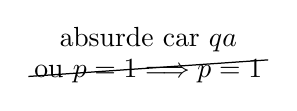
\begin{tikzpicture}[baseline=(d.base)]
 \node[inner sep=0pt] (d) at (0,0)
  {\rlap{ou $p=1\Longrightarrow p=1$}\phantom{\deleted{ou $p=1\Longrightarrow p=1$}}};
 \draw[line width=.45pt] ([xshift=-2pt,yshift=-2pt]d.west)
  -- ([xshift=2pt,yshift=4pt]d.east);
 \node[inner sep=0pt,anchor=south] at (0,.23)
  {\inserted{absurde car $q\nmid a$}};
 \end{tikzpicture}
\end{aligned}
\]
Donc $\gamma=0$ ou $\gamma=$
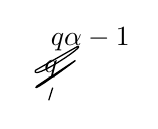
\begin{tikzpicture}[baseline=(q.base)]
\node[inner sep=0pt] (q) at (0,0)
 {\rlap{$q$}\phantom{\deleted{$q$}}};
% The live entry is physically raised above and to the right of the cancelled q.
\node[inner sep=0pt,anchor=south west] at (-.01,.22) {$q\alpha-1$};
\draw[line width=.45pt] (-.20,-.02) -- (.33,.28)
 .. controls (.48,.32) and (-.26,-.17) .. (-.20,-.02);
\draw[line width=.45pt] (-.18,-.22) -- (.30,.10)
 .. controls (.39,.16) and (-.29,-.34) .. (-.18,-.22);
\draw[line width=.45pt] (.02,-.24) -- (-.03,-.40);
\end{tikzpicture}
(sous réserve que l'hypothése est vraie)%
\margin{\begin{tikzpicture}[baseline=(n.base)]
\node[inner sep=0pt,text width=.85\marginparwidth] (n)
 {C'est peut-être interessant car ici $2$ est mis à part dans
 \(\mathord{\overset{\scriptscriptstyle\unsure{/}}{\vphantom{l}}}\)l'ensemble des nombres premiers};
% Small detached rising stroke before l'ensemble: role and hand unresolved.
% Return arrow rises at the right from the final parenthesis toward this note.
\fill ([xshift=.07cm,yshift=-.47cm]n.south east) circle(.022cm);
\draw ([xshift=.15cm,yshift=-.47cm]n.south east) -- ([xshift=.31cm,yshift=-.47cm]n.south east)
 -- ([xshift=.35cm,yshift=-.16cm]n.north east)
 .. controls([xshift=.35cm,yshift=-.03cm]n.north east) and([xshift=.19cm,yshift=-.01cm]n.north east)
 .. ([xshift=.06cm,yshift=.01cm]n.north east);
\draw ([xshift=.19cm,yshift=.14cm]n.north east) .. controls([xshift=.00cm,yshift=.04cm]n.north east) and([xshift=-.01cm,yshift=-.06cm]n.north east) .. ([xshift=.15cm,yshift=-.10cm]n.north east);
\end{tikzpicture}}
% archive sheet number: 7

\scanpage{10}
% Consolidated by root from three independent readings and seventeen adjudication crops.
% crop-candidate: scan 10
\figure{%
\begin{tikzpicture}[x=.0056cm,y=-.0056cm,line cap=round,line join=round,line width=.57pt,
 every node/.style={font=\scriptsize,inner sep=1pt}]
% Upper row. Coordinates follow the scans, with y increasing toward the foot.
\draw (118,180) .. controls (96,175) and (65,165) .. (63,146) .. controls (60,125) and (74,98) .. (94,68) .. controls (114,54) and (139,53) .. (158,62) .. controls (185,75) and (200,102) .. (186,137) .. controls (174,168) and (147,184) .. (118,180) -- cycle;
\draw (80,83) .. controls (88,71) and (96,67) .. (99,65);
\draw (136,55) .. controls (127,87) and (124,146) .. (117,181);
\draw (318,164) .. controls (303,149) and (280,133) .. (288,110) .. controls (294,84) and (305,65) .. (324,65) .. controls (344,61) and (369,61) .. (385,78) .. controls (402,97) and (402,127) .. (387,146) .. controls (369,166) and (333,176) .. (318,164) -- cycle;
\draw (304,85)--(313,65) (292,83) .. controls (303,69) and (310,78) .. (316,72);
\draw (359,63) .. controls (347,100) and (337,144) .. (319,163);
\draw (386,75) .. controls (376,99) and (355,139) .. (359,165);
\draw (528,88) .. controls (548,68) and (579,74) .. (590,94) .. controls (606,122) and (591,152) .. (572,164) .. controls (549,174) and (523,169) .. (512,155) .. controls (495,128) and (504,101) .. (528,88) -- cycle;
\draw (505,107) .. controls (512,94) and (526,94) .. (530,85);
\draw (527,88) -- (544,125) -- (563,157);
\draw (512,158) -- (544,125) -- (579,82);
\fill (545,125) circle[radius=7.5];
\node at (568,39) {OK};
\draw (714,165) .. controls (692,138) and (707,102) .. (741,82) .. controls (763,71) and (805,69) .. (824,85) .. controls (845,101) and (838,140) .. (811,169) .. controls (783,190) and (740,190) .. (714,165) -- cycle;
\draw (750,82) .. controls (741,112) and (733,154) .. (716,171);
\draw (789,74) .. controls (771,116) and (760,159) .. (758,188);
\draw (821,83) .. controls (812,113) and (798,150) .. (809,171);
\draw (774,82) -- (788,74);
\draw (877,167) .. controls (874,143) and (884,111) .. (899,102) .. controls (914,94) and (943,93) .. (957,104) .. controls (971,119) and (978,145) .. (968,163) .. controls (951,183) and (921,193) .. (898,188) .. controls (882,184) and (875,177) .. (877,167) -- cycle;
\draw (899,101) .. controls (909,128) and (902,148) .. (877,166);
\draw (934,99) .. controls (946,117) and (947,134) .. (977,137);
\draw (898,186) .. controls (925,163) and (946,151) .. (968,162);
\draw (925,98)--(927,104) (934,98)--(940,106);
\draw (1007,168) .. controls (1007,137) and (1016,107) .. (1031,102) .. controls (1052,96) and (1065,106) .. (1066,128) .. controls (1065,157) and (1048,186) .. (1027,195) .. controls (1016,201) and (1009,184) .. (1007,168) -- cycle;
\draw (1015,118) -- (1031,130) -- (1063,132) (1008,170) -- (1032,129) -- (1057,103);
\draw (1015,194) .. controls (1031,167) and (1054,156) .. (1054,176);
\fill (1033,130) circle[radius=5.3];
\draw (1038,111)--(1055,103);
\draw (1089,170) .. controls (1094,140) and (1114,106) .. (1137,93) .. controls (1161,77) and (1199,88) .. (1222,101) .. controls (1246,124) and (1228,161) .. (1207,184) .. controls (1180,207) and (1144,214) .. (1121,202) .. controls (1102,193) and (1091,184) .. (1089,170) -- cycle;
\draw (1086,171) -- (1137,135) -- (1167,113) -- (1196,92);
\draw (1119,103) -- (1138,135) .. controls (1151,149) and (1170,178) .. (1184,195);
\draw (1156,86) .. controls (1161,103) and (1168,122) .. (1179,137) .. controls (1195,152) and (1201,165) .. (1217,172);
\draw[line width=3pt] (1138,135) -- (1167,113);
\node at (1153,55) {OK};
\draw (1306,198) .. controls (1298,178) and (1312,140) .. (1333,113) .. controls (1351,93) and (1383,82) .. (1400,89) .. controls (1420,98) and (1435,120) .. (1430,147) .. controls (1413,188) and (1379,216) .. (1344,216) .. controls (1326,214) and (1312,207) .. (1306,198) -- cycle;
\draw (1317,195)--(1397,89) (1328,115)--(1425,174) (1297,172) .. controls (1340,167) and (1385,161) .. (1436,139);
\fill (1338,166)--(1363,135)--(1394,153)--cycle;
\draw[line width=2pt] (1376,90) .. controls (1385,86) and (1397,86) .. (1404,94);
\node at (1376,52) {OK};
\draw (1490,75) .. controls (1477,75) and (1450,148) .. (1446,194) .. controls (1442,229) and (1454,246) .. (1486,240);
\node at (1495,165) {ou};
\draw (1554,177) .. controls (1552,150) and (1562,112) .. (1579,106) .. controls (1599,99) and (1624,111) .. (1633,135) .. controls (1642,163) and (1621,194) .. (1600,205) .. controls (1579,218) and (1555,209) .. (1554,177) -- cycle;
\draw (1566,129) .. controls (1578,149) and (1590,162) .. (1618,175);
\draw (1583,104) .. controls (1582,132) and (1587,174) .. (1597,205);
\draw (1568,206)--(1613,107);
\draw (1567,184) .. controls (1567,196) and (1567,206) .. (1571,209);
\draw[line width=1pt] (1592,178) .. controls (1591,196) and (1590,217) .. (1587,238);
\fill (1587,159) circle[radius=6.5];
% Detached dark fragments beside the lower descending stroke; role uncertain.
\draw[line width=.7pt] (1596,174)--(1595,180) (1595,182)--(1593,187);
\fill (1584,198) circle[radius=1.2]; \fill (1598,226) circle[radius=1.2];
\draw[opacity=.45] (1548,116) .. controls (1562,103) and (1574,101) .. (1584,102);
\draw (1632,96) .. controls (1647,66) and (1657,114) .. (1649,157) .. controls (1641,212) and (1624,259) .. (1606,273);
\draw (759,202) .. controls (780,226) and (799,220) .. (828,212) .. controls (843,208) and (846,205) .. (846,217) .. controls (872,197) and (918,220) .. (949,210) -- (944,207);
\draw[line width=.55pt] (746,274) .. controls (747,244) and (777,229) .. (821,226) .. controls (863,222) and (910,214) .. (923,230) .. controls (940,253) and (888,293) .. (840,300) .. controls (787,310) and (751,304) .. (746,282) -- cycle;
\draw[line width=.7pt] (949,271) .. controls (947,245) and (987,240) .. (1015,235) .. controls (1044,226) and (1072,217) .. (1068,255) .. controls (1064,295) and (1053,303) .. (1014,305) .. controls (969,310) and (951,299) .. (949,271) -- cycle;
\node[inner sep=0pt] at (121,235) {\begin{minipage}{75pt}
\diagram{\begin{tikzcd}[ampersand replacement=\&,column sep=4pt,row sep=0pt,cells={nodes={inner sep=0pt,outer sep=0pt}}]
\bullet
\end{tikzcd}}
\end{minipage}};
\node[inner sep=0pt] at (325,236) {\begin{minipage}{75pt}
\diagram{\begin{tikzcd}[ampersand replacement=\&,column sep=4.7pt,row sep=0pt,cells={nodes={inner sep=0pt,outer sep=0pt}}]
\bullet \& \bullet
\end{tikzcd}}
\end{minipage}};
\node[inner sep=0pt] at (533,233) {\begin{minipage}{75pt}
\diagram{\begin{tikzcd}[ampersand replacement=\&,column sep=13pt,row sep=0pt,cells={nodes={inner sep=0pt,outer sep=0pt}}]
\vphantom{\bullet}\arrow[r,dash,line width=.65pt,start anchor=center,end anchor=center,shorten <=1pt,shorten >=1pt] \& \vphantom{\bullet}
\end{tikzcd}}
\end{minipage}};
\node[inner sep=0pt] at (852,253) {\begin{minipage}{75pt}
\diagram{\begin{tikzcd}[ampersand replacement=\&,column sep=8pt,row sep=0pt,cells={nodes={inner sep=0pt,outer sep=0pt}}]
\bullet \& \bullet \& \bullet
\end{tikzcd}}
\end{minipage}};
\node[inner sep=0pt] at (1009,262) {\begin{minipage}{75pt}
\diagram{\begin{tikzcd}[ampersand replacement=\&,column sep=4pt,row sep=0pt,cells={nodes={inner sep=0pt,outer sep=0pt}}]
\vphantom{\bullet}\arrow[r,dash,line width=.65pt,start anchor=center,end anchor=center,shorten <=1pt,shorten >=1pt] \&[5.2pt] \vphantom{\bullet} \&[-2pt] \bullet
\end{tikzcd}}
\end{minipage}};
\node[inner sep=0pt] at (1152,251) {\begin{minipage}{75pt}
\diagram{\begin{tikzcd}[ampersand replacement=\&,column sep=8.3pt,row sep=0pt,cells={nodes={inner sep=0pt,outer sep=0pt}}]
\bullet\arrow[r,dash,line width=.65pt,start anchor=center,end anchor=center,shorten <=1pt,shorten >=1pt] \& \unsure{\bullet|\circ}\arrow[r,dash,line width=.65pt,start anchor=center,end anchor=center,shorten <=2.7pt,shorten >=1pt] \& \bullet
\end{tikzcd}}
\end{minipage}};
\node[inner sep=0pt] at (1326,262) {\begin{minipage}{75pt}
\diagram{\begin{tikzcd}[ampersand replacement=\&,column sep=1.2pt,row sep=2.0pt,cells={nodes={inner sep=0pt,outer sep=0pt}}]
{} \& \bullet\arrow[dl,dash,line width=.65pt]\arrow[dr,dash,line width=.65pt] \& {}\\
\bullet\arrow[rr,dash,line width=.65pt] \& {} \& \bullet
\end{tikzcd}}
\end{minipage}};
% Two small, detached ink traces near the upper edge.
% Detached upper-edge marks: their hand and function remain undetermined.
\draw[opacity=.65,line width=.55pt] (1018,26) .. controls (1020,31) and (1023,32) .. (1025,27);
\draw[opacity=.65,line width=.55pt] (1037,29)--(1037,26) .. controls (1040,28) and (1043,28) .. (1046,25)--(1046,28);
% Middle row, left group.
\draw (116,390) .. controls (129,357) and (164,337) .. (200,327) .. controls (226,322) and (254,320) .. (272,326) .. controls (307,338) and (328,377) .. (326,413) .. controls (324,455) and (301,485) .. (265,500) .. controls (239,512) and (207,515) .. (184,510) .. controls (147,506) and (125,480) .. (116,455) .. controls (111,433) and (112,411) .. (116,390) -- cycle;
\draw (122,399) .. controls (122,392) and (126,388) .. (131,388);
\draw (154,353) .. controls (158,379) and (146,454) .. (128,472);
\draw (205,327) .. controls (203,354) and (205,404) .. (201,431) .. controls (197,465) and (193,491) .. (191,513);
\draw (270,324) .. controls (258,366) and (252,404) .. (253,433) .. controls (252,456) and (256,486) .. (263,501);
\draw (311,367) .. controls (296,393) and (290,441) .. (305,475);
\draw[opacity=.2] (192,503)--(195,556);
\draw (400,505) .. controls (378,492) and (374,467) .. (377,444) .. controls (382,413) and (403,377) .. (420,364) .. controls (441,342) and (462,334) .. (482,340) .. controls (514,337) and (544,366) .. (542,403) .. controls (543,444) and (508,491) .. (484,503) .. controls (462,516) and (428,521) .. (400,505) -- cycle;
\draw (419,365) .. controls (426,377) and (409,469) .. (400,503);
\draw (482,343) .. controls (461,390) and (451,446) .. (449,510);
\draw (517,356) .. controls (502,397) and (484,451) .. (481,501);
\draw[line width=1.6pt] (406,503) .. controls (423,481) and (428,504) .. (433,517);
\draw (433,512)--(434,519) (448,491)--(447,513) (456,346)--(482,340);
\draw (568,459) .. controls (563,432) and (570,399) .. (581,379) .. controls (594,358) and (612,345) .. (640,352) .. controls (665,358) and (685,385) .. (687,411) .. controls (693,446) and (680,490) .. (647,519) .. controls (636,523) and (624,523) .. (609,524) .. controls (590,517) and (571,499) .. (568,480) -- cycle;
\draw (598,359) .. controls (613,387) and (599,433) .. (567,459);
\draw (645,353) .. controls (653,386) and (676,407) .. (693,410);
\draw (570,480) .. controls (590,487) and (605,503) .. (610,524);
\draw[line width=1pt] (644,519) .. controls (647,504) and (665,473) .. (682,462);
\draw[line width=1.8pt] (684,395) .. controls (697,432) and (683,488) .. (651,516);
\draw (178,557) .. controls (177,574) and (221,577) .. (266,570) .. controls (311,564) and (361,554) .. (376,584) .. controls (378,560) and (416,560) .. (439,563) .. controls (497,573) and (539,558) .. (631,549);
\fill (733,427) circle[radius=2]; \fill (713,443) circle[radius=1.1];
% Middle row, right group.
\draw (778,444) .. controls (795,393) and (841,368) .. (889,367) .. controls (926,365) and (959,385) .. (977,414) .. controls (1001,449) and (966,489) .. (944,514) .. controls (923,544) and (901,563) .. (874,562) .. controls (842,564) and (800,553) .. (774,526) .. controls (774,509) and (771,472) .. (778,444) -- cycle;
\draw (772,446) .. controls (815,439) and (889,422) .. (947,388);
\draw (790,536) -- (854,425) -- (891,367);
\draw (778,464) .. controls (801,466) and (800,495) .. (777,509);
\draw (909,368) .. controls (910,392) and (925,388) .. (937,375);
\draw (774,517) .. controls (783,516) and (781,535) .. (791,536);
\fill (855,425) circle[radius=7.6];
\draw (990,500) .. controls (989,465) and (1002,432) .. (1026,409) .. controls (1047,386) and (1072,381) .. (1088,394) .. controls (1114,409) and (1110,444) .. (1104,473) .. controls (1098,508) and (1073,550) .. (1052,568) .. controls (1023,582) and (1009,571) .. (1000,548) .. controls (994,529) and (990,511) .. (990,500) -- cycle;
\draw (1021,412) .. controls (1043,438) and (1062,481) .. (1078,517);
\draw (998,534) .. controls (1023,505) and (1065,431) .. (1091,399);
\draw (998,456) .. controls (1018,463) and (1009,490) .. (991,501);
\draw (1015,570) .. controls (1034,544) and (1052,547) .. (1057,562);
\fill (1053,458) ellipse[x radius=6.8,y radius=9];
\draw (1133,512) .. controls (1136,476) and (1157,427) .. (1183,402) .. controls (1209,376) and (1248,380) .. (1268,395) .. controls (1296,420) and (1293,459) .. (1285,493) .. controls (1274,530) and (1241,562) .. (1208,571) .. controls (1171,582) and (1146,555) .. (1137,534) .. controls (1133,523) and (1132,516) .. (1133,512) -- cycle;
\draw (1172,411) -- (1207,472) .. controls (1222,498) and (1233,526) .. (1243,551);
\draw (1144,552) .. controls (1161,534) and (1218,450) .. (1266,395);
\draw (1155,453) .. controls (1175,478) and (1159,506) .. (1133,523);
\draw (1159,444) .. controls (1166,453) and (1181,440) .. (1171,428);
\fill (1207,472) circle[radius=7.3];
\draw (1285,514) .. controls (1291,476) and (1311,437) .. (1337,415) .. controls (1356,400) and (1381,409) .. (1391,423) .. controls (1417,463) and (1404,507) .. (1384,535) .. controls (1369,559) and (1349,583) .. (1327,588) .. controls (1306,591) and (1288,575) .. (1284,550) .. controls (1281,536) and (1282,525) .. (1285,514) -- cycle;
\draw (1315,444) -- (1342,491) -- (1368,559);
\draw (1290,564) .. controls (1307,552) and (1355,466) .. (1388,423);
\draw (1299,575) .. controls (1317,554) and (1335,524) .. (1347,555) -- (1353,570);
\draw (1312,585) .. controls (1328,561) and (1340,561) .. (1340,582);
\fill (1343,492) circle[radius=6.6];
\fill (1307,505) .. controls (1310,497) and (1314,496) .. (1318,483) .. controls (1324,477) and (1329,500) .. (1324,509) .. controls (1317,520) and (1305,515) .. (1307,505) -- cycle;
% Undetermined trace: pale intervals separate the darker parts of this upper extension.
\draw[opacity=.22] (1328,433) .. controls (1330,406) and (1335,357) .. (1341,329);
\draw[line width=.65pt] (1340,332)--(1339,339) (1338,343) .. controls (1336,351) and (1337,359) .. (1335,365);
\draw[line width=.55pt] (1333,382)--(1332,389) (1331,398)--(1330,403) (1329,411)--(1327,432);
\draw[line width=1.8pt] (1327,436) .. controls (1335,425) and (1340,416) .. (1349,418);
\draw (793,583) .. controls (822,621) and (923,616) .. (981,613) .. controls (1025,612) and (1060,623) .. (1079,622) .. controls (1090,628) and (1095,637) .. (1102,649) .. controls (1114,632) and (1127,626) .. (1138,621) .. controls (1220,627) and (1280,619) .. (1348,616) .. controls (1354,610) and (1360,601) .. (1364,592);
\draw (1004,605) .. controls (1015,626) and (1050,615) .. (1069,622) (1167,622) -- (1204,630);
\node[font=\bfseries\small] at (539,658) {?};
\node[inner sep=0pt] at (373,646) {\begin{minipage}{85pt}
\diagram{\begin{tikzcd}[ampersand replacement=\&,column sep=7pt,row sep=0pt,cells={nodes={inner sep=0pt,outer sep=0pt}}]
\bullet \& \bullet \& \bullet \& \bullet
\end{tikzcd}}
\end{minipage}};
\node[inner sep=0pt] at (848,648) {\begin{minipage}{85pt}
\diagram{\begin{tikzcd}[ampersand replacement=\&,column sep=11.1pt,row sep=0pt,cells={nodes={inner sep=0pt,outer sep=0pt}}]
\vphantom{\bullet}\arrow[r,dash,line width=.65pt,start anchor=center,end anchor=center,shorten <=1pt,shorten >=1pt] \& \vphantom{\bullet} \& \bullet \& \bullet
\end{tikzcd}}
\end{minipage}};
% Lower row.
\draw[opacity=.22,line width=.4pt] (1518,375) .. controls (1540,374) and (1561,405) .. (1524,401);
\fill[opacity=.75] (1566,580) circle[radius=1.25]; \fill[opacity=.65] (1561,587) circle[radius=1];
\node at (201,691) {OK};
\draw (123,811) .. controls (135,770) and (168,740) .. (208,726) .. controls (239,716) and (275,725) .. (304,749) .. controls (339,775) and (354,809) .. (350,840) .. controls (347,879) and (314,935) .. (279,960) .. controls (257,972) and (226,969) .. (198,968) .. controls (162,965) and (130,943) .. (121,913) .. controls (114,887) and (118,844) .. (123,811) -- cycle;
\draw (124,893) .. controls (149,863) and (184,800) .. (219,718);
\draw (125,813) -- (194,773) .. controls (223,757) and (257,743) .. (274,727);
\draw (198,968) -- (298,838) -- (340,790);
\draw (277,965) .. controls (283,927) and (291,876) .. (298,839) .. controls (303,812) and (307,781) .. (310,754);
\fill (194,773) circle[radius=7.5]; \fill (299,838) circle[radius=7];
\draw[opacity=.14] (252,825)--(256,825) (259,825)--(264,826) (267,826)--(271,826) (274,827)--(278,827);
\draw[opacity=.4] (278,827)--(293,828);
% State remains uncertain: diagonal cancellation | hatching. Only the visible diagonal paths are inked.
\node[inner sep=0pt,outer sep=0pt,anchor=center] at (548,820) {\unsure{\rlap{\hbox{\begin{tikzpicture}[x=.0056cm,y=-.0056cm,line cap=round,line join=round,line width=.57pt,color=black]
\path[use as bounding box] (450,714) rectangle (646,926);
\draw (460,830) .. controls (473,785) and (509,749) .. (541,731) .. controls (566,724) and (595,741) .. (613,754) .. controls (645,781) and (638,817) .. (626,842) .. controls (605,883) and (571,914) .. (538,917) .. controls (508,924) and (480,912) .. (462,889) .. controls (452,874) and (454,848) .. (460,830) -- cycle;
\draw (474,789) -- (612,754) (461,891) -- (547,729) (556,729) .. controls (578,778) and (605,805) .. (628,838);
% Repeated diagonal cancellation strokes in this disk.
\draw (535,717) .. controls (526,729) and (457,833) .. (461,835) .. controls (470,838) and (538,725) .. (537,729) .. controls (515,764) and (465,860) .. (470,865) .. controls (476,870) and (554,747) .. (565,747) .. controls (549,777) and (493,861) .. (493,865) .. controls (504,870) and (569,753) .. (585,751) .. controls (557,783) and (513,860) .. (518,866) .. controls (526,877) and (601,791) .. (614,798) .. controls (618,801) and (589,843) .. (563,892) .. controls (554,907) and (560,914) .. (572,923);
% Small pale descending trace and dark tip at the lower-left outline.
\draw[opacity=.16,line width=.4pt] (490,861) .. controls (488,885) and (490,901) .. (491,915);
\draw[line width=.55pt] (491,912)--(490,920);
\end{tikzpicture}}}\phantom{\deleted{\hbox{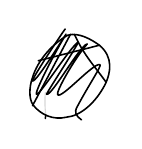
\begin{tikzpicture}[x=.0056cm,y=-.0056cm,line cap=round,line join=round,line width=.57pt,color=black]
\path[use as bounding box] (450,714) rectangle (646,926);
\draw (460,830) .. controls (473,785) and (509,749) .. (541,731) .. controls (566,724) and (595,741) .. (613,754) .. controls (645,781) and (638,817) .. (626,842) .. controls (605,883) and (571,914) .. (538,917) .. controls (508,924) and (480,912) .. (462,889) .. controls (452,874) and (454,848) .. (460,830) -- cycle;
\draw (474,789) -- (612,754) (461,891) -- (547,729) (556,729) .. controls (578,778) and (605,805) .. (628,838);
% Repeated diagonal cancellation strokes in this disk.
\draw (535,717) .. controls (526,729) and (457,833) .. (461,835) .. controls (470,838) and (538,725) .. (537,729) .. controls (515,764) and (465,860) .. (470,865) .. controls (476,870) and (554,747) .. (565,747) .. controls (549,777) and (493,861) .. (493,865) .. controls (504,870) and (569,753) .. (585,751) .. controls (557,783) and (513,860) .. (518,866) .. controls (526,877) and (601,791) .. (614,798) .. controls (618,801) and (589,843) .. (563,892) .. controls (554,907) and (560,914) .. (572,923);
% Small pale descending trace and dark tip at the lower-left outline.
\draw[opacity=.16,line width=.4pt] (490,861) .. controls (488,885) and (490,901) .. (491,915);
\draw[line width=.55pt] (491,912)--(490,920);
\end{tikzpicture}}}}}};
\draw (666,836) .. controls (669,808) and (686,789) .. (706,785) .. controls (725,782) and (746,786) .. (755,803) .. controls (773,824) and (771,857) .. (758,880) .. controls (746,903) and (728,917) .. (706,910) .. controls (683,903) and (660,871) .. (666,836) -- cycle;
\draw (707,786) -- (694,902) (747,789) .. controls (739,827) and (735,869) .. (729,906);
\draw (666,840)--(767,844);
\draw[line width=3.4pt] (699,838)--(737,842);
\draw (718,786) .. controls (715,814) and (733,813) .. (737,789);
\draw (797,850) .. controls (804,822) and (821,801) .. (839,798) .. controls (864,797) and (876,815) .. (881,839) .. controls (890,866) and (876,895) .. (860,910) .. controls (841,926) and (822,917) .. (809,905) .. controls (796,890) and (792,870) .. (797,850) -- cycle;
\draw (827,805) .. controls (823,843) and (819,878) .. (816,915);
\draw (862,805) .. controls (858,842) and (854,879) .. (852,914);
\draw (799,861)--(890,859); \draw[line width=2.8pt] (820,857)--(853,857);
\draw (874,818) .. controls (868,841) and (868,848) .. (885,850);
\draw (543,948) .. controls (573,976) and (607,963) .. (665,954) .. controls (706,949) and (731,945) .. (741,967) .. controls (744,947) and (789,945) .. (826,944) .. controls (864,943) and (881,941) .. (899,937) -- (898,931);
\node at (1156,724) {OK};
\draw (1004,849) .. controls (1005,815) and (1033,783) .. (1069,769) .. controls (1101,757) and (1134,762) .. (1150,787) .. controls (1172,815) and (1183,855) .. (1165,903) .. controls (1149,943) and (1125,964) .. (1109,969) .. controls (1072,976) and (1040,970) .. (1024,945) .. controls (1004,913) and (997,879) .. (1004,849) -- cycle;
\draw[opacity=.65] (1006,850) .. controls (1002,859) and (1003,869) .. (1009,874);
\draw (1012,924) .. controls (1029,875) and (1050,817) .. (1070,770);
\draw (1011,808) .. controls (1055,804) and (1125,796) .. (1156,788);
\draw (1101,764) .. controls (1110,780) and (1116,791) .. (1120,798) -- (1174,881);
\draw (1109,967) .. controls (1127,926) and (1154,855) .. (1172,823);
\draw[line width=2.7pt] (1056,802)--(1119,794);
\draw[line width=3.7pt] (1118,795)--(1158,853);
% Detached short dark trace below the broad segment; role and hand undetermined.
\draw[line width=.55pt] (1166,875)--(1165,879);
% Detached pale irregular patch; hand, origin and role remain undetermined.
\filldraw[fill opacity=.10,draw opacity=.16,line width=.3pt]
(1629,793) .. controls (1629,790) and (1631,788) .. (1635,788)
--(1636,786)--(1640,790)--(1645,792)
.. controls (1649,795) and (1648,799) .. (1646,802)
--(1643,803)--(1640,806)--(1637,808)--(1634,804)--(1630,804)
.. controls (1627,801) and (1627,797) .. (1629,793)--cycle;
% Two faint, angular lines at the foot, crossing the last graph and continuing at the right.
\draw[opacity=.55] (1010,975) .. controls (1027,995) and (1035,1030) .. (1044,1050) .. controls (1053,1074) and (1061,1090) .. (1075,1089);
\draw[line width=1.5pt] (1041,1036) .. controls (1052,1070) and (1060,1090) .. (1074,1088);
\draw[opacity=.16] (1073,1088) .. controls (1108,1087) and (1162,1076) .. (1214,1064) -- (1288,985);
\draw[opacity=.5] (1215,1073)--(1237,1044) (1246,1033)--(1261,1014) (1278,996)--(1289,982);
\draw[opacity=.22] (1345,934) .. controls (1353,954) and (1350,994) .. (1358,1009) -- (1372,1014);
\draw[line width=1.9pt] (1373,1014) .. controls (1390,1025) and (1430,1037) .. (1458,1048) -- (1484,1054) -- (1500,1036);
\draw[opacity=.5] (1487,1054)--(1581,957);
\draw[opacity=.23] (1568,905) .. controls (1572,924) and (1571,943) .. (1581,957);
\node[inner sep=0pt] at (222,1035) {\begin{minipage}{94pt}
\diagram{\begin{tikzcd}[ampersand replacement=\&,column sep=5.2pt,row sep=0pt,cells={nodes={inner sep=0pt,outer sep=0pt}}]
\unsure{\circ|\bullet}\arrow[r,dash,line width=.65pt,start anchor=center,end anchor=center,shorten <=1pt,shorten >=1pt] \& \circ \& \hspace{3.3pt} \& \bullet\arrow[r,dash,line width=.65pt,start anchor=center,end anchor=center,shorten <=1pt,shorten >=1pt] \& \bullet
\end{tikzcd}}
\end{minipage}};
\node[inner sep=0pt] at (563,1026) {\begin{minipage}{94pt}
\diagram{\begin{tikzcd}[ampersand replacement=\&,column sep=7pt,row sep=0pt,cells={nodes={inner sep=0pt,outer sep=0pt}}]
\unsure{\circ|\bullet}\arrow[r,dash,line width=.65pt,start anchor=center,end anchor=center,shorten <=1pt,shorten >=1pt] \& \bullet\arrow[r,dash,line width=.65pt,start anchor=center,end anchor=center,shorten <=2.7pt,shorten >=1pt] \& \bullet \& \bullet
\end{tikzcd}}
\end{minipage}};
\node[inner sep=0pt] at (1075,1032) {\begin{minipage}{94pt}
\diagram{\begin{tikzcd}[ampersand replacement=\&,column sep=9pt,row sep=0pt,cells={nodes={inner sep=0pt,outer sep=0pt}}]
\unsure{\bullet|\circ}\arrow[r,dash,line width=.65pt,start anchor=center,end anchor=center,shorten <=1pt,shorten >=1pt] \& \bullet\arrow[r,dash,line width=.65pt,start anchor=center,end anchor=center,shorten <=1pt,shorten >=1pt] \& \bullet\arrow[r,dash,line width=.65pt,start anchor=center,end anchor=center,shorten <=1pt,shorten >=1pt] \& \bullet
\end{tikzcd}}
\end{minipage}};

% Hook projecting above/right of the uncertain middle vertex under upper disk 7.
\draw[line width=.65pt] (1153,251) .. controls (1154,245) and (1159,246) .. (1163,252);
% Tiny detached spot just above the outer lower arch in the last middle disk.
\fill (1314,543) circle[radius=1.4];
% Pale detached marks; hand, purpose, and surface origin remain undetermined.
% Above upper disk4 the short course is supported; its faint lower continuation is unresolved.
\draw[opacity=.14,line width=.4pt] (416,241) .. controls (425,250) and (426,260) .. (421,266) .. controls (416,274) and (410,275) .. (403,275);
\draw[opacity=.16,line width=.4pt] (784,42) .. controls (784,49) and (785,55) .. (787,62);
\draw[opacity=.4,line width=.4pt] (786,56)--(786,59);
\draw[opacity=.16,line width=.35pt] (369,743) .. controls (379,751) and (390,762) .. (405,778) -- (415,786);
\draw[opacity=.25,line width=.4pt] (377,751)--(384,758) (390,764)--(393,767);
\draw[opacity=.14,line width=.4pt] (1567,352) .. controls (1570,358) and (1576,360) .. (1580,362);
% Pale diagonal inside the right angular trace, with independently detached lower dash.
% Only the short supported course is reproduced; a farther upper continuation remains unresolved.
\node[anchor=north west,inner sep=0pt,outer sep=0pt] at (1438,978) {\unsure{\hbox{\begin{tikzpicture}[x=.0056cm,y=-.0056cm,line cap=round,color=black]
\path[use as bounding box] (1438,978) rectangle (1504,1039);
\draw[opacity=.13,line width=.4pt] (1444,1037) .. controls (1460,1018) and (1488,989) .. (1500,980);
\end{tikzpicture}}}};
\draw[opacity=.45,line width=.45pt] (1435,1084)--(1437,1093);
% Dark pieces and small detached marks around the upper-right angular-trace endpoint.
\draw[opacity=.75,line width=.45pt] (1568,908)--(1570,917);
\fill[opacity=.65] (1566,921) circle[radius=1.15];
\fill[opacity=.3] (1550,893) circle[radius=1.2];
\fill[opacity=.2] (1603,930) circle[radius=1.6];
\end{tikzpicture}}
% archive sheet number: 9

\scanpage{11}
\[
 \unsure{=|\Rightarrow}
\]
\[
 \begin{aligned}
 \mathbb P\left(
 \begin{tikzpicture}[x=.0043cm,y=-.0043cm,baseline={(0,82)},line cap=round,line join=round]
 \draw[line width=.5pt] (18,12) -- (59,76) (64,1) -- (23,78);
 \draw[line width=.5pt] (0,1) -- (30,3) (63,0) -- (76,1)
 (0,80) -- (26,78) (58,76) -- (78,77);
 \end{tikzpicture}\right)&\qquad
 P(X\times\unsure{Z|2})\overset{?}{\simeq}
 \operatorname{Hom}(\underset{\unsure{\cdot}}{\deleted{\unsure{e|\mathcal E}}Z}\times X,\mathscr E)\\
 &\qquad\mathrel{/\!/}\quad
 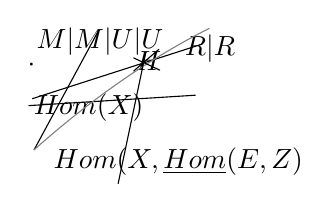
\begin{tikzpicture}[x=.011cm,y=-.011cm,baseline=(live.base),line cap=round,line join=round]
 % The cancellation paths are drawn explicitly. Invisible deleted copies retain the deletion annotation.
 \node[anchor=base west,inner sep=0] at (74,110)
 {\rlap{$\operatorname{Hom}(X)$}\phantom{$\deleted{\operatorname{Hom}(X)}$}};
 \node[inner sep=0] at (151,26)
 {$\unsure{\rlap{$M$}\phantom{\deleted{M}}|M|\rlap{$U$}\phantom{\deleted{U}}|U}$};
 \node[inner sep=0] at (207,48)
 {\rlap{$H$}\phantom{$\deleted{H}$}};
 \node[inner sep=0] at (278,34)
 {$\unsure{\rlap{$R$}\phantom{\deleted{R}}|R}$};
 \draw (69,100) -- (261,88);
 \draw (73,92) -- (269,29);
 \draw (75,151) -- (149,14);
 \draw[gray] (75,151) .. controls (120,111) and (191,54) .. (277,11);
 \draw (172,190) -- (204,38);
 \draw (190,60) -- (219,35) (190,45) -- (220,59);
 \node[inner sep=0] at (72,54) {$\unsure{\cdot}$};
 \node[anchor=base west,inner sep=0] (live) at (97,173)
 {$\operatorname{Hom}(X,\underline{\operatorname{Hom}}(\mathscr E,Z)$};
 \end{tikzpicture}\\
 \unsure{O|0}\subset\mathbb{P}(X)&\qquad
 \operatorname{Hom}(\mathscr E,\underline{\operatorname{Hom}}(X,Z))\\
 &\qquad\mathrel{/\!/}\\
 &\qquad P(\operatorname{Hom}(X,Z)
 \end{aligned}
\]
\figure{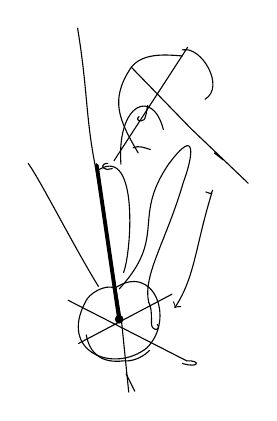
\begin{tikzpicture}[x=.011cm,y=-.011cm,line cap=round,line join=round]
\draw (63,1) .. controls (75,74) and (72,104) .. (84,163) -- (114,342) -- (122,421);
\draw[line width=1.4pt] (85,159) -- (111,337);
\draw (6,157) .. controls (22,180) and (57,250) .. (87,299);
\draw (64,365) -- (172,308) (52,315) -- (189,385);
\draw (106,301) .. controls (151,271) and (176,337) .. (143,370)
 .. controls (105,400) and (41,375) .. (72,317) .. controls (76,307) and (95,296) .. (106,301);
\fill (111,337) circle (5);
\draw (105,154) -- (190,23) (184,26) .. controls (206,21) and (234,69) .. (210,83)
 (125,46) -- (194,117) -- (260,180) (231,153) -- (221,145);
\draw (133,145) .. controls (110,106) and (100,83) .. (125,46) .. controls (139,28) and (169,32) .. (184,33);
\draw (113,158) .. controls (108,87) and (150,70) .. (162,118);
\draw (88,164) .. controls (134,137) and (125,261) .. (116,283);
\draw (111,302) .. controls (167,241) and (125,221) .. (168,158)
 .. controls (202,112) and (196,150) .. (185,179) .. controls (166,245) and (138,286) .. (145,317);
\draw[->] (218,191) .. controls (199,252) and (199,287) .. (175,324);
% Local small paths seen in the junction and disk crops; no letter or role assigned.
\draw (98,157) .. controls (90,157) and (90,163) .. (97,164) -- (103,163);
\draw (127,139) .. controls (134,136) and (140,139) .. (147,141);
\draw (144,90) .. controls (142,98) and (142,109) .. (136,108)
 .. controls (132,108) and (131,105) .. (134,103);
\draw (73,355) .. controls (77,377) and (91,388) .. (116,385)
 .. controls (128,386) and (139,380) .. (146,373);
\draw (189,385) .. controls (205,384) and (204,394) .. (184,388);
\draw (145,317) .. controls (151,329) and (146,344) .. (150,347)
 .. controls (156,352) and (158,345) .. (155,343);
\draw (119,400) -- (129,420);
\draw (211,190) -- (217,192) -- (219,188);
% crop-candidate: scan 11
\end{tikzpicture}}
\[
 \begin{aligned}
 \begin{tikzpicture}[baseline=(hom.base),line cap=round]
 \node[inner sep=0] (hom) at (0,0) {$\underline{\operatorname{Hom}}$};
 \node[inner sep=0] at (-.78,.12) {\unsure{\begin{tikzpicture}[x=.015cm,y=-.015cm]
 \draw[gray] (0,0) .. controls (3,3) and (6,5) .. (10,6);
 \draw (10,6) -- (12,6.5);
 \end{tikzpicture}}};
 \end{tikzpicture}(X,Y)&\subset P(X\times Y)\\
 \operatorname{Hom}(\begin{tikzpicture}[baseline=(z.base),line cap=round,line join=round]
 \node[inner sep=0] (z) at (0,0) {$\deleted{\unsure{t|1}}Z$};
 \node[inner sep=0] at (.17,.48) {\unsure{\begin{tikzpicture}[line cap=round,line join=round]
 \draw (0,0) -- (.08,.06) -- (.15,.03) -- (.23,.06) -- (.30,.04);
 \fill (.38,.04) circle (.012);
 \fill[gray] (.43,.03) circle (.009);
 \end{tikzpicture}}};
 \end{tikzpicture}\times X,Y)&\subset
 \underset{\text{\unsure{\begin{tikzpicture}[x=.014cm,y=-.014cm,baseline=0,line cap=round,line join=round]
 \draw (-13,0) -- (-8,1);
 \draw (-2,2) -- (0,-2) -- (3,1) -- (5,-1) -- (6,2);
 \draw (10,-1) -- (11,3);
 \end{tikzpicture}}}}{P}
 (\underset{\text{\unsure{\begin{tikzpicture}[x=.014cm,y=-.014cm,baseline=0,line cap=round]
 \fill (-8,0) circle (1.2);
 \fill[gray] (1,1) circle (1.4);
 \draw[gray] (6,2) -- (8,-1) (12,1) -- (13,-1) (15,0) -- (17,-2);
 \end{tikzpicture}}}}{Z}\times X\times Y)
 \end{aligned}
\]
\diagram{\begin{tikzcd}[ampersand replacement=\&,row sep=small,column sep=small,
 execute at end picture={
  % Retraced lower horizontal arrow shaft and extended upper head stroke.
  \draw[line width=.45pt] ([xshift=-4pt,yshift=-1pt]sxiU.west)
    .. controls ([xshift=-18pt,yshift=-5pt]sxiU.west) and ([xshift=15pt,yshift=-5pt]sxiV.east)
    .. ([xshift=4pt,yshift=-1pt]sxiV.east);
  \draw ([xshift=8pt,yshift=5pt]sxiV.east) -- ([xshift=11pt,yshift=9pt]sxiV.east);
  % Loop at the downward arrowhead, plus its two detached marks.
  \draw ([xshift=-5pt,yshift=9pt]sxiPX.north)
    .. controls ([xshift=-9pt,yshift=14pt]sxiPX.north) and ([xshift=-10pt,yshift=8pt]sxiPX.north)
    .. ([xshift=-4pt,yshift=6pt]sxiPX.north);
  \node[inner sep=0] at ([xshift=-12pt,yshift=14pt]sxiPX.north) {$\unsure{\cdot}$};
  \node[inner sep=0] at ([xshift=14pt,yshift=5pt]sxiPX.north) {$\unsure{\textcolor{gray}{\cdot}}$};
 }]
 \& {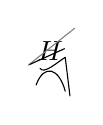
\begin{tikzpicture}[baseline=(h.base),line cap=round,line join=round]
 \node[inner sep=0] (h) at (0,0) {\rlap{$H$}\phantom{$\deleted{H}$}};
 \draw[gray] (-.28,-.18) -- (.31,.29);
 \draw (-.26,-.17) -- (.18,.03);
 \draw (-.13,-.22) .. controls (-.08,-.30) and (.09,-.14) .. (.19,-.08);
 \draw (.19,-.08) -- (.25,-.57);
 \draw (-.18,-.43) .. controls (-.08,-.16) and (.11,-.21) .. (.19,-.51);
 \end{tikzpicture}} \& \& \\
 \& {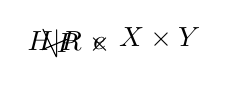
\begin{tikzpicture}[baseline=(prod.base),line cap=round,line join=round]
 \node[inner sep=0] at (-.12,0) {\rlap{$\unsure{H|R}$}\phantom{$\deleted{\unsure{H|R}}$}};
 \node[inner sep=0] (prod) at (.04,0) {$P$};
 \draw (-.27,.18) -- (-.10,-.17) (-.28,-.08) -- (.03,.05);
 \node[inner sep=0] at (.45,0) {\rlap{$e$}\phantom{$\deleted{e}$}};
 \node[inner sep=0] at (.45,-.02) {$\times$};
 \node[anchor=base west,inner sep=0] at (.69,-.04) {$X\times Y$};
 \end{tikzpicture}}
 \arrow[d,"{
\begin{tikzpicture}[baseline=(u.base),line cap=round,line join=round]
 \node[inner sep=0] (u) at (0,0)
 {\rlap{$\unsure{H|U}$}\phantom{$\deleted{\unsure{H|U}}$}};
 \draw (-.21,-.21) -- (.24,.36);
 \draw (.05,-.13) .. controls (-.03,-.45) and (.13,-.54) .. (.33,-.31);
 \end{tikzpicture}}"'] \& \&
 {\supset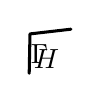
\begin{tikzpicture}[baseline=(g.base),line cap=round,line join=round]
 \node[inner sep=0] at (.09,-.04) {\rlap{$H$}\phantom{$\deleted{H}$}};
 \node[inner sep=0] (g) at (0,.03) {$\Gamma$};
 \draw[line width=1.1pt] (-.13,-.22) -- (-.12,.28) -- (.40,.34);
 \end{tikzpicture}}\arrow[dll] \\
 \& |[alias=sxiPX]| P\times X\arrow[dl] \& \& U\times_{\unsure{Y|V}}U\\
 {\begin{tikzpicture}[baseline=(p.base),line cap=round]
 \node[inner sep=0] (p) at (.29,-.25) {$P$};
 \node[inner sep=0] at (-1.03,.91) {$\unsure{\cdot}$};
 \draw[gray] (-1.11,.94) .. controls (-1.10,.92) and (-1.08,.91) .. (-1.07,.90);
 \draw (-.08,1.0) .. controls (-.06,.35) and (-.12,-.55) .. (-.09,-1.04);
 \draw (-.06,.48) .. controls (-.03,-.10) and (.02,-.67) .. (.08,-.92);
 \node[inner sep=0] at (.21,.03) {\unsure{\begin{tikzpicture}[x=.015cm,y=-.015cm,line cap=round]
 \draw[gray] (0,0) .. controls (3,-3) and (4,0) .. (3,3) -- (4,8);
 \end{tikzpicture}}};
 \end{tikzpicture}}
 \& |[alias=sxiV]| \unsure{V|W} \& \& |[alias=sxiU]| U\arrow[ll]\\
 \& \& {\begin{tikzpicture}[x=.011cm,y=-.011cm,baseline=(p.base),line cap=round]
 \node[inner sep=0,anchor=base] (p) at (0,0) {$P$};
 \draw (-42,-102) .. controls (-30,-94) and (-30,-78) .. (-22,-66);
 \draw[gray] (60,-113) -- (30,-59);
 \fill (30,-59) circle (1.2);
 \node[inner sep=0] at (2,21) {\unsure{\begin{tikzpicture}[x=.011cm,y=-.011cm,line cap=round]
 \draw[line width=.7pt] (-1,-13) .. controls (0,-4) and (1,5) .. (3,13);
 \fill (3,13) circle (1.2);
 \end{tikzpicture}}};
 \end{tikzpicture}} \&
\end{tikzcd}}
\figure{\begin{tikzpicture}[x=.011cm,y=-.011cm,line join=round,line cap=round]
% crop-candidate: scan 11
% The three bottom drawings were checked individually on the supplied halves.
\draw (13,425) -- (98,53);
\draw (98,46) -- (130,35) (139,32) -- (155,26) (164,23) -- (215,4);
\draw (215,4) -- (282,69);
\draw (282,76) -- (267,303) -- (145,352) -- (13,425);
\draw (215,4) -- (210,-3) (219,5) -- (218,-4);
\draw (13,425) -- (6,414) (267,303) -- (270,313);
\draw[line width=1.8pt] (216,8) -- (272,69) (278,226) -- (267,304) -- (147,351) -- (41,253);
\draw (209,4) .. controls (230,40) and (248,53) .. (272,68) (282,74) -- (219,0);
\draw (6,237) .. controls (47,191) and (63,184) .. (74,188)
 (3,214) -- (144,362) -- (178,405) (6,209) -- (159,358);
\draw (35,185) .. controls (-5,206) and (15,266) .. (48,309)
 .. controls (115,383) and (151,428) .. (171,406);
\draw[->] (46,199) .. controls (80,196) and (208,305) .. (184,407);
\draw (86,366) .. controls (86,389) and (188,345) .. (237,329);
\draw (319,271) -- (430,382) -- (549,389) -- (624,258) (319,271) -- (498,464) (535,454) -- (617,264);
\draw[line width=2pt] (325,275) -- (429,374) -- (556,384) -- (620,263);
\draw (319,268) -- (556,384) (361,299) -- (543,381);
\draw (501,486) .. controls (530,446) and (552,450) .. (570,357);
\draw (416,389) .. controls (421,396) and (430,396) .. (438,389);
\draw (562,388) -- (574,391) (564,398) -- (578,402);
\node[inner sep=0] at (523,276) {\unsure{\begin{tikzpicture}[x=.011cm,y=-.011cm,line cap=round]
\fill (0,0) circle (1.2); \draw[gray] (1,1) -- (3,2);
\end{tikzpicture}}};
\draw (627,259) -- (745,421);
\draw (640,291) .. controls (722,169) and (814,239) .. (883,324)
 .. controls (934,419) and (753,461) .. (678,394) .. controls (654,378) and (643,338) .. (648,316);
\draw (676,252) .. controls (710,302) and (679,351) .. (678,400)
 (705,230) .. controls (675,312) and (707,386) .. (709,416)
 (731,225) .. controls (722,312) and (765,383) .. (782,421);
\draw (783,244) -- (868,399) (815,250) .. controls (797,322) and (811,374) .. (850,416)
 (860,285) .. controls (847,342) and (824,363) .. (822,426);
\draw (684,318) -- (698,354) -- (685,337) -- (698,365)
 (811,316) -- (835,347) -- (812,328) -- (837,358) -- (813,342) -- (833,369);
\end{tikzpicture}}
% archive sheet number: 10

\scanpage{12}
% Consolidated scan012; all root crop decisions are recorded in the accompanying changes log.
% All source full-pixel coordinates and literal C contour blocks are retained.
% Editorial descriptions and alternatives appear only in comments.
\figure{\begin{tikzpicture}[x=0.0076cm,y=-0.0076cm,line join=round,line cap=round]
% C source path 01: literal block retained once.
\path[fill=black,even odd rule]
(505.5,23) -- (514,23.6) -- (529.4,34) -- (535.4,44) -- (538.4,56) -- (538.5,62) -- (536.5,67) -- (537.4,71) -- (533.6,75) -- (531.4,81)
 -- (528.7,83) -- (530,89.5) -- (528,90.4) -- (523,88.4) -- (523.3,86) -- (519,81.7) -- (515,82.7) -- (511.7,86) -- (509.7,93) -- (515,92.3)
 -- (520,88.6) -- (522.5,89) -- (522.5,90) -- (522.4,91) -- (517,94.4) -- (505,98.5) -- (496,96.4) -- (494,94.7) -- (492,96.4) -- (488.6,96)
 -- (487.7,94) -- (489.3,89) -- (483.6,76) -- (481.5,55) -- (484.3,42) -- (483.7,39) -- (486.6,34) -- (491,29.6) -- (502,23.6) -- cycle
(510,26.8) -- (506.7,29) -- (503,45.3) -- (508,46.1) -- (523.1,32) -- (518,28.6) -- cycle
(525,33.7) -- (508.7,50) -- (535,67.3) -- (536.5,58) -- (534.5,47) -- (529.3,38) -- cycle
(488,42.9) -- (486.7,44) -- (485.5,51) -- (484.7,63) -- (486,64.2) -- (495.3,57) -- (497.5,51) -- (495.4,48) -- cycle
(502,27.8) -- (492,37.3) -- (490,35.8) -- (488.7,37) -- (489.6,40) -- (497,45.3) -- (499.3,43) -- (503.3,31) -- cycle
(508,53.8) -- (500.7,57) -- (493.7,88) -- (497,93.3) -- (504,95.2) -- (506.3,93) -- (508.6,85) -- (513,79.6) -- (521,78.6) -- (527,82.3)
 -- (532.5,75) -- (532.3,72) -- (530,68.7) -- (526,71.4) -- (524.3,66) -- (521.4,63) -- cycle
(495,59.9) -- (485.7,70) -- (490,85.3) -- (491,85.3) -- (491.3,85) -- (492.3,82) -- (495.3,68) -- cycle
;
% C source path 02: literal block retained once.
\path[fill=black,even odd rule]
(318.5,47) -- (334,46.5) -- (343,47.6) -- (367,55.6) -- (391,69.6) -- (398,74.6) -- (409,85.5) -- (415.4,93) -- (423.4,106) -- (431.4,129)
 -- (431.7,135) -- (438,137.6) -- (439.4,140) -- (439.4,141) -- (439,141.4) -- (434,141.7) -- (433.7,142) -- (433.5,143) -- (435.5,154) -- (436.4,180)
 -- (435,187.2) -- (432.5,150) -- (431.3,143) -- (431,142.7) -- (430,142.5) -- (403,154.4) -- (387,158.7) -- (362,169.4) -- (340,176.7) -- (312,189.4)
 -- (294,192.7) -- (293.7,193) -- (293.7,194) -- (306,201.3) -- (327,210.3) -- (338,213.6) -- (371,229.3) -- (390,236.3) -- (397,237.6) -- (423,252.1)
 -- (430.3,222) -- (431.5,212) -- (430.6,191) -- (434,188.6) -- (439,188.7) -- (443.4,192) -- (443.5,193) -- (443.4,194) -- (443,194.4) -- (442,194.4)
 -- (440,191.7) -- (439,191.5) -- (438,191.5) -- (434.7,194) -- (434.4,217) -- (426.5,253) -- (428,255.3) -- (441,260.6) -- (441.4,263) -- (424.7,260)
 -- (417.4,285) -- (407.4,309) -- (399.4,323) -- (382.4,345) -- (372.7,353) -- (373.4,357) -- (369,363.4) -- (366.6,362) -- (366,357.9) -- (360,363.4)
 -- (350,369.4) -- (339,372.7) -- (336,375.4) -- (328,375.7) -- (320,377.5) -- (318,379.4) -- (311.6,379) -- (311.6,378) -- (312,377.5) -- (318,377.3)
 -- (318.3,377) -- (318.4,376) -- (318,375.7) -- (317,375.5) -- (298,378.5) -- (292,375.4) -- (277,377.4) -- (260,376.4) -- (242,371.4) -- (230,365.7)
 -- (226,365.4) -- (223,361.7) -- (215,357.4) -- (194.6,340) -- (175.6,318) -- (169.6,309) -- (161.6,293) -- (158.3,283) -- (151.6,272) -- (150.5,258)
 -- (152.5,250) -- (151.6,226) -- (153.3,223) -- (153.5,212) -- (155.5,201) -- (155.3,200) -- (155,199.7) -- (147,199.4) -- (146.6,197) -- (153,194.6)
 -- (156.3,195) -- (162.6,165) -- (165.6,154) -- (167.3,152) -- (168.6,144) -- (173.6,132) -- (179.3,123) -- (175.6,119) -- (177.5,116) -- (178,115.6)
 -- (179,115.6) -- (183,118.3) -- (197.5,99) -- (218,83.6) -- (235,73.6) -- (238,73.3) -- (256,63.6) -- (273,56.6) -- (299,50.3) -- (302,48.6) -- cycle
(326,49.8) -- (306,51.7) -- (288,55.7) -- (256,67.7) -- (237,76.7) -- (233.7,81) -- (231.4,88) -- (228.7,90) -- (224.7,97) -- (221.4,107)
 -- (206.7,138) -- (214,144.3) -- (219,142.6) -- (218.7,147) -- (226,153.3) -- (274,183.3) -- (288,189.5) -- (310,186.3) -- (332,175.6) -- (357,167.3)
 -- (390,153.6) -- (406,148.3) -- (429.3,137) -- (428.3,128) -- (426.6,126) -- (421.3,109) -- (416.3,100) -- (403.4,84) -- (381,67.7) -- (366,59.7)
 -- (343,51.7) -- cycle
(160,200.7) -- (158.4,219) -- (156.8,224) -- (157,233.3) -- (158,233.3) -- (158.3,233) -- (159.6,229) -- (168.3,216) -- (168.6,213) -- (174.3,202)
 -- (173,200.5) -- cycle
(182,125.7) -- (179.8,130) -- (180.4,133) -- (175.7,138) -- (167.7,161) -- (160.7,190) -- (161,196.3) -- (176,196.3) -- (178.3,194) -- (191.6,162)
 -- (201.3,143) -- (201.5,142) -- (201.3,141) -- (199.4,139) -- cycle
(225,83.7) -- (201,101.7) -- (185.7,120) -- (186.6,123) -- (202,135.3) -- (204.3,135) -- (210.6,120) -- (215.3,113) -- (223.6,90) -- (226.3,86)
 -- (226.5,85) -- (226.3,84) -- (226,83.7) -- cycle
(209,147.7) -- (205.7,151) -- (198,172.1) -- (200,171.4) -- (202.3,168) -- (206.6,158) -- (212.2,150) -- (211,147.7) -- (210,147.5) -- cycle
(215,151.7) -- (202.7,173) -- (200,182.3) -- (205.3,177) -- (207.6,172) -- (213.3,165) -- (214.6,161) -- (219.3,156) -- (218,152.5) -- cycle
(222,156.7) -- (215.7,167) -- (207.7,190) -- (208,193.3) -- (210.3,192) -- (228.3,161) -- (227,158.7) -- cycle
(231,161.8) -- (215.7,190) -- (216,194.1) -- (219.3,192) -- (219.5,191) -- (219.6,190) -- (235,170.6) -- (236,170.6) -- (236.4,171) -- (236.4,174)
 -- (226.7,189) -- (226,193.1) -- (230.4,193) -- (249.1,173) -- (247,170.7) -- cycle
(251,174.7) -- (239.7,189) -- (240,192.3) -- (242.4,192) -- (256.3,178) -- (255,175.7) -- cycle
(259,178.9) -- (256.4,185) -- (253.7,187) -- (251.7,191) -- (253,192.3) -- (261,190.3) -- (270.1,186) -- cycle
(273,187.7) -- (263.9,192) -- (271,192.3) -- (277.3,191) -- (275,187.7) -- (274,187.5) -- cycle
(279,194.7) -- (270,196.5) -- (246,195.5) -- (237,198.3) -- (233,196.5) -- (228,197.7) -- (224,200.5) -- (220,197.5) -- (216,198.5) -- (197,197.8)
 -- (178.7,200) -- (168.4,222) -- (158.7,237) -- (156.5,243) -- (155.7,265) -- (156.7,272) -- (161.4,278) -- (163.7,289) -- (172.7,307) -- (178,315.4)
 -- (199.6,340) -- (205,345.3) -- (225,359.3) -- (227.4,359) -- (242,343.6) -- (258,330.6) -- (270,323.6) -- (273,323.3) -- (280,319.6) -- (293,317.5)
 -- (317,320.6) -- (333,326.6) -- (343,331.6) -- (355,342.3) -- (370,351.3) -- (380,342.4) -- (401.3,313) -- (413.3,285) -- (421.3,258) -- (406,249.4)
 -- (397,242.7) -- (364,231.4) -- (336,217.7) -- (310,208.4) -- (291,197.7) -- cycle
(202,147.7) -- (183.7,189) -- (182,196.3) -- (200,195.3) -- (205.3,193) -- (205.6,188) -- (209,177.7) -- (208,177.7) -- (207.7,178) -- (199,192.4)
 -- (195.7,191) -- (197.2,185) -- (196,183.8) -- (192,191.4) -- (189.5,189) -- (190.6,182) -- (201.3,156) -- (203.3,149) -- cycle
(223,190.9) -- (222,193.3) -- (223,193.3) -- (223.3,193) -- cycle
(235,190.7) -- (235,193.1) -- (237.1,191) -- cycle
(250,187.9) -- (246.8,191) -- (248,192.2) -- (250.4,191) -- cycle
(285,322.7) -- (274,326.7) -- (255,337.7) -- (230.7,362) -- (239,366.3) -- (256,372.3) -- (272,374.5) -- (292,374.5) -- (305,371.6) -- (314,372.5)
 -- (321,370.5) -- (337,371.3) -- (351,365.3) -- (363.1,357) -- (363,354.6) -- (353.4,346) -- (332,331.7) -- (309,323.7) -- cycle
;
% C source path 03: literal block retained once.
\path[fill=black,even odd rule]
(732.5,91) -- (736,90.6) -- (740,95.5) -- (747,95.3) -- (753,93.6) -- (756,94.5) -- (769,93.5) -- (780,96.3) -- (779.6,92) -- (781,90.6)
 -- (786,96.2) -- (790,92.6) -- (791,92.5) -- (792,92.6) -- (794.4,97) -- (790,96.7) -- (788.7,99) -- (801,106.6) -- (815.4,123) -- (829.4,146)
 -- (833.4,156) -- (837.4,174) -- (839.4,197) -- (835.5,223) -- (837.3,233) -- (830.7,238) -- (821.4,261) -- (811.4,281) -- (799.4,301) -- (791,312.5)
 -- (774.7,328) -- (772,332.5) -- (766.8,336) -- (772.4,341) -- (772,343.4) -- (767,342.7) -- (764,345.3) -- (760,340.7) -- (752,344.7) -- (748,348.4)
 -- (734,354.4) -- (721,358.4) -- (710,359.7) -- (704,362.4) -- (698,362.4) -- (692,359.5) -- (683,360.5) -- (666,358.7) -- (662,359.7) -- (657.6,363)
 -- (652,372.4) -- (645,373.4) -- (644.6,371) -- (649.3,367) -- (649.6,364) -- (651.3,362) -- (650.1,359) -- (640,370.5) -- (638,370.5) -- (636.7,369)
 -- (637.6,367) -- (648.3,357) -- (641,355.4) -- (625.5,346) -- (605,324.5) -- (594.6,308) -- (588.6,295) -- (584.6,282) -- (583.5,274) -- (584.3,255)
 -- (579.6,250) -- (578.6,241) -- (584,237.6) -- (587,237.3) -- (590.3,234) -- (621.6,168) -- (630.6,155) -- (647.5,137) -- (666,123.7) -- (669,123.4)
 -- (674,109.6) -- (675.5,111) -- (673.7,118) -- (675,119.3) -- (680,107.6) -- (681.5,109) -- (678.8,115) -- (680,116.2) -- (700,106.6) -- (714,101.6)
 -- (718,101.3) -- cycle
(733,96.9) -- (734,98.2) -- (735.1,97) -- cycle
(749,97.7) -- (739,99.7) -- (732.7,107) -- (731.4,134) -- (722.5,195) -- (722.5,211) -- (720.5,228) -- (722,231.3) -- (731,229.5) -- (746,230.3)
 -- (754,229.5) -- (758,233.3) -- (760.3,233) -- (759.6,197) -- (762.3,185) -- (764.6,160) -- (768.6,140) -- (773.3,127) -- (774.5,112) -- (773.6,106)
 -- (780.3,100) -- (770,97.5) -- cycle
(790,103.9) -- (792,110.5) -- (789,110.4) -- (784,105.7) -- (779.7,116) -- (775.4,157) -- (765.5,217) -- (764.7,233) -- (768,235.3) -- (780,233.5)
 -- (792,233.3) -- (806,230.5) -- (825,229.3) -- (830.3,226) -- (834.3,213) -- (835.3,182) -- (831.3,160) -- (829.3,155) -- (821.3,138) -- (815.3,129)
 -- (798,109.5) -- cycle
(627,166.9) -- (612.7,193) -- (612,198.2) -- (629.3,176) -- (629.3,172) -- cycle
(674,123.7) -- (672,127.4) -- (668,126.7) -- (647.5,142) -- (647,142.8) -- (646.8,143) -- (651,148.2) -- (648,148.4) -- (645,146.7) -- (636.7,154)
 -- (632.7,162) -- (633,168.3) -- (645,160.6) -- (647.4,161) -- (647.5,162) -- (647.4,163) -- (640,168.6) -- (637.7,172) -- (637.4,175) -- (635,175.7)
 -- (629,181.6) -- (605.7,212) -- (597.7,228) -- (595.5,243) -- (597,245.2) -- (614,243.5) -- (660,244.5) -- (661.3,243) -- (659.6,241) -- (659.6,240)
 -- (660,239.6) -- (663,238.5) -- (667.3,239) -- (668.6,223) -- (674.5,188) -- (673.6,185) -- (675.6,167) -- (680.5,142) -- (679.3,128) -- (678,125.9)
 -- (677,128.5) -- (675,128.5) -- (676.1,124) -- cycle
(719,103.7) -- (706,107.7) -- (683.7,119) -- (685.5,142) -- (684.5,166) -- (680.7,181) -- (679.5,202) -- (677.7,208) -- (675.5,228) -- (676,234.3)
 -- (683,234.3) -- (706,230.5) -- (716,231.3) -- (717.3,230) -- (716.6,225) -- (718.2,219) -- (718.5,200) -- (720.3,189) -- (719.5,186) -- (727.3,143)
 -- (729.5,111) -- (729,106.7) -- (723,106.4) -- (721,103.7) -- (720,103.5) -- cycle
(726,101.7) -- (725,103.1) -- (728,103.3) -- (729.1,102) -- cycle
(728,96.7) -- (727.7,97) -- (727.7,98) -- (728,98.3) -- (729,98.3) -- (729.3,98) -- (729.3,97) -- (729,96.7) -- cycle
(758,240.7) -- (746,243.4) -- (721,245.7) -- (716.7,248) -- (714.4,276) -- (710.5,297) -- (710.5,310) -- (707.5,335) -- (707.7,345) -- (711.4,349)
 -- (712,356.3) -- (723,354.3) -- (738,349.3) -- (753,341.3) -- (757.3,337) -- (754.6,330) -- (758.3,329) -- (758.1,323) -- (752,324.4) -- (750.5,321)
 -- (757.3,313) -- (758.5,305) -- (758.5,273) -- (760.5,243) -- cycle
(766,183.9) -- (765.7,186) -- (766,186.3) -- (767,186.3) -- cycle
(773,142.9) -- (771.7,144) -- (768.7,159) -- (766.7,175) -- (768,177.1) -- (771.3,163) -- cycle
(814,233.8) -- (794,237.4) -- (777,237.5) -- (764.7,240) -- (763.5,298) -- (762.5,301) -- (763.5,313) -- (762.5,329) -- (764,331.3) -- (771,327.3)
 -- (784,315.4) -- (793.3,304) -- (796.6,297) -- (810.3,276) -- (827.5,238) -- (826.3,235) -- (824,233.7) -- cycle
(625,246.7) -- (597,248.7) -- (594.7,251) -- (593,259.4) -- (590.6,257) -- (591.3,252) -- (588.5,253) -- (587.5,255) -- (587.5,278) -- (588.7,284)
 -- (597.7,307) -- (604.7,319) -- (614,330.4) -- (632,347.3) -- (642,352.3) -- (650,354.3) -- (652.5,351) -- (655.3,350) -- (657.3,345) -- (665.3,248)
 -- (645,248.5) -- cycle
(698,246.8) -- (682,247.7) -- (679,248.7) -- (679.2,251) -- (679,251.2) -- (678,251.5) -- (672.7,250) -- (671.4,269) -- (663.5,315) -- (664.5,331)
 -- (663.7,336) -- (666.3,339) -- (665.7,342) -- (669,341.6) -- (670.2,343) -- (659.5,351) -- (659,354.3) -- (667,349.6) -- (665.9,354) -- (671,356.3)
 -- (692,356.3) -- (694,351.6) -- (703.3,346) -- (706.5,297) -- (708.6,282) -- (710.3,279) -- (713.5,249) -- (712,247.5) -- cycle
(701,350.9) -- (696.7,354) -- (698,357.3) -- (701.3,354) -- cycle
(707,350.8) -- (705,356.3) -- (708.3,354) -- cycle
;
% C source path 04: literal block retained once.
\path[fill=black,even odd rule]
(1059.6,98) -- (1062,97.6) -- (1065,101.5) -- (1073,99.5) -- (1099,98.5) -- (1125,102.6) -- (1145,109.6) -- (1164,122.6) -- (1172.4,131) -- (1182.4,144)
 -- (1192.4,166) -- (1196.5,193) -- (1194.4,223) -- (1188.4,249) -- (1172.4,292) -- (1156.4,321) -- (1143,339.5) -- (1141.6,340) -- (1142.6,337) -- (1150.5,327)
 -- (1151.6,323) -- (1154.3,320) -- (1168.3,293) -- (1175.3,275) -- (1186.2,240) -- (1169,231.4) -- (1160,219.6) -- (1157,217.5) -- (1154,218.7) -- (1140.5,234)
 -- (1119.7,254) -- (1089.7,290) -- (1081.5,302) -- (1087.4,317) -- (1099,358.3) -- (1106,356.3) -- (1120,348.3) -- (1139,328.4) -- (1144.6,320) -- (1148,319.6)
 -- (1148.4,324) -- (1144,329.5) -- (1124,350.4) -- (1111,358.4) -- (1100,362.7) -- (1099,371.4) -- (1096,371.4) -- (1094.3,366) -- (1094,365.7) -- (1093,365.5)
 -- (1079,369.4) -- (1052,372.5) -- (1041,372.4) -- (1031,369.7) -- (1027.7,373) -- (1026.4,379) -- (1023,381.4) -- (1020.6,378) -- (1021.6,374) -- (1025.2,369)
 -- (1025,368.8) -- (1024.4,368) -- (1018,366.4) -- (993,353.4) -- (970,338.4) -- (940.6,309) -- (926.6,280) -- (922.5,260) -- (922.6,243) -- (931.3,214)
 -- (933.6,200) -- (938.6,182) -- (944.6,171) -- (950.5,164) -- (965.5,149) -- (978,138.6) -- (989,131.5) -- (990.2,130) -- (990,125.6) -- (995,128.3)
 -- (1000,124.6) -- (1018,116.6) -- (1042,107.6) -- (1059,103.3) -- (1060.3,102) -- cycle
(1061,105.7) -- (1019,119.7) -- (1002,127.7) -- (997,130.7) -- (996.7,133) -- (1007.7,150) -- (1011,152.5) -- (1020,152.3) -- (1027,149.6) -- (1041,147.3)
 -- (1062,140.6) -- (1067,140.3) -- (1084,135.3) -- (1085.3,133) -- (1064,106.6) -- cycle
(1078,102.7) -- (1069,103.7) -- (1067.7,106) -- (1090,132.3) -- (1098,131.3) -- (1116,124.3) -- (1122.4,120) -- (1128,113.6) -- (1131,111.6) -- (1134.4,112)
 -- (1134,114.5) -- (1124,123.4) -- (1111,130.4) -- (1095,135.7) -- (1094.7,136) -- (1094.7,137) -- (1121,167.5) -- (1121.7,170) -- (1133,183.4) -- (1140,189.5)
 -- (1143,194.4) -- (1157,209.3) -- (1158,209.5) -- (1159,209.3) -- (1167.4,202) -- (1190.3,180) -- (1187.3,165) -- (1179.3,147) -- (1166.4,130) -- (1147,114.7)
 -- (1134,108.7) -- (1117,104.7) -- (1100,102.5) -- cycle
(1191,184.9) -- (1160.7,213) -- (1172.6,228) -- (1183,233.3) -- (1188.3,233) -- (1189.6,220) -- (1191.3,215) -- (1192.5,201) -- cycle
(991,134.7) -- (973.6,147) -- (962.9,158) -- (982,157.5) -- (1004,153.4) -- (1004.3,153) -- (1004.3,152) -- (994.3,136) -- cycle
(1017,155.7) -- (1012.9,157) -- (1016,163.1) -- (1020.2,157) -- cycle
(1088,137.7) -- (1042,150.7) -- (1035.7,159) -- (1030,170.4) -- (1029,170.4) -- (1028.6,170) -- (1027.7,167) -- (1037.2,153) -- (1035,151.7) -- (1024,154.7)
 -- (1018.8,167) -- (1047.4,223) -- (1052.7,236) -- (1055,237.3) -- (1060.3,225) -- (1059,223.7) -- (1056,226.4) -- (1053.6,224) -- (1055.6,215) -- (1086.6,159)
 -- (1094,149.6) -- (1094.4,150) -- (1094.4,151) -- (1077.7,180) -- (1073.4,190) -- (1063.7,205) -- (1057.7,218) -- (1056.8,221) -- (1058,222.1) -- (1064.6,211)
 -- (1068.1,212) -- (1079.6,190) -- (1092.6,170) -- (1099.5,161) -- (1104.2,158) -- (1083.7,189) -- (1082.4,193) -- (1063.7,224) -- (1061,232.1) -- (1065,226.5)
 -- (1065.6,226) -- (1066,225.7) -- (1067.3,227) -- (1061.4,237) -- (1056.7,242) -- (1057.7,247) -- (1060,248.3) -- (1089.6,194) -- (1100.6,178) -- (1107,172.6)
 -- (1107.4,173) -- (1107.4,174) -- (1103.6,177) -- (1093.6,192) -- (1091.4,198) -- (1077.7,221) -- (1061.7,252) -- (1062,255.3) -- (1065,252.6) -- (1067.4,253)
 -- (1063.7,258) -- (1063.7,261) -- (1079,296.3) -- (1081,295.4) -- (1116,253.5) -- (1135.3,235) -- (1138.6,230) -- (1154.3,214) -- (1131.3,186) -- (1124,179.5)
 -- (1119.3,172) -- (1104,155.5) -- (1094.3,142) -- cycle
(1004,157.7) -- (967,163.5) -- (957,162.7) -- (950.7,170) -- (943.7,183) -- (938.7,199) -- (940.5,203) -- (937.7,207) -- (936.7,215) -- (937.5,230)
 -- (935,237.2) -- (933.6,236) -- (933.3,227) -- (932,223.9) -- (930.7,226) -- (926.7,243) -- (926.5,257) -- (928.7,271) -- (932.7,285) -- (943.7,305)
 -- (950,313.4) -- (966,329.3) -- (982,341.3) -- (1002,353.3) -- (1023,363.3) -- (1028,364.5) -- (1030.3,363) -- (1051.6,332) -- (1076.5,302) -- (1053.3,245)
 -- (1029.3,196) -- (1026.6,193) -- (1012.3,165) -- (1007.4,158) -- cycle
(1078,306.8) -- (1061.7,325) -- (1049.4,343) -- (1038.7,356) -- (1032.7,365) -- (1032.7,366) -- (1033,366.3) -- (1051,368.5) -- (1080,365.2) -- (1093.3,360)
 -- (1092.3,349) -- (1080.3,310) -- cycle
;
% C source path 05: literal block retained once.
\path[fill=black,even odd rule]
(1393.5,108) -- (1394,107.6) -- (1395,107.6) -- (1397.5,111) -- (1397.4,112) -- (1397,112.4) -- (1393.6,112) -- (1393,112.8) -- (1392.8,113) -- (1394,114.3)
 -- (1420,115.6) -- (1436,120.6) -- (1446,126.6) -- (1455.6,138) -- (1460.4,140) -- (1477.4,177) -- (1479.7,185) -- (1484.4,192) -- (1484.4,195) -- (1482.5,198)
 -- (1483.5,203) -- (1482.5,213) -- (1486.4,217) -- (1486.5,218) -- (1486.4,219) -- (1481.7,220) -- (1481.4,225) -- (1478.7,227) -- (1477.4,239) -- (1475.4,244)
 -- (1465.7,257) -- (1462.4,265) -- (1457.7,271) -- (1457.4,276) -- (1452.7,279) -- (1437.7,298) -- (1437.4,305) -- (1432,304.7) -- (1414,322.4) -- (1407,327.4)
 -- (1394,333.4) -- (1390,332.4) -- (1388.6,330) -- (1397,327.3) -- (1410,319.3) -- (1421.4,310) -- (1431.3,299) -- (1427.3,282) -- (1425.6,279) -- (1425.3,273)
 -- (1415.6,259) -- (1409.3,247) -- (1404,240.7) -- (1387,243.7) -- (1385,247.4) -- (1382,244.7) -- (1375,247.4) -- (1371,246.8) -- (1366,249.6) -- (1364,252.4)
 -- (1358,249.5) -- (1354,251.4) -- (1350,250.7) -- (1343,253.4) -- (1324,256.7) -- (1321,260.4) -- (1318,257.7) -- (1299.6,260) -- (1295.7,265) -- (1294.4,272)
 -- (1286.7,280) -- (1277.7,294) -- (1271.8,307) -- (1277.5,315) -- (1297.6,333) -- (1318,344.3) -- (1337,349.5) -- (1344,349.3) -- (1362,345.3) -- (1386,333.6)
 -- (1390.3,335) -- (1387,338.4) -- (1358,352.4) -- (1345,354.5) -- (1328,353.4) -- (1320,350.4) -- (1292,335.4) -- (1281,326.5) -- (1269,312.7) -- (1262.5,308)
 -- (1256.6,296) -- (1255.3,287) -- (1249.6,270) -- (1249.3,264) -- (1242,264.4) -- (1240.7,263) -- (1243,260.6) -- (1248,260.3) -- (1249.3,259) -- (1249.5,244)
 -- (1252.6,225) -- (1273.6,179) -- (1287,160.5) -- (1309.3,139) -- (1308,134.6) -- (1308.6,134) -- (1309,133.7) -- (1311,135.3) -- (1315,135.3) -- (1321.2,131)
 -- (1319.6,130) -- (1321,127.6) -- (1336,120.6) -- (1345,119.3) -- (1363,113.6) -- (1378,110.6) -- (1385,109.5) -- (1389,110.5) -- cycle
(1446,129.9) -- (1447.1,130) -- (1447,129.9) -- cycle
(1460,151.9) -- (1452.7,174) -- (1450.5,193) -- (1449.5,220) -- (1452,224.2) -- (1464,220.6) -- (1469,220.3) -- (1472,217.6) -- (1476,216.3) -- (1477.5,209)
 -- (1477.5,190) -- (1476.3,185) -- (1471.6,178) -- (1466.3,162) -- cycle
(1313,142.7) -- (1305,148.5) -- (1291,163.6) -- (1286.4,172) -- (1277.7,182) -- (1271.7,193) -- (1265.7,205) -- (1255.7,234) -- (1253.5,245) -- (1254,259.3)
 -- (1265,257.5) -- (1296,256.3) -- (1323.6,208) -- (1331.3,198) -- (1344.3,177) -- (1336,166.6) -- (1327.5,159) -- (1315,143.6) -- cycle
(1322,129.9) -- (1323.1,130) -- (1323,129.9) -- cycle
(1334,123.6) -- (1330,125.9) -- (1330.6,127) -- (1333,127.3) -- (1337.1,124) -- cycle
(1385,111.7) -- (1365,115.7) -- (1363.8,117) -- (1365,118.2) -- (1371,117.3) -- (1389.3,113) -- (1389.3,112) -- (1389,111.6) -- cycle
(1390,118.7) -- (1389.4,121) -- (1381.7,129) -- (1372.7,142) -- (1351.7,175) -- (1351.7,178) -- (1366,193.3) -- (1386,211.5) -- (1399.4,228) -- (1400,230.4)
 -- (1403,232.3) -- (1444,223.3) -- (1445.5,221) -- (1445.5,199) -- (1449.6,169) -- (1457.3,144) -- (1433,125.7) -- (1430,124.7) -- (1428,126.4) -- (1421,120.7) -- cycle
(1474,220.8) -- (1471.6,223) -- (1471,226.2) -- (1469,222.8) -- (1456,227.4) -- (1452,226.8) -- (1450.7,228) -- (1450.7,243) -- (1453.7,262) -- (1455,263.2)
 -- (1465.3,243) -- (1469.8,231) -- (1471.1,232) -- (1475.3,225) -- (1475.3,222) -- cycle
(1272,260.7) -- (1254,262.7) -- (1253.7,263) -- (1253.5,264) -- (1259.7,287) -- (1268,301.3) -- (1270.3,300) -- (1271.6,294) -- (1277.6,283) -- (1292.1,261) -- cycle
(1380,118.7) -- (1368,120.7) -- (1354,125.4) -- (1339,128.7) -- (1318,138.7) -- (1317.7,141) -- (1335,161.4) -- (1347,172.3) -- (1383.3,120) -- (1383.3,119)
 -- (1383,118.7) -- cycle
(1357,189.8) -- (1346.7,207) -- (1324.7,251) -- (1325,253.3) -- (1341.3,250) -- (1341.6,246) -- (1349.6,230) -- (1357.6,216) -- (1367,203.7) -- (1368.3,205)
 -- (1367.4,207) -- (1358.7,219) -- (1345.7,244) -- (1347,245.3) -- (1350,241.6) -- (1352.2,242) -- (1348.7,247) -- (1348.7,248) -- (1349,248.3) -- (1352.3,247)
 -- (1358.6,233) -- (1368,221.7) -- (1367.4,225) -- (1355.7,244) -- (1355.7,245) -- (1356,245.3) -- (1359,243.6) -- (1362.4,245) -- (1369.6,231) -- (1379,219.5)
 -- (1383.5,216) -- (1382.5,213) -- (1366.4,198) -- (1363,197.7) -- (1349.7,222) -- (1345.7,231) -- (1345.4,236) -- (1338.4,247) -- (1336,248.4) -- (1334.7,246)
 -- (1335.6,243) -- (1343.6,226) -- (1353.3,211) -- (1355.6,205) -- (1362.3,196) -- cycle
(1384,216.5) -- (1373.7,229) -- (1365.7,243) -- (1366,245.1) -- (1374,242.3) -- (1375.6,238) -- (1381,232.7) -- (1381.4,235) -- (1375.7,241) -- (1377,242.3)
 -- (1384,241.3) -- (1388,237.6) -- (1391,240.1) -- (1390.6,234) -- (1393,230.6) -- (1394,230.6) -- (1394.4,231) -- (1395.4,234) -- (1395,238.3) -- (1400,238.3)
 -- (1401.2,237) -- (1398.3,232) -- (1391,224.7) -- (1383,232.4) -- (1382,232.4) -- (1381.7,232) -- (1389.3,223) -- (1388,219.6) -- cycle
(1444,231.7) -- (1417,239.4) -- (1410,239.7) -- (1408.7,241) -- (1412.4,245) -- (1423.7,265) -- (1434.4,279) -- (1436.5,284) -- (1436.5,285) -- (1436.4,286)
 -- (1433.7,287) -- (1435,292.3) -- (1450.3,272) -- (1445.5,243) -- (1446.3,233) -- cycle
(1348,181.7) -- (1312.7,237) -- (1303.7,252) -- (1303,256.3) -- (1309,255.3) -- (1310.3,254) -- (1327.6,219) -- (1334.3,209) -- (1341.6,194) -- (1349.3,183) -- cycle
(1351,184.7) -- (1330.7,220) -- (1315,254.3) -- (1319,254.3) -- (1321.3,252) -- (1321.6,249) -- (1343.6,206) -- (1350.6,195) -- (1356.2,189) -- cycle
(1364,247.9) -- (1363.9,248) -- (1363.7,249) -- (1364,249.3) -- (1365,249.3) -- cycle
;
% C source path 06: literal block retained once.
\path[fill=black,even odd rule]
(1082.5,149) -- (1084.3,149) -- (1072.7,165) -- (1058.7,192) -- (1054.7,202) -- (1056.3,205) -- (1055.4,208) -- (1054,210.4) -- (1051,210.4) -- (1049.6,209)
 -- (1049.6,206) -- (1053.1,197) -- (1049,198.3) -- (1047,197.4) -- (1046.6,194) -- (1055.6,174) -- (1061,165.8) -- (1060.4,171) -- (1051.6,187) -- (1050,195.3)
 -- (1053.3,193) -- (1059.3,185) -- (1063.6,175) -- (1072.6,160) -- cycle
;
% C source path 07: literal block retained once.
\path[fill=black,even odd rule]
(1070.8,152) -- (1071,153.3) -- (1070.7,153) -- cycle
;
% C source path 08: literal block retained once.
\path[fill=black,even odd rule]
(1068.7,154) -- (1070.3,154) -- (1069,155.4) -- (1068.6,155) -- cycle
;
% C source path 09: literal block retained once.
\path[fill=black,even odd rule]
(1067.6,156) -- (1067.4,159) -- (1065,160.4) -- cycle
;
% C source path 10: literal block retained once.
\path[fill=black,even odd rule]
(1063.8,161) -- (1064,162.2) -- (1063.8,162) -- cycle
;
% C source path 11: literal block retained once.
\path[fill=black,even odd rule]
(1037.7,162) -- (1038.4,163) -- (1035.5,167) -- (1031,180.2) -- (1029.6,179) -- (1029.6,176) -- cycle
;
% C source path 12: literal block retained once.
\path[fill=black,even odd rule]
(1047.7,165) -- (1048.5,166) -- (1047.4,170) -- (1044.6,173) -- (1041.4,184) -- (1040,185.2) -- (1040.6,177) -- cycle
;
% C source path 13: literal block retained once.
\path[fill=black,even odd rule]
(1473.8,188) -- (1474.5,212) -- (1473,216.3) -- cycle
;
% C source path 14: literal block retained once.
\path[fill=black,even odd rule]
(1112.5,192) -- (1114.2,192) -- (1077.7,251) -- (1072.7,262) -- (1072.7,265) -- (1074.4,265) -- (1078,260.6) -- (1079.4,262) -- (1074,268.4) -- (1071,268.4)
 -- (1069.6,262) -- (1074.6,251) -- (1098.6,212) -- cycle
;
% C source path 15: literal block retained once.
\path[fill=black,even odd rule]
(1114.6,208) -- (1116.5,208) -- (1116.5,209) -- (1116.4,210) -- (1103.6,229) -- (1081.7,268) -- (1079.9,275) -- (1080,275.1) -- (1081,275.3) -- (1084,271.8)
 -- (1084.4,275) -- (1080,280.3) -- (1078,279.4) -- (1076.6,274) -- (1082.6,260) -- cycle
;
% C source path 16: literal block retained once.
\path[fill=black,even odd rule]
(1131.8,208) -- (1132,209.3) -- (1131.7,209) -- cycle
;
% C source path 17: literal block retained once.
\path[fill=black,even odd rule]
(1129.6,211) -- (1130.4,212) -- (1128,214.4) -- (1127.6,214) -- (1127.6,213) -- cycle
;
% C source path 18: literal block retained once.
\path[fill=black,even odd rule]
(1375.7,213) -- (1376.4,214) -- (1370,220.3) -- (1370.6,217) -- cycle
;
% C source path 19: literal block retained once.
\path[fill=black,even odd rule]
(1126.6,215) -- (1127.4,216) -- (1126,217.4) -- cycle
;
% C source path 20: literal block retained once.
\path[fill=black,even odd rule]
(1123.6,218) -- (1124,217.6) -- (1125,217.5) -- (1125.5,218) -- (1125.4,219) -- (1120,225.4) -- (1119.6,225) -- (1119.6,224) -- cycle
;
% C source path 21: literal block retained once.
\path[fill=black,even odd rule]
(1118.8,226) -- (1119.4,228) -- (1117,230.4) -- (1116.6,228) -- cycle
;
% C source path 22: literal block retained once.
\path[fill=black,even odd rule]
(1115.6,231) -- (1116.4,232) -- (1107.5,247) -- (1103,258.2) -- (1103.6,251) -- cycle
;
% C source path 23: literal block retained once.
\path[fill=black,even odd rule]
(1594.6,283) -- (1601,283.6) -- (1609,288.6) -- (1621.4,301) -- (1628.4,323) -- (1627.7,330) -- (1631,330.6) -- (1631.5,333) -- (1627,337.4) -- (1624,335.5)
 -- (1617.7,338) -- (1620.7,343) -- (1625,346.3) -- (1626,346.3) -- (1626.4,346) -- (1626.5,345) -- (1626.6,344) -- (1625.6,339) -- (1627.4,339) -- (1627.7,348)
 -- (1629.4,353) -- (1628.4,360) -- (1623.6,370) -- (1625.4,377) -- (1620.7,377) -- (1615.4,389) -- (1607,399.4) -- (1597,403.3) -- (1585,404.5) -- (1568,400.4)
 -- (1557.6,391) -- (1556,387.7) -- (1551.6,387) -- (1552.3,382) -- (1544.6,364) -- (1543.5,357) -- (1544.2,352) -- (1543,350.8) -- (1539,351.4) -- (1538.6,351)
 -- (1538.5,350) -- (1538.6,349) -- (1539,348.6) -- (1545.3,346) -- (1546.6,338) -- (1556.6,316) -- (1568,303.6) -- (1585,291.6) -- (1591.4,289) -- cycle
(1596,284.8) -- (1595.9,285) -- (1595.7,286) -- (1596,286.3) -- (1597,286.1) -- cycle
(1600,286.7) -- (1599,288.4) -- (1587,293.7) -- (1573,303.7) -- (1561.7,316) -- (1567,322.5) -- (1582,335.3) -- (1586.3,336) -- (1610.3,295) -- (1610.5,294)
 -- (1610.3,293) -- (1608,290.7) -- (1604,287.6) -- cycle
(1613,295.7) -- (1591.7,331) -- (1591,334.3) -- (1611.3,330) -- (1615.6,314) -- (1621.3,306) -- (1615,296.5) -- cycle
(1622,312.7) -- (1617.7,320) -- (1615.5,327) -- (1615.7,330) -- (1621,333.2) -- (1625.4,332) -- (1626.6,326) -- (1625.5,315) -- (1624,312.7) -- (1623,312.5) -- cycle
(1559,319.8) -- (1551.7,334) -- (1548.7,343) -- (1549,347.3) -- (1581.3,340) -- (1579.4,337) -- cycle
(1586,344.7) -- (1573.4,365) -- (1566.4,374) -- (1560.7,378) -- (1557.7,385) -- (1567.6,396) -- (1572,398.3) -- (1584,401.3) -- (1597,400.3) -- (1604,398.3)
 -- (1611.4,391) -- (1617.5,381) -- (1619.3,372) -- (1618.5,369) -- (1615.6,368) -- (1603.4,353) -- (1589,344.7) -- cycle
(1609,338.7) -- (1594,340.7) -- (1591.9,342) -- (1605.5,350) -- (1618.4,364) -- (1618.5,368) -- (1622,369.2) -- (1625.2,362) -- (1619.6,355) -- (1614.6,345)
 -- (1613.3,339) -- cycle
(1580,343.7) -- (1566,347.4) -- (1549,349.7) -- (1547.7,351) -- (1548.7,366) -- (1551.7,375) -- (1555,379.3) -- (1571.3,362) -- (1582.3,345) -- (1582.3,344)
 -- (1582,343.7) -- (1581,343.5) -- cycle
;
% C source path 24: literal block retained once.
\path[fill=black,even odd rule]
(1139.5,341) -- (1141.3,341) -- (1136,347.2) -- (1134.7,346) -- cycle
;
% BEGIN QUALIFIED GRAPHIC right_group_state
% Root entry 1. Live graphic primary; whole-group cancellation remains the supported alternative. No chronology is supplied.
\node[inner sep=0pt,outer sep=0pt,anchor=base west] at (809.5,763.0) {\unsure{\begin{tikzpicture}[x=0.0076cm,y=-0.0076cm,line join=round,line cap=round,baseline={(809.5,763.0)}]
\path[use as bounding box] (809.5,348.6) rectangle (1648.4,1177.4);
\begin{scope}[overlay]
% C source path 25: literal block retained once.
\path[fill=black,even odd rule]
(1179.5,349) -- (1182,348.6) -- (1186.4,353) -- (1184.7,357) -- (1188.7,379) -- (1190.4,381) -- (1194.7,394) -- (1206.4,417) -- (1210.4,433) -- (1213.5,461)
 -- (1212.5,474) -- (1213.5,483) -- (1213.2,484) -- (1213,484.2) -- (1212.7,484) -- (1212,483.5) -- (1211,480.9) -- (1209.7,482) -- (1207,509.3) -- (1263,508.5)
 -- (1266,509.5) -- (1300,507.3) -- (1304,504.8) -- (1309,507.5) -- (1378,503.5) -- (1382,503.6) -- (1384,505.3) -- (1387.3,503) -- (1388.2,497) -- (1387.5,492)
 -- (1389.5,478) -- (1388.5,457) -- (1391,452.7) -- (1392.4,454) -- (1393.5,462) -- (1390.5,495) -- (1390.7,502) -- (1392,503.2) -- (1409,501.5) -- (1487,499.7)
 -- (1505,500.5) -- (1539,498.5) -- (1584,498.5) -- (1588,499.5) -- (1622,498.5) -- (1630,499.5) -- (1647,497.7) -- (1648.4,499) -- (1647,503.4) -- (1641,505.4)
 -- (1634,502.5) -- (1626,503.5) -- (1615,501.8) -- (1578,502.5) -- (1575,501.5) -- (1553,501.5) -- (1550,502.5) -- (1542,501.7) -- (1515,503.5) -- (1503,502.7)
 -- (1463,504.5) -- (1445,503.5) -- (1391,506.7) -- (1389.8,509) -- (1391,510.3) -- (1399,511.2) -- (1440,511.3) -- (1468,509.5) -- (1472,510.5) -- (1484,509.5)
 -- (1506,510.5) -- (1509,509.5) -- (1515,511.3) -- (1523,510.5) -- (1548,512.5) -- (1555,514.5) -- (1586,514.5) -- (1592,512.6) -- (1602,513.5) -- (1609,512.5)
 -- (1615,514.5) -- (1615.5,520) -- (1614,522.4) -- (1601,525.5) -- (1600,525.4) -- (1599.6,525) -- (1600.5,523) -- (1610,519.3) -- (1610,517.6) -- (1608,516.5)
 -- (1595,516.5) -- (1581,518.5) -- (1553,518.5) -- (1546,516.5) -- (1536,516.5) -- (1512,513.5) -- (1390,514.7) -- (1389.5,552) -- (1392.5,557) -- (1392.5,577)
 -- (1391.4,581) -- (1392.5,585) -- (1391,588.2) -- (1390.5,578) -- (1391.5,575) -- (1390,570.9) -- (1388.4,573) -- (1389.4,576) -- (1387.4,605) -- (1385.4,611)
 -- (1383,612.5) -- (1379.7,610) -- (1381,608.7) -- (1383.3,609) -- (1384.3,604) -- (1387.5,573) -- (1387,561.7) -- (1384.6,563) -- (1384.4,569) -- (1378.4,588)
 -- (1371.4,603) -- (1370,604.2) -- (1369.8,604) -- (1369.5,603) -- (1379.5,580) -- (1383.6,560) -- (1387.3,555) -- (1386.5,522) -- (1387.3,516) -- (1386,514.7)
 -- (1378,513.5) -- (1308,514.5) -- (1305.7,516) -- (1303.5,557) -- (1301.5,571) -- (1301.9,575) -- (1304,573.6) -- (1306.4,578) -- (1305.7,591) -- (1338,613.6)
 -- (1356.5,628) -- (1359,631.3) -- (1365,634.6) -- (1385,652.3) -- (1386,652.3) -- (1386.3,652) -- (1387.4,641) -- (1387.1,640) -- (1387,639.9) -- (1385,641.4)
 -- (1384.6,641) -- (1384.6,640) -- (1388.3,633) -- (1387.5,620) -- (1389.5,609) -- (1389.5,599) -- (1389.7,598) -- (1390,597.8) -- (1390.3,598) -- (1391,598.5)
 -- (1391.5,614) -- (1390.5,618) -- (1393.5,635) -- (1393.7,660) -- (1399.4,665) -- (1421,690.3) -- (1425,691.3) -- (1442,688.3) -- (1483,678.6) -- (1528,670.6)
 -- (1538,671.6) -- (1541.4,676) -- (1541,678.4) -- (1534,683.4) -- (1531,683.4) -- (1530.6,683) -- (1530.6,682) -- (1536.3,677) -- (1535.4,675) -- (1525,674.5)
 -- (1478,684.4) -- (1471,684.7) -- (1443,691.4) -- (1431,692.8) -- (1428,693.7) -- (1427.7,694) -- (1427.7,695) -- (1437.4,705) -- (1447,718.4) -- (1477,752.5)
 -- (1485,763.4) -- (1493,771.3) -- (1549,756.6) -- (1555,756.6) -- (1558,759.5) -- (1557.5,762) -- (1552,764.4) -- (1548,761.5) -- (1539,762.7) -- (1525,767.4)
 -- (1505,771.7) -- (1503,773.4) -- (1496.9,775) -- (1514,793.5) -- (1516.7,799) -- (1524.5,807) -- (1525.5,810) -- (1541,825.5) -- (1549.7,840) -- (1554.4,844)
 -- (1560.7,854) -- (1567,859.5) -- (1571,865.4) -- (1589,884.5) -- (1594,894.4) -- (1602,903.5) -- (1609.2,909) -- (1607.8,911) -- (1611,915.2) -- (1608,914.4)
 -- (1598,905.8) -- (1593,908.4) -- (1591,907.5) -- (1590.6,907) -- (1590.6,906) -- (1593.3,903) -- (1593.3,898) -- (1589.6,894) -- (1587.3,888) -- (1562,860.5)
 -- (1544.6,838) -- (1542.3,833) -- (1516,803.5) -- (1504.3,787) -- (1501.5,786) -- (1492,776.7) -- (1488,776.7) -- (1464,784.4) -- (1457,784.7) -- (1452,787.4)
 -- (1446,787.7) -- (1429,792.4) -- (1419,793.7) -- (1396,800.7) -- (1394.8,803) -- (1396.5,812) -- (1396.5,824) -- (1398.5,834) -- (1399.7,854) -- (1401.4,860)
 -- (1400,863.4) -- (1397.6,862) -- (1391.6,851) -- (1386.6,836) -- (1387,831.8) -- (1394.7,852) -- (1397,853.3) -- (1394.6,838) -- (1395.3,833) -- (1393.5,826)
 -- (1392.3,802) -- (1390,800.6) -- (1377,806.4) -- (1361,809.7) -- (1348,814.4) -- (1338,815.5) -- (1328,820.4) -- (1286,830.7) -- (1284.5,838) -- (1285.5,846)
 -- (1284.5,849) -- (1284.7,869) -- (1303.6,887) -- (1319,899.3) -- (1330,905.6) -- (1334,910.3) -- (1346,915.6) -- (1358,924.3) -- (1362,925.6) -- (1364,928.3)
 -- (1367,928.6) -- (1373,933.3) -- (1383,938.3) -- (1384.5,928) -- (1383.3,908) -- (1380.6,905) -- (1376.5,896) -- (1378,893.7) -- (1378.4,894) -- (1379,894.5)
 -- (1380.7,900) -- (1382.1,901) -- (1384.3,884) -- (1381.6,877) -- (1385.3,874) -- (1386.3,871) -- (1387.6,853) -- (1389.2,852) -- (1390.5,856) -- (1385.7,903)
 -- (1386.5,921) -- (1385.5,939) -- (1386.7,942) -- (1390,945.4) -- (1395,947.6) -- (1399,951.3) -- (1405,953.6) -- (1424,967.6) -- (1429,973.3) -- (1443.5,982)
 -- (1468.4,1006) -- (1476,1015.4) -- (1483,1021.5) -- (1486,1026.4) -- (1492.4,1032) -- (1503.7,1048) -- (1516.4,1063) -- (1516.5,1064) -- (1516.7,1065) -- (1524.4,1074)
 -- (1543.7,1102) -- (1546.4,1104) -- (1546.5,1105) -- (1546.7,1106) -- (1554,1113.3) -- (1560.3,1117) -- (1554.5,1125) -- (1560.4,1142) -- (1560,1145.4) -- (1559,1145.5)
 -- (1558,1145.4) -- (1555.6,1142) -- (1554.3,1132) -- (1548.6,1120) -- (1548.5,1119) -- (1548.6,1118) -- (1551.2,1116) -- (1549.3,1112) -- (1540.6,1103) -- (1532.3,1090)
 -- (1495,1039.6) -- (1460.5,1002) -- (1444,986.7) -- (1438,983.4) -- (1412,962.7) -- (1398,954.4) -- (1396,951.7) -- (1387,945.8) -- (1385.5,948) -- (1386.5,955)
 -- (1385.5,974) -- (1386.4,1017) -- (1385,1018.3) -- (1382.5,1017) -- (1380.6,1014) -- (1378.5,1002) -- (1380,1000.6) -- (1383.1,1005) -- (1384.3,971) -- (1383.3,943)
 -- (1373,937.4) -- (1371,934.7) -- (1366,933.4) -- (1354,924.7) -- (1350,923.4) -- (1312,898.4) -- (1287,875.7) -- (1286,875.7) -- (1285.7,876) -- (1284.8,879)
 -- (1286.5,887) -- (1284.7,901) -- (1285.5,908) -- (1281.5,915) -- (1281.5,926) -- (1275.5,977) -- (1276.4,985) -- (1274,986.5) -- (1271.6,985) -- (1268.6,979)
 -- (1267.5,972) -- (1267.6,971) -- (1268,970.6) -- (1270,971.5) -- (1270.7,977) -- (1273,978.3) -- (1278.3,937) -- (1277.6,934) -- (1279.6,928) -- (1278.7,925)
 -- (1281.5,888) -- (1279.5,881) -- (1281.3,872) -- (1252,840.7) -- (1243,842.7) -- (1238,845.4) -- (1213,853.4) -- (1202.6,855) -- (1205,852.6) -- (1238,842.3)
 -- (1240,840.6) -- (1249,838.3) -- (1249.3,838) -- (1249.5,837) -- (1233.6,813) -- (1229.3,802) -- (1215.6,777) -- (1211.6,765) -- (1210.3,756) -- (1207.6,749)
 -- (1206.3,733) -- (1204.6,730) -- (1201.6,710) -- (1200.3,680) -- (1197.5,652) -- (1198.5,641) -- (1197,638.8) -- (1186.7,653) -- (1180.4,665) -- (1171.7,677)
 -- (1170.4,681) -- (1166.7,685) -- (1168.4,690) -- (1167,691.4) -- (1164,690.7) -- (1160.7,694) -- (1140.4,726) -- (1113.7,760) -- (1094.4,788) -- (1087.7,794)
 -- (1068.4,821) -- (1055.7,836) -- (1054.4,840) -- (1048.7,847) -- (1044.4,857) -- (1034.7,867) -- (1034.5,868) -- (1034.4,869) -- (1027.7,878) -- (995.6,934)
 -- (995.9,935) -- (996,935.2) -- (1002,930.6) -- (1010,927.3) -- (1011,925.6) -- (1019,921.6) -- (1027,918.6) -- (1032,918.5) -- (1050,910.6) -- (1061,907.3)
 -- (1061.3,907) -- (1061.3,906) -- (1059,903.5) -- (1048.6,895) -- (1045.6,891) -- (1045.6,890) -- (1046,889.6) -- (1066,906.2) -- (1074,903.6) -- (1088,901.5)
 -- (1104,901.5) -- (1115,903.3) -- (1124.4,897) -- (1134.5,885) -- (1138,884.6) -- (1138,888.5) -- (1128.5,898) -- (1126,898.7) -- (1122.5,903) -- (1118.9,905)
 -- (1128,908.6) -- (1140,918.5) -- (1143.5,925) -- (1140,929.4) -- (1137.8,928) -- (1140.2,925) -- (1139.3,923) -- (1130,912.5) -- (1118,907.7) -- (1114,907.7)
 -- (1106,910.7) -- (1082.8,922) -- (1089,927.5) -- (1090.6,931) -- (1107.5,944) -- (1128,963.3) -- (1167,990.2) -- (1168.3,989) -- (1171.6,973) -- (1177.5,961)
 -- (1173.3,954) -- (1162.6,941) -- (1166,941.6) -- (1175,952.3) -- (1178,951.3) -- (1195,925.5) -- (1209,911.6) -- (1211,910.6) -- (1213,911.5) -- (1214.5,918)
 -- (1212.4,923) -- (1211,924.4) -- (1208.7,923) -- (1211,916.7) -- (1207,917.7) -- (1196.7,928) -- (1190.4,939) -- (1177.8,955) -- (1179,958.4) -- (1182.2,959)
 -- (1181.7,963) -- (1187.4,973) -- (1190.4,982) -- (1190.7,987) -- (1192.4,989) -- (1194.7,1002) -- (1198,1004.3) -- (1216,1008.6) -- (1216.4,1009) -- (1216.5,1010)
 -- (1216.4,1013) -- (1216,1013.4) -- (1215,1013.5) -- (1196.7,1008) -- (1200.5,1025) -- (1200.5,1045) -- (1198.4,1060) -- (1191.7,1086) -- (1215,1078.6) -- (1225,1078.6)
 -- (1226.4,1080) -- (1225,1082.3) -- (1221,1079.7) -- (1212,1081.6) -- (1192,1088.7) -- (1188.7,1092) -- (1173.7,1125) -- (1175.4,1127) -- (1179.7,1140) -- (1189,1149.5)
 -- (1189.4,1152) -- (1187,1153.4) -- (1178.6,1145) -- (1178.5,1144) -- (1178.3,1143) -- (1173.7,1138) -- (1174.3,1134) -- (1172,1126.9) -- (1162,1137.4) -- (1158,1139.4)
 -- (1154.6,1139) -- (1154.6,1138) -- (1155,1137.6) -- (1161,1135.5) -- (1170.3,1124) -- (1171.1,1120) -- (1168.6,1116) -- (1167.3,1105) -- (1165,1101.5) -- (1153,1106.7)
 -- (1128,1121.4) -- (1120,1124.7) -- (1096,1139.7) -- (1086.8,1147) -- (1093,1153.3) -- (1100,1158.3) -- (1106,1160.6) -- (1111,1165.5) -- (1118,1163.3) -- (1158,1143.6)
 -- (1169.4,1140) -- (1165,1143.4) -- (1118,1165.9) -- (1121.4,1172) -- (1122.3,1175) -- (1121,1176.4) -- (1112,1169.5) -- (1105,1170.7) -- (1102,1172.4) -- (1095,1172.7)
 -- (1093,1174.4) -- (1075,1175.4) -- (1074.6,1173) -- (1076,1171.6) -- (1089,1171.3) -- (1107.3,1167) -- (1107.3,1166) -- (1107,1165.7) -- (1096,1159.4) -- (1084,1148.7)
 -- (1055.7,1170) -- (1055.5,1171) -- (1055.7,1172) -- (1056,1172.3) -- (1057,1172.6) -- (1060,1171.6) -- (1068,1172.6) -- (1070,1174.4) -- (1072,1172.8) -- (1072.4,1175)
 -- (1071,1176.3) -- (1069,1174.6) -- (1059,1175.5) -- (1057,1173.8) -- (1054,1173.7) -- (1048,1176.4) -- (1040,1177.4) -- (1039,1177.2) -- (1038.8,1177) -- (1039,1174.7)
 -- (1036,1173.7) -- (1027,1173.4) -- (989,1165.4) -- (962,1155.4) -- (952,1149.4) -- (934,1134.5) -- (922,1117.5) -- (918.7,1120) -- (887,1164.5) -- (884,1167.4)
 -- (880.6,1165) -- (881.5,1163) -- (888.3,1158) -- (888.5,1157) -- (888.6,1156) -- (915.3,1121) -- (919.3,1114) -- (915.6,1107) -- (912.3,1093) -- (911,1091.7)
 -- (898,1092.7) -- (890,1095.5) -- (888.6,1094) -- (897,1090.6) -- (911.3,1088) -- (910.5,1070) -- (911.6,1058) -- (915.6,1037) -- (921.6,1018) -- (940.6,987)
 -- (963.3,960) -- (960,959.7) -- (948,962.7) -- (940,967.4) -- (939,967.2) -- (938.8,967) -- (939.6,964) -- (945,960.6) -- (957,956.6) -- (965,956.2)
 -- (969,954.3) -- (979,945.6) -- (980,945.5) -- (981,945.3) -- (990.3,938) -- (992.3,926) -- (990.7,923) -- (993.3,918) -- (994.3,912) -- (991.8,909)
 -- (993.5,905) -- (992.7,901) -- (994,899.8) -- (995.5,903) -- (995,929.1) -- (1005.3,912) -- (1008.6,904) -- (1025.3,877) -- (1027.6,871) -- (1040.3,855)
 -- (1059.6,826) -- (1107.3,765) -- (1108.6,761) -- (1119.3,749) -- (1124.6,740) -- (1138.3,723) -- (1155.3,698) -- (1162.3,686) -- (1158.8,671) -- (1162.4,677)
 -- (1162.5,680) -- (1165,682.3) -- (1197.3,631) -- (1196.5,598) -- (1197.5,592) -- (1196.5,588) -- (1199.3,547) -- (1192,544.5) -- (1169,543.5) -- (1160,541.5)
 -- (1143,540.4) -- (1138.8,536) -- (1144,535.6) -- (1152,538.3) -- (1190,541.6) -- (1198,543.3) -- (1199.3,542) -- (1199.8,535) -- (1201.1,534) -- (1199.5,530)
 -- (1202.3,517) -- (1200,515.5) -- (1162,516.5) -- (1139,512.7) -- (1124,512.5) -- (1115,510.7) -- (1094,511.5) -- (1048,507.5) -- (1002,507.5) -- (999,508.5)
 -- (956,509.5) -- (927,512.5) -- (910,512.5) -- (880,516.5) -- (865,520.4) -- (847,521.7) -- (831,524.7) -- (825,527.5) -- (822,526.5) -- (821.6,524)
 -- (823,521.8) -- (835,520.3) -- (864,512.6) -- (879,510.6) -- (910,509.5) -- (925,507.5) -- (932,508.2) -- (949,505.5) -- (962,505.3) -- (966,503.5)
 -- (988,503.5) -- (991,502.5) -- (996,503.5) -- (1012,502.5) -- (1018,504.2) -- (1039,502.5) -- (1086,502.5) -- (1115,505.6) -- (1120,507.5) -- (1147,507.5)
 -- (1160,509.3) -- (1164,508.5) -- (1167,509.5) -- (1169,508.6) -- (1202,509.4) -- (1203.3,508) -- (1206.5,484) -- (1206.6,468) -- (1210.5,465) -- (1209.3,440)
 -- (1204.3,420) -- (1192.6,397) -- (1185.6,380) -- (1182.3,362) -- (1178.6,352) -- cycle
(1224,514.8) -- (1207,515.5) -- (1204.7,517) -- (1202.7,542) -- (1207,544.3) -- (1214,544.6) -- (1240,553.3) -- (1248,554.6) -- (1258,558.6) -- (1260.5,561)
 -- (1260.4,562) -- (1260,562.4) -- (1257,562.4) -- (1248,557.7) -- (1210,546.5) -- (1206,546.7) -- (1205.4,550) -- (1202.9,550) -- (1201.7,554) -- (1202.5,558)
 -- (1200.5,586) -- (1201,624.3) -- (1203,623.4) -- (1206.3,618) -- (1212,605.5) -- (1214,604.6) -- (1216.5,608) -- (1215.4,612) -- (1201.5,633) -- (1201.5,656)
 -- (1204.5,684) -- (1204.5,699) -- (1207.7,723) -- (1210,728.3) -- (1235,721.6) -- (1244,721.3) -- (1254,718.6) -- (1265,718.3) -- (1271,715.6) -- (1287,714.3)
 -- (1289.3,712) -- (1294.3,665) -- (1293.5,661) -- (1295.3,637) -- (1294.5,634) -- (1296.5,628) -- (1295.5,617) -- (1297.3,602) -- (1296.5,599) -- (1297.3,596)
 -- (1295.3,591) -- (1268,575.7) -- (1265.8,578) -- (1266,583.3) -- (1263.7,579) -- (1263.3,573) -- (1259,570.7) -- (1251.8,570) -- (1258,572.6) -- (1261.4,575)
 -- (1261.2,576) -- (1261,576.2) -- (1245,569.7) -- (1214,562.4) -- (1206.5,558) -- (1203.4,552) -- (1204,551.5) -- (1205,551.5) -- (1208,556.3) -- (1213,559.3)
 -- (1219,561.3) -- (1233,563.6) -- (1245,567.3) -- (1248,564.6) -- (1249,564.5) -- (1250,564.5) -- (1261,567.6) -- (1289,582.1) -- (1289.3,580) -- (1282.6,559)
 -- (1282.6,538) -- (1285.6,524) -- (1296,523.5) -- (1299.4,525) -- (1298,527.3) -- (1291,526.5) -- (1287.7,528) -- (1285.7,536) -- (1284.5,550) -- (1285.7,562)
 -- (1288.7,573) -- (1293.7,584) -- (1296,586.3) -- (1297,586.5) -- (1298,586.3) -- (1303.3,515) -- (1301,514.7) -- (1299.5,516) -- (1298.4,520) -- (1296,522.2)
 -- (1295.6,520) -- (1298.5,516) -- (1298.3,515) -- (1298,514.7) -- cycle
(1327,509.9) -- (1326.9,510) -- (1326.7,511) -- (1327,511.3) -- (1328,511.1) -- cycle
(1383,506.6) -- (1332.9,510) -- (1334,511.3) -- (1337,510.4) -- (1339,511.5) -- (1362,509.3) -- (1387,510.4) -- (1386.4,507) -- cycle
(1302,595.7) -- (1300.5,614) -- (1302.4,620) -- (1302.2,621) -- (1302,621.2) -- (1300,619.9) -- (1299.9,620) -- (1299.6,621) -- (1299.5,644) -- (1297.5,649)
 -- (1292.7,712) -- (1320,710.3) -- (1324,708.6) -- (1348,705.3) -- (1351,703.6) -- (1372,699.6) -- (1380,699.4) -- (1381,697.6) -- (1389,696.3) -- (1390.5,684)
 -- (1390.3,662) -- (1390,661.7) -- (1389,661.7) -- (1388.7,662) -- (1388.5,663) -- (1386.4,689) -- (1384,690.4) -- (1381.6,687) -- (1384.5,684) -- (1385,657.6)
 -- (1378.4,651) -- (1374.5,649) -- (1367,640.7) -- (1366,640.5) -- (1365,640.4) -- (1350,627.7) -- (1340,621.4) -- (1335,615.7) -- (1307,597.7) -- (1306,597.7)
 -- (1305.7,598) -- (1304,613.2) -- (1302.5,601) -- (1303.5,597) -- cycle
(1304,584.9) -- (1302.5,587) -- (1304,589.1) -- cycle
(1390,642.9) -- (1388.5,653) -- (1390,656.1) -- cycle
(1394,666.7) -- (1392.7,678) -- (1393.6,695) -- (1406,694.3) -- (1415.4,692) -- (1416,689.6) -- (1405.6,679) -- (1403.5,675) -- cycle
(1419,694.8) -- (1405,696.7) -- (1392.7,700) -- (1392.5,750) -- (1391.5,753) -- (1395,797.3) -- (1411,792.6) -- (1416,792.3) -- (1421,789.6) -- (1427,789.3)
 -- (1434,786.6) -- (1451,783.3) -- (1465,778.6) -- (1481,776.2) -- (1488.3,773) -- (1431.3,704) -- (1422,695.7) -- cycle
(1064,908.8) -- (1056,910.6) -- (1039,918.4) -- (1024,921.6) -- (994.7,938) -- (993.5,946) -- (993.7,947) -- (994,947.3) -- (995,947.5) -- (996,947.5)
 -- (1011,941.6) -- (1015,942.4) -- (1017,939.6) -- (1034,935.4) -- (1042,931.6) -- (1044.5,932) -- (1044,934.4) -- (1020,942.4) -- (1016,942.5) -- (992.7,952)
 -- (989.4,986) -- (983.4,1009) -- (973.4,1032) -- (968.7,1039) -- (956.4,1064) -- (940.7,1090) -- (942,1091.2) -- (964,1094.6) -- (997,1104.6) -- (1030,1119.3)
 -- (1050,1125.6) -- (1077,1139.6) -- (1084,1144.5) -- (1113,1125.6) -- (1141,1111.4) -- (1151,1104.6) -- (1163,1099.3) -- (1165.3,1097) -- (1164.5,1090) -- (1166,1087.6)
 -- (1168.7,1095) -- (1169,1095.3) -- (1170,1095.5) -- (1176,1093.3) -- (1181,1089.6) -- (1183,1090.2) -- (1186,1088.5) -- (1188.3,1085) -- (1194.3,1063) -- (1197.5,1045)
 -- (1196.6,1042) -- (1197.5,1031) -- (1194.3,1007) -- (1170,996.7) -- (1167.5,1009) -- (1165.7,1026) -- (1166.3,1037) -- (1164.5,1046) -- (1166.3,1082) -- (1165,1087.5)
 -- (1163.6,1085) -- (1162.5,1074) -- (1161.6,1052) -- (1163.5,1031) -- (1162.5,1028) -- (1166.5,1001) -- (1166.3,994) -- (1151,983.4) -- (1145,977.7) -- (1124,964.4)
 -- (1079,923.7) -- (1077,922.8) -- (1071,924.5) -- (1066,927.4) -- (1046.6,933) -- (1046,932.4) -- (1045.6,932) -- (1047,930.6) -- (1056,926.6) -- (1064,925.3)
 -- (1069,922.7) -- (1071,923.5) -- (1075.3,921) -- (1075,918.6) -- cycle
(1084,904.7) -- (1069,907.7) -- (1068.7,908) -- (1068.7,909) -- (1081,919.2) -- (1108.2,906) -- (1106,904.5) -- cycle
(1179,964.9) -- (1172.7,981) -- (1170.7,993) -- (1191,1002.2) -- (1192.2,1001) -- (1189.6,994) -- (1187.3,980) -- (1181.3,967) -- cycle
(987,943.8) -- (976.9,952) -- (982,952.3) -- (985.3,950) -- (988,945.7) -- (988.7,949) -- (990.4,949) -- (991.3,944) -- cycle
(879,513.9) -- (878.9,514) -- (878.7,515) -- (879,515.3) -- (880,515.2) -- cycle
(1092,506.7) -- (1091.6,507) -- (1091.7,508) -- (1092,508.3) -- (1093,508.3) -- (1093.3,508) -- (1093.3,507) -- (1093,506.7) -- cycle
(1283,717.7) -- (1260,720.7) -- (1233,726.4) -- (1230,725.7) -- (1226,727.4) -- (1209.7,730) -- (1211.7,749) -- (1219.7,777) -- (1226.4,788) -- (1237.7,814)
 -- (1254,837.3) -- (1282.3,828) -- (1282.5,788) -- (1283.5,785) -- (1282.5,774) -- (1287.6,721) -- (1289.1,718) -- cycle
(1388,699.8) -- (1382,701.3) -- (1380,700.5) -- (1378,702.4) -- (1335,711.4) -- (1293,716.7) -- (1291.7,718) -- (1286.5,763) -- (1285.5,814) -- (1284.5,817)
 -- (1286,827.3) -- (1324,818.3) -- (1327,816.6) -- (1336,815.4) -- (1347,810.6) -- (1352,810.3) -- (1362,806.6) -- (1366,806.3) -- (1368,804.6) -- (1381,802.3)
 -- (1391.3,798) -- (1388.5,749) -- (1389.5,744) -- (1388.6,730) -- (1390.2,725) -- (1389.5,702) -- cycle
(1184,1091.9) -- (1175,1095.7) -- (1168.7,1100) -- (1172,1118.3) -- (1175.3,1115) -- (1176.6,1110) -- (1181.3,1102) -- (1184.3,1094) -- cycle
(988,952.7) -- (984,956.4) -- (979,955.5) -- (971,957.7) -- (961,966.5) -- (943.7,988) -- (927.7,1013) -- (923.7,1022) -- (916.7,1048) -- (913.5,1078)
 -- (914.7,1087) -- (916,1088.3) -- (937,1090.3) -- (956.3,1058) -- (961.6,1046) -- (974.3,1024) -- (984.3,997) -- (990.2,960) -- (990.3,953) -- cycle
(1281,831.7) -- (1261,838.4) -- (1257,838.7) -- (1255.8,840) -- (1268.7,855) -- (1281,866.2) -- (1282.2,865) -- (1281.5,856) -- (1282.5,852) -- (1281.6,847)
 -- (1282.5,833) -- cycle
(916,1091.7) -- (916.7,1100) -- (919.7,1108) -- (922,1110.2) -- (935.3,1095) -- (935,1092.7) -- cycle
(939,1092.7) -- (933.4,1102) -- (923.7,1113) -- (923.5,1114) -- (923.7,1115) -- (931.7,1127) -- (940,1136.3) -- (954,1147.3) -- (970,1155.3) -- (1003,1165.3)
 -- (1029,1170.3) -- (1032,1169.7) -- (1042,1171.5) -- (1048,1170.3) -- (1060,1163.3) -- (1081.2,1147) -- (1075,1141.7) -- (1050,1128.7) -- (1030,1122.4) -- (1011,1112.6)
 -- (997,1108.4) -- (987,1103.7) -- (975,1101.4) -- (963,1096.7) -- (956,1096.4) -- cycle
;
% C source path 32: literal block retained once.
\path[fill=black,even odd rule]
(810.5,523) -- (811,522.6) -- (812,522.6) -- (813.4,524) -- (814.5,529) -- (818.5,606) -- (819.3,632) -- (817.5,690) -- (818.5,693) -- (819.5,746)
 -- (821.5,754) -- (826.5,841) -- (831.5,874) -- (833.5,911) -- (838,935.1) -- (837.5,909) -- (838.5,904) -- (836.5,887) -- (836.5,868) -- (834.5,858)
 -- (828.6,793) -- (829.5,748) -- (828.5,745) -- (829.5,739) -- (828.5,733) -- (829.5,727) -- (827.5,700) -- (822.5,665) -- (820.5,622) -- (821.5,596)
 -- (820.5,590) -- (824.5,557) -- (824.5,544) -- (826,541.7) -- (828.4,545) -- (828.7,550) -- (824.5,595) -- (824.5,622) -- (825.5,625) -- (825.5,653)
 -- (828,674.1) -- (829.5,666) -- (829.5,640) -- (830.5,637) -- (829.5,630) -- (830.5,627) -- (830.5,605) -- (829.5,602) -- (830.5,594) -- (829.5,591)
 -- (830,535.8) -- (832.5,541) -- (833.5,644) -- (832.5,647) -- (831.5,700) -- (835.5,731) -- (837.7,767) -- (843.5,811) -- (843.5,822) -- (849.5,867)
 -- (849.5,880) -- (851.5,893) -- (850.5,913) -- (851.5,931) -- (853.5,942) -- (854.8,973) -- (857.5,993) -- (859.5,1037) -- (862.4,1054) -- (861.7,1057)
 -- (864.7,1083) -- (873.4,1130) -- (872,1131.5) -- (869,1131.4) -- (867.6,1130) -- (868.5,1127) -- (861.6,1088) -- (861.5,1074) -- (859.3,1059) -- (855.4,1056)
 -- (852.3,1034) -- (850.5,1031) -- (848,1016.8) -- (847.7,1026) -- (855.4,1062) -- (854,1063.4) -- (851.6,1063) -- (846,1039.8) -- (845.4,1047) -- (849.5,1084)
 -- (848.4,1093) -- (846,1096.4) -- (842.6,1095) -- (841.7,1089) -- (838.5,1047) -- (838.5,1030) -- (831.5,974) -- (827.5,926) -- (828.3,920) -- (826.5,905)
 -- (826.5,875) -- (823.5,849) -- (821.5,809) -- (815.5,754) -- (817.2,741) -- (815.5,737) -- (816.5,734) -- (814.5,717) -- (813.6,693) -- (814.5,686)
 -- (813.5,682) -- (815.5,654) -- (815.5,610) -- (812.5,580) -- (812.5,555) -- (809.5,525) -- cycle
(831,912.9) -- (829.7,914) -- (831,916.1) -- cycle
(833,754.9) -- (831.5,757) -- (832.5,772) -- (831.5,786) -- (835.5,838) -- (839.5,867) -- (839.5,885) -- (841.5,905) -- (841.5,937) -- (844.7,958)
 -- (845,958.3) -- (846,958.3) -- (847.5,938) -- (845.7,901) -- (846.5,882) -- (844.5,854) -- (841.6,838) -- (842.2,832) -- (840.5,829) -- (840.5,814)
 -- (838.6,808) -- (838.5,796) -- (835.6,783) -- cycle
(850,953.7) -- (850.2,974) -- (846,972.4) -- (844,967.9) -- (843.5,972) -- (845.4,978) -- (845.7,988) -- (850.7,1015) -- (855.7,1036) -- (858,1040.1)
 -- (854.5,990) -- (851.4,970) -- (851.5,955) -- cycle
(831,921.7) -- (832.5,952) -- (834.5,961) -- (835.5,981) -- (840.5,1024) -- (842.5,1065) -- (845,1087.1) -- (846.5,1085) -- (845.6,1057) -- (844.5,1054)
 -- (845.5,1039) -- (843.6,1031) -- (844.5,1026) -- (841.5,1007) -- (842.5,993) -- (835.3,940) -- (833.6,935) -- (832.3,922) -- (832,921.7) -- cycle
(846,1005.9) -- (846,1009.2) -- (847.2,1008) -- cycle
;
% C source path 33: literal block retained once.
\path[fill=black,even odd rule]
(1022.5,534) -- (1023,533.6) -- (1024,533.6) -- (1025.3,535) -- (1015,541.7) -- (1013.7,544) -- (1022,549.5) -- (1039.4,569) -- (1049.4,588) -- (1058.4,616)
 -- (1062.5,643) -- (1062.7,661) -- (1064.5,665) -- (1061.8,672) -- (1059.4,703) -- (1057.4,715) -- (1055.5,719) -- (1055.7,720) -- (1056,720.3) -- (1062,720.6)
 -- (1065.4,723) -- (1065.5,724) -- (1065.4,725) -- (1064,726.3) -- (1055,725.7) -- (1053.7,727) -- (1051.4,738) -- (1044.4,755) -- (1038.4,767) -- (1034.7,771)
 -- (1034.5,779) -- (1036.5,789) -- (1036.3,792) -- (1034,794.4) -- (1028.6,792) -- (1028.6,791) -- (1029,790.6) -- (1031.3,790) -- (1032,779.6) -- (1031.2,779)
 -- (1031,778.8) -- (1025,784.4) -- (1024,784.2) -- (1023.8,784) -- (1031.5,773) -- (1029.6,765) -- (1028.5,749) -- (1029,730.9) -- (1026,730.7) -- (1008,736.7)
 -- (973.6,753) -- (972.7,756) -- (975.4,764) -- (978.6,786) -- (980.5,789) -- (980.5,807) -- (978,812.3) -- (974.5,809) -- (976.6,804) -- (978.3,803)
 -- (975.7,789) -- (977.3,786) -- (973.6,777) -- (972.3,763) -- (968,755.7) -- (951,768.5) -- (936,784.6) -- (935,787.4) -- (932,787.4) -- (930.6,786)
 -- (931.5,782) -- (940,776.3) -- (954,762.6) -- (965.5,755) -- (968.3,752) -- (968.5,751) -- (968.5,750) -- (959.3,705) -- (957.6,702) -- (955.3,691)
 -- (949.3,675) -- (937.6,653) -- (927.3,627) -- (919.3,611) -- (915,606.7) -- (903,613.4) -- (898,614.4) -- (890,613.7) -- (886.5,616) -- (886.4,621)
 -- (883,629.2) -- (882.6,626) -- (885.4,616) -- (878,617.5) -- (874.7,615) -- (876,613.6) -- (886.3,611) -- (889.6,599) -- (897.6,584) -- (903.3,577)
 -- (903.6,572) -- (907,572.3) -- (917.5,562) -- (932,551.6) -- (953,542.6) -- (970,538.6) -- (993,537.6) -- (1010,541.5) -- cycle
(1056,621.9) -- (1051.6,630) -- (1048.5,639) -- (1048.5,643) -- (1059,656.1) -- (1059.5,645) -- cycle
(905,580.8) -- (894.7,595) -- (889,611.1) -- (893,611.3) -- (897,609.6) -- (901,610.3) -- (915.1,604) -- (908.3,586) -- cycle
(977,541.7) -- (963,543.7) -- (941,551.7) -- (931,556.7) -- (917.6,567) -- (909.5,575) -- (908.7,578) -- (918,601.3) -- (919,601.5) -- (920,601.3)
 -- (931,595.4) -- (942,586.6) -- (993.3,553) -- (994.3,550) -- (990,541.7) -- cycle
(994,542.9) -- (997,549.3) -- (1003.3,546) -- (1003,543.7) -- cycle
(1008,545.7) -- (1000,550.7) -- (998.7,553) -- (1007.4,571) -- (1011.7,583) -- (1031.7,621) -- (1044.7,639) -- (1047,639.3) -- (1047.6,635) -- (1054.5,619)
 -- (1054.3,612) -- (1048.3,593) -- (1041.4,577) -- (1034,567.6) -- (1018.4,551) -- cycle
(994,554.6) -- (983,563.4) -- (966,573.7) -- (960,579.4) -- (954,581.7) -- (946,588.4) -- (945,588.5) -- (944,588.7) -- (920.5,605) -- (958.4,690)
 -- (972,750.3) -- (1002,735.6) -- (1028.3,726) -- (1034.6,687) -- (1041.6,656) -- (1044.5,649) -- (1044.3,643) -- (1039.6,638) -- (1029.6,623) -- (1017.6,602)
 -- (998.3,559) -- (996.3,555) -- cycle
(1048,647.9) -- (1045.6,649) -- (1037.4,690) -- (1033.5,703) -- (1032,725.3) -- (1049,722.3) -- (1054.2,717) -- (1053.6,715) -- (1058.5,689) -- (1059.5,667)
 -- (1057.3,661) -- cycle
(1046,725.7) -- (1031.7,729) -- (1031.5,749) -- (1034,768.3) -- (1035,768.3) -- (1035.3,768) -- (1042.3,753) -- (1050.3,732) -- (1051.3,726) -- cycle
;
% C source path 38: literal block retained once.
\path[fill=black,even odd rule]
(1251.5,616) -- (1254.5,616) -- (1255.5,620) -- (1250,634.5) -- (1248,635.4) -- (1246.6,634) -- (1249.3,627) -- (1248,625.7) -- (1232,643.5) -- (1223,651.3)
 -- (1222.6,651) -- (1222,650.5) -- (1222,648.5) -- (1239.3,631) -- cycle
;
% C source path 39: literal block retained once.
\path[fill=black,even odd rule]
(1383.8,642) -- (1384.4,644) -- (1383,646.2) -- cycle
;
% C source path 41: literal block retained once.
\path[fill=black,even odd rule]
(876.6,656) -- (878.4,656) -- (876.5,674) -- (878.7,692) -- (880.4,696) -- (879.5,702) -- (880.7,708) -- (887.7,733) -- (898.6,757) -- (902.4,761)
 -- (906.5,769) -- (922.6,786) -- (941,801.3) -- (958,812.2) -- (955,812.4) -- (945,807.4) -- (931.5,798) -- (909,775.5) -- (895.6,756) -- (884.6,732)
 -- (878.6,709) -- (874.5,676) -- cycle
;
% C source path 52: literal block retained once.
\path[fill=black,even odd rule]
(1147.6,734) -- (1148.4,735) -- (1144.4,741) -- (1134.4,753) -- (1129,755.4) -- (1129,753.5) -- cycle
;
% C source path 54: literal block retained once.
\path[fill=black,even odd rule]
(1123.5,761) -- (1124,760.6) -- (1125,760.5) -- (1125.5,761) -- (1125.4,762) -- (1121.5,767) -- (1119,767.4) -- (1118.6,767) -- (1118.6,766) -- cycle
;
% C source path 55: literal block retained once.
\path[fill=black,even odd rule]
(1022.7,786) -- (1023.4,788) -- (1014,795.2) -- (1018.5,790) -- (1018.5,789) -- (1018.6,788) -- cycle
;
% C source path 56: literal block retained once.
\path[fill=black,even odd rule]
(1101.5,787) -- (1103.4,787) -- (1103.5,788) -- (1103.4,789) -- (1095,797.4) -- (1094,797.5) -- (1093,797.4) -- (1093,795.5) -- cycle
;
% C source path 60: literal block retained once.
\path[fill=black,even odd rule]
(959.6,813) -- (962,812.6) -- (967.3,815) -- (961,815.4) -- cycle
;
% C source path 61: literal block retained once.
\path[fill=black,even odd rule]
(967.7,816) -- (978.2,817) -- (970,817.4) -- cycle
;
% C source path 62: literal block retained once.
\path[fill=black,even odd rule]
(1070.7,823) -- (1071.3,824) -- (1069,827.5) -- (1063,832.2) -- (1063.6,829) -- cycle
;
% C source path 64: literal block retained once.
\path[fill=black,even odd rule]
(1191.5,859) -- (1192,858.6) -- (1193,858.6) -- (1194.2,860) -- (1182,866.4) -- (1179.6,866) -- (1180,863.6) -- cycle
;
% C source path 67: literal block retained once.
\path[fill=black,even odd rule]
(985.5,910) -- (986,909.6) -- (987,909.6) -- (988.4,912) -- (983,914.4) -- (982.6,912) -- cycle
;
\end{scope}
\end{tikzpicture}}};
% END QUALIFIED GRAPHIC right_group_state
% C source path 26: literal block retained once.
\path[fill=black,even odd rule]
(1305.5,395) -- (1308,394.6) -- (1309.5,397) -- (1308.5,414) -- (1310.5,424) -- (1310.5,432) -- (1308.7,443) -- (1315.5,448) -- (1340,473.5) -- (1342.4,477)
 -- (1342.4,482) -- (1340,483.4) -- (1337,481.7) -- (1326,480.7) -- (1322,481.5) -- (1305,480.5) -- (1286,481.8) -- (1270,484.5) -- (1260,484.5) -- (1251,486.5)
 -- (1242,486.4) -- (1240.6,484) -- (1244,480.6) -- (1299.2,446) -- (1297.6,443) -- (1303.1,439) -- (1301.5,429) -- (1303.5,409) -- (1302.5,404) -- cycle
(1303,448.7) -- (1274,465.7) -- (1265,472.4) -- (1250,480.7) -- (1249.7,481) -- (1249.7,482) -- (1256,482.5) -- (1297,477.5) -- (1334.3,477) -- (1322.3,461)
 -- (1313,453.4) -- (1310,448.7) -- cycle
;
% C source path 27: literal block retained once.
\path[fill=black,even odd rule]
(546.5,415) -- (547,414.6) -- (548,414.6) -- (549.4,417) -- (542.7,427) -- (542.7,446) -- (548,446.6) -- (551.4,449) -- (554.4,454) -- (555.5,462)
 -- (554.4,469) -- (552.7,472) -- (552.4,479) -- (548.4,490) -- (540.4,507) -- (538,508.5) -- (535.5,506) -- (538.3,499) -- (532,496.4) -- (529.6,494)
 -- (529.6,480) -- (530.6,475) -- (535.3,466) -- (535.5,460) -- (535.3,459) -- (535,458.7) -- (530.6,458) -- (529.5,451) -- (537.6,429) -- cycle
(543,449.7) -- (540.7,466) -- (547.4,474) -- (539.7,473) -- (540.5,478) -- (539.5,491) -- (541,492.5) -- (543.3,492) -- (547.3,483) -- (551.5,466)
 -- (551.3,455) -- (549.3,451) -- (548,449.7) -- cycle
(538,436.7) -- (532.7,449) -- (531.7,454) -- (533,456.3) -- (535.3,455) -- (538.3,449) -- (539.3,438) -- cycle
(536,472.9) -- (533.7,477) -- (531.8,488) -- (532.7,493) -- (534,494.1) -- (536.5,480) -- cycle
;
% C source path 28: literal block retained once.
\path[fill=black,even odd rule]
(989.5,421) -- (1022,421.5) -- (1046,425.5) -- (1064.5,424) -- (1066.5,428) -- (1063.7,436) -- (1062.5,452) -- (1064.5,473) -- (1063.5,482) -- (1066.4,485)
 -- (1066.4,486) -- (1066,486.5) -- (1064,487.5) -- (1053,486.5) -- (1037,487.5) -- (1034,486.5) -- (987.5,486) -- (987,483.6) -- (998,482.5) -- (1054,483.5)
 -- (1056,480.6) -- (1058.3,480) -- (1059.5,475) -- (1058.5,441) -- (1060.3,433) -- (1060,428.7) -- (1056,431.4) -- (1053,429.5) -- (1044,430.5) -- (1016,426.5)
 -- (1009,428.5) -- (996,425.5) -- (990.7,430) -- (988.5,457) -- (989.5,469) -- (988.5,472) -- (990.5,479) -- (989,481.4) -- (988,481.5) -- (987,481.4)
 -- (984.5,478) -- (986.5,433) -- (983.6,431) -- (982.6,428) -- (984.5,424) -- cycle
;
% C source path 29: literal block retained once.
\path[fill=black,even odd rule]
(694.5,423) -- (703,422.6) -- (706.4,427) -- (704.5,438) -- (704.5,481) -- (706.7,497) -- (711,502.5) -- (734.4,524) -- (746.6,538) -- (750,536.7)
 -- (755.4,541) -- (756.5,544) -- (755.4,549) -- (748,553.4) -- (745,553.4) -- (742,551.4) -- (740.3,544) -- (736,538.6) -- (723.6,527) -- (717,517.7)
 -- (706,508.7) -- (705,508.7) -- (704.7,509) -- (704,512.2) -- (700,509.9) -- (679,518.7) -- (672,524.4) -- (665,526.7) -- (654,533.4) -- (644,537.7)
 -- (640,542.4) -- (632,545.7) -- (624,552.4) -- (617,551.4) -- (615.6,549) -- (615.6,545) -- (619,541.6) -- (625,541.3) -- (627,538.6) -- (643,530.3)
 -- (648,525.6) -- (671,511.3) -- (690.4,497) -- (696.3,489) -- (698.5,437) -- (698.3,436) -- (698,435.7) -- (694.5,435) -- (691.6,431) -- (691.6,427) -- cycle
;
% C source path 30: literal block retained once.
\path[fill=black,even odd rule]
(216.5,457) -- (218.4,457) -- (218.4,461) -- (210.8,470) -- (217.4,475) -- (217.4,476) -- (217,476.5) -- (214.9,477) -- (215.7,481) -- (231.4,509)
 -- (233,518.5) -- (225,519.4) -- (215,515.7) -- (206,514.5) -- (166,516.4) -- (164.7,514) -- (165,513.6) -- (165.5,513) -- (196,481.4) -- (205.3,471)
 -- (205.6,468) -- (211,464.4) -- cycle
(208,473.8) -- (178,504.6) -- (173.7,510) -- (173.7,511) -- (174,511.3) -- (207,510.5) -- (228.1,515) -- (228.3,512) -- (225.3,504) -- cycle
;
% C source path 31: literal block retained once.
\path[fill=black,even odd rule]
(299.6,494) -- (303.4,494) -- (304.4,501) -- (301,503.4) -- (297,503.4) -- (293.6,499) -- cycle
;
% BEGIN QUALIFIED GRAPHIC original_C_doubt3
% Root entry 2. Existing C doubt 3: overlaid zigzags primary; cancellation of the larger oval remains an alternative. The shared lower miniature remains live.
\node[inner sep=0pt,outer sep=0pt,anchor=base west] at (156.5,729.25) {\unsure{\begin{tikzpicture}[x=0.0076cm,y=-0.0076cm,line join=round,line cap=round,baseline={(156.5,729.25)}]
\path[use as bounding box] (156.5,564) rectangle (381.5,894.5);
\begin{scope}[overlay]
% C source path 34: literal block retained once.
\path[fill=black,even odd rule]
(292.5,564) -- (295.4,564) -- (294.4,567) -- (285,574.5) -- (273,586.6) -- (273,588.1) -- (283,582.6) -- (294,579.3) -- (299,572.7) -- (303,574.3)
 -- (309,571.5) -- (311.4,572) -- (311,577.3) -- (326,575.7) -- (340,579.4) -- (349,579.6) -- (352,583.3) -- (362.5,590) -- (369,597.3) -- (374,595.5)
 -- (376.4,597) -- (373.6,605) -- (376.4,609) -- (379.4,618) -- (381.5,635) -- (381.5,660) -- (380.5,663) -- (381.5,676) -- (378.4,687) -- (368.4,713)
 -- (362.6,724) -- (362.4,727) -- (353.4,745) -- (323.7,787) -- (322.7,792) -- (326,794.3) -- (331,791.3) -- (366,759.6) -- (371,756.6) -- (373.3,758)
 -- (365,762.6) -- (357.6,769) -- (351,775.5) -- (349.4,779) -- (328,799.4) -- (321,797.4) -- (317,793.8) -- (311,797.7) -- (308.7,801) -- (304.5,813)
 -- (304.7,814) -- (305,814.3) -- (314,814.6) -- (317,817.3) -- (325,819.3) -- (332,818.5) -- (339,819.6) -- (348,823.6) -- (353.4,830) -- (357.4,840)
 -- (358.5,846) -- (357.4,853) -- (351.4,864) -- (347.7,868) -- (346.4,872) -- (341.5,878) -- (330,885.4) -- (310,894.5) -- (301,894.4) -- (288,889.4)
 -- (260,865.5) -- (256.6,859) -- (257.3,856) -- (255.5,853) -- (257.6,845) -- (266,829.5) -- (269,826.6) -- (287,817.6) -- (300,814.3) -- (302.3,807)
 -- (301.6,803) -- (305.3,800) -- (304.5,794) -- (307.1,782) -- (299,780.4) -- (294.6,776) -- (291.5,770) -- (292.6,761) -- (296.3,754) -- (295.6,742)
 -- (300.3,730) -- (300.3,727) -- (298,726.7) -- (292,729.7) -- (285,735.4) -- (279,737.3) -- (275.5,736) -- (271,730.7) -- (265.7,732) -- (260.4,762)
 -- (253.7,789) -- (252.4,802) -- (248.7,814) -- (248.7,824) -- (251,824.3) -- (268,818.3) -- (290,807.6) -- (293,807.5) -- (296,804.6) -- (301.6,804)
 -- (281,815.4) -- (278,815.7) -- (261,823.4) -- (257,823.5) -- (252,826.4) -- (246,827.4) -- (227,827.5) -- (221,826.4) -- (203,817.4) -- (193.5,811)
 -- (188,804.7) -- (184,804.5) -- (183.3,800) -- (173.6,787) -- (161.6,764) -- (157.6,749) -- (156.5,736) -- (157.5,727) -- (156.6,721) -- (160.6,696)
 -- (163.3,691) -- (167.6,674) -- (176.6,656) -- (183.6,646) -- (194.5,634) -- (219,615.6) -- (263,592.3) -- (279,574.5) -- cycle
(287,584.7) -- (265.6,595) -- (253,607.6) -- (247.5,615) -- (235,626.6) -- (234.9,630) -- (240,627.3) -- (248.4,620) -- (261.5,606) -- (268.4,602)
 -- (279.5,591) -- (289.1,585) -- cycle
(291,586.7) -- (291,588.1) -- (292.1,587) -- (292,586.9) -- cycle
(293,591.9) -- (264,622.5) -- (260.7,624) -- (257,630.5) -- (239,649.1) -- (274,639.3) -- (278,634.6) -- (284,631.4) -- (291.3,604) -- cycle
(316,578.6) -- (314,581.2) -- (307,580.5) -- (304,581.7) -- (297.7,589) -- (295.4,603) -- (289.7,624) -- (289.4,630) -- (287.7,632) -- (288,635.1)
 -- (299,631.3) -- (305,626.6) -- (309.4,626) -- (319.3,615) -- (325.3,607) -- (325.5,606) -- (325.3,605) -- (324,603.8) -- (316,609.4) -- (314.6,608)
 -- (323,601.6) -- (328,599.7) -- (329.4,601) -- (329.4,607) -- (320.7,618) -- (320.5,619) -- (320.7,620) -- (323,619.8) -- (326,623.5) -- (331,622.3)
 -- (333.3,620) -- (337.6,601) -- (342.3,590) -- (342.3,582) -- (335,579.7) -- cycle
(348,585.7) -- (344.7,589) -- (338.7,611) -- (338,619.3) -- (347,615.3) -- (358,604.6) -- (367.3,600) -- (367.5,599) -- (367.3,598) -- (358,589.7)
 -- (352,585.7) -- cycle
(370,603.7) -- (363,606.7) -- (356,613.4) -- (347,619.4) -- (335.7,625) -- (332,648.4) -- (332.8,649) -- (333,649.2) -- (342,641.6) -- (348,638.6)
 -- (350.4,639) -- (350.5,640) -- (350.4,641) -- (342,652.5) -- (328.7,667) -- (326.7,672) -- (322.8,696) -- (322.9,698) -- (325,698.3) -- (330.5,692)
 -- (335,688.6) -- (336,688.8) -- (336.2,689) -- (323.7,701) -- (321.5,710) -- (322,716.1) -- (356.3,673) -- (356,670.9) -- (353,673.4) -- (352,673.4)
 -- (351.6,673) -- (351.6,672) -- (352,671.5) -- (363.4,663) -- (368,657.6) -- (374,653.6) -- (376.4,654) -- (376.5,655) -- (376.4,656) -- (373.4,660)
 -- (351.7,684) -- (341,699.5) -- (322.7,719) -- (323,721.3) -- (353,724.6) -- (355.4,727) -- (355.5,728) -- (355.4,729) -- (354,731.4) -- (349,733.5)
 -- (348,733.4) -- (347.6,733) -- (347,728.7) -- (320.7,726) -- (318.4,748) -- (313,773.3) -- (323.4,767) -- (343.5,746) -- (353.3,739) -- (368.4,708)
 -- (369.6,702) -- (375.4,689) -- (379.5,674) -- (378.5,660) -- (379.5,657) -- (379.6,630) -- (378.5,621) -- (375.4,612) -- (373.5,607) -- cycle
(309,817.9) -- (308,821.3) -- (311,822.5) -- (314.1,821) -- cycle
(323,821.7) -- (317,823.4) -- (312,822.5) -- (309,824.6) -- (308.5,830) -- (310,837.3) -- (312.3,837) -- (324.3,823) -- cycle
(335,820.8) -- (336,826.4) -- (328,822.8) -- (317,834.6) -- (311.7,843) -- (314.7,849) -- (317,850.2) -- (345,845.6) -- (349.4,846) -- (350.4,849)
 -- (347,850.4) -- (319.7,853) -- (330,868.4) -- (338,875.2) -- (341.3,873) -- (353.3,854) -- (355.5,845) -- (352.5,832) -- (349,827.6) -- (339,821.6) -- cycle
(298,817.7) -- (295,820.2) -- (292,818.5) -- (285,820.6) -- (271.6,828) -- (264.6,836) -- (260.7,845) -- (260,850.4) -- (263,851.5) -- (276,849.5)
 -- (293.1,850) -- (280.6,829) -- (279.8,827) -- (282,825.7) -- (295.7,847) -- (298.4,847) -- (306.3,839) -- (306.5,833) -- (303.3,818) -- cycle
(231,612.7) -- (207,628.7) -- (191.7,642) -- (176.7,664) -- (175,670.5) -- (195,662.6) -- (199,662.3) -- (203.5,658) -- (211.3,649) -- (212,646.5)
 -- (231.3,626) -- (232.5,614) -- cycle
(253,600.7) -- (237,609.6) -- (236,620.3) -- (251,605.4) -- (254.1,601) -- (254,600.9) -- cycle
(288,588.8) -- (260,611.7) -- (238.5,633) -- (233.7,636) -- (231.7,641) -- (231,651.3) -- (235.3,650) -- (242,640.5) -- (252.6,628) -- (257,625.4)
 -- (258.6,622) -- (268,612.4) -- (272,606.5) -- (275.4,605) -- (279,599.5) -- (286,594.4) -- (289.2,590) -- cycle
(240,656.9) -- (234.7,664) -- (235,666.1) -- (239.3,661) -- cycle
(242,652.7) -- (241.7,655) -- (244,655.3) -- (245.1,653) -- cycle
(254,648.7) -- (249.7,651) -- (249.5,652) -- (249.4,653) -- (237.7,670) -- (237,673.3) -- (245,666.4) -- (249.6,658) -- (255.3,652) -- (256.3,649) -- cycle
(266,644.9) -- (260.9,649) -- (263,649.3) -- (266,647.3) -- cycle
(272,643.9) -- (269.6,645) -- (261.7,654) -- (242,686.3) -- (241.6,684) -- (243.6,680) -- (249.5,672) -- (257.3,657) -- (254.6,657) -- (253,660.5)
 -- (248.7,664) -- (237.4,683) -- (234.7,684) -- (234.4,690) -- (229,699.4) -- (229.6,694) -- (232.5,689) -- (231,687.7) -- (228,689.4) -- (227.6,687)
 -- (234.3,673) -- (234,670.9) -- (226.7,679) -- (225.4,688) -- (223.7,690) -- (223.4,695) -- (218.7,710) -- (214,732.3) -- (222,731.3) -- (229.3,723)
 -- (232.3,716) -- (231.5,713) -- (232.6,710) -- (258.3,667) -- (259.6,663) -- (272.3,645) -- (272.1,644) -- cycle
(280,640.8) -- (270.7,652) -- (252.7,680) -- (234.7,713) -- (236,715.2) -- (249.3,698) -- (257.6,681) -- (272.6,657) -- (279.3,649) -- (281.3,643) -- cycle
(291,636.7) -- (285.7,640) -- (284,650.1) -- (292.3,639) -- (292.5,638) -- (292.3,637) -- (292,636.7) -- cycle
(300,634.7) -- (296,637.6) -- (283.7,653) -- (283,657.1) -- (300.3,637) -- (301.1,635) -- (301,634.9) -- cycle
(321,621.7) -- (315.9,626) -- (319,626.3) -- (321.4,625) -- (322.3,623) -- cycle
(330,625.8) -- (322,628.7) -- (318,631.6) -- (301.6,654) -- (291.5,672) -- (289.8,672) -- (305,644.9) -- (303,645.6) -- (299.7,650) -- (284,676.4)
 -- (281.6,674) -- (288.3,664) -- (294,651.9) -- (291,653.6) -- (287.4,660) -- (280.7,667) -- (276.7,683) -- (276.4,692) -- (272.7,702) -- (272.4,709)
 -- (266.7,726) -- (268,728.3) -- (274.4,727) -- (279.2,719) -- (278.6,714) -- (282.2,706) -- (278.7,702) -- (289.4,683) -- (287.8,679) -- (290,679.4)
 -- (292,677.4) -- (310,651.5) -- (326,635.6) -- (327,635.6) -- (327.4,636) -- (327.5,637) -- (327.4,638) -- (323,643.4) -- (320,643.9) -- (316.7,648)
 -- (317,651.4) -- (316,651.4) -- (315.6,651) -- (316,648.8) -- (310.7,654) -- (309.7,657) -- (311.2,658) -- (310,659.3) -- (307.6,659) -- (307.4,663)
 -- (298.7,672) -- (294.4,679) -- (291.7,681) -- (291.6,682) -- (291.8,683) -- (299.4,679) -- (315,661.5) -- (327.3,652) -- (331.5,630) -- (331.3,627) -- cycle
(338,648.9) -- (331.7,653) -- (331,658.3) -- (336.3,653) -- cycle
(344,748.9) -- (334,758.6) -- (328,766.5) -- (310.7,781) -- (310,795.3) -- (314.4,793) -- (320.3,786) -- (320.5,785) -- (320.6,784) -- (335.6,762)
 -- (339.3,759) -- cycle
(313,854.7) -- (302,855.7) -- (301.7,856) -- (301.7,857) -- (305.4,861) -- (311.4,872) -- (315.4,884) -- (315,888.4) -- (332,880.3) -- (333.3,878)
 -- (330.6,876) -- (319,858.6) -- (315,854.7) -- (314,854.5) -- cycle
(278,852.7) -- (260.7,855) -- (260.7,859) -- (263.7,865) -- (274,873.3) -- (282,865.6) -- (285.4,865) -- (294.3,856) -- (293,853.7) -- cycle
(296,857.7) -- (278.7,877) -- (296,889.3) -- (300,890.5) -- (313,890.3) -- (314.2,889) -- (310.6,887) -- (308.6,882) -- (308.3,876) -- (304.3,867)
 -- (298.3,858) -- cycle
(228,634.7) -- (217,646.6) -- (216,649.1) -- (229,637.4) -- (229.3,635) -- (229,634.7) -- cycle
(231,655.7) -- (227.7,664) -- (228,670.1) -- (235.1,656) -- cycle
(233,681.9) -- (232,683.1) -- (233,683.3) -- (233.3,683) -- (233.1,682) -- cycle
(234,679.9) -- (235.1,680) -- (235,679.9) -- cycle
(214,735.7) -- (211.7,738) -- (209.7,744) -- (210,748.1) -- (218.1,737) -- cycle
(278,655.9) -- (259.7,682) -- (258,687.1) -- (260.5,686) -- (264,680.5) -- (274.3,670) -- (277.3,663) -- cycle
(291,683.8) -- (284.6,694) -- (282,702.3) -- (283,702.5) -- (284,702.3) -- (286.3,700) -- (294.3,688) -- cycle
(325,657.8) -- (316,664.6) -- (293.7,693) -- (285.7,704) -- (280.6,714) -- (281,717.3) -- (284,715.4) -- (291.3,706) -- (291.5,705) -- (291.6,704)
 -- (303,692.4) -- (317,674.5) -- (321.3,671) -- (325.3,664) -- (326.3,659) -- cycle
(227,642.9) -- (217,654.1) -- (223,653.3) -- (226,651.4) -- cycle
(273,674.7) -- (268,683.5) -- (252.7,699) -- (243.2,717) -- (243,712.9) -- (234,723.5) -- (230.7,725) -- (228,731.3) -- (251,729.3) -- (265.3,717)
 -- (267.5,711) -- (265.7,708) -- (269.3,702) -- (271,689.7) -- (270,689.7) -- (269.7,690) -- (256.5,717) -- (256.6,718) -- (257,718.3) -- (260.2,719)
 -- (257,721.4) -- (256,721.4) -- (255.6,721) -- (256.6,712) -- (262.3,700) -- (260.6,697) -- (261,696.6) -- (262,696.6) -- (263,698.2) -- (264.3,697)
 -- (268.6,686) -- (274.3,677) -- (274.5,676) -- (274.3,675) -- (274,674.7) -- cycle
(323,673.9) -- (303.4,697) -- (293.7,706) -- (291.6,710) -- (293.3,711) -- (291,710.8) -- (290.4,714) -- (280,723.6) -- (279,727.3) -- (283,727.3)
 -- (285,725.6) -- (293,725.3) -- (297.3,723) -- (299.5,719) -- (298.6,715) -- (300.3,708) -- (297.6,705) -- (313,689.6) -- (314,689.5) -- (315,689.6)
 -- (315.4,690) -- (315.4,691) -- (304.7,703) -- (300.6,719) -- (302.4,719) -- (317,705.4) -- (319.3,698) -- (320.6,684) -- cycle
(222,656.7) -- (216,659.4) -- (212,659.7) -- (208.6,662) -- (199.7,672) -- (190,686.4) -- (189,686.5) -- (188,686.4) -- (186.6,684) -- (187.6,679)
 -- (196.3,668) -- (196,665.7) -- (178,671.7) -- (177,673.4) -- (173.9,671) -- (167.7,685) -- (161.7,709) -- (160.5,719) -- (161,741.3) -- (167.3,735)
 -- (171.6,727) -- (185.6,708) -- (191.3,703) -- (204,683.5) -- (208,681.6) -- (208.4,685) -- (185.7,712) -- (172.4,733) -- (163.7,744) -- (164,746.3)
 -- (172.4,743) -- (197,717.7) -- (197.4,720) -- (195.4,723) -- (179.9,740) -- (183,740.3) -- (193,736.6) -- (199,736.3) -- (208,734.3) -- (209.3,733)
 -- (210.6,726) -- (213.3,721) -- (213.6,714) -- (217.3,704) -- (218.1,697) -- (211,704.4) -- (210,704.4) -- (209.6,704) -- (209.5,703) -- (209.6,702)
 -- (219.3,693) -- (223.3,676) -- (223.1,668) -- (213,678.4) -- (210,680.2) -- (209.8,680) -- (209.6,679) -- (213.6,672) -- (218,668.4) -- (224.3,660)
 -- (225.3,657) -- cycle
(240,733.7) -- (228,734.7) -- (222,736.7) -- (212.7,750) -- (211.7,755) -- (213,756.3) -- (219,756.3) -- (225,753.3) -- (236.4,745) -- (248.1,734) -- cycle
(264,719.5) -- (256.7,727) -- (256.7,728) -- (257,728.3) -- (260,729.3) -- (264.3,727) -- (265.5,721) -- cycle
(285,728.7) -- (279,729.7) -- (276.7,732) -- (281,732.3) -- (287.1,729) -- cycle
(317,707.9) -- (304,720.6) -- (303,723.1) -- (316.3,721) -- (317.5,718) -- cycle
(205,737.7) -- (191,740.7) -- (186,743.4) -- (180,744.7) -- (162.7,754) -- (165.7,765) -- (170.7,775) -- (177.7,787) -- (185,796.3) -- (188.3,795)
 -- (189.6,790) -- (192.3,787) -- (198.3,773) -- (202.6,754) -- (205.3,749) -- (207.3,740) -- (207.5,739) -- (207.3,738) -- cycle
(259,731.7) -- (253,732.7) -- (244.4,743) -- (236.5,750) -- (221,760.4) -- (214,761.4) -- (209.6,758) -- (207.9,753) -- (200.4,781) -- (188.7,800)
 -- (197,809.3) -- (213,819.3) -- (222,823.3) -- (231,825.5) -- (243.3,825) -- (245.6,812) -- (249.2,803) -- (250.6,787) -- (257.3,761) -- (260.6,738)
 -- (262.3,735) -- (262,732.6) -- cycle
(314,724.7) -- (306,725.7) -- (303.7,728) -- (297.6,742) -- (298,749.3) -- (299,749.3) -- (299.3,749) -- (315.3,726) -- cycle
(316,730.9) -- (300.7,751) -- (295.7,762) -- (296.7,773) -- (301,776.3) -- (308,776.3) -- (309.3,775) -- (308.7,773) -- (315.3,743) -- cycle
;
% C source path 36: literal block retained once.
\path[fill=black,even odd rule]
(307.5,613) -- (309.2,613) -- (308,615.4) -- (295,625.4) -- (291.8,626) -- (297.5,619) -- (302,617.3) -- cycle
;
% C source path 40: literal block retained once.
\path[fill=black,even odd rule]
(314.8,652) -- (315,653.3) -- (314.7,653) -- cycle
;
% C source path 42: literal block retained once.
\path[fill=black,even odd rule]
(239.8,688) -- (240.4,690) -- (239,691.4) -- cycle
;
% C source path 43: literal block retained once.
\path[fill=black,even odd rule]
(237.8,692) -- (238.4,694) -- (237,695.4) -- cycle
;
% C source path 44: literal block retained once.
\path[fill=black,even odd rule]
(235.8,696) -- (236.4,698) -- (233,703.4) -- cycle
;
% C source path 45: literal block retained once.
\path[fill=black,even odd rule]
(227.8,700) -- (228,701.2) -- (227.8,701) -- cycle
;
% C source path 46: literal block retained once.
\path[fill=black,even odd rule]
(231.8,704) -- (232,705.3) -- (231.7,705) -- cycle
;
% C source path 47: literal block retained once.
\path[fill=black,even odd rule]
(207.8,706) -- (208,707.3) -- (207.7,707) -- cycle
;
% C source path 48: literal block retained once.
\path[fill=black,even odd rule]
(230.8,706) -- (231,707.2) -- (230.8,707) -- cycle
;
% C source path 49: literal block retained once.
\path[fill=black,even odd rule]
(295.6,707) -- (296,706.6) -- (297,706.5) -- (297.5,707) -- (297.4,708) -- (294,710.4) -- cycle
;
% C source path 50: literal block retained once.
\path[fill=black,even odd rule]
(204.5,709) -- (206.3,709) -- (204.4,713) -- (202,714.4) -- (201.6,712) -- cycle
;
% C source path 51: literal block retained once.
\path[fill=black,even odd rule]
(241.7,719) -- (243,720.1) -- (247,718.6) -- (247.4,719) -- (247.4,720) -- (243,723.4) -- (240.6,722) -- cycle
;
\end{scope}
\end{tikzpicture}}};
% END QUALIFIED GRAPHIC original_C_doubt3
% C source path 35: literal block retained once.
\path[fill=black,even odd rule]
(106.6,575) -- (109,576.2) -- (120,575.6) -- (124,576.6) -- (141,584.6) -- (145,588.3) -- (153.5,593) -- (165.4,606) -- (169.4,612) -- (171.5,625)
 -- (167.4,664) -- (162.4,681) -- (153.7,696) -- (154.4,700) -- (150,701.6) -- (143,711.5) -- (136.5,718) -- (113,732.4) -- (107,734.7) -- (103,739.3)
 -- (99,738.7) -- (95,741.4) -- (90,741.7) -- (81,744.7) -- (79,748.4) -- (73,748.7) -- (64,751.4) -- (57,744.7) -- (52.6,745) -- (53,742.6)
 -- (57,742.1) -- (57.1,742) -- (57.3,741) -- (46.6,726) -- (39.6,711) -- (39.3,707) -- (36.6,705) -- (37.5,699) -- (34.5,680) -- (34.7,671)
 -- (36.3,668) -- (35.5,658) -- (36.6,651) -- (40.6,636) -- (47.6,618) -- (52.6,608) -- (61.6,598) -- (80,583.6) -- (88,579.6) -- (93,580.3)
 -- (96,578.6) -- (102,578.3) -- (105,577.3) -- cycle
(114,579.7) -- (107,580.7) -- (105.7,582) -- (86.8,648) -- (108,661.5) -- (127,650.3) -- (135.5,641) -- (138.3,640) -- (140.3,635) -- (139.7,631)
 -- (141.5,624) -- (139.3,598) -- (138,596.8) -- (132,602.3) -- (130.5,600) -- (130.5,599) -- (130.6,598) -- (137.3,593) -- (138.3,589) -- (134,585.7)
 -- (122,580.7) -- cycle
(145,591.7) -- (142.5,596) -- (144.5,617) -- (144,636.1) -- (159,622.4) -- (164.5,613) -- (162.3,608) -- (155,599.6) -- cycle
(166,618.8) -- (157,629.5) -- (142.7,641) -- (138.4,663) -- (134.7,674) -- (135,678.4) -- (140.5,681) -- (151,693.3) -- (152,693.3) -- (152.3,693)
 -- (159.3,680) -- (163.3,666) -- (167.5,634) -- (167.5,621) -- cycle
(48,628.9) -- (41.7,644) -- (38.5,663) -- (38.5,682) -- (40.7,698) -- (43,703.3) -- (56,699.3) -- (69.3,691) -- (82.5,653) -- (81,650.7)
 -- (73,647.4) -- cycle
(95,582.7) -- (88,583.7) -- (84,585.7) -- (65.6,599) -- (55.7,611) -- (49.7,624) -- (74,643.3) -- (82,647.3) -- (84.3,647) -- (85.3,644)
 -- (94.4,615) -- (99.6,593) -- (103.3,584) -- (103.3,583) -- (103,582.7) -- cycle
(91,655.7) -- (92,659.1) -- (93.3,657) -- cycle
(104,664.7) -- (103.7,667) -- (104,667.3) -- (105,667.3) -- (105.3,665) -- (105,664.7) -- cycle
(108,667.7) -- (90,682.4) -- (70.7,695) -- (61.7,722) -- (61.4,726) -- (57.5,735) -- (59.7,739) -- (65,743.3) -- (69,745.3) -- (73,745.3)
 -- (88,738.6) -- (98,736.3) -- (103.3,732) -- (108.6,722) -- (110.3,721) -- (119.3,704) -- (128.5,681) -- (126,676.6) -- (120,671.7) -- cycle
(114,663.7) -- (114,665.3) -- (116.3,665) -- (116.3,664) -- (116,663.7) -- (115,663.5) -- cycle
(126,666.8) -- (124.7,668) -- (125,670.3) -- (127.3,669) -- cycle
(134,680.8) -- (131.7,682) -- (122.4,706) -- (110.7,727) -- (111,730.1) -- (138.4,712) -- (148.3,699) -- (143.3,691) -- cycle
(64,697.7) -- (56,702.4) -- (43.7,707) -- (45.7,716) -- (50.7,726) -- (55,731.1) -- (66.3,700) -- (66,697.7) -- (65,697.5) -- cycle
(74,685.9) -- (73,688.1) -- (74,688.3) -- (74.3,688) -- cycle
;
% C source path 37: literal block retained once.
\path[fill=black,even odd rule]
(693.5,614) -- (710,613.6) -- (715,616.6) -- (719,619.5) -- (723,626.3) -- (737,631.6) -- (747.5,639) -- (758,648.5) -- (763.4,656) -- (772.4,677)
 -- (774.7,692) -- (777.4,696) -- (776.7,700) -- (781.4,720) -- (783.5,747) -- (780.4,766) -- (775.4,781) -- (770.7,788) -- (770.4,791) -- (765,797.5)
 -- (754,808.4) -- (741,817.4) -- (729,823.4) -- (703,834.4) -- (695,835.7) -- (691,838.3) -- (689,836.8) -- (666,839.5) -- (645,838.4) -- (630,835.4)
 -- (620,830.4) -- (603.6,817) -- (599.6,812) -- (593.3,798) -- (584.6,787) -- (584.3,784) -- (581.6,780) -- (575.3,762) -- (571.6,755) -- (572.2,752)
 -- (568.5,734) -- (569.6,718) -- (575.6,703) -- (584.3,690) -- (581.6,686) -- (588.4,685) -- (594.5,677) -- (618.5,654) -- (649,631.6) -- (652,631.3)
 -- (659,626.6) -- (682,618.3) -- (686,615.6) -- cycle
(702,616.8) -- (686,619.7) -- (679,623.4) -- (661,629.7) -- (657.7,633) -- (651.7,653) -- (647.7,676) -- (647,689.3) -- (674,690.2) -- (677.3,687)
 -- (677.6,683) -- (680.6,676) -- (682.3,675) -- (683.6,668) -- (694.3,646) -- (700.6,627) -- (702.3,625) -- (702,622.7) -- (698.6,622) -- (698.5,621)
 -- (698.6,620) -- (701,618.6) -- (706.3,619) -- (705,616.8) -- cycle
(707,624.7) -- (703.7,630) -- (701.4,639) -- (681.7,682) -- (681.4,685) -- (679.7,687) -- (680,690.3) -- (694,691.5) -- (711,689.5) -- (721,690.2)
 -- (746,671.3) -- (758.3,657) -- (756.3,652) -- (748,643.5) -- (734,633.7) -- (712,626.4) -- (710,624.7) -- cycle
(711,618.7) -- (711,621.3) -- (714,623.3) -- (716.4,623) -- (715,620.7) -- cycle
(762,661.7) -- (758,665.4) -- (755.6,666) -- (739,681.4) -- (735.6,683) -- (732.7,686) -- (732.6,687) -- (732.9,688) -- (742,687.5) -- (771,691.3)
 -- (769.3,678) -- (764.3,664) -- cycle
(589,689.7) -- (583.7,696) -- (573.7,717) -- (572.5,734) -- (576,752.3) -- (596,747.3) -- (645.3,729) -- (643.5,716) -- (644.5,707) -- (642.6,704)
 -- (642,693.7) -- (628,692.5) -- (625,693.4) -- cycle
(651,634.7) -- (615.6,661) -- (595,681.6) -- (592.7,686) -- (641,690.5) -- (643.3,688) -- (643.6,674) -- (648.6,648) -- (651.3,642) -- (651.6,638)
 -- (653.3,636) -- (653.3,635) -- (653,634.7) -- (652,634.5) -- cycle
(648,710.7) -- (648,714.1) -- (649.3,712) -- cycle
(651,719.7) -- (649.5,723) -- (649.7,726) -- (651,727.2) -- (654.5,724) -- (653.3,720) -- cycle
(656,694.7) -- (656,696.3) -- (658.1,695) -- cycle
(662,693.7) -- (651.7,710) -- (652,714.1) -- (656.3,709) -- (663.3,696) -- (663.5,695) -- (663.3,694) -- (663,693.7) -- cycle
(667,692.9) -- (669.3,697) -- (668.4,701) -- (664.7,706) -- (663,711.1) -- (664,711.3) -- (664.3,711) -- (664.3,710) -- (664.4,709) -- (671.3,699)
 -- (671.3,696) -- cycle
(678,692.7) -- (673.7,702) -- (674,704.1) -- (680.3,696) -- (680.5,695) -- (680.3,694) -- cycle
(685,693.7) -- (682.7,695) -- (679.4,702) -- (670.7,714) -- (674,717.3) -- (677.4,716) -- (677.4,715) -- (677,714.7) -- (673.8,714) -- (677.6,708)
 -- (688.3,696) -- (687,693.7) -- (686,693.5) -- cycle
(691,693.7) -- (686.4,702) -- (682.7,706) -- (681.7,708) -- (682.4,711) -- (679,715.1) -- (685.4,713) -- (686,712.2) -- (686.2,712) -- (683.6,709)
 -- (686.1,709) -- (688.6,703) -- (697.2,695) -- (696,693.7) -- cycle
(711,692.8) -- (708,694.5) -- (704,693.5) -- (701,694.7) -- (687.8,708) -- (688.9,710) -- (693,708.3) -- (696,704.6) -- (700,705.3) -- (699.6,702)
 -- (708,695.5) -- (709.4,697) -- (705.9,701) -- (708,701.3) -- (715.2,694) -- cycle
(730,691.7) -- (724,693.7) -- (721,697.4) -- (704,707.4) -- (667,724.7) -- (662.7,731) -- (658.4,746) -- (655.7,751) -- (655.7,754) -- (662.7,773)
 -- (670.4,786) -- (669.8,788) -- (680.4,810) -- (680.7,813) -- (683.4,816) -- (688.7,829) -- (693,833.3) -- (711,828.3) -- (743,812.3) -- (754,804.3)
 -- (768.3,787) -- (775.3,771) -- (779.5,751) -- (779.5,733) -- (777.3,715) -- (775.6,712) -- (773.3,699) -- (763,694.7) -- (757,694.4) -- (748,691.8) -- cycle
(645,733.7) -- (623,742.4) -- (615,743.7) -- (599,750.4) -- (577,755.7) -- (585.7,782) -- (593,793.4) -- (599.4,798) -- (600.7,805) -- (605,812.4)
 -- (612.6,820) -- (627,830.3) -- (649,835.5) -- (685,835.2) -- (686.3,834) -- (686.3,830) -- (682.6,825) -- (678.3,814) -- (673.6,808) -- (668.3,792)
 -- (663.6,784) -- (663.3,781) -- (658.6,773) -- (653,758.7) -- (650.7,761) -- (628.4,816) -- (626,816.4) -- (623.7,814) -- (630.3,802) -- (637.6,782)
 -- (641.3,778) -- (641.6,774) -- (646.3,764) -- (647.6,758) -- (650.3,755) -- (647.3,736) -- cycle
(653,735.9) -- (651.6,739) -- (653,744.1) -- cycle
;
% C source path 53: literal block retained once.
\path[fill=black,even odd rule]
(51.5,758) -- (55,757.6) -- (55.4,758) -- (55.4,759) -- (47.7,770) -- (42.7,782) -- (41.5,801) -- (43.7,817) -- (47.7,826) -- (57.4,838)
 -- (57.4,841) -- (56,842.4) -- (47.6,833) -- (41.6,823) -- (38.5,805) -- (39.2,798) -- (37.5,795) -- (37.6,788) -- (40.6,777) -- cycle
;
% C source path 57: literal block retained once.
\path[fill=black,even odd rule]
(24.6,797) -- (34.2,797) -- (33,799.4) -- (29,800.5) -- (25,800.4) -- cycle
;
% C source path 58: literal block retained once.
\path[fill=black,even odd rule]
(386.5,802) -- (389,801.6) -- (396,805.6) -- (403.4,817) -- (405.5,829) -- (405.4,844) -- (400.4,871) -- (385.4,907) -- (379.4,919) -- (379,919.4)
 -- (378,919.4) -- (375.6,917) -- (388.3,893) -- (391.6,881) -- (396.3,871) -- (401.5,844) -- (401.5,828) -- (399.3,817) -- (396.3,811) -- (391,805.7)
 -- (390,805.5) -- (389,805.7) -- (388.7,806) -- (388.6,807) -- (391.2,812) -- (389,810.5) -- (385.6,804) -- cycle
;
% C source path 59: literal block retained once.
\path[fill=black,even odd rule]
(125.6,805) -- (128.4,806) -- (128,809.4) -- (139,812.6) -- (142.4,816) -- (138,815.4) -- (128,810.5) -- (125,810.7) -- (113.7,824) -- (111.5,842)
 -- (112.4,856) -- (110.7,865) -- (116,868.5) -- (121.4,876) -- (122.7,880) -- (123,880.3) -- (124,880.3) -- (143.3,855) -- (147.4,845) -- (149.6,832)
 -- (148.3,825) -- (143,816.6) -- (148.4,821) -- (151.4,829) -- (150.4,843) -- (145.4,856) -- (132,874.5) -- (116,890.4) -- (95,895.5) -- (84,894.4)
 -- (78,892.4) -- (67.6,885) -- (61.6,875) -- (59.6,868) -- (60.6,844) -- (64.6,836) -- (75.1,824) -- (73.6,823) -- (74,820.6) -- (80,821.4)
 -- (90,813.6) -- (97,812.6) -- (98,815.4) -- (91,815.7) -- (80.7,823) -- (85.7,833) -- (94,845.2) -- (95.2,844) -- (94.6,842) -- (101.3,834)
 -- (101.6,812) -- (102,811.6) -- (103,811.6) -- (105.3,814) -- (103.8,829) -- (105,831.1) -- (109.3,827) -- (111.2,821) -- (110.3,814) -- (106.6,810)
 -- (110,808.6) -- (114.4,810) -- (113.5,818) -- (115,819.3) -- (119.3,814) -- (120.6,810) -- (124.4,808) -- cycle
(76,826.7) -- (64.6,840) -- (62.5,852) -- (63.7,871) -- (66.7,878) -- (71.7,885) -- (80,891.4) -- (96,892.5) -- (106,891.3) -- (120,884.3)
 -- (117,875.6) -- (112,874.4) -- (109,871.7) -- (105.4,889) -- (103,890.6) -- (100.6,889) -- (107.3,868) -- (102,859.9) -- (95.7,882) -- (95.4,887)
 -- (92,891.6) -- (88.6,890) -- (88.5,889) -- (88.6,888) -- (92.3,884) -- (94.3,879) -- (98.3,861) -- (98.3,855) -- (95,849.7) -- (92.6,850)
 -- (91.3,846) -- (86.6,841) -- (78.3,827) -- cycle
;
% C source path 63: literal block retained once.
\path[fill=black,even odd rule]
(91.6,851) -- (91.4,854) -- (80.5,868) -- (78,870.4) -- (75,870.7) -- (72,874.4) -- (69,874.2) -- (75.6,865) -- (84,860.3) -- (89,852.5) -- cycle
;
% C source path 65: literal block retained once.
\path[fill=black,even odd rule]
(634.5,893) -- (636.5,893) -- (639.4,897) -- (638.5,907) -- (642.7,936) -- (646.4,949) -- (647.7,959) -- (654.4,977) -- (655.7,986) -- (657.4,988)
 -- (658.7,1001) -- (662,1003.2) -- (665,1002.3) -- (667,998.6) -- (669.4,1001) -- (668.5,1007) -- (660,1007.7) -- (657,1012.3) -- (652.5,1010) -- (649,1004.7)
 -- (643,1002.7) -- (631,1002.5) -- (615,999.5) -- (577,999.3) -- (574.7,997) -- (593.6,963) -- (598.3,957) -- (609.6,933) -- (614.3,927) -- (616.6,921)
 -- (620.3,917) -- cycle
(628,909.9) -- (616.7,928) -- (600.4,961) -- (590.7,977) -- (587.4,985) -- (580.7,993) -- (580.7,994) -- (581,994.3) -- (604.4,979) -- (615.3,969)
 -- (615,964.6) -- (620,964.3) -- (621.3,963) -- (624.2,951) -- (626.6,924) -- (628.5,916) -- cycle
(634,905.8) -- (632.7,907) -- (631.5,915) -- (628.4,952) -- (623.7,968) -- (639,984.5) -- (645,993.4) -- (654,1001.2) -- (655.2,1000) -- (654.3,992)
 -- (652.6,990) -- (651.3,980) -- (649.6,978) -- (646.3,961) -- (642.6,953) -- (636.6,922) -- (635.3,907) -- cycle
(619,970.7) -- (607,982.4) -- (596,990.4) -- (595,990.5) -- (594,990.7) -- (590.9,994) -- (601,995.5) -- (606,994.6) -- (617,995.5) -- (644,999.3)
 -- (644,997.6) -- (634.6,988) -- (633.3,984) -- cycle
;
% C source path 66: literal block retained once.
\path[fill=black,even odd rule]
(435.7,902) -- (436.4,905) -- (431.6,911) -- (431.5,912) -- (431.5,913) -- (433,919.1) -- (437,916.6) -- (439.4,917) -- (439.4,921) -- (434.7,926)
 -- (433.5,929) -- (435.7,941) -- (441.4,960) -- (441.4,966) -- (428.6,976) -- (414.8,990) -- (416,991.2) -- (419,990.6) -- (421.4,994) -- (416.7,1006)
 -- (419.4,1008) -- (419.4,1012) -- (416,1017.3) -- (412.6,1014) -- (411.5,1009) -- (415.3,995) -- (411,993.8) -- (404,999.4) -- (403,999.5) -- (402,999.4)
 -- (400.6,997) -- (408.3,991) -- (412.6,979) -- (415.3,976) -- (421.6,963) -- (429.3,953) -- (431.3,948) -- (419,952.4) -- (416,951.4) -- (414.6,948)
 -- (416.6,942) -- (426.3,931) -- (428,926.7) -- (417,934.4) -- (414,935.3) -- (411.6,932) -- (422,918.5) -- (427.3,914) -- cycle
(434,953.7) -- (421.7,970) -- (415,984.1) -- (436.3,964) -- (435.3,954) -- (435,953.7) -- cycle
(427,916.6) -- (415.6,929) -- (416,931.1) -- (427.3,924) -- (428.5,918) -- cycle
(430,931.8) -- (419.7,944) -- (419,948.3) -- (429,945.3) -- (431.3,943) -- (432.3,940) -- cycle
;
% C source path 68: literal block retained once.
\path[fill=black,even odd rule]
(178.5,916) -- (223,920.2) -- (245,919.5) -- (256,920.5) -- (268,917.6) -- (269.5,922) -- (269.5,937) -- (267.5,952) -- (269.5,976) -- (269.5,987)
 -- (268.4,990) -- (257,990.7) -- (251,992.5) -- (229,992.5) -- (216,995.4) -- (202,995.7) -- (199,997.4) -- (182,996.5) -- (177,997.4) -- (175.6,996)
 -- (175.6,993) -- (180,990.4) -- (182.5,985) -- (188,983.3) -- (192.4,980) -- (200.5,970) -- (215,959.3) -- (224,950.6) -- (235,943.3) -- (240,937.6)
 -- (243,936.3) -- (253.3,927) -- (253.3,926) -- (253,925.7) -- (244,924.5) -- (216,924.5) -- (213,923.5) -- (194,924.5) -- (190,923.5) -- (186,925.4)
 -- (184,922.8) -- (181.7,928) -- (178.5,958) -- (177.8,972) -- (179.5,979) -- (179.4,986) -- (176,985.7) -- (173.4,995) -- (172,996.4) -- (169.5,996)
 -- (168.6,994) -- (173.3,973) -- (175.5,955) -- (175.3,942) -- (173,941.4) -- (172.6,941) -- (172.6,940) -- (176.3,940) -- (176.3,933) -- (174.6,930)
 -- (174.5,925) -- (176,922.6) -- (178.3,922) -- (176.5,918) -- cycle
(264,929.7) -- (247,943.4) -- (234,951.7) -- (206,975.4) -- (196,981.7) -- (184.7,993) -- (196,994.2) -- (200,992.6) -- (209,992.3) -- (230,988.5)
 -- (239,989.3) -- (255,987.5) -- (258,988.2) -- (264,985.3) -- (266.2,983) -- (266.3,979) -- (264.6,973) -- (263.5,956) -- (265.5,938) -- (265.3,930)
 -- (265,929.7) -- cycle
(228,952.7) -- (225,956.1) -- (228.4,954) -- (229,953.2) -- (229.1,953) -- (229,952.9) -- cycle
(244,939.7) -- (243.7,940) -- (243.6,941) -- (244,941.4) -- (245,941.3) -- (245.3,941) -- (245.3,940) -- (245,939.7) -- cycle
(175,980.9) -- (173.7,982) -- (174,984.3) -- (175,984.3) -- (175.3,984) -- cycle
;
% The eight original label nodes are retained literally once each.
\node[inner sep=0pt,font=\scriptsize] at (436,58){ou};
\node[inner sep=0pt] at (752,62){OK};
\node[inner sep=0pt] at (1081,42){OK};
\node[inner sep=0pt] at (1490,71){\unsure{OK|Ok}};
\node[inner sep=0pt,font=\scriptsize] at (1460,361){ou};
\node[inner sep=0pt] at (435,632){OK};
\node[inner sep=0pt,font=\scriptsize] at (67,797){ou};
\node[inner sep=0pt,font=\scriptsize] at (196,861){\unsure{ou}};
% BEGIN QUALIFIED GRAPHIC A08_left_rim
% Root entry 1; pale interval in the upper right-group oval left rim; confidence medium.
% Hand, role, and surface origin are undetermined; no character or semantic role is supplied.
% A exact gap-only draw statement
% B005 and C N11 are comparison alternatives; their longer courses are not additionally drawn.
\node[inner sep=0pt,outer sep=0pt,anchor=base west] at (875,642.5) {\unsure{\begin{tikzpicture}[x=0.0076cm,y=-0.0076cm,line join=round,line cap=round,baseline={(875,642.5)}]
\path[use as bounding box] (875,627) rectangle (885,658);
\begin{scope}[overlay]
\draw[black!35,line width=0.23pt] (882.6,629.5) .. controls (880.5,638) and (878.3,647) .. (877.3,655.5);
\end{scope}
\end{tikzpicture}}};
% END QUALIFIED GRAPHIC A08_left_rim
% BEGIN QUALIFIED GRAPHIC A09a_low_return
% Root entry 1; separate pale low return of the right-group upper oval; confidence medium.
% Hand, role, and surface origin are undetermined; no character or semantic role is supplied.
% A exact low-return statement
% The intervening gap before A09b is retained; B006/C N12 are source alternatives.
\node[inner sep=0pt,outer sep=0pt,anchor=base west] at (976,816.5) {\unsure{\begin{tikzpicture}[x=0.0076cm,y=-0.0076cm,line join=round,line cap=round,baseline={(976,816.5)}]
\path[use as bounding box] (976,811) rectangle (996,822);
\begin{scope}[overlay]
\draw[black!35,line width=0.23pt] (978.5,817.6) .. controls (985,819.5) and (990.8,817.5) .. (994,814);
\end{scope}
\end{tikzpicture}}};
% END QUALIFIED GRAPHIC A09a_low_return
% BEGIN QUALIFIED GRAPHIC A09b_lower_slant
% Root entry 1; separate pale lower-right slant of the right-group upper oval; confidence medium.
% Hand, role, and surface origin are undetermined; no character or semantic role is supplied.
% A exact separated slant statement
% No connection is supplied between this slant and A09a.
\node[inner sep=0pt,outer sep=0pt,anchor=base west] at (994,800.5) {\unsure{\begin{tikzpicture}[x=0.0076cm,y=-0.0076cm,line join=round,line cap=round,baseline={(994,800.5)}]
\path[use as bounding box] (994,788) rectangle (1019,813);
\begin{scope}[overlay]
\draw[black!25,line width=0.20pt] (997,810.5) .. controls (1005,805) and (1011,797.5) .. (1016,792);
\end{scope}
\end{tikzpicture}}};
% END QUALIFIED GRAPHIC A09b_lower_slant
% BEGIN QUALIFIED GRAPHIC A10_two_terminal_wisps
% Root entry 1; two pale wisps beyond the far-right descending terminal; confidence medium.
% Hand, role, and surface origin are undetermined; no character or semantic role is supplied.
% Both A draw statements, one terminal-location refinement
% B007 supports two terminal wisps; no additional B or C duplicate is drawn.
\node[inner sep=0pt,outer sep=0pt,anchor=base west] at (1603,917.0) {\unsure{\begin{tikzpicture}[x=0.0076cm,y=-0.0076cm,line join=round,line cap=round,baseline={(1603,917.0)}]
\path[use as bounding box] (1603,908) rectangle (1623,926);
\begin{scope}[overlay]
\draw[black!30,line width=0.24pt] (1609,912) .. controls (1614,915) and (1618,919) .. (1621,922);
\draw[black!20,line width=0.20pt] (1605.5,912) .. controls (1610,916) and (1615,920) .. (1619,923);
\end{scope}
\end{tikzpicture}}};
% END QUALIFIED GRAPHIC A10_two_terminal_wisps
% BEGIN QUALIFIED GRAPHIC A11_side_oblique
% Root entry 1; small gray oblique beside the right vertical; confidence low.
% Hand, role, and surface origin are undetermined; no character or semantic role is supplied.
% A local segment translated by (1387,903.5) into full-pixel coordinates
\node[inner sep=0pt,outer sep=0pt,anchor=base west] at (1385,906.5) {\unsure{\begin{tikzpicture}[x=0.0076cm,y=-0.0076cm,line join=round,line cap=round,baseline={(1385,906.5)}]
\path[use as bounding box] (1385,901) rectangle (1399,912);
\begin{scope}[overlay]
\draw[black!25,line width=0.20pt] (1387,903.5) -- (1397,910);
\end{scope}
\end{tikzpicture}}};
% END QUALIFIED GRAPHIC A11_side_oblique
% BEGIN QUALIFIED GRAPHIC A19_above_rule_point
% Root entry 1; detached point above the upper rule; confidence medium.
% Hand, role, and surface origin are undetermined; no character or semantic role is supplied.
% A small ellipse, full-coordinate center (907,503)
% C N09 supplies a short slanted-shape alternative at the same approved locus.
\node[inner sep=0pt,outer sep=0pt,anchor=base west] at (904,503.5) {\unsure{\begin{tikzpicture}[x=0.0076cm,y=-0.0076cm,line join=round,line cap=round,baseline={(904,503.5)}]
\path[use as bounding box] (904,500) rectangle (910,507);
\begin{scope}[overlay]
\path[fill=black!45] (907,503) ellipse[x radius=1,y radius=0.7];
\end{scope}
\end{tikzpicture}}};
% END QUALIFIED GRAPHIC A19_above_rule_point
% BEGIN QUALIFIED GRAPHIC B017_below_rule_point
% Root entry 1; dark detached point below the far-right rule end; confidence high.
% Hand, role, and surface origin are undetermined; no character or semantic role is supplied.
% B017 full-coordinate ellipse
\node[inner sep=0pt,outer sep=0pt,anchor=base west] at (1640,533.0) {\unsure{\begin{tikzpicture}[x=0.0076cm,y=-0.0076cm,line join=round,line cap=round,baseline={(1640,533.0)}]
\path[use as bounding box] (1640,529) rectangle (1647,537);
\begin{scope}[overlay]
\path[fill=black] (1643.2,532.4) ellipse[x radius=1.15,y radius=1.4];
\end{scope}
\end{tikzpicture}}};
% END QUALIFIED GRAPHIC B017_below_rule_point
% BEGIN QUALIFIED GRAPHIC B018_below_oval_point
% Root entry 1; small point below the upper right-group oval; confidence medium.
% Hand, role, and surface origin are undetermined; no character or semantic role is supplied.
% B018 full-coordinate ellipse
\node[inner sep=0pt,outer sep=0pt,anchor=base west] at (1031,824.5) {\unsure{\begin{tikzpicture}[x=0.0076cm,y=-0.0076cm,line join=round,line cap=round,baseline={(1031,824.5)}]
\path[use as bounding box] (1031,820) rectangle (1037,829);
\begin{scope}[overlay]
\path[fill=black!60] (1034,823) ellipse[x radius=1,y radius=1.1];
\end{scope}
\end{tikzpicture}}};
% END QUALIFIED GRAPHIC B018_below_oval_point
% BEGIN QUALIFIED GRAPHIC B019_below_transverse_point
% Root entry 1; small point below the lower transverse; confidence medium.
% Hand, role, and surface origin are undetermined; no character or semantic role is supplied.
% B019 full-coordinate ellipse
\node[inner sep=0pt,outer sep=0pt,anchor=base west] at (1228,860.5) {\unsure{\begin{tikzpicture}[x=0.0076cm,y=-0.0076cm,line join=round,line cap=round,baseline={(1228,860.5)}]
\path[use as bounding box] (1228,857) rectangle (1234,864);
\begin{scope}[overlay]
\path[fill=black!60] (1231,860.4) ellipse[x radius=0.9,y radius=1.3];
\end{scope}
\end{tikzpicture}}};
% END QUALIFIED GRAPHIC B019_below_transverse_point
% BEGIN QUALIFIED GRAPHIC B016_right_edge_dash
% Root entry 1; independent dash at the right paper edge; confidence high.
% Hand, role, and surface origin are undetermined; no character or semantic role is supplied.
% B exact draw statement reaching the reported paper edge
% A and C source geometries remain comparison alternatives; only B is drawn.
\node[inner sep=0pt,outer sep=0pt,anchor=base west] at (1654,794.5) {\unsure{\begin{tikzpicture}[x=0.0076cm,y=-0.0076cm,line join=round,line cap=round,baseline={(1654,794.5)}]
\path[use as bounding box] (1654,790) rectangle (1674,799);
\begin{scope}[overlay]
\draw[black,line width=0.42pt] (1656.3,793.6) -- (1663,793.8) -- (1671.4,794.3);
\end{scope}
\end{tikzpicture}}};
% END QUALIFIED GRAPHIC B016_right_edge_dash
% BEGIN QUALIFIED GRAPHIC B008_interrupted_return
% Root entry 2; interrupted final return and dark hook of the large marked oval; confidence medium.
% Hand, role, and surface origin are undetermined; no character or semantic role is supplied.
% All three B008 draw/fill statements
% This local geometry supplements the retained original C doubt-3 group.
\node[inner sep=0pt,outer sep=0pt,anchor=base west] at (371,756.5) {\unsure{\begin{tikzpicture}[x=0.0076cm,y=-0.0076cm,line join=round,line cap=round,baseline={(371,756.5)}]
\path[use as bounding box] (371,751) rectangle (391,762);
\begin{scope}[overlay]
\draw[black!35,line width=0.17pt] (373,758) .. controls (377,755.3) and (380,754) .. (382.5,754.3);
\draw[black!40,line width=0.17pt] (384.1,754.4) .. controls (386,754) and (387.2,755.8) .. (387.8,757.4);
\path[fill=black!70] (386.5,754.6) -- (388.5,756.4) -- (388.5,758) -- (386.7,757.3) -- cycle;
\end{scope}
\end{tikzpicture}}};
% END QUALIFIED GRAPHIC B008_interrupted_return
% BEGIN QUALIFIED GRAPHIC R1
% Root entry 3; compact triangular/rounded gray fleck in upper-left context of fourth oval; confidence medium.
% Hand, role, and surface origin are undetermined; no character or semantic role is supplied.
% Root coordinate (1278,77); approximate local shape
\node[inner sep=0pt,outer sep=0pt,anchor=base west] at (1275,77.0) {\unsure{\begin{tikzpicture}[x=0.0076cm,y=-0.0076cm,line join=round,line cap=round,baseline={(1275,77.0)}]
\path[use as bounding box] (1275,74) rectangle (1281,80);
\begin{scope}[overlay]
\path[fill=black!30] (1276.4,78.2) -- (1277.4,75.4) .. controls (1278.1,75.2) and (1279.6,77.0) .. (1279.5,78.2) -- cycle;
\end{scope}
\end{tikzpicture}}};
% END QUALIFIED GRAPHIC R1
% BEGIN QUALIFIED GRAPHIC R2
% Root entry 3; small upright gray fleck in upper-left context of fourth oval; confidence medium.
% Hand, role, and surface origin are undetermined; no character or semantic role is supplied.
% Root coordinate (1297,94); approximate local shape
\node[inner sep=0pt,outer sep=0pt,anchor=base west] at (1294,94.0) {\unsure{\begin{tikzpicture}[x=0.0076cm,y=-0.0076cm,line join=round,line cap=round,baseline={(1294,94.0)}]
\path[use as bounding box] (1294,91) rectangle (1300,97);
\begin{scope}[overlay]
\path[fill=black!26] (1296.4,92.5) -- (1297.4,92.7) -- (1297.8,95.4) -- (1296.7,95.5) -- cycle;
\end{scope}
\end{tikzpicture}}};
% END QUALIFIED GRAPHIC R2
% BEGIN QUALIFIED GRAPHIC R3
% Root entry 4; detached gray point inside first upper oval near (418,204); confidence medium.
% Hand, role, and surface origin are undetermined; no character or semantic role is supplied.
% Root coordinate; approximate gray point
\node[inner sep=0pt,outer sep=0pt,anchor=base west] at (415,204.0) {\unsure{\begin{tikzpicture}[x=0.0076cm,y=-0.0076cm,line join=round,line cap=round,baseline={(415,204.0)}]
\path[use as bounding box] (415,201) rectangle (421,207);
\begin{scope}[overlay]
\path[fill=black!24] (418,204) ellipse[x radius=1,y radius=1.2];
\end{scope}
\end{tikzpicture}}};
% END QUALIFIED GRAPHIC R3
% BEGIN QUALIFIED GRAPHIC R4
% Root entry 4; detached gray point inside first upper oval near (343,252); confidence medium.
% Hand, role, and surface origin are undetermined; no character or semantic role is supplied.
% Root coordinate; approximate gray point
\node[inner sep=0pt,outer sep=0pt,anchor=base west] at (340,252.0) {\unsure{\begin{tikzpicture}[x=0.0076cm,y=-0.0076cm,line join=round,line cap=round,baseline={(340,252.0)}]
\path[use as bounding box] (340,249) rectangle (346,255);
\begin{scope}[overlay]
\path[fill=black!22] (343,252) ellipse[x radius=1,y radius=1];
\end{scope}
\end{tikzpicture}}};
% END QUALIFIED GRAPHIC R4
% BEGIN QUALIFIED GRAPHIC R5
% Root entry 4; faint compact point within first upper oval lower cap; confidence low.
% Hand, role, and surface origin are undetermined; no character or semantic role is supplied.
% Root coordinate; approximate faint point
\node[inner sep=0pt,outer sep=0pt,anchor=base west] at (332,362.0) {\unsure{\begin{tikzpicture}[x=0.0076cm,y=-0.0076cm,line join=round,line cap=round,baseline={(332,362.0)}]
\path[use as bounding box] (332,359) rectangle (338,365);
\begin{scope}[overlay]
\path[fill=black!14] (335,362) ellipse[x radius=0.8,y radius=0.9];
\end{scope}
\end{tikzpicture}}};
% END QUALIFIED GRAPHIC R5
% BEGIN QUALIFIED GRAPHIC C_N04
% Root entry 5; gray point below the second upper oval; confidence medium.
% Hand, role, and surface origin are undetermined; no character or semantic role is supplied.
% C reader N04 exact shape and position
% A21d is the source alternative at the same root-approved locus.
\node[inner sep=0pt,outer sep=0pt,anchor=base west] at (777,396.5) {\unsure{\begin{tikzpicture}[x=0.0076cm,y=-0.0076cm,line join=round,line cap=round,baseline={(777,396.5)}]
\path[use as bounding box] (777,392) rectangle (786,401);
\begin{scope}[overlay]
\path[fill=black!34] (780.4,396.3) ellipse [x radius=1.2,y radius=0.8];
\end{scope}
\end{tikzpicture}}};
% END QUALIFIED GRAPHIC C_N04
% BEGIN QUALIFIED GRAPHIC R6
% Root entry 5; faint gray point left of second upper oval upper-left side; confidence medium.
% Hand, role, and surface origin are undetermined; no character or semantic role is supplied.
% Root coordinate; approximate faint point
\node[inner sep=0pt,outer sep=0pt,anchor=base west] at (602,148.0) {\unsure{\begin{tikzpicture}[x=0.0076cm,y=-0.0076cm,line join=round,line cap=round,baseline={(602,148.0)}]
\path[use as bounding box] (602,145) rectangle (608,151);
\begin{scope}[overlay]
\path[fill=black!20] (605,148) ellipse[x radius=0.9,y radius=1.1];
\end{scope}
\end{tikzpicture}}};
% END QUALIFIED GRAPHIC R6
% BEGIN QUALIFIED GRAPHIC A17_miniature_point
% Root entry 8; detached point immediately inside far-right miniature bottom rim; confidence high.
% Hand, role, and surface origin are undetermined; no character or semantic role is supplied.
% A17 small ellipse in full coordinates; same source bounding extent
\node[inner sep=0pt,outer sep=0pt,anchor=base west] at (1586,397.0) {\unsure{\begin{tikzpicture}[x=0.0076cm,y=-0.0076cm,line join=round,line cap=round,baseline={(1586,397.0)}]
\path[use as bounding box] (1586,394) rectangle (1592,400);
\begin{scope}[overlay]
\path[fill=black!60] (1588.5,396.6) ellipse[x radius=1.2,y radius=1.1];
\end{scope}
\end{tikzpicture}}};
% END QUALIFIED GRAPHIC A17_miniature_point
% BEGIN QUALIFIED GRAPHIC R7
% Root entry 8; compact pale horizontal fleck outside far-right miniature top-left rim; confidence medium.
% Hand, role, and surface origin are undetermined; no character or semantic role is supplied.
% Root coordinate; approximate pale horizontal fleck
\node[inner sep=0pt,outer sep=0pt,anchor=base west] at (1583,288.5) {\unsure{\begin{tikzpicture}[x=0.0076cm,y=-0.0076cm,line join=round,line cap=round,baseline={(1583,288.5)}]
\path[use as bounding box] (1583,286) rectangle (1590,291);
\begin{scope}[overlay]
\path[fill=black!24] (1586.5,288.5) ellipse[x radius=1.6,y radius=0.65];
\end{scope}
\end{tikzpicture}}};
% END QUALIFIED GRAPHIC R7
% BEGIN QUALIFIED GRAPHIC R8
% Root entry 9; diffuse gray point within central lower oval lower-right interior; confidence low.
% Hand, role, and surface origin are undetermined; no character or semantic role is supplied.
% Root coordinate; approximate diffuse gray point
\node[inner sep=0pt,outer sep=0pt,anchor=base west] at (680,749.0) {\unsure{\begin{tikzpicture}[x=0.0076cm,y=-0.0076cm,line join=round,line cap=round,baseline={(680,749.0)}]
\path[use as bounding box] (680,745) rectangle (688,753);
\begin{scope}[overlay]
\path[fill=black!16] (684,749) ellipse[x radius=1.4,y radius=1.2];
\end{scope}
\end{tikzpicture}}};
% END QUALIFIED GRAPHIC R8
% BEGIN QUALIFIED GRAPHIC R10
% Root entry 13; small gray point below the lower diagonal quadrilateral; confidence medium.
% Hand, role, and surface origin are undetermined; no character or semantic role is supplied.
% Root coordinate; no corresponding source-path component found
\node[inner sep=0pt,outer sep=0pt,anchor=base west] at (228,996.0) {\unsure{\begin{tikzpicture}[x=0.0076cm,y=-0.0076cm,line join=round,line cap=round,baseline={(228,996.0)}]
\path[use as bounding box] (228,993) rectangle (234,999);
\begin{scope}[overlay]
\path[fill=black!26] (231,996) ellipse[x radius=1,y radius=0.8];
\end{scope}
\end{tikzpicture}}};
% END QUALIFIED GRAPHIC R10
% BEGIN QUALIFIED GRAPHIC A20_B015_one_patch
% Root entry 16; one compact gray patch above/left of lower loop tip; confidence medium.
% Hand, role, and surface origin are undetermined; no character or semantic role is supplied.
% Root-corrected center (430.5,902.5), A ellipse style
% A20 and B015 identify one bounded patch; B015 supplies a zero-count source cross-reference and no second path.
\node[inner sep=0pt,outer sep=0pt,anchor=base west] at (427,902.5) {\unsure{\begin{tikzpicture}[x=0.0076cm,y=-0.0076cm,line join=round,line cap=round,baseline={(427,902.5)}]
\path[use as bounding box] (427,899) rectangle (434,906);
\begin{scope}[overlay]
\path[fill=black!24] (430.5,902.5) ellipse[x radius=1.2,y radius=1];
\end{scope}
\end{tikzpicture}}};
% END QUALIFIED GRAPHIC A20_B015_one_patch
% BEGIN QUALIFIED GRAPHIC A13a_triangle_tick
% Root entry 17; separate black upright tick above the small triangle apex; confidence high.
% Hand, role, and surface origin are undetermined; no character or semantic role is supplied.
% A literal local shape translated by (215.5,446.5)
\node[inner sep=0pt,outer sep=0pt,anchor=base west] at (213,448.5) {\unsure{\begin{tikzpicture}[x=0.0076cm,y=-0.0076cm,line join=round,line cap=round,baseline={(213,448.5)}]
\path[use as bounding box] (213,443) rectangle (221,454);
\begin{scope}[overlay]
\fill[black] (216.3,446.5) .. controls (217.5,446.5) and (217.5,449.7) .. (216.8,450.6) .. controls (215.5,450.7) and (215.5,447.5) .. cycle;
\end{scope}
\end{tikzpicture}}};
% END QUALIFIED GRAPHIC A13a_triangle_tick
% BEGIN QUALIFIED GRAPHIC A13b_triangle_point
% Root entry 17; small gray point between triangle and large filled point; confidence medium.
% Hand, role, and surface origin are undetermined; no character or semantic role is supplied.
% A literal local shape translated by (270.8,481.8)
\node[inner sep=0pt,outer sep=0pt,anchor=base west] at (269,484.0) {\unsure{\begin{tikzpicture}[x=0.0076cm,y=-0.0076cm,line join=round,line cap=round,baseline={(269,484.0)}]
\path[use as bounding box] (269,480) rectangle (277,488);
\begin{scope}[overlay]
\fill[black!48] (270.8,481.8) -- (273.7,482.9) -- (272.1,485.2) -- (270.9,484.3) -- cycle;
\end{scope}
\end{tikzpicture}}};
% END QUALIFIED GRAPHIC A13b_triangle_point
% BEGIN QUALIFIED GRAPHIC C_N07_gap_pale_spot
% Root entry 17; pale elongated upright spot farther right of triangle; confidence medium.
% Hand, role, and surface origin are undetermined; no character or semantic role is supplied.
% C N07 exact full-coordinate graphic
\node[inner sep=0pt,outer sep=0pt,anchor=base west] at (437,484.5) {\unsure{\begin{tikzpicture}[x=0.0076cm,y=-0.0076cm,line join=round,line cap=round,baseline={(437,484.5)}]
\path[use as bounding box] (437,479) rectangle (448,490);
\begin{scope}[overlay]
\path[fill=black!16] (442.1,484.1) ellipse [x radius=1.7,y radius=2.5];
\end{scope}
\end{tikzpicture}}};
% END QUALIFIED GRAPHIC C_N07_gap_pale_spot
% BEGIN QUALIFIED GRAPHIC A14_gap_droplet
% Root entry 17; dark droplet with short separate pale upper stem; confidence high.
% Hand, role, and surface origin are undetermined; no character or semantic role is supplied.
% A two literal local components translated by (451.9,498.6)
% The pale upper stroke and lower dark shape remain separate path statements.
\node[inner sep=0pt,outer sep=0pt,anchor=base west] at (449,502.0) {\unsure{\begin{tikzpicture}[x=0.0076cm,y=-0.0076cm,line join=round,line cap=round,baseline={(449,502.0)}]
\path[use as bounding box] (449,496) rectangle (458,508);
\begin{scope}[overlay]
\draw[black!27,line width=0.20pt] (452.7,498.6) -- (452.9,501.8);
\fill[black] (451.9,502.2) -- (453.5,501.5) -- (454.9,503.1) -- (453,504.8) -- (451.9,504.4) -- cycle;
\end{scope}
\end{tikzpicture}}};
% END QUALIFIED GRAPHIC A14_gap_droplet
% BEGIN QUALIFIED GRAPHIC C_N01
% Root entry 18; upper field, right of first miniature, left mark; confidence medium.
% Hand, role, and surface origin are undetermined; no character or semantic role is supplied.
% C reader N01 exact local shape
% The selected source polygon remains literal; no ellipse replacement is supplied.
\node[inner sep=0pt,outer sep=0pt,anchor=base west] at (587,45.5) {\unsure{\begin{tikzpicture}[x=0.0076cm,y=-0.0076cm,line join=round,line cap=round,baseline={(587,45.5)}]
\path[use as bounding box] (587,41) rectangle (594,50);
\begin{scope}[overlay]
\path[fill=black!38] (590.1,43.3) -- (592.0,44.4) -- (591.0,47.5) -- (589.3,48.1) -- (589.5,45.6) -- cycle;
\end{scope}
\end{tikzpicture}}};
% END QUALIFIED GRAPHIC C_N01
% BEGIN QUALIFIED GRAPHIC C_N02
% Root entry 18; upper field, right of first miniature, right mark; confidence high.
% Hand, role, and surface origin are undetermined; no character or semantic role is supplied.
% C reader N02 exact local shape
% The selected source polygon remains literal; no ellipse replacement is supplied.
\node[inner sep=0pt,outer sep=0pt,anchor=base west] at (606,47.0) {\unsure{\begin{tikzpicture}[x=0.0076cm,y=-0.0076cm,line join=round,line cap=round,baseline={(606,47.0)}]
\path[use as bounding box] (606,43) rectangle (612,51);
\begin{scope}[overlay]
\path[fill=black!70] (609.0,45.4) -- (610.0,48.1) -- (608.0,48.4) -- cycle;
\end{scope}
\end{tikzpicture}}};
% END QUALIFIED GRAPHIC C_N02
% BEGIN QUALIFIED GRAPHIC C_N03
% Root entry 19; far upper-right blank margin; confidence high.
% Hand, role, and surface origin are undetermined; no character or semantic role is supplied.
% C reader N03 exact full-coordinate compact shape
\node[inner sep=0pt,outer sep=0pt,anchor=base west] at (1656,56.5) {\unsure{\begin{tikzpicture}[x=0.0076cm,y=-0.0076cm,line join=round,line cap=round,baseline={(1656,56.5)}]
\path[use as bounding box] (1656,52) rectangle (1663,61);
\begin{scope}[overlay]
\path[fill=black] (1659.1,55.5) ellipse [x radius=0.65,y radius=1.0];
\end{scope}
\end{tikzpicture}}};
% END QUALIFIED GRAPHIC C_N03
% BEGIN QUALIFIED GRAPHIC A12_lower_hook_cluster
% Root entry 20; pale lower-field hook, separate low foot, and nearby oblique; confidence medium.
% Hand, role, and surface origin are undetermined; no character or semantic role is supplied.
% All three A12 literal local paths translated by (384,1288)
% Main upper descending hook and low return: medium. Separate lower foot: low. Nearby oblique: low. One cluster qualification; no joining stroke supplied.
\node[inner sep=0pt,outer sep=0pt,anchor=base west] at (382,1307.5) {\unsure{\begin{tikzpicture}[x=0.0076cm,y=-0.0076cm,line join=round,line cap=round,baseline={(382,1307.5)}]
\path[use as bounding box] (382,1286) rectangle (416,1329);
\begin{scope}[overlay]
\draw[black!20,line width=0.20pt] (402,1288) .. controls (409,1293) and (412,1303) .. (411,1311) .. controls (409,1318) and (401,1322) .. (388,1324);
\draw[black!15,line width=0.20pt] (386,1326) .. controls (391,1324) and (396,1324) .. (400,1324);
\draw[black!12,line width=0.18pt] (406,1319) -- (413,1323);
\end{scope}
\end{tikzpicture}}};
% END QUALIFIED GRAPHIC A12_lower_hook_cluster
% BEGIN QUALIFIED GRAPHIC A15_lower_dark_point
% Root entry 21; compact dark rounded triangular point in lower field; confidence high.
% Hand, role, and surface origin are undetermined; no character or semantic role is supplied.
% A literal local polygon translated by (787.3,1427.6)
\node[inner sep=0pt,outer sep=0pt,anchor=base west] at (784,1430.5) {\unsure{\begin{tikzpicture}[x=0.0076cm,y=-0.0076cm,line join=round,line cap=round,baseline={(784,1430.5)}]
\path[use as bounding box] (784,1425) rectangle (794,1436);
\begin{scope}[overlay]
\fill[black] (788.1,1427.6) -- (789.4,1427.8) -- (790.6,1430.4) -- (790,1432) -- (787.8,1431.8) -- (787.3,1430.3) -- cycle;
\end{scope}
\end{tikzpicture}}};
% END QUALIFIED GRAPHIC A15_lower_dark_point
% BEGIN QUALIFIED GRAPHIC A16a_upper_pair_point
% Root entry 22; upper-right dark member of the lower-right pair; confidence high.
% Hand, role, and surface origin are undetermined; no character or semantic role is supplied.
% A literal local polygon translated by (1527.9,1704.6)
\node[inner sep=0pt,outer sep=0pt,anchor=base west] at (1525,1707.0) {\unsure{\begin{tikzpicture}[x=0.0076cm,y=-0.0076cm,line join=round,line cap=round,baseline={(1525,1707.0)}]
\path[use as bounding box] (1525,1702) rectangle (1534,1712);
\begin{scope}[overlay]
\fill[black] (1528.6,1704.6) -- (1529.8,1704.8) -- (1530.3,1706) -- (1529.6,1707.5) -- (1527.9,1706.8) -- cycle;
\end{scope}
\end{tikzpicture}}};
% END QUALIFIED GRAPHIC A16a_upper_pair_point
% BEGIN QUALIFIED GRAPHIC A16b_lower_pair_point
% Root entry 22; lower-left dark member of the lower-right pair; confidence high.
% Hand, role, and surface origin are undetermined; no character or semantic role is supplied.
% A literal local polygon translated by (1522.8,1711.3)
\node[inner sep=0pt,outer sep=0pt,anchor=base west] at (1519,1714.0) {\unsure{\begin{tikzpicture}[x=0.0076cm,y=-0.0076cm,line join=round,line cap=round,baseline={(1519,1714.0)}]
\path[use as bounding box] (1519,1709) rectangle (1528,1719);
\begin{scope}[overlay]
\fill[black] (1523,1711.3) -- (1525.5,1711.6) -- (1525.3,1712.8) -- (1523.9,1713.9) -- (1522.8,1713.1) -- cycle;
\end{scope}
\end{tikzpicture}}};
% END QUALIFIED GRAPHIC A16b_lower_pair_point
% BEGIN QUALIFIED GRAPHIC C_N19
% Root entry 22; lower-right field, above paired dots; confidence medium.
% Hand, role, and surface origin are undetermined; no character or semantic role is supplied.
% C N19 exact full-coordinate shape
\node[inner sep=0pt,outer sep=0pt,anchor=base west] at (1448,1661.0) {\unsure{\begin{tikzpicture}[x=0.0076cm,y=-0.0076cm,line join=round,line cap=round,baseline={(1448,1661.0)}]
\path[use as bounding box] (1448,1655) rectangle (1459,1667);
\begin{scope}[overlay]
\path[fill=black!25] (1454.4,1660.8) ellipse [x radius=1.0,y radius=1.45];
\end{scope}
\end{tikzpicture}}};
% END QUALIFIED GRAPHIC C_N19
% BEGIN QUALIFIED GRAPHIC A23b_mid_lower_point
% Root entry 23; small point near (1077.5,1465); confidence high.
% Hand, role, and surface origin are undetermined; no character or semantic role is supplied.
% A point-list center and ellipse radii/tone in full coordinates
\node[inner sep=0pt,outer sep=0pt,anchor=base west] at (1074,1465.0) {\unsure{\begin{tikzpicture}[x=0.0076cm,y=-0.0076cm,line join=round,line cap=round,baseline={(1074,1465.0)}]
\path[use as bounding box] (1074,1462) rectangle (1081,1468);
\begin{scope}[overlay]
\path[fill=black!40] (1077.5,1465) ellipse[x radius=0.6,y radius=0.8];
\end{scope}
\end{tikzpicture}}};
% END QUALIFIED GRAPHIC A23b_mid_lower_point
% BEGIN QUALIFIED GRAPHIC C_N27_low_upright_cluster
% Root entry 24; lower-right field, pale upright trace; confidence low.
% Hand, role, and surface origin are undetermined; no character or semantic role is supplied.
% C N27 exact three-component restrained candidate
% B retains a texture/diffuse-shading alternative. Central patch: medium; continuation and detached upper point: low. Deliberate stroke and surface origin remain unresolved.
\node[inner sep=0pt,outer sep=0pt,anchor=base west] at (1441,2101.5) {\unsure{\begin{tikzpicture}[x=0.0076cm,y=-0.0076cm,line join=round,line cap=round,baseline={(1441,2101.5)}]
\path[use as bounding box] (1441,2089) rectangle (1453,2114);
\begin{scope}[overlay]
\draw[black!17,line width=0.25pt] (1446.2,2100.0) .. controls (1447.0,2103.5) and (1446.8,2107.3) .. (1448.0,2110.4);
\path[fill=black!22] (1445.0,2099.7) -- (1447.0,2100.1) -- (1448.2,2103.6) -- (1446.6,2105.0) -- (1444.9,2103.3) -- cycle;
\path[fill=black!17] (1447.0,2096.2) ellipse [x radius=0.6,y radius=1.2];
\end{scope}
\end{tikzpicture}}};
% END QUALIFIED GRAPHIC C_N27_low_upright_cluster
% BEGIN QUALIFIED GRAPHIC B025_foot_edge_wedge
% Root entry 25; small dark triangular wedge near the right foot edge; confidence high.
% Hand, role, and surface origin are undetermined; no character or semantic role is supplied.
% B025 exact triangular polygon, per root attribution correction
% C N28 is a thin diagonal source alternative. Root explicitly selected the B025 polygon after the text-only source comparison; no image was reopened.
\node[inner sep=0pt,outer sep=0pt,anchor=base west] at (1654,2190.0) {\unsure{\begin{tikzpicture}[x=0.0076cm,y=-0.0076cm,line join=round,line cap=round,baseline={(1654,2190.0)}]
\path[use as bounding box] (1654,2187) rectangle (1661,2193);
\begin{scope}[overlay]
\path[fill=black] (1656,2190.8) -- (1658.8,2190.7) -- (1658,2189.2) -- cycle;
\end{scope}
\end{tikzpicture}}};
% END QUALIFIED GRAPHIC B025_foot_edge_wedge
% BEGIN QUALIFIED GRAPHIC C_N29
% Root entry 25; near bottom, right of centre; confidence high.
% Hand, role, and surface origin are undetermined; no character or semantic role is supplied.
% C N29 exact compact-point shape
\node[inner sep=0pt,outer sep=0pt,anchor=base west] at (1413,2290.5) {\unsure{\begin{tikzpicture}[x=0.0076cm,y=-0.0076cm,line join=round,line cap=round,baseline={(1413,2290.5)}]
\path[use as bounding box] (1413,2285) rectangle (1423,2296);
\begin{scope}[overlay]
\path[fill=black!68] (1418.0,2290.5) ellipse [x radius=0.65,y radius=0.7];
\end{scope}
\end{tikzpicture}}};
% END QUALIFIED GRAPHIC C_N29
% BEGIN QUALIFIED GRAPHIC C_N22
% Root entry 26; lower-left blank field; confidence high.
% Hand, role, and surface origin are undetermined; no character or semantic role is supplied.
% C N22 exact full-coordinate shape
\node[inner sep=0pt,outer sep=0pt,anchor=base west] at (181,1795.0) {\unsure{\begin{tikzpicture}[x=0.0076cm,y=-0.0076cm,line join=round,line cap=round,baseline={(181,1795.0)}]
\path[use as bounding box] (181,1789) rectangle (190,1801);
\begin{scope}[overlay]
\path[fill=black!34] (185.5,1794.5) ellipse [x radius=0.9,y radius=1.4];
\end{scope}
\end{tikzpicture}}};
% END QUALIFIED GRAPHIC C_N22
% BEGIN QUALIFIED GRAPHIC C_N23
% Root entry 27; lower field, left of centre; confidence medium.
% Hand, role, and surface origin are undetermined; no character or semantic role is supplied.
% C N23 exact full-coordinate oblique
\node[inner sep=0pt,outer sep=0pt,anchor=base west] at (694,1853.0) {\unsure{\begin{tikzpicture}[x=0.0076cm,y=-0.0076cm,line join=round,line cap=round,baseline={(694,1853.0)}]
\path[use as bounding box] (694,1846) rectangle (705,1860);
\begin{scope}[overlay]
\draw[black!18,line width=0.55pt] (698.0,1855.3) -- (701.0,1850.2);
\end{scope}
\end{tikzpicture}}};
% END QUALIFIED GRAPHIC C_N23
% BEGIN QUALIFIED GRAPHIC C_N24_fold_cluster
% Root entry 28; main fold-adjacent compact spot and its separate upper point; confidence medium.
% Hand, role, and surface origin are undetermined; no character or semantic role is supplied.
% C N24 exact polygon and separate upper ellipse
% Main polygon: medium. Detached upper point: medium. One physical cluster with two explicit local components.
\node[inner sep=0pt,outer sep=0pt,anchor=base west] at (1355,1929.5) {\unsure{\begin{tikzpicture}[x=0.0076cm,y=-0.0076cm,line join=round,line cap=round,baseline={(1355,1929.5)}]
\path[use as bounding box] (1355,1920) rectangle (1367,1939);
\begin{scope}[overlay]
\path[fill=black!35] (1358.7,1928.1) -- (1360.3,1930.3) -- (1363.8,1931.8) -- (1361.0,1934.0) -- (1359.3,1935.6) -- cycle;
\path[fill=black!20] (1359.5,1923.9) ellipse [x radius=0.95,y radius=1.35];
\end{scope}
\end{tikzpicture}}};
% END QUALIFIED GRAPHIC C_N24_fold_cluster
% BEGIN QUALIFIED GRAPHIC C_N31
% Root entry 28; lower-right field, below-left of N24; confidence medium.
% Hand, role, and surface origin are undetermined; no character or semantic role is supplied.
% C N31 exact detached gray-spot shape
\node[inner sep=0pt,outer sep=0pt,anchor=base west] at (1347,1953.5) {\unsure{\begin{tikzpicture}[x=0.0076cm,y=-0.0076cm,line join=round,line cap=round,baseline={(1347,1953.5)}]
\path[use as bounding box] (1347,1948) rectangle (1357,1959);
\begin{scope}[overlay]
\path[fill=black!18] (1351.7,1952.9) ellipse [x radius=1.0,y radius=1.3];
\end{scope}
\end{tikzpicture}}};
% END QUALIFIED GRAPHIC C_N31
% BEGIN QUALIFIED GRAPHIC C_N25
% Root entry 29; lower field, near centre-left below fold; confidence high.
% Hand, role, and surface origin are undetermined; no character or semantic role is supplied.
% C N25 exact compact ellipse
\node[inner sep=0pt,outer sep=0pt,anchor=base west] at (667,2001.5) {\unsure{\begin{tikzpicture}[x=0.0076cm,y=-0.0076cm,line join=round,line cap=round,baseline={(667,2001.5)}]
\path[use as bounding box] (667,1996) rectangle (678,2007);
\begin{scope}[overlay]
\path[fill=black!35] (672.7,2002.6) ellipse [x radius=0.85,y radius=1.2];
\end{scope}
\end{tikzpicture}}};
% END QUALIFIED GRAPHIC C_N25
% BEGIN QUALIFIED GRAPHIC R11
% Root entry 29; pale upright patch immediately below C N25; confidence low.
% Hand, role, and surface origin are undetermined; no character or semantic role is supplied.
% Root exact requested center (672.6,2007.4), radii (0.65,1.0), black!20
% A separately qualified zero-count local child of the N25 physical cluster; no punctuation value or deliberate-mark origin is assigned.
\node[inner sep=0pt,outer sep=0pt,anchor=base west] at (670,2007.5) {\unsure{\begin{tikzpicture}[x=0.0076cm,y=-0.0076cm,line join=round,line cap=round,baseline={(670,2007.5)}]
\path[use as bounding box] (670,2005) rectangle (675,2010);
\begin{scope}[overlay]
\path[fill=black!20] (672.6,2007.4) ellipse[x radius=0.65,y radius=1.0];
\end{scope}
\end{tikzpicture}}};
% END QUALIFIED GRAPHIC R11
% BEGIN QUALIFIED GRAPHIC C_N18
% Root entry 30; lower field, left of centre, above second large fold; confidence high.
% Hand, role, and surface origin are undetermined; no character or semantic role is supplied.
% C N18 exact full-coordinate shape
\node[inner sep=0pt,outer sep=0pt,anchor=base west] at (652,1633.5) {\unsure{\begin{tikzpicture}[x=0.0076cm,y=-0.0076cm,line join=round,line cap=round,baseline={(652,1633.5)}]
\path[use as bounding box] (652,1629) rectangle (661,1638);
\begin{scope}[overlay]
\path[fill=black!60] (656.7,1634.4) ellipse [x radius=0.55,y radius=0.75];
\end{scope}
\end{tikzpicture}}};
% END QUALIFIED GRAPHIC C_N18
% BEGIN QUALIFIED GRAPHIC C_N26
% Root entry 31; lower field, left of centre; confidence high.
% Hand, role, and surface origin are undetermined; no character or semantic role is supplied.
% C N26 exact full-coordinate shape
\node[inner sep=0pt,outer sep=0pt,anchor=base west] at (482,2051.5) {\unsure{\begin{tikzpicture}[x=0.0076cm,y=-0.0076cm,line join=round,line cap=round,baseline={(482,2051.5)}]
\path[use as bounding box] (482,2046) rectangle (492,2057);
\begin{scope}[overlay]
\path[fill=black!52] (487.3,2051.1) ellipse [x radius=0.65,y radius=0.65];
\end{scope}
\end{tikzpicture}}};
% END QUALIFIED GRAPHIC C_N26
% BEGIN QUALIFIED GRAPHIC C_N30
% Root entry 32; near bottom paper edge, left of centre; confidence medium.
% Hand, role, and surface origin are undetermined; no character or semantic role is supplied.
% C N30 exact full-coordinate descending-right oblique
% The outer scan boundary supplies no additional character.
\node[inner sep=0pt,outer sep=0pt,anchor=base west] at (681,2335.5) {\unsure{\begin{tikzpicture}[x=0.0076cm,y=-0.0076cm,line join=round,line cap=round,baseline={(681,2335.5)}]
\path[use as bounding box] (681,2330) rectangle (691,2341);
\begin{scope}[overlay]
\draw[black!55,line width=0.24pt] (685.6,2334.5) -- (687.2,2337.0);
\end{scope}
\end{tikzpicture}}};
% END QUALIFIED GRAPHIC C_N30
\end{tikzpicture}}
% archive sheet number: 11

\scanpage{13}
% Consolidated scan013; root crop decisions and exact source maps accompany this page.
% Full-scan coordinate positions use the integrated reader-B frame.
% archive sheet number: 12
\figure{\resizebox{\linewidth}{!}{%
\begin{tikzpicture}[x=.01cm,y=-.01cm,line cap=round,line join=round,
  every node/.style={inner sep=0pt,font=\fontsize{12}{14}\selectfont}]
\useasboundingbox (20,18) rectangle (2354,1668);
% assembly group rule-h01; root entry 01–10
\draw[black!50,line width=\dimexpr .14pt*200/127\relax] (28,123)--(800,124)--(1570,127)--(2348,129);
% assembly group rule-h02; root entry 01–10
\draw[black!50,line width=\dimexpr .14pt*200/127\relax] (27,209)--(802,210)--(1572,211)--(2295,212);
% assembly group rule-h03; root entry 01–10
\node[anchor=base west,inner sep=0pt,outer sep=0pt] at (30,286) {\unsure{\begin{tikzpicture}[baseline={(0,0)},x=.01cm,y=-.01cm,line cap=round,line join=round]
\useasboundingbox (0,0) rectangle (2310,6);
\begin{pgfinterruptboundingbox}
\begin{scope}[shift={(-30,-286)},draw=black,fill=black]
\draw[black!12,line width=\dimexpr .12pt*200/127\relax] (30,286)--(620,288) (1134,287)--(2340,292);
\end{scope}
\end{pgfinterruptboundingbox}
\end{tikzpicture}}};
% assembly group rule-h04; root entry 01–10
\draw[black!48,line width=\dimexpr .14pt*200/127\relax] (24,555)--(783,553)--(1575,556)--(2343,562);
% assembly group rule-h05; root entry 01–10
\draw[black!45,line width=\dimexpr .14pt*200/127\relax] (27,638)--(788,640)--(1571,645)--(2346,648);
% assembly group rule-h06; root entry 01–10
\draw[black!50,line width=\dimexpr .14pt*200/127\relax] (26,752)--(790,754)--(1570,756)--(2340,762);
% assembly group rule-h07; root entry 01–10
\draw[black!45,line width=\dimexpr .14pt*200/127\relax] (23,842)--(788,840)--(1570,841)--(2307,847);
% assembly group rule-h08; root entry 01–10
\node[anchor=base west,inner sep=0pt,outer sep=0pt] at (23,928) {\unsure{\begin{tikzpicture}[baseline={(0,0)},x=.01cm,y=-.01cm,line cap=round,line join=round]
\useasboundingbox (0,0) rectangle (2315,6);
\begin{pgfinterruptboundingbox}
\begin{scope}[shift={(-23,-928)},draw=black,fill=black]
\draw[black!15,line width=\dimexpr .11pt*200/127\relax] (23,932)--(395,934) (792,929)--(1190,931) (1568,928)--(2338,932);
\end{scope}
\end{pgfinterruptboundingbox}
\end{tikzpicture}}};
% assembly group rule-h09; root entry 01–10
\draw[line width=\dimexpr .18pt*200/127\relax] (21,1090)--(790,1090)--(1570,1087)--(2348,1094);
% assembly group rule-h10; root entry 01–10
\draw[black!48,line width=\dimexpr .14pt*200/127\relax] (23,1204)--(788,1206)--(1570,1204)--(2342,1209);
% assembly group rule-h11; root entry 01–10
\draw[black!48,line width=\dimexpr .14pt*200/127\relax] (22,1298)--(791,1295)--(1570,1297)--(2341,1306);
% assembly group rule-h12; root entry 01–10
\draw[black!45,line width=\dimexpr .14pt*200/127\relax] (26,1564)--(789,1556)--(1570,1560)--(2340,1575);
% assembly group rule-verticals; root entry 01–10
\node[anchor=base west,inner sep=0pt,outer sep=0pt] at (391,195) {\unsure{\begin{tikzpicture}[baseline={(0,0)},x=.01cm,y=-.01cm,line cap=round,line join=round]
\useasboundingbox (0,0) rectangle (19,1469);
\begin{pgfinterruptboundingbox}
\begin{scope}[shift={(-391,-195)},draw=black,fill=black]
\draw[black!12,line width=\dimexpr .12pt*200/127\relax] (410,195)..controls (398,620) and (400,1210)..(391,1664);
\end{scope}
\end{pgfinterruptboundingbox}
\end{tikzpicture}}};
\node[anchor=base west,inner sep=0pt,outer sep=0pt] at (1565,23) {\unsure{\begin{tikzpicture}[baseline={(0,0)},x=.01cm,y=-.01cm,line cap=round,line join=round]
\useasboundingbox (0,0) rectangle (10,1643);
\begin{pgfinterruptboundingbox}
\begin{scope}[shift={(-1565,-23)},draw=black,fill=black]
\draw[black!12,line width=\dimexpr .12pt*200/127\relax] (1565,23)..controls (1575,561) and (1570,1118)..(1572,1666);
\end{scope}
\end{pgfinterruptboundingbox}
\end{tikzpicture}}};
\node[anchor=base west,inner sep=0pt,outer sep=0pt] at (790,207) {\unsure{\begin{tikzpicture}[baseline={(0,0)},x=.01cm,y=-.01cm,line cap=round,line join=round]
\useasboundingbox (0,0) rectangle (2,1460);
\begin{pgfinterruptboundingbox}
\begin{scope}[shift={(-790,-207)},draw=black,fill=black]
\draw[black!8,line width=.24pt] (792,207)--(790,1667);
\end{scope}
\end{pgfinterruptboundingbox}
\end{tikzpicture}|{}}};
\node[anchor=base west,inner sep=0pt,outer sep=0pt] at (1184,207) {\unsure{\begin{tikzpicture}[baseline={(0,0)},x=.01cm,y=-.01cm,line cap=round,line join=round]
\useasboundingbox (0,0) rectangle (2,1460);
\begin{pgfinterruptboundingbox}
\begin{scope}[shift={(-1184,-207)},draw=black,fill=black]
\draw[black!8,line width=.24pt] (1186,207)--(1184,1667);
\end{scope}
\end{pgfinterruptboundingbox}
\end{tikzpicture}|{}}};
\node[anchor=base west,inner sep=0pt,outer sep=0pt] at (1967,207) {\unsure{\begin{tikzpicture}[baseline={(0,0)},x=.01cm,y=-.01cm,line cap=round,line join=round]
\useasboundingbox (0,0) rectangle (3,1460);
\begin{pgfinterruptboundingbox}
\begin{scope}[shift={(-1967,-207)},draw=black,fill=black]
\draw[black!8,line width=.24pt] (1967,207)--(1970,1667);
\end{scope}
\end{pgfinterruptboundingbox}
\end{tikzpicture}|{}}};
% assembly group rule-lower-thickening; root entry 32
\node[anchor=base west,inner sep=0pt,outer sep=0pt] at (2221,1300) {\unsure{\begin{tikzpicture}[baseline={(0,0)},x=.01cm,y=-.01cm,line cap=round,line join=round]
\useasboundingbox (0,0) rectangle (14,5);
\begin{pgfinterruptboundingbox}
\begin{scope}[shift={(-2221,-1300)},draw=black,fill=black]
\fill (2221,1304)..controls (2226,1300) and (2231,1302)..(2235,1305)--cycle;
\end{scope}
\end{pgfinterruptboundingbox}
\end{tikzpicture}}};
% assembly group rule-live-thickening; root entry 39
\node[anchor=base west,inner sep=0pt,outer sep=0pt] at (2308,1088) {\unsure{\begin{tikzpicture}[baseline={(0,0)},x=.01cm,y=-.01cm,line cap=round,line join=round]
\useasboundingbox (0,0) rectangle (13,5);
\begin{pgfinterruptboundingbox}
\begin{scope}[shift={(-2308,-1088)},draw=black,fill=black]
\fill (2308,1090)..controls (2314,1088) and (2319,1090)..(2321,1092)--(2311,1093)--cycle;
\end{scope}
\end{pgfinterruptboundingbox}
\end{tikzpicture}}};
% assembly group title1-residuals; root entry 12
\node[anchor=base west,inner sep=0pt,outer sep=0pt] at (137,749) {\unsure{\begin{tikzpicture}[baseline={(0,0)},x=.01cm,y=-.01cm,line cap=round,line join=round]
\useasboundingbox (0,0) rectangle (155,88);
\begin{pgfinterruptboundingbox}
\begin{scope}[shift={(-137,-749)},draw=black,fill=black]
\draw[black!18,line width=\dimexpr .18pt*200/127\relax] (137,749)--(141,790)--(149,837) (160,749)--(164,792)--(168,823) (208,789)--(214,829) (243,795)--(248,834) (287,796)--(292,835);
\end{scope}
\end{pgfinterruptboundingbox}
\end{tikzpicture}}};
% assembly group heading1; reader-B typography; exact common source content
\node[anchor=base,font=\fontsize{14}{16}\selectfont] (heading1) at (215,126) {Notes};
% assembly group notes-number1; reader-B typography; exact common source content
\node[anchor=base,font=\fontsize{14}{16}\selectfont] (notes-number1) at (215,207) {1};
% assembly group heading2; reader-B typography; exact common source content
\node[anchor=base,font=\fontsize{14}{16}\selectfont] (heading2) at (593,126) {Notes};
% assembly group notes-number2; reader-B typography; exact common source content
\node[anchor=base,font=\fontsize{14}{16}\selectfont] (notes-number2) at (593,207) {5};
% assembly group heading3; reader-B typography; exact common source content
\node[anchor=base,font=\fontsize{14}{16}\selectfont] (heading3) at (986,126) {Notes};
% assembly group notes-number3; reader-B typography; exact common source content
\node[anchor=base,font=\fontsize{14}{16}\selectfont] (notes-number3) at (986,207) {7};
% assembly group heading4; reader-B typography; exact common source content
\node[anchor=base,font=\fontsize{14}{16}\selectfont] (heading4) at (1357,126) {Notes};
% assembly group notes-number4; reader-B typography; exact common source content
\node[anchor=base,font=\fontsize{14}{16}\selectfont] (notes-number4) at (1357,207) {15};
% assembly group heading5; reader-B typography; exact common source content
\node[anchor=base,font=\fontsize{14}{16}\selectfont] (heading5) at (1746,126) {Notes};
% assembly group notes-number5; reader-B typography; exact common source content
\node[anchor=base,font=\fontsize{14}{16}\selectfont] (notes-number5) at (1746,207) {20};
% assembly group heading6; reader-B typography; exact common source content
\node[anchor=base,font=\fontsize{14}{16}\selectfont] (heading6) at (2153,126) {Notes};
% assembly group notes-number6; reader-B typography; exact common source content
\node[anchor=base,font=\fontsize{14}{16}\selectfont] (notes-number6) at (2153,207) {23};
% assembly group cancelled-date; root entry 24
\node[anchor=base west,inner sep=\dimexpr 0pt*200/127\relax,font=\scriptsize] at (84,293) {\resizebox{\dimexpr 1.53035cm*200/127\relax}{!}{\rlap{A (1976/77)}\phantom{\deleted{A (1976/77)}}}};
% assembly group cancelled-date-hatching; root entry 24
\draw[black!72,line width=\dimexpr .27pt*200/127\relax] (94,290)--(112,251);
\draw[black!72,line width=\dimexpr .27pt*200/127\relax] (109,290)--(130,248);
\draw[black!72,line width=\dimexpr .27pt*200/127\relax] (124,290)--(145,246);
\draw[black!72,line width=\dimexpr .27pt*200/127\relax] (139,290)--(160,251);
\draw[black!72,line width=\dimexpr .27pt*200/127\relax] (154,291)--(174,254);
\draw[black!72,line width=\dimexpr .27pt*200/127\relax] (167,293)--(188,250);
\draw[black!72,line width=\dimexpr .27pt*200/127\relax] (181,296)--(202,247);
\draw[black!72,line width=\dimexpr .27pt*200/127\relax] (196,297)--(216,246);
\draw[black!72,line width=\dimexpr .27pt*200/127\relax] (210,298)--(230,243);
\draw[black!72,line width=\dimexpr .27pt*200/127\relax] (224,299)--(242,241);
\draw[black!72,line width=\dimexpr .27pt*200/127\relax] (239,299)..controls (245,301) and (249,280)..(259,239);
\draw[black!72,line width=\dimexpr .27pt*200/127\relax] (255,302)..controls (262,306) and (270,276)..(276,240);
\draw[black!72,line width=\dimexpr .27pt*200/127\relax] (274,298)--(293,249);
\draw[black!72,line width=\dimexpr .27pt*200/127\relax] (290,302)..controls (296,305) and (305,276)..(313,251);
% assembly group old-A; root entry 11
\node[anchor=base west,inner sep=\dimexpr 0pt*200/127\relax,font=\scriptsize,text=black!38] at (187,579) {\resizebox{\dimexpr 0.26670cm*200/127\relax}{!}{\unsure{\rlap{A}\phantom{\deleted{A}}|A}}};
% assembly group G-old-A-curves; root entry 11
\node[anchor=base west,inner sep=0pt,outer sep=0pt] at (173,555) {\unsure{\begin{tikzpicture}[baseline={(0,0)},x=.01cm,y=-.01cm,line cap=round,line join=round]
\useasboundingbox (0,0) rectangle (61,30);
\begin{pgfinterruptboundingbox}
\begin{scope}[shift={(-173,-555)},draw=black,fill=black]
\draw[black!28,line width=\dimexpr .18pt*200/127\relax] (178,555)..controls (173,565) and (180,579)..(186,585);
\draw[black!28,line width=\dimexpr .18pt*200/127\relax] (230,555)..controls (234,567) and (234,578)..(230,585);
\end{scope}
\end{pgfinterruptboundingbox}
\end{tikzpicture}}};
% assembly group letter1; reader-B typography; exact common source content
\node[anchor=base,font=\fontsize{20}{22}\selectfont] (letter1) at (205,557) {A};
% assembly group date1; reader-B typography; exact common source content
\node[anchor=base,font=\fontsize{13}{15}\selectfont] (date1) at (214,641) {(1976/77)};
% assembly group letter2; reader-B typography; exact common source content
\node[anchor=base,font=\fontsize{20}{22}\selectfont] (letter2) at (568,557) {B};
% assembly group date2; reader-B typography; exact common source content
\node[anchor=base,font=\fontsize{13}{15}\selectfont] (date2) at (586,641) {(1978/79)};
% assembly group letter3; reader-B typography; exact common source content
\node[anchor=base,font=\fontsize{20}{22}\selectfont] (letter3) at (977,557) {C};
% assembly group date3; reader-B typography; exact common source content
\node[anchor=base,font=\fontsize{13}{15}\selectfont] (date3) at (982,641) {(1979/80)};
% assembly group letter4; reader-B typography; exact common source content
\node[anchor=base,font=\fontsize{20}{22}\selectfont] (letter4) at (1332,557) {D};
% assembly group date4; reader-B typography; exact common source content
\node[anchor=base,font=\fontsize{13}{15}\selectfont] (date4) at (1335,641) {(1980)};
% assembly group letter5; reader-B typography; exact common source content
\node[anchor=base,font=\fontsize{20}{22}\selectfont] (letter5) at (1732,557) {E};
% assembly group date5; reader-B typography; exact common source content
\node[anchor=base,font=\fontsize{13}{15}\selectfont] (date5) at (1740,641) {(1981)};
% assembly group letter6; reader-B typography; exact common source content
\node[anchor=base,font=\fontsize{20}{22}\selectfont] (letter6) at (2128,557) {E};
% assembly group date6; reader-B typography; exact common source content
\node[anchor=base,font=\fontsize{13}{15}\selectfont] (date6) at (2133,641) {(1981)};
% assembly group margin-core; root entry 25
\draw[line width=\dimexpr .42pt*200/127\relax] (32,414)--(65,414);
\draw[black!65,line width=\dimexpr .25pt*200/127\relax] (48,422)..controls (47,477) and (47,514)..(43,554)..controls (42,597) and (46,631)..(40,664);
\draw[line width=\dimexpr .43pt*200/127\relax] (35,436)--(47,420)--(63,438) (47,420)--(62,423);
\draw[black!35,line width=\dimexpr .18pt*200/127\relax] (47,426)--(38,448);
\draw[line width=\dimexpr .31pt*200/127\relax] (66,496)..controls (48,487) and (55,553)..(57,591)..controls (60,629) and (54,655)..(44,666)..controls (58,673) and (63,676)..(64,708)..controls (65,755) and (64,805)..(66,829)..controls (67,842) and (70,847)..(74,847);
\draw[black!35,line width=\dimexpr .22pt*200/127\relax] (48,500)..controls (48,552) and (43,612)..(41,663)..controls (44,678) and (51,678)..(51,705)..controls (52,753) and (53,809)..(54,845);
\draw[line width=\dimexpr .18pt*200/127\relax] (48,556)..controls (40,565) and (43,586)..(48,604);
\draw[black!65,line width=\dimexpr .23pt*200/127\relax] (120,555)--(119,578)..controls (119,588) and (117,592)..(111,596)..controls (118,600) and (120,610)..(122,638);
\draw[line width=\dimexpr .24pt*200/127\relax] (114,568)--(119,578)--(124,571) (111,619)--(118,608)--(126,619);
\draw[black!32,line width=\dimexpr .17pt*200/127\relax] (112,554)--(112,563) (109,559)--(112,563)--(115,559);
% assembly group upper-question; root entry 25
\node[anchor=base,font=\fontsize{17}{19}\selectfont] (upper-question) at (86,616) {?};
% assembly group G-margin-point; root entry 25
\node[anchor=base west,inner sep=0pt,outer sep=0pt] at (46,402) {\unsure{\begin{tikzpicture}[baseline={(0,0)},x=.01cm,y=-.01cm,line cap=round,line join=round]
\useasboundingbox (0,0) rectangle (2,4);
\begin{pgfinterruptboundingbox}
\begin{scope}[shift={(-46,-402)},draw=black,fill=black]
\fill[black!40] (47,404) ellipse[x radius=.9,y radius=1.8];
\end{scope}
\end{pgfinterruptboundingbox}
\end{tikzpicture}}};
% assembly group G-bent-upper; root entry 26
\draw[line width=\dimexpr .31pt*200/127\relax] (254,667)--(319,667)--(318,644) (312,650)--(318,644)--(324,653);
% assembly group G-bent-upper-arch; root entry 26
\node[anchor=base west,inner sep=0pt,outer sep=0pt] at (257,657) {\unsure{\begin{tikzpicture}[baseline={(0,0)},x=.01cm,y=-.01cm,line cap=round,line join=round]
\useasboundingbox (0,0) rectangle (21,8);
\begin{pgfinterruptboundingbox}
\begin{scope}[shift={(-257,-657)},draw=black,fill=black]
\draw[black!38,line width=\dimexpr .18pt*200/127\relax] (257,665)..controls (265,662) and (273,657)..(278,661);
\end{scope}
\end{pgfinterruptboundingbox}
\end{tikzpicture}}};
% assembly group G-bent-upper-dash; root entry 26
\node[anchor=base west,inner sep=0pt,outer sep=0pt] at (307,652) {\unsure{\begin{tikzpicture}[baseline={(0,0)},x=.01cm,y=-.01cm,line cap=round,line join=round]
\useasboundingbox (0,0) rectangle (4,2);
\begin{pgfinterruptboundingbox}
\begin{scope}[shift={(-307,-652)},draw=black,fill=black]
\draw[black!63,line width=\dimexpr .21pt*200/127\relax] (307,652)--(311,654);
\end{scope}
\end{pgfinterruptboundingbox}
\end{tikzpicture}}};
% assembly group G-bent-upper-dot; root entry 26
\node[anchor=base west,inner sep=0pt,outer sep=0pt] at (303,671) {\unsure{\begin{tikzpicture}[baseline={(0,0)},x=.01cm,y=-.01cm,line cap=round,line join=round]
\useasboundingbox (0,0) rectangle (2,4);
\begin{pgfinterruptboundingbox}
\begin{scope}[shift={(-303,-671)},draw=black,fill=black]
\fill[black!58] (304,673) ellipse[x radius=.8,y radius=1.3];
\end{scope}
\end{pgfinterruptboundingbox}
\end{tikzpicture}}};
% assembly group G-bent-lower; root entry 26
\draw[line width=\dimexpr .34pt*200/127\relax] (255,701)..controls (267,707) and (293,706)..(308,709)--(325,711)--(325,735) (318,728)--(325,736)--(332,731);
% assembly group G-bent-lower-retrace; root entry 26
\draw[line width=\dimexpr .25pt*200/127\relax] (254,713)--(277,713)--(306,710)--(317,710);
% assembly group G-date-hook; root entry 27
\node[anchor=base west,inner sep=0pt,outer sep=0pt] at (401,616) {\unsure{\begin{tikzpicture}[baseline={(0,0)},x=.01cm,y=-.01cm,line cap=round,line join=round]
\useasboundingbox (0,0) rectangle (17,25);
\begin{pgfinterruptboundingbox}
\draw[black!55,line width=.35pt] (11,3)..controls (11,11) and (8,16)..(5,20);
\draw[black!25,line width=.25pt] (5,21)--(4,24);
\begin{scope}[shift={(-401,-616)}]
\draw[black!70,line width=.50pt] (404,639)--(417,640);
\end{scope}
\end{pgfinterruptboundingbox}
\end{tikzpicture}}};
% assembly group title1a; reader-B typography; exact common source content
\node[anchor=base,font=\fontsize{14}{16}\selectfont] (title1a) at (218,752) {Découverte};
% assembly group title1b; reader-B typography; exact common source content
\node[anchor=base,font=\fontsize{11}{13}\selectfont] (title1b) at (201,786) {de la};
% assembly group title1c; root entry 12
\node[anchor=base,font=\fontsize{14}{16}\selectfont] (title1c) at (236,838) {Méditation};
% assembly group title2a; reader-B typography; exact common source content
\node[anchor=base,font=\fontsize{14}{16}\selectfont] (title2a) at (586,753) {Réveil};
% assembly group G-Reveil-diagonal; root entry 13
\node[anchor=base west,inner sep=0pt,outer sep=0pt] at (500,694) {\unsure{\begin{tikzpicture}[baseline={(0,0)},x=.01cm,y=-.01cm,line cap=round,line join=round]
\useasboundingbox (0,0) rectangle (58,55);
\begin{pgfinterruptboundingbox}
\begin{scope}[shift={(-500,-694)},draw=black,fill=black]
\fill (501,694)..controls (505,694) and (509,697)..(509,703)..controls (505,703) and (502,700)..(500,697)--cycle;
\draw[black!65,line width=\dimexpr .19pt*200/127\relax] (513,706)--(517,710);
\draw[black!26,line width=\dimexpr .17pt*200/127\relax] (518,711)--(529,721);
\fill[black!35] (533,728)--(537,730)--(541,729)--(539,734)--(536,734)--cycle;
\draw[black!55,line width=\dimexpr .18pt*200/127\relax] (549,739)--(552,742) (554,744)--(558,749);
\end{scope}
\end{pgfinterruptboundingbox}
\end{tikzpicture}}};
% assembly group title2b; reader-B typography; exact common source content
\node[anchor=base,font=\fontsize{11}{13}\selectfont] (title2b) at (576,790) {en};
% assembly group old-C-Ca; root entry 13
\node[anchor=base,font=\fontsize{14}{16}\selectfont,text=black!65] (old-C-Ca) at (525,837) {\rlap{\unsure{C|Ca}}\phantom{\deleted{\unsure{C|Ca}}}};
% assembly group title2c; reader-B typography; exact common source content
\node[anchor=base,font=\fontsize{14}{16}\selectfont] (title2c) at (615,839) {Cascades};
% assembly group title3a; reader-B typography; exact common source content
\node[anchor=base,font=\fontsize{14}{16}\selectfont] (title3a) at (966,752) {Die Eltern};
% assembly group title3b; reader-B typography; exact common source content
\node[anchor=base,font=\fontsize{13}{15}\selectfont] (title3b) at (970,839) {(Les parents)};
% assembly group title4a; reader-B typography; exact common source content
\node[anchor=base,font=\fontsize{14}{16}\selectfont] (title4a) at (1348,752) {Das Kind};
% assembly group title4b; reader-B typography; exact common source content
\node[anchor=base,font=\fontsize{13}{15}\selectfont] (title4b) at (1350,839) {(L'enfant)};
% assembly group title5a; reader-B typography; exact common source content
\node[anchor=base,font=\fontsize{14}{16}\selectfont] (title5a) at (1754,754) {Der Baumeister};
% assembly group title5b; reader-B typography; exact common source content
\node[anchor=base,font=\fontsize{13}{15}\selectfont] (title5b) at (1757,840) {(Le Bâtisseur)};
% assembly group title6a; reader-B typography; exact common source content
\node[anchor=base,font=\fontsize{14}{16}\selectfont] (title6a) at (2153,759) {Le Bâtisseur};
% assembly group G-Baumeister-upper-gray; root entry 28
\node[anchor=base west,inner sep=0pt,outer sep=0pt] at (1789,697) {\unsure{\begin{tikzpicture}[baseline={(0,0)},x=.01cm,y=-.01cm,line cap=round,line join=round]
\useasboundingbox (0,0) rectangle (10,12);
\begin{pgfinterruptboundingbox}
\fill[black!40] (5,5) circle [radius=0.01500cm];
\end{pgfinterruptboundingbox}
\end{tikzpicture}}};
% assembly group G-Baumeister-upper-black; root entry 28
\node[anchor=base west,inner sep=0pt,outer sep=0pt] at (1850,695) {\unsure{\begin{tikzpicture}[baseline={(0,0)},x=.01cm,y=-.01cm,line cap=round,line join=round]
\useasboundingbox (0,0) rectangle (14,14);
\begin{pgfinterruptboundingbox}
\fill[black] (4,9)--(6,4)--(10,4)--(9,9)--(6,11)--cycle;
\draw[black!25,line width=.25pt] (10,4)--(12,3);
\end{pgfinterruptboundingbox}
\end{tikzpicture}}};
% assembly group G-Baumeister-left-gray; root entry 28
\node[anchor=base west,inner sep=0pt,outer sep=0pt] at (1689,730) {\unsure{\begin{tikzpicture}[baseline={(0,0)},x=.01cm,y=-.01cm,line cap=round,line join=round]
\useasboundingbox (0,0) rectangle (9,10);
\begin{pgfinterruptboundingbox}
\fill[black!35] (4,4) ellipse [x radius=0.01000cm,y radius=0.01800cm];
\end{pgfinterruptboundingbox}
\end{tikzpicture}}};
% assembly group G-Baumeister-right-gray; root entry 28
\node[anchor=base west,inner sep=0pt,outer sep=0pt] at (1897,736) {\unsure{\begin{tikzpicture}[baseline={(0,0)},x=.01cm,y=-.01cm,line cap=round,line join=round]
\useasboundingbox (0,0) rectangle (12,13);
\begin{pgfinterruptboundingbox}
\draw[black!25,line width=.3pt] (5,4)--(5,8);
\end{pgfinterruptboundingbox}
\end{tikzpicture}}};
% assembly group cancel-A; root entry 14
\node[anchor=base,font=\fontsize{11}{13}\selectfont] (cancel-A) at (205,932) {\rlap{$(\unsure{\mathrm i})$}\phantom{\deleted{$(\unsure{\mathrm i})$}}};
% assembly group hatch-A; root entry 14
\draw[line width=\dimexpr .30pt*200/127\relax] (181,925)--(196,894);
\draw[line width=\dimexpr .30pt*200/127\relax] (185,929)--(201,904);
\draw[line width=\dimexpr .30pt*200/127\relax] (190,933)--(209,905);
\draw[line width=\dimexpr .30pt*200/127\relax] (196,931)--(218,909);
\draw[line width=\dimexpr .30pt*200/127\relax] (203,933)--(224,917);
% assembly group cancel-B; root entry 15
\node[anchor=base west,inner sep=\dimexpr 0pt*200/127\relax,font=\scriptsize] at (560,933) {\resizebox{\dimexpr 0.36830cm*200/127\relax}{!}{\rlap{(ii)}\phantom{\deleted{(ii)}}}};
% assembly group hatch-B; root entry 15
\draw[line width=\dimexpr .30pt*200/127\relax] (557,930)--(585,897);
\draw[line width=\dimexpr .30pt*200/127\relax] (565,929)--(600,899);
\draw[line width=\dimexpr .30pt*200/127\relax] (576,931)--(607,906);
\draw[line width=\dimexpr .30pt*200/127\relax] (580,933)--(615,916);
% assembly group cancel-C; root entry 16
\node[anchor=base,font=\fontsize{11}{13}\selectfont] (cancel-C) at (975,932) {\rlap{$(\unsure{\mathrm i|\mathrm{ii}})$}\phantom{\deleted{$(\unsure{\mathrm i|\mathrm{ii}})$}}};
% assembly group hatch-C; root entry 16
\draw[line width=.6pt] (949,922)--(975,897);
\draw[line width=.6pt] (955,929)--(983,904);
\draw[line width=.6pt] (971,931)--(994,913);
\draw[line width=.6pt] (973,932)--(997,926);
% assembly group cancel-D; root entry 17
\node[anchor=base west,inner sep=\dimexpr 0pt*200/127\relax,font=\scriptsize] at (1319,926) {\resizebox{\dimexpr 0.28575cm*200/127\relax}{!}{\rlap{(i)}\phantom{\deleted{(i)}}}};
% assembly group hatch-D; root entry 17
\draw[line width=\dimexpr .30pt*200/127\relax] (1317,921)--(1336,904);
\draw[line width=\dimexpr .30pt*200/127\relax] (1320,921)--(1343,907);
\draw[line width=\dimexpr .30pt*200/127\relax] (1325,923)--(1351,911);
\draw[line width=\dimexpr .30pt*200/127\relax] (1330,924)--(1362,916);
% assembly group cancel-E20; root entry 18
\node[anchor=base west,inner sep=\dimexpr 0pt*200/127\relax,font=\scriptsize] at (1722,927) {\resizebox{\dimexpr 0.29845cm*200/127\relax}{!}{\rlap{(\unsure{i|ii})}\phantom{\deleted{(\unsure{i|ii})}}}};
% assembly group hatch-E20; root entry 18
\draw[line width=\dimexpr .30pt*200/127\relax] (1718,920)--(1735,903);
\draw[line width=\dimexpr .30pt*200/127\relax] (1722,919)--(1743,905);
\draw[line width=\dimexpr .30pt*200/127\relax] (1728,921)--(1756,906);
\draw[line width=\dimexpr .30pt*200/127\relax] (1733,925)--(1766,916);
% assembly group cancel-E23; root entry 19
\node[anchor=base,font=\fontsize{11}{13}\selectfont] (cancel-E23) at (2161,932) {\rlap{$(\unsure{\mathrm{iii}|\mathrm{iv}})$}\phantom{\deleted{$(\unsure{\mathrm{iii}|\mathrm{iv}})$}}};
% assembly group hatch-E23; root entry 19
\draw[line width=.6pt] (2128,918)--(2144,903);
\draw[line width=.6pt] (2130,920)--(2157,904);
\draw[line width=.6pt] (2146,923)--(2172,909);
\draw[line width=.6pt] (2148,924)--(2185,913);
% assembly group cancel-C-terminal-hook; root entry 16
\draw[line width=.45pt] (993,926)..controls (998,925) and (1000,930)..(1000,934);
% assembly group cancel-E23-terminal-hook; root entry 19
\draw[line width=.5pt] (2190,925)..controls (2196,923) and (2197,930)..(2201,934);
% assembly group G-cancel-C-gray-point; root entry 16
\node[anchor=base west,inner sep=0pt,outer sep=0pt] at (938,892) {\unsure{\begin{tikzpicture}[baseline={(0,0)},x=.01cm,y=-.01cm,line cap=round,line join=round]
\useasboundingbox (0,0) rectangle (12,12);
\begin{pgfinterruptboundingbox}
\fill[black!35] (3,3)--(7,2)--(8,6)--(4,7)--cycle;
\end{pgfinterruptboundingbox}
\end{tikzpicture}}};
% assembly group lower-question; root entry 14
\node[anchor=base,font=\fontsize{15}{17}\selectfont,text=black!40] (lower-question) at (132,975) {?};
% assembly group G-lower-A-arrow; root entry 14
\node[anchor=base west,inner sep=0pt,outer sep=0pt] at (149,910) {\unsure{\begin{tikzpicture}[baseline={(0,0)},x=.01cm,y=-.01cm,line cap=round,line join=round]
\useasboundingbox (0,0) rectangle (27,91);
\begin{pgfinterruptboundingbox}
\begin{scope}[shift={(-149,-910)},draw=black,fill=black]
\draw[black!25,line width=\dimexpr .18pt*200/127\relax] (176,921)..controls (160,910) and (158,918)..(159,936)--(157,1001) (149,992)--(157,1001)--(165,992);
\end{scope}
\end{pgfinterruptboundingbox}
\end{tikzpicture}}};
% assembly group G-lower-B-arrow; root entry 15
\node[anchor=base west,inner sep=0pt,outer sep=0pt] at (526,984) {\unsure{\begin{tikzpicture}[baseline={(0,0)},x=.01cm,y=-.01cm,line cap=round,line join=round]
\useasboundingbox (0,0) rectangle (16,71);
\begin{pgfinterruptboundingbox}
\begin{scope}[shift={(-526,-984)},draw=black,fill=black]
\draw[draw=black!25,line width=\dimexpr 1.4pt*7227/25400\relax] (526,984)..controls(526,1008)and(526,1023)..(533,1042)--(538,1051);
\draw[draw=black!60,line width=\dimexpr 1.4pt*7227/25400\relax] (529,1047)..controls(533,1051)and(536,1050)..(538,1050)--(542,1055);
\end{scope}
\end{pgfinterruptboundingbox}
\end{tikzpicture}}};
% assembly group old-sub-A; root entry 20
\node[anchor=base west,inner sep=\dimexpr 0pt*200/127\relax,font=\scriptsize,text=black!25] at (168,1121) {\resizebox{\dimexpr 0.25400cm*200/127\relax}{!}{\unsure{\rlap{(i)}\phantom{\deleted{(i)}}|(i)}}};
% assembly group live-sub1; reader-B typography; exact common source content
\node[anchor=base,font=\fontsize{12}{14}\selectfont] (live-sub1) at (187,1090) {(i)};
% assembly group live-sub2; reader-B typography; exact common source content
\node[anchor=base,font=\fontsize{12}{14}\selectfont] (live-sub2) at (582,1090) {(ii)};
% assembly group old-sub-C-left; root entry 21
\node[anchor=base west,inner sep=\dimexpr 0pt*200/127\relax,font=\scriptsize,text=black!32] at (945,1080) {\resizebox{\dimexpr 0.24765cm*200/127\relax}{!}{\unsure{\rlap{\unsure{(i)|(}}\phantom{\deleted{\unsure{(i)|(}}}|\unsure{(i)|(}}}};
% assembly group G-live-C-gray-dot; root entry 21
% G-live-C-gray-dot: source component evidence represented within old-sub-C-left; no separate path.
% assembly group G-live-C-right-curve; root entry 21
% G-live-C-right-curve: source component evidence represented within old-sub-C-left; no separate path.
% assembly group live-sub3; reader-B typography; exact common source content
\node[anchor=base,font=\fontsize{12}{14}\selectfont] (live-sub3) at (964,1090) {(i)};
% assembly group old-sub-D; root entry 22
\node[anchor=base west,inner sep=\dimexpr 0pt*200/127\relax,font=\scriptsize,text=black!45] at (1321,1071) {\resizebox{\dimexpr 0.28575cm*200/127\relax}{!}{\unsure{\rlap{(i)}\phantom{\deleted{(i)}}|(i)}}};
% assembly group live-sub4; reader-B typography; exact common source content
\node[anchor=base,font=\fontsize{12}{14}\selectfont] (live-sub4) at (1346,1090) {(i)};
% assembly group live-sub5; reader-B typography; exact common source content
\node[anchor=base,font=\fontsize{12}{14}\selectfont] (live-sub5) at (1746,1090) {(i)};
% assembly group live-sub6; reader-B typography; exact common source content
\node[anchor=base,font=\fontsize{12}{14}\selectfont] (live-sub6) at (2144,1090) {(iv)};
% assembly group lower-title1; reader-B typography; exact common source content
\node[anchor=base,font=\fontsize{14}{16}\selectfont] (lower-title1) at (185,1204) {Envol};
% assembly group lower-title2; root entry 23
\node[anchor=base,font=\fontsize{12}{14}\selectfont] (lower-title2) at (593,1204) {Vers un plus long Voyage};
% assembly group lower-title3; reader-B typography; exact common source content
\node[anchor=base,font=\fontsize{14}{16}\selectfont] (lower-title3) at (1001,1203) {Bild und Wahrheit};
% assembly group lower-trans3; reader-B typography; exact common source content
\node[anchor=base,font=\fontsize{13}{15}\selectfont] (lower-trans3) at (971,1299) {(Image et Réalité)};
% assembly group lower-title4; reader-B typography; exact common source content
\node[anchor=base,font=\fontsize{15}{17}\selectfont] (lower-title4) at (1344,1204) {Der Wolf};
% assembly group lower-trans4; reader-B typography; exact common source content
\node[anchor=base,font=\fontsize{13}{15}\selectfont] (lower-trans4) at (1351,1300) {(Le Loup)};
% assembly group lower-title5; reader-B typography; exact common source content
\node[anchor=base,font=\fontsize{14}{16}\selectfont] (lower-title5) at (1769,1206) {Spiel- und Sucht};
% assembly group lower-trans5; reader-B typography; exact common source content
\node[anchor=base,font=\fontsize{13}{15}\selectfont] (lower-trans5) at (1763,1301) {(Jeu - et Fringale)};
% assembly group lower-title6; reader-B typography; exact common source content
\node[anchor=base,font=\fontsize{15}{17}\selectfont] (lower-title6) at (2152,1207) {Le ``Maître''};
% assembly group G-long-dot; root entry 23
\node[anchor=base west,inner sep=0pt,outer sep=0pt] at (590,1237) {\unsure{\begin{tikzpicture}[baseline={(0,0)},x=.01cm,y=-.01cm,line cap=round,line join=round]
\useasboundingbox (0,0) rectangle (6,6);
\begin{pgfinterruptboundingbox}
\begin{scope}[shift={(-590,-1237)},draw=black,fill=black]
\fill (590,1240)..controls (592,1237) and (595,1238)..(596,1239)..controls (594,1242) and (591,1243)..(590,1240)--cycle;
\end{scope}
\end{pgfinterruptboundingbox}
\end{tikzpicture}}};
% assembly group G-Jeu-overmark; root entry 29
\node[anchor=base west,inner sep=0pt,outer sep=0pt] at (1612,1255) {\unsure{\begin{tikzpicture}[baseline={(0,0)},x=.01cm,y=-.01cm,line cap=round,line join=round]
\useasboundingbox (0,0) rectangle (12,12);
\begin{pgfinterruptboundingbox}
\fill[black!70] (3,5)--(7,4)--(4,7)--cycle;
\end{pgfinterruptboundingbox}
\end{tikzpicture}}};
% assembly group G-Spiel-lower-spot; root entry 29
\node[anchor=base west,inner sep=0pt,outer sep=0pt] at (1695,1223) {\unsure{\begin{tikzpicture}[baseline={(0,0)},x=.01cm,y=-.01cm,line cap=round,line join=round]
\useasboundingbox (0,0) rectangle (12,13);
\begin{pgfinterruptboundingbox}
\fill[black!25] (5,6) ellipse [x radius=0.01800cm,y radius=0.01500cm];
\end{pgfinterruptboundingbox}
\end{tikzpicture}}};
% assembly group G-A-blank-trace; root entry 30
\node[anchor=base west,inner sep=0pt,outer sep=0pt] at (224,1404) {\unsure{\begin{tikzpicture}[baseline={(0,0)},x=.01cm,y=-.01cm,line cap=round,line join=round]
\useasboundingbox (0,0) rectangle (17,39);
\begin{pgfinterruptboundingbox}
\fill[black!80] (11,4)--(9,8)--(11,11)--(8,14)--(5,13)--(6,8)--cycle;
\fill[black!85] (8,17) ellipse [x radius=0.02000cm,y radius=0.01500cm];
\fill[black!30] (8,25) ellipse [x radius=0.01800cm,y radius=0.01500cm];
\fill[black!30] (4,32) ellipse [x radius=0.01600cm,y radius=0.01400cm];
\fill[black!30] (5,36) ellipse [x radius=0.01600cm,y radius=0.01200cm];
\end{pgfinterruptboundingbox}
\end{tikzpicture}}};
% assembly group G-A-foot-trace; root entry 31
\node[anchor=base west,inner sep=0pt,outer sep=0pt] at (329,1578) {\unsure{\begin{tikzpicture}[baseline={(0,0)},x=.01cm,y=-.01cm,line cap=round,line join=round]
\useasboundingbox (0,0) rectangle (17,37);
\begin{pgfinterruptboundingbox}
\fill[black!25] (12,5) ellipse [x radius=0.02000cm,y radius=0.02000cm];
\fill[black!45] (11,11) circle [radius=0.01500cm];
\fill[black!60] (8,16) ellipse [x radius=0.01500cm,y radius=0.02000cm];
\fill[black!35] (6,22) circle [radius=0.01500cm];
\fill[black!45] (7,26) ellipse [x radius=0.01000cm,y radius=0.01500cm];
\fill[black!50] (4,30) ellipse [x radius=0.02000cm,y radius=0.01300cm];
\fill[black!20] (4,34) ellipse [x radius=0.02000cm,y radius=0.01300cm];
\end{pgfinterruptboundingbox}
\end{tikzpicture}}};
% assembly group G-E23-dash; root entry 32
\node[anchor=base west,inner sep=0pt,outer sep=0pt] at (2252,1343) {\unsure{\begin{tikzpicture}[baseline={(0,0)},x=.01cm,y=-.01cm,line cap=round,line join=round]
\useasboundingbox (0,0) rectangle (16,1);
\begin{pgfinterruptboundingbox}
\begin{scope}[shift={(-2252,-1343)},draw=black,fill=black]
\draw[black!53,line width=\dimexpr .20pt*200/127\relax] (2252,1343)--(2268,1344);
\end{scope}
\end{pgfinterruptboundingbox}
\end{tikzpicture}}};
% assembly group G-E20-blot; root entry 33
\node[anchor=base west,inner sep=0pt,outer sep=0pt] at (1926,1353) {\unsure{\begin{tikzpicture}[baseline={(0,0)},x=.01cm,y=-.01cm,line cap=round,line join=round]
\useasboundingbox (0,0) rectangle (15,19);
\begin{pgfinterruptboundingbox}
\fill[black!25] (6,3)--(9,4)--(11,8)--(9,12)--(6,14)--(3,13)--(5,11)--(4,7)--cycle;
\end{pgfinterruptboundingbox}
\end{tikzpicture}}};
% assembly group G-D-point; root entry 34
\node[anchor=base west,inner sep=0pt,outer sep=0pt] at (1490,1517) {\unsure{\begin{tikzpicture}[baseline={(0,0)},x=.01cm,y=-.01cm,line cap=round,line join=round]
\useasboundingbox (0,0) rectangle (10,11);
\begin{pgfinterruptboundingbox}
\fill[black!70] (4,5) circle [radius=0.01400cm];
\end{pgfinterruptboundingbox}
\end{tikzpicture}}};
% assembly group G-A-edge-slant; root entry 35
\node[anchor=base west,inner sep=0pt,outer sep=0pt] at (368,1013) {\unsure{\begin{tikzpicture}[baseline={(0,0)},x=.01cm,y=-.01cm,line cap=round,line join=round]
\useasboundingbox (0,0) rectangle (24,31);
\begin{pgfinterruptboundingbox}
\fill[black!20] (4,5) ellipse [x radius=0.02500cm,y radius=0.03000cm];
\fill[black!35] (7,11) ellipse [x radius=0.02000cm,y radius=0.02500cm];
\fill[black!35] (10,16) ellipse [x radius=0.02500cm,y radius=0.02000cm];
\fill[black!30] (14,21) ellipse [x radius=0.01500cm,y radius=0.01800cm];
\fill[black!30] (18,25) ellipse [x radius=0.02000cm,y radius=0.01700cm];
\fill[black!25] (12,7) circle [radius=0.01700cm];
\end{pgfinterruptboundingbox}
\end{tikzpicture}}};
% assembly group foot1; reader-B typography; exact common source content
\node[anchor=base,font=\fontsize{15}{17}\selectfont] (foot1) at (203,1564) {M $1976\mathord{*}$};
% assembly group foot2; reader-B typography; exact common source content
\node[anchor=base,font=\fontsize{15}{17}\selectfont] (foot2) at (573,1564) {M 1979};
% assembly group foot3; reader-B typography; exact common source content
\node[anchor=base,font=\fontsize{15}{17}\selectfont] (foot3) at (946,1564) {HS $\mathrm I$};
% assembly group foot4; reader-B typography; exact common source content
\node[anchor=base,font=\fontsize{15}{17}\selectfont] (foot4) at (1312,1564) {Sch $\mathrm I$};
% assembly group foot5; reader-B typography; exact common source content
\node[anchor=base,font=\fontsize{15}{17}\selectfont] (foot5) at (1746,1564) {Sch $\overline{\underline{\mathrm{VI}}}$};
% assembly group foot6; reader-B typography; exact common source content
\node[anchor=base,font=\fontsize{15}{17}\selectfont] (foot6) at (2147,1573) {Sch $\overline{\underline{\mathrm{IX}}}$};
% assembly group G-edge-01; root entry 37
\node[anchor=base west,inner sep=0pt,outer sep=0pt] at (2333,113) {\unsure{\begin{tikzpicture}[baseline={(0,0)},x=.01cm,y=-.01cm,line cap=round,line join=round]
\useasboundingbox (0,0) rectangle (18,19);
\begin{pgfinterruptboundingbox}
\begin{scope}[shift={(-2333,-113)},draw=black,fill=black]
\draw[black!100,line width=\dimexpr .28pt*200/127\relax] (2336,116)--(2349,129) (2334,128)--(2349,129);
\end{scope}
\end{pgfinterruptboundingbox}
\end{tikzpicture}}};
% assembly group G-edge-02; root entry 37
\node[anchor=base west,inner sep=0pt,outer sep=0pt] at (2329,197) {\unsure{\begin{tikzpicture}[baseline={(0,0)},x=.01cm,y=-.01cm,line cap=round,line join=round]
\useasboundingbox (0,0) rectangle (22,15);
\begin{pgfinterruptboundingbox}
\begin{scope}[shift={(-2329,-197)},draw=black,fill=black]
\draw[black!100,line width=\dimexpr .28pt*200/127\relax] (2339,201)--(2349,208) (2332,206)..controls (2339,210) and (2344,207)..(2349,208);
\end{scope}
\end{pgfinterruptboundingbox}
\end{tikzpicture}}};
% assembly group G-edge-03; root entry 37
\node[anchor=base west,inner sep=0pt,outer sep=0pt] at (2327,362) {\unsure{\begin{tikzpicture}[baseline={(0,0)},x=.01cm,y=-.01cm,line cap=round,line join=round]
\useasboundingbox (0,0) rectangle (24,17);
\begin{pgfinterruptboundingbox}
\begin{scope}[shift={(-2327,-362)},draw=black,fill=black]
\draw[black!100,line width=\dimexpr .28pt*200/127\relax] (2330,366)--(2348,375) (2330,373)--(2348,375);
\end{scope}
\end{pgfinterruptboundingbox}
\end{tikzpicture}}};
% assembly group G-edge-04; root entry 37
\node[anchor=base west,inner sep=0pt,outer sep=0pt] at (2326,414) {\unsure{\begin{tikzpicture}[baseline={(0,0)},x=.01cm,y=-.01cm,line cap=round,line join=round]
\useasboundingbox (0,0) rectangle (25,18);
\begin{pgfinterruptboundingbox}
\begin{scope}[shift={(-2326,-414)},draw=black,fill=black]
\draw[black!100,line width=\dimexpr .28pt*200/127\relax] (2329,418)--(2349,426) (2329,427)..controls (2338,430) and (2344,427)..(2349,427);
\end{scope}
\end{pgfinterruptboundingbox}
\end{tikzpicture}}};
% assembly group G-edge-05; root entry 38
\node[anchor=base west,inner sep=0pt,outer sep=0pt] at (2322,548) {\unsure{\begin{tikzpicture}[baseline={(0,0)},x=.01cm,y=-.01cm,line cap=round,line join=round]
\useasboundingbox (0,0) rectangle (25,20);
\begin{pgfinterruptboundingbox}
\begin{scope}[shift={(-2322,-548)},draw=black,fill=black]
\draw[black!100,line width=\dimexpr .28pt*200/127\relax] (2328,552)--(2342,562)--(2343,565) (2325,562)--(2339,562);
\end{scope}
\end{pgfinterruptboundingbox}
\end{tikzpicture}}};
% assembly group G-edge-06; root entry 38
\node[anchor=base west,inner sep=0pt,outer sep=0pt] at (2328,635) {\unsure{\begin{tikzpicture}[baseline={(0,0)},x=.01cm,y=-.01cm,line cap=round,line join=round]
\useasboundingbox (0,0) rectangle (22,19);
\begin{pgfinterruptboundingbox}
\begin{scope}[shift={(-2328,-635)},draw=black,fill=black]
\draw[black!100,line width=\dimexpr .28pt*200/127\relax] (2331,639)--(2347,648) (2336,650)--(2347,648);
\end{scope}
\end{pgfinterruptboundingbox}
\end{tikzpicture}}};
% assembly group G-edge-07; root entry 39
\node[anchor=base west,inner sep=0pt,outer sep=0pt] at (2332,962) {\unsure{\begin{tikzpicture}[baseline={(0,0)},x=.01cm,y=-.01cm,line cap=round,line join=round]
\useasboundingbox (0,0) rectangle (19,19);
\begin{pgfinterruptboundingbox}
\begin{scope}[shift={(-2332,-962)},draw=black,fill=black]
\draw[black!45,line width=\dimexpr .28pt*200/127\relax] (2338,965)--(2346,975) (2335,977)--(2345,977)--(2348,973);
\end{scope}
\end{pgfinterruptboundingbox}
\end{tikzpicture}}};
% assembly group G-edge-08; root entry 39
\node[anchor=base west,inner sep=0pt,outer sep=0pt] at (2327,1078) {\unsure{\begin{tikzpicture}[baseline={(0,0)},x=.01cm,y=-.01cm,line cap=round,line join=round]
\useasboundingbox (0,0) rectangle (18,18);
\begin{pgfinterruptboundingbox}
\begin{scope}[shift={(-2327,-1078)},draw=black,fill=black]
\draw[black!85,line width=\dimexpr .28pt*200/127\relax] (2330,1081)--(2341,1092);
\end{scope}
\end{pgfinterruptboundingbox}
\end{tikzpicture}}};
% assembly group G-edge-09; root entry 39
\node[anchor=base west,inner sep=0pt,outer sep=0pt] at (2331,1195) {\unsure{\begin{tikzpicture}[baseline={(0,0)},x=.01cm,y=-.01cm,line cap=round,line join=round]
\useasboundingbox (0,0) rectangle (16,16);
\begin{pgfinterruptboundingbox}
\begin{scope}[shift={(-2331,-1195)},draw=black,fill=black]
\draw[black!90,line width=\dimexpr .28pt*200/127\relax] (2335,1198)--(2343,1207);
\end{scope}
\end{pgfinterruptboundingbox}
\end{tikzpicture}}};
% assembly group G-edge-10; root entry 40
\node[anchor=base west,inner sep=0pt,outer sep=0pt] at (2327,1560) {\unsure{\begin{tikzpicture}[baseline={(0,0)},x=.01cm,y=-.01cm,line cap=round,line join=round]
\useasboundingbox (0,0) rectangle (13,19);
\begin{pgfinterruptboundingbox}
\begin{scope}[shift={(-2327,-1560)},draw=black,fill=black]
\draw[black!100,line width=\dimexpr .28pt*200/127\relax] (2330,1564)--(2336,1570)--(2336,1575);
\end{scope}
\end{pgfinterruptboundingbox}
\end{tikzpicture}}};
% assembly group Cascades-hook; root entry 13
\draw[line width=\dimexpr .20pt*200/127\relax] (497,833)..controls (495,841) and (507,843)..(514,839);
% assembly group G-Decouverte-point; root entry 36
\node[anchor=base west,inner sep=0pt,outer sep=0pt] at (240,751) {\unsure{\begin{tikzpicture}[baseline={(0,0)},x=.01cm,y=-.01cm,line cap=round,line join=round]
\useasboundingbox (0,0) rectangle (3,4);
\begin{pgfinterruptboundingbox}
\fill[black!40] (1,2) ellipse (\dimexpr 1.3pt*7227/25400\relax and \dimexpr 1.8pt*7227/25400\relax);
\end{pgfinterruptboundingbox}
\end{tikzpicture}}};
\end{tikzpicture}}}

\scanpage{14}
% Consolidated scan014; source origin is full-scan top left.
% Coordinate map: X = 0.006 cm * x; Y = -0.006 cm * y.
% The text remains one title; its two physical lines are placed as nodes.
% Every small trace is qualified locally; hand, intention and surface origin are unresolved.
\figure{\begin{tikzpicture}[x=0.006cm,y=-0.006cm]
\path[use as bounding box] (0,0) rectangle (1760,2470);
\node[anchor=base west,inner sep=0pt,outer sep=0pt,font=\fontsize{9}{10}\selectfont] (A014T1) at (880,157) {\unsure{décompositions}};
\node[anchor=base west,inner sep=0pt,outer sep=0pt,font=\fontsize{9}{10}\selectfont] (A014I1) at (1163,82) {\inserted{et découpages}};
\node[anchor=base west,inner sep=0pt,outer sep=0pt,font=\fontsize{9}{10}\selectfont] (A014T2) at (1305,150) {$n$-aires};
\node[anchor=base west,inner sep=0pt,outer sep=0pt,font=\fontsize{9}{10}\selectfont] (A014T3) at (961,237) {d'\unsure{espaces} topologiques};
% GUIDE01: continuous lead-in; unchanged insertion attachment, explicit observed curve.
\draw[black!70,line width=0.3pt,line cap=round] (1279,162) .. controls (1268,146) and (1273,128) .. (1292,119) .. controls (1325,103) and (1371,100) .. (1421,101) .. controls (1452,102) and (1483,104) .. (1493,98) .. controls (1499,94) and (1497,85) .. (1495,81);
% G01: above and to the right of the insertion; small oblique filled patch; source box [1540, 54, 1544, 58].
\node[anchor=base west,inner sep=0pt,outer sep=0pt,font=\fontsize{5}{5}\selectfont] at (1538,52) {\unsure{\begin{tikzpicture}[x=0.006cm,y=-0.006cm,baseline={(0,0)}]
\path[use as bounding box] (0,0) rectangle (8,8);
\fill[black!75] (2,2) .. controls (4,2) and (6,3) .. (5,5) .. controls (4,6) and (2,5) .. (2,2) -- cycle;
\end{tikzpicture}}};
% G02: below the n of n-aires; pale short oblique spot; source box [1313, 164, 1318, 169].
\node[anchor=base west,inner sep=0pt,outer sep=0pt,font=\fontsize{5}{5}\selectfont] at (1311,162) {\unsure{\begin{tikzpicture}[x=0.006cm,y=-0.006cm,baseline={(0,0)}]
\path[use as bounding box] (0,0) rectangle (9,10);
\fill[black!45] (3,3) .. controls (5,2) and (7,3) .. (6,5) .. controls (5,7) and (3,7) .. (2,6) .. controls (2,5) and (3,4) .. (3,3) -- cycle;
\end{tikzpicture}}};
% G03: immediately to the left of d'; small detached dark spot; source box [943, 224, 947, 228].
\node[anchor=base west,inner sep=0pt,outer sep=0pt,font=\fontsize{5}{5}\selectfont] at (940,221) {\unsure{\begin{tikzpicture}[x=0.006cm,y=-0.006cm,baseline={(0,0)}]
\path[use as bounding box] (0,0) rectangle (9,9);
\fill[black!50] (3,3) .. controls (5,2) and (7,4) .. (6,6) .. controls (5,7) and (3,6) .. (3,3) -- cycle;
\end{tikzpicture}}};
% G04: small pale point just right of the d stem in d'; pale small oval spot; source box [985, 215, 989, 218].
\node[anchor=base west,inner sep=0pt,outer sep=0pt,font=\fontsize{5}{5}\selectfont] at (983,213) {\unsure{\begin{tikzpicture}[x=0.006cm,y=-0.006cm,baseline={(0,0)}]
\path[use as bounding box] (0,0) rectangle (8,8);
\fill[black!25] (2,3) .. controls (2,1) and (5,1) .. (6,3) .. controls (6,5) and (3,5) .. (2,3) -- cycle;
\end{tikzpicture}}};
% G05: upper blank field, right of centre; small nearly upright dark oval; source box [1427, 728, 1430, 733].
\node[anchor=base west,inner sep=0pt,outer sep=0pt,font=\fontsize{5}{5}\selectfont] at (1425,727) {\unsure{\begin{tikzpicture}[x=0.006cm,y=-0.006cm,baseline={(0,0)}]
\path[use as bounding box] (0,0) rectangle (8,8);
\fill[black!85] (2,2) .. controls (3,0) and (5,1) .. (5,3) .. controls (5,6) and (2,6) .. (2,2) -- cycle;
\end{tikzpicture}}};
% G06: blank field beneath the title; small right-rising dark oval; source box [1075, 913, 1079, 917].
\node[anchor=base west,inner sep=0pt,outer sep=0pt,font=\fontsize{5}{5}\selectfont] at (1073,912) {\unsure{\begin{tikzpicture}[x=0.006cm,y=-0.006cm,baseline={(0,0)}]
\path[use as bounding box] (0,0) rectangle (9,8);
\fill[black!80] (2,3) .. controls (3,1) and (6,0) .. (6,3) .. controls (5,5) and (2,6) .. (2,3) -- cycle;
\end{tikzpicture}}};
% G07: left field below the page midpoint; short horizontal dark oval or dash; source box [241, 1386, 247, 1390].
\node[anchor=base west,inner sep=0pt,outer sep=0pt,font=\fontsize{5}{5}\selectfont] at (240,1384) {\unsure{\begin{tikzpicture}[x=0.006cm,y=-0.006cm,baseline={(0,0)}]
\path[use as bounding box] (0,0) rectangle (10,8);
\fill[black!80] (1,4) .. controls (2,2) and (6,1) .. (7,3) .. controls (8,5) and (3,6) .. (1,4) -- cycle;
\end{tikzpicture}}};
% G08: lower-right field, separated diagonal pair; two separated dark spots, upper spot slightly angular and lower spot rounder; source box [1570, 1793, 1580, 1805].
\node[anchor=base west,inner sep=0pt,outer sep=0pt,font=\fontsize{5}{5}\selectfont] at (1568,1791) {\unsure{\begin{tikzpicture}[x=0.006cm,y=-0.006cm,baseline={(0,0)}]
\path[use as bounding box] (0,0) rectangle (15,17);
\fill[black!90] (7,2) .. controls (10,1) and (12,3) .. (11,5) .. controls (11,7) and (8,8) .. (7,7) -- (8,4) -- cycle;
\fill[black!90] (2,10) .. controls (3,8) and (6,9) .. (6,12) .. controls (6,15) and (2,15) .. (2,10) -- cycle;
\end{tikzpicture}}};
% G09: faint mark in the lower-left field; pale upright oval trace; source box [233, 1890, 236, 1896].
\node[anchor=base west,inner sep=0pt,outer sep=0pt,font=\fontsize{5}{5}\selectfont] at (231,1889) {\unsure{\begin{tikzpicture}[x=0.006cm,y=-0.006cm,baseline={(0,0)}]
\path[use as bounding box] (0,0) rectangle (8,10);
\fill[black!25] (2,3) .. controls (2,1) and (4,0) .. (5,3) .. controls (5,7) and (2,8) .. (2,3) -- cycle;
\end{tikzpicture}}};
% G10: near the lower-right edge; tiny horizontal oval trace; source box [1707, 2278, 1712, 2281].
\node[anchor=base west,inner sep=0pt,outer sep=0pt,font=\fontsize{5}{5}\selectfont] at (1705,2276) {\unsure{\begin{tikzpicture}[x=0.006cm,y=-0.006cm,baseline={(0,0)}]
\path[use as bounding box] (0,0) rectangle (10,8);
\fill[black!50] (2,3) .. controls (3,1) and (6,2) .. (7,3) .. controls (7,5) and (2,5) .. (2,3) -- cycle;
\end{tikzpicture}}};
% G11: near the foot, left of the page centre; pale oblique spot with a short lower-right taper; source box [736, 2425, 742, 2433].
\node[anchor=base west,inner sep=0pt,outer sep=0pt,font=\fontsize{5}{5}\selectfont] at (735,2423) {\unsure{\begin{tikzpicture}[x=0.006cm,y=-0.006cm,baseline={(0,0)}]
\path[use as bounding box] (0,0) rectangle (11,13);
\fill[black!35] (2,2) .. controls (4,1) and (5,4) .. (5,6) -- (7,10) .. controls (5,9) and (3,7) .. (2,6) .. controls (0,4) and (1,2) .. (2,2) -- cycle;
\end{tikzpicture}}};
\end{tikzpicture}}
% archive sheet number: 13
% Archive comment corresponds to the lower-left numeral at full-scan box (80,2411,125,2447).

\scanpage{15}
\begingroup
\makeatletter
\tagsleft@true
\makeatother
\uline{\deleted{\unsure{I|V}}Version I}

% MARK01: observed full-scan bbox (191,141,195,145); local origin (191,141).
\unsure{\begin{tikzpicture}[baseline=0pt,x=.013cm,y=-.013cm]
\path[use as bounding box] (0,0) rectangle (74,8);
\fill (0,0) .. controls (2,-1) and (4,2) .. (4,4) .. controls (2,5) and (0,3) .. cycle;
\end{tikzpicture}}
Soient $X$ un espace topologique, $(\deleted{\unsure{\Sigma|S}}E_i)_{i\in I}$ un ens. de parties
% GUIDE01: full-scan origin (372,177), approximate curve within (371,214,475,261).
\begin{tikzpicture}[baseline=(opening.base),x=.013cm,y=-.013cm,line cap=round]
\path[use as bounding box] (-48,0) rectangle (170,87);
\node[anchor=base west,inner sep=0] at (-47,29) {\inserted{\unsure{fermés|fermées}}};
\node[anchor=base west,inner sep=0] (opening) at (29,80) {de $X$};
\draw (1,83) .. controls (-8,48) and (21,43) .. (47,46)
 .. controls (72,50) and (91,48) .. (102,39);
\end{tikzpicture}
(noté indiciellement), telles que l'on ait
% slanted
\reversemarginpar
\margin{$\nearrow$ On suppose de plus que pour \unsure{tte|toute|tt} comp. conn. $\unsure{\Sigma_i|\Sigma}$ de $X\setminus E_i$, on ait $\overline{\Sigma}_i\cap E_i\ne\varnothing$ i.e. $\overline{\Sigma}_i\ne\Sigma_i$ i.e. $\Sigma_i$ non fermé dans $X$ (ce qui est le cas si $X$ est connexe)}
\normalmarginpar
\[
 \forall i\in I,\quad \operatorname{Card}\pi_0(X\setminus\deleted{\Sigma}E_i)=2
 \tag*{(a)}
\]
% G02: separate upper horizontal stroke over the first Sigma in this NB.
% The overset rule preserves the stroke; its role remains undetermined.
\margin{\uline{NB} les comp. conn. $\overset{\unsure{\rule{.8em}{.35pt}}}{\Sigma}_i^+,\Sigma_i^{\unsure{+|-|\ast}}$ de $X\setminus\Sigma_i$ sont ouvertes dans $X$}
\[
 \begin{aligned}
 &\forall(i,j)\in I\times I,\ i\ne j,\quad \deleted{\Sigma}E_j\ \text{est contenu dans l'une}\\
 &\text{des deux composantes connexes de }X\setminus\deleted{\Sigma}E_i.
 \end{aligned}
 \tag*{(b)}
\]

NB Cette condition (b) est vérifiée automatiquement les $\deleted{\Sigma}E_i$ $(i\in I)$ sont connexes, dès lors que les $E_i$ sont supposés disjoints mutuellement

On se propose d'étudier le ``découpage'' de $X$ par la famille $(E_i)$.

% RULE01: full-scan origin (501,996); long wavy underline and separate short run under 2.
\begin{tikzpicture}[baseline=(case.base),x=.013cm,y=-.013cm,line cap=round]
\path[use as bounding box] (0,0) rectangle (443,117);
\node[anchor=base west,inner sep=0] (case) at (13,70)
 {Cas $\operatorname{Card}\deleted{\unsure{(\mathrm{de})}}(I)\deleted{\unsure{\leq|=}}=2$};
\draw (63,92) .. controls (98,82) and (124,103) .. (166,91)
 .. controls (202,81) and (216,99) .. (262,85)
 .. controls (286,74) and (309,88) .. (342,81)
 .. controls (360,77) and (374,80) .. (378,82);
\draw (393,80) -- (426,80);
\end{tikzpicture}

Soit $\Sigma_i^+$ la comp. conn. de $X\setminus E_i$ qui ne contient pas $E_j$ $(j\ne i)$, alors on a (si $I=\{1,2\}$)
% DRAW01: full-scan origin (19,1038), fixed local source-pixel rectangle.
% C's two left-brace paths and right-brace path are retained after checking,
% with local translation (5,33), i.e. full-scan origin (24,1071) for those paths.
\figure{\begin{tikzpicture}[x=.013cm,y=-.013cm,line cap=round,line join=round]
\path[use as bounding box] (0,0) rectangle (553,336);
% Oval: visible strong runs, pale runs and short gaps are distinct paths.
\draw (186,122) .. controls (210,76) and (262,35) .. (290,38)
 .. controls (342,35) and (380,88) .. (402,160);
\draw (403,168) .. controls (405,185) and (403,206) .. (401,216);
\draw[black!45] (401,217) .. controls (401,226) and (398,235) .. (394,243);
\draw (391,249) .. controls (387,257) and (382,263) .. (378,267);
\draw (374,273) .. controls (369,282) and (365,287) .. (361,291);
\draw (358,295) .. controls (334,319) and (294,320) .. (269,315)
 .. controls (219,309) and (178,276) .. (169,220)
 .. controls (166,206) and (168,197) .. (168,193);
\draw (168,193) .. controls (163,196) and (163,190) .. (166,181);
\draw (168,193) -- (173,185);
\draw[black!45] (168,179) .. controls (174,160) and (179,139) .. (186,122);
% Chords, separately checked at both rim contacts.
\draw[line width=.8pt] (186,122) .. controls (247,125) and (324,109) .. (392,119)
 (176,250) .. controls (242,253) and (328,246) .. (391,239);
\begin{scope}[shift={(5,33)}]
\draw (44,9) .. controls (46,57) and (63,106) .. (32,108)
 .. controls (52,132) and (38,151) .. (46,195) -- (55,228);
\draw (41,109) .. controls (72,143) and (35,144) .. (48,193)
 .. controls (47,224) and (57,241) .. (39,252) .. controls (55,242) and (43,259) .. (49,282);
\draw (428,86) .. controls (439,93) and (409,141) .. (434,149)
 .. controls (420,158) and (436,251) .. (417,254);
\end{scope}
% Cancelled label: one visible text copy, actual crossing paths, invisible deletion annotation.
\node[inner sep=0pt] at (167,48) {\rlap{$\unsure{\Sigma_1^+|\Sigma_2^+}$}\phantom{$\deleted{\unsure{\Sigma_1^+|\Sigma_2^+}}$}};
\draw (138,60) -- (198,27);
\draw (151,42) .. controls (161,20) and (181,12) .. (177,24) -- (149,52);
\node at (139,116) {$E_1$}; \node at (150,247) {$E_2$};
\node at (430,68) {$\Sigma_1^+$};
\node at (501,193) {$\Sigma_1^{\deleted{\unsure{+}}\unsure{-}}$};
\node at (23,135) {$\Sigma_2^-$}; \node at (131,308) {$\Sigma_2^+$};
% MARK01: detached short dot above the right overwritten superscript;
% full-scan observed bbox approximately (525,1189,531,1198), role/hand unresolved.
% Fixed inner origin: parent (507,153), full source (526,1191).
% Baseline 0 and base-west/zero-separation anchor map the inner origin exactly.
\node[anchor=base west,inner sep=0pt,outer sep=0pt] at (507,153) {\unsure{\begin{tikzpicture}[baseline=0pt,x=.013cm,y=-.013cm]
\path[use as bounding box] (0,0) rectangle (4,6);
\fill (1,0) .. controls (4,1) and (4,4) .. (2,6) .. controls (0,5) and (0,2) .. (1,0);
\end{tikzpicture}}};
\end{tikzpicture}}
\[
 \Sigma_1^+\cap\Sigma_2^+=\varnothing
 \tag*{(1)}
\]
ce qui \deleted{résulte de}
\[
 \begin{aligned}
 &\begin{tikzpicture}[baseline=(inc.base),x=.013cm,y=-.013cm,line cap=round]
 \path[use as bounding box] (0,0) rectangle (329,79);
 \node[anchor=base west,inner sep=0] (inc) at (2,59)
 {\rlap{$\Sigma_1^-\supset\Sigma_2^+$}\phantom{$\deleted{\Sigma_1^-\supset\Sigma_2^+}$}};
 % CANCEL02: original full-scan origin (704,1388).
 \draw (2,54) .. controls (149,38) and (243,44) .. (325,37);
 % MARK03: two detached points above the relation, observed (859,1404,863,1411).
 % Fixed inner origin: parent (155,16), full source (859,1404).
 \node[anchor=base west,inner sep=0pt,outer sep=0pt] at (155,16) {\unsure{\begin{tikzpicture}[baseline=0pt,x=.013cm,y=-.013cm]
 \path[use as bounding box] (0,0) rectangle (5,8);
 \fill (3,0) circle[radius=.8]; \fill (1,6) circle[radius=1];
 \end{tikzpicture}}};
 \end{tikzpicture}
 \qquad\text{\unsure{équivaut|èquivaut} à}\\
 &\deleted{\Sigma_2^-\supset\Sigma_1^+}\qquad \Sigma_1^+\subset\Sigma_2^-\cup E_2,\quad\text{et}
 \end{aligned}
\]
% CANCEL03: two distinct strokes, full-scan origin (202,1435).
\begin{tikzpicture}[baseline=(carsi.base),x=.013cm,y=-.013cm,line cap=round]
\path[use as bounding box] (0,0) rectangle (231,83);
\node[anchor=base west,inner sep=0] (carsi) at (24,47)
 {\rlap{\unsure{Car si|car si}}\phantom{\deleted{\unsure{Car si|car si}}}};
\draw (43,39) .. controls (99,41) and (160,34) .. (204,37) -- (207,40);
\draw (44,45) .. controls (104,48) and (161,43) .. (183,46)
 .. controls (199,51) and (211,49) .. (220,49);
\end{tikzpicture}
\deleted{Si on avait} comme $\Sigma_1^+\cap E_2=\varnothing$, cela équivaut aussi à
\[
 \Sigma_1^+\subset\Sigma_2^-
 \tag*{(2)}
\]
% MARK04: independent right-side pair, full scan (1603,1778,1610,1786).
\margin{\unsure{\begin{tikzpicture}[x=.013cm,y=-.013cm]
\path[use as bounding box] (0,0) rectangle (9,10);
\fill (6,1) .. controls (8,0) and (9,2) .. (6,4) .. controls (4,4) and (4,2) .. cycle;
\fill (1,7) .. controls (3,6) and (5,7) .. (3,9) .. controls (1,9) and (0,8) .. cycle;
\end{tikzpicture}}}
\unsure{et} \unsure{symètriquement|symétriquement}, à
\[
 \Sigma_2^+\subset\Sigma_1^-
 \tag*{$(2')$}
\]

% Lower correction group: full-scan (x,y) = local (x+219,y+2009).
\figure{\begin{tikzpicture}[x=.009cm,y=-.009cm,line cap=round,line join=round]
\path[use as bounding box] (0,0) rectangle (1448,145);
\node[anchor=base west,inner sep=0] at (19,122) {Comme};
\node[anchor=base west,inner sep=0] at (207,43) {\rlap{\unsure{vois. ouvert}}\phantom{\deleted{\unsure{vois. ouvert}}}};
\draw (209,37) .. controls (270,33) and (334,38) .. (410,36);
\node[anchor=base west,inner sep=0] at (265,122) {$\Sigma_2^-\supset E_1,$};
% Selected C MARK02 body; fixed inner full origin (510,2061).
% Parent origin (219,2009), anchor (291,52); wrapper units match the parent.
\node[anchor=base west,inner sep=0pt,outer sep=0pt] at (291,52) {\unsure{\begin{tikzpicture}[baseline=0pt,x=.009cm,y=-.009cm,line cap=round]
\path[use as bounding box] (0,0) rectangle (19,16);
\draw[line width=.6pt] (1,15) .. controls (8,7) and (13,3) .. (18,2);
\end{tikzpicture}}};
\node[anchor=base west,inner sep=0] at (556,97) {\rlap{il contient les}\phantom{\deleted{il contient les}}};
\draw (557,91) .. controls (705,95) and (858,86) .. (997,82);
\node[anchor=base west,inner sep=0] at (557,49) {\inserted{i.e. $\Sigma_2^-$ est un \uline{vois}. ouvert de $E_1$,}};
\node[anchor=base west,inner sep=0] at (1048,93) {on \unsure{a}};
\end{tikzpicture}}
% slanted; local note coordinates are full-scan coordinates minus (17,1962).
% A GUIDE02 short arrow and C GUIDE02 long curve are separate locally qualified components.
\reversemarginpar
\margin{\figure{\begin{tikzpicture}[x=.009cm,y=-.009cm,line cap=round]
\path[use as bounding box] (0,0) rectangle (445,383);
\node[rotate=40,inner sep=0] at (114,154) {$\overline{\Sigma_1^+}\cap E_1\ne\varnothing$};
\node[rotate=40,inner sep=0] at (264,56) {i.e.};
\node[rotate=40,inner sep=0] at (95,260) {$\overline{\Sigma_1^+}\ne\Sigma_1^+$};
\node[rotate=40,inner sep=0] at (331,85) {\unsure{à sign.ler|à signaler}};
\node[rotate=40,inner sep=0] at (94,326) {avant};
% Approximate paths: GUIDE02 observed near (233,2071)-(274,2131).
% A GUIDE02 locally qualified; its attachment/role/hand/origin remain undetermined.
% Wrapper anchor and opposite inner shift preserve the two original path bodies.
\node[anchor=base west,inner sep=0pt,outer sep=0pt] at (211,103) {\unsure{\begin{tikzpicture}[baseline=0pt,x=.009cm,y=-.009cm,line cap=round]
\path[use as bounding box] (0,0) rectangle (50,70);
\begin{scope}[shift={(-211,-103)}]
\draw (257,110) .. controls (224,103) and (211,125) .. (217,144)
 .. controls (222,149) and (233,150) .. (237,168);
\draw (237,168) -- (227,162) (237,168) -- (238,156);
\end{scope}
\end{tikzpicture}}};
% Selected C GUIDE02 replaces A GUIDE03; one longer curve is supplied.
% Fixed inner origin in note (163,196), full source (180,2158).
\node[anchor=base west,inner sep=0pt,outer sep=0pt] at (163,196) {\unsure{\begin{tikzpicture}[baseline=0pt,x=.009cm,y=-.009cm,line cap=round]
\path[use as bounding box] (0,0) rectangle (125,67);
\draw[black!65] (7,59) .. controls (0,34) and (22,28) .. (60,21)
 .. controls (87,18) and (105,13) .. (118,7);
\end{tikzpicture}}};
\end{tikzpicture}}}
\normalmarginpar
\[
 \Sigma_2^-\cap\Sigma_1^+\ne\varnothing
\]
Car
% RULE02: hooked short underline, observed full bbox (896,2226,1038,2245).
\begin{tikzpicture}[baseline=(carformula.base),x=.013cm,y=-.013cm,line cap=round]
\path[use as bounding box] (0,-54) rectangle (222,30);
\node[anchor=base west,inner sep=0] (carformula) at (0,0) {$\overline{\Sigma_1^+}\cap E_1$};
\draw (44,15) -- (42,22) .. controls (75,23) and (119,14) .. (165,17)
 .. controls (175,18) and (181,17) .. (183,14) -- (179,10);
\end{tikzpicture}
$\ne\varnothing$
% Final local insertion: coordinates are full scan minus (1278,2080).
\figure{\begin{tikzpicture}[x=.013cm,y=-.013cm,line cap=round,line join=round]
\path[use as bounding box] (0,0) rectangle (362,164);
\node[anchor=base west,inner sep=0] at (19,127) {(sinon};
\node[anchor=base west,inner sep=0] at (170,62) {\inserted{\unsure{l'ouvert|louvert}}};
\node[anchor=base west,inner sep=0] at (213,131) {$\Sigma_1^+$};
% GUIDE02: bent attachment guide from before Sigma to the right of the inserted word.
\draw (183,117) .. controls (207,63) and (230,75) .. (262,78)
 .. controls (285,81) and (311,79) .. (326,74) -- (326,70) -- (322,70);
\end{tikzpicture}}
serait \inserted{un} fermé dans $X$, \unsure{donc|puis}
% CANCEL03: full-scan origin (920,2238), one text copy and visible overstrikes.
\begin{tikzpicture}[x=.013cm,y=-.013cm,baseline=(del.base),line cap=round,line join=round]
\path[use as bounding box] (0,0) rectangle (177,67);
\node[anchor=base west,inner sep=0pt] (del) at (16,49) {\rlap{$\unsure{\Sigma_1^+\text{ serait}|\Sigma_1^+\ne\varnothing}$}\phantom{$\deleted{\unsure{\Sigma_1^+\text{ serait}|\Sigma_1^+\ne\varnothing}}$}};
\draw (14,31) -- (53,9);
\draw (8,25) -- (18,5) -- (24,29) -- (39,23);
\draw (24,32) .. controls (60,23) and (105,29) .. (164,39);
% Only B G07's second short upright is added; C's angular path remains once.
% Fixed inner origin in C's group (12,1), full source (932,2239).
\node[anchor=base west,inner sep=0pt,outer sep=0pt] at (12,1) {\unsure{\begin{tikzpicture}[baseline=0pt,x=.013cm,y=-.013cm,line cap=round]
\path[use as bounding box] (0,0) rectangle (37,24);
\draw (24,6) -- (26,16);
\end{tikzpicture}}};
\end{tikzpicture} $X$ serait disconnexe),
\endgroup
% archive sheet number: 14

\scanpage{16}
% Opening block: fixed full-scan origin (225,65), 0.0085 cm/source pixel.
% Node source order follows the reading order, including the two insertions.
\figure{\begin{tikzpicture}[x=0.0085cm,y=-0.0085cm]
 \path[use as bounding box] (0,0) rectangle (1455,475);
 \begin{scope}[shift={(-225,-65)}]
  \node[anchor=base west,inner sep=0pt,outer sep=0pt] at (237,124) {et par suite};
  \node[anchor=base west,inner sep=0pt,outer sep=0pt] at (688,137) {$\Sigma_2^-\cup\Sigma_{\deleted{\unsure{2}}1}^+$};
  \node[anchor=base west,inner sep=0pt,outer sep=0pt] at (977,135) {\deleted{\unsure{sera|sont}} est};
  \node[anchor=base west,inner sep=0pt,outer sep=0pt] at (1116,140) {un ouvert};
  \node[anchor=base west,inner sep=0pt,outer sep=0pt] at (1463,144) {connexe};
  % STROKE01: observed [1515,147,1670,161]; uncertain role, hand and surface origin.
  \node[anchor=base west,inner sep=0pt,outer sep=0pt] at (1515,147) {\unsure{\begin{tikzpicture}[x=0.0085cm,y=-0.0085cm,baseline=0pt]
   \path[use as bounding box] (0,0) rectangle (155,14);
   \draw[line width=0.23pt] (0,4) .. controls (18,0) and (36,3) .. (54,2)
    (58,3) .. controls (90,3) and (129,8) .. (155,10);
  \end{tikzpicture}}};
  \node[anchor=base west,inner sep=0pt,outer sep=0pt] at (237,221) {de};
  \node[anchor=base west,inner sep=0pt,outer sep=0pt] at (401,220) {$X$};
  \node[anchor=base west,inner sep=0pt,outer sep=0pt] at (517,221) {donc};
  \node[anchor=base west,inner sep=0pt,outer sep=0pt] at (691,221) {de};
  \node[anchor=base west,inner sep=0pt,outer sep=0pt] at (816,234) {$X\setminus E_2$,};
  \node[anchor=base west,inner sep=0pt,outer sep=0pt] at (1048,235) {contenant};
  \node[anchor=base west,inner sep=0pt,outer sep=0pt] at (1187,178) {\inserted{la comp. conn.}};
  % GUIDE01: source-coordinate path, with both hooked ends preserved.
  \draw[line width=0.28pt] (1166,177) .. controls (1167,197) and (1187,198) .. (1233,200)
   .. controls (1295,203) and (1358,203) .. (1385,209)
   .. controls (1399,213) and (1399,226) .. (1398,234);
  \node[anchor=base west,inner sep=0pt,outer sep=0pt] at (1423,239) {$\Sigma_2^-$};
  \node[anchor=base west,inner sep=0pt,outer sep=0pt] at (1543,205) {\inserted{de $X\unsure{/|\setminus}E_{\unsure{2}}$}};
  % GUIDE02: right endpoint reaches the source boundary; the comma below is separate.
  \draw[line width=0.22pt] (1533,246) .. controls (1535,229) and (1552,221) .. (1570,220)
   .. controls (1603,221) and (1641,233) .. (1670,235);
  \node[anchor=base west,inner sep=0pt,outer sep=0pt] at (1520,263) {,};
  \node[anchor=base west,inner sep=0pt,outer sep=0pt] at (241,326) {donc};
  \node[anchor=base west,inner sep=0pt,outer sep=0pt] at (424,323) {\deleted{\unsure{c'est}}};
  \node[anchor=base west,inner sep=0pt,outer sep=0pt] at (642,333) {\unsure{é|ê}gal\unsure{|e}};
  \node[anchor=base west,inner sep=0pt,outer sep=0pt] at (823,327) {\unsure{:|à}};
  \node[anchor=base west,inner sep=0pt,outer sep=0pt] at (938,344) {$\Sigma_2^-$,};
  \node[anchor=base west,inner sep=0pt,outer sep=0pt] at (1115,340) {donc};
  \node[anchor=base west,inner sep=0pt,outer sep=0pt] at (1294,350) {$\Sigma_1^+\subset\Sigma_2^-$,};
  \node[anchor=base west,inner sep=0pt,outer sep=0pt] at (243,446) {\unsure{qfd|cqfd}};
 \end{scope}
\end{tikzpicture}}

L'intersection des deux partitions
\[
 \begin{aligned}
 X&=\deleted{\unsure{E}}\Sigma_1^+\amalg E_1\amalg\Sigma_1^-\\
 X&=\Sigma_2^+\amalg E_2\amalg\Sigma_2^-
 \end{aligned}
\]
de $X$ est
% The next display uses a fixed source origin (500,795), 0.008 cm/source pixel.
% BRACE01 and BRACE02 preserve the two observed overlapping brace runs.
% SPOT01 has no assigned character, hand, role or surface origin.
\figure{\begin{tikzpicture}[x=0.008cm,y=-0.008cm,baseline=(partitionbase)]
 \path[use as bounding box] (0,0) rectangle (1045,250);
 \coordinate (partitionbase) at (0,150);
 \node[anchor=base west,inner sep=0pt,outer sep=0pt] at (15,145) {$X=$};
 \node[anchor=base west,inner sep=0pt,outer sep=0pt] at (140,145) {$\Sigma_1^+$};
 \node[anchor=base west,inner sep=0pt,outer sep=0pt] at (260,145) {$\amalg$};
 \node[anchor=base west,inner sep=0pt,outer sep=0pt] at (337,145) {$E_1$};
 \node[anchor=base west,inner sep=0pt,outer sep=0pt] at (427,145) {$\amalg$};
 \node[anchor=base west,inner sep=0pt,outer sep=0pt] at (506,145) {$\deleted{E}\Sigma_{12}$};
 \node[anchor=base west,inner sep=0pt,outer sep=0pt] at (652,145) {$\amalg$};
 \node[anchor=base west,inner sep=0pt,outer sep=0pt] at (745,145) {$E_2$};
 \node[anchor=base west,inner sep=0pt,outer sep=0pt] at (840,145) {$\amalg$};
 \node[anchor=base west,inner sep=0pt,outer sep=0pt] at (922,145) {$\Sigma_2^+$};
 % BRACE01: source [659,848,1066,883].
 \draw[line width=0.30pt] (159,85) .. controls (186,62) and (215,60) .. (250,66)
   .. controls (278,72) and (306,72) .. (317,53)
   .. controls (334,69) and (354,70) .. (383,70)
   .. controls (446,70) and (504,63) .. (548,61)
   .. controls (566,62) and (564,65) .. (564,72);
 \node[anchor=base west,inner sep=0pt,outer sep=0pt] at (330,50) {$\Sigma_2^-$};
 % BRACE02: source [1085,955,1468,984].
 \draw[line width=0.30pt] (585,164) .. controls (603,182) and (640,184) .. (690,178)
   .. controls (727,175) and (753,170) .. (763,187)
   .. controls (768,175) and (790,175) .. (831,177)
   .. controls (883,181) and (924,179) .. (951,177)
   .. controls (965,178) and (967,172) .. (967,169);
 \node[anchor=base west,inner sep=0pt,outer sep=0pt] at (733,237) {$\Sigma_1^-$};
 % SPOT01: observed [1137,838,1145,847]; local origin is explicitly fixed.
 \node[anchor=base west,inner sep=0pt,outer sep=0pt] at (637,43) {\unsure{\begin{tikzpicture}[x=0.008cm,y=-0.008cm,baseline=0pt]
  \path[use as bounding box] (0,0) rectangle (8,9);
  \fill[black!45] (4,1.5) .. controls (5.2,1.5) and (6.1,2.8) .. (6.1,4.5)
   .. controls (6.1,6.2) and (5.2,7.5) .. (4,7.5)
   .. controls (2.8,7.5) and (1.9,6.2) .. (1.9,4.5)
   .. controls (1.9,2.8) and (2.8,1.5) .. cycle;
 \end{tikzpicture}}};
\end{tikzpicture}}
% G05: the isolated point below/right of avec. Full-scan origin (257,1034).
\begin{tikzpicture}[x=.012cm,y=-.012cm,baseline=(avec.base)]
 \path[use as bounding box] (0,0) rectangle (237,126);
 \node[anchor=base west,inner sep=0pt,outer sep=0pt] (avec) at (14,47) {avec};
 \node[anchor=base west,inner sep=0pt,outer sep=0pt] at (171,92) {\unsure{\begin{tikzpicture}[x=.012cm,y=-.012cm,baseline=0pt]
  \path[use as bounding box] (0,0) rectangle (5,5);
  \fill (1,1) .. controls (4,0) and (5,3) .. (3,4) .. controls (1,5) and (0,3) .. cycle;
 \end{tikzpicture}}};
\end{tikzpicture}
\[
 \Sigma_{12}\overset{\text{def}}{=}\Sigma_1^-\cap\Sigma_2^-
\]

\deleted{\unsure{O}}Dans cette partition, $\Sigma_1^+,\Sigma_{12},\Sigma_2^+$ sont ouverts $E_1,E_2$ sont fermés, et on a
% Three closure rows: fixed source origin (150,1430), 0.008 cm/source pixel.
\figure{\begin{tikzpicture}[x=0.008cm,y=-0.008cm]
 \path[use as bounding box] (0,0) rectangle (1530,350);
 \begin{scope}[shift={(-150,-1430)}]
  \node[anchor=base west,inner sep=0pt,outer sep=0pt] at (250,1522) {$\Sigma_1^+\subsetneq\overline{\Sigma_1^+}\subset\Sigma_1^+\cup E_1$};
  \node[anchor=base west,inner sep=0pt,outer sep=0pt] at (293,1638) {$\overline{\Sigma_{12}}\subset\overline{\Sigma_1^-}\cap\overline{\Sigma_2^-}\subset(\Sigma_1^-\cup E_1)\cap(\Sigma_2^-\cup E_2)\subset\Sigma_{12}\cup E_1\cup E_2$};
  \node[anchor=base west,inner sep=0pt,outer sep=0pt] at (172,1755) {$\Sigma_2^+\subsetneq\overline{\Sigma_2^+}\subset\Sigma_2^+\cup E_2$};
  % SPOTS02a/b: source origin (1617,1727); undetermined hand, role and surface origin.
  \node[anchor=base west,inner sep=0pt,outer sep=0pt] at (1617,1727) {\unsure{\begin{tikzpicture}[x=0.008cm,y=-0.008cm,baseline=0pt]
   \path[use as bounding box] (0,0) rectangle (12,15);
   \fill (7.2,1.4) .. controls (10.5,0.5) and (12,3.0) .. (9.0,5.0)
    .. controls (6.3,5.9) and (6.1,3.8) .. cycle;
   \fill (2.0,8.3) .. controls (3.5,6.7) and (5.3,8.6) .. (6.0,10.3)
    .. controls (3.2,12.1) and (1.0,11.2) .. cycle;
  \end{tikzpicture}}};
 \end{scope}
\end{tikzpicture}}

Notons aussi que
% Conditions and detached SPOT03: source origin (320,1885), 0.008 cm/source pixel.
\figure{\begin{tikzpicture}[x=0.008cm,y=-0.008cm]
 \path[use as bounding box] (0,0) rectangle (835,125);
 \begin{scope}[shift={(-320,-1885)}]
  \node[anchor=base west,inner sep=0pt,outer sep=0pt] at (332,1995) {$\overline{\Sigma_{12}}\cap E_1\ne\varnothing$,};
  \node[anchor=base west,inner sep=0pt,outer sep=0pt] at (787,1982) {$\overline{\Sigma_{12}}\cap E_2\ne\varnothing$};
  % SPOT03: observed [927,1892,932,1899]; no character, role, hand or surface origin assigned.
  \node[anchor=base west,inner sep=0pt,outer sep=0pt] at (926,1891) {\unsure{\begin{tikzpicture}[x=0.008cm,y=-0.008cm,baseline=0pt]
   \path[use as bounding box] (0,0) rectangle (7,9);
   \fill (2.7,1.1) .. controls (4.3,0.9) and (5.0,4.0) .. (5.7,5.8)
    .. controls (3.7,7.3) and (1.9,7.1) .. (1.6,5.7)
    .. controls (1.6,3.3) and (1.9,2.0) .. cycle;
  \end{tikzpicture}}};
 \end{scope}
\end{tikzpicture}}
Car si on avait p.\,ex. $\overline{\deleted{\unsure{E}}\Sigma_{12}}\cap
\deleted{\unsure{\Sigma}}E_1=\varnothing$, on
% CANCEL01: raised replacement; fixed source origin (279,2104).
% The single observed strike is drawn once; deleted wrappers remain in invisible dimensional copies.
\figure{\begin{tikzpicture}[x=0.007cm,y=-0.007cm,baseline=(cancelbase)]
 \path[use as bounding box] (0,0) rectangle (1185,123);
 \coordinate (cancelbase) at (0,91);
 \node[anchor=base west,inner sep=0pt,outer sep=0pt] at (47,55) {\inserted{\unsure{en|on} conclurait}};
 \node[anchor=base west,inner sep=0pt,outer sep=0pt] at (25,91) {\rlap{alors}\phantom{\deleted{alors}}};
 \node[anchor=base west,inner sep=0pt,outer sep=0pt] at (273,91) {\rlap{$\Sigma_{12}$}\phantom{\deleted{$\Sigma_{12}$}}};
 \node[anchor=base west,inner sep=0pt,outer sep=0pt] at (389,91) {\rlap{$\amalg$}\phantom{\deleted{$\amalg$}}};
 \node[anchor=base west,inner sep=0pt,outer sep=0pt] at (455,91) {\rlap{$E_2$}\phantom{\deleted{$E_2$}}};
 \node[anchor=base west,inner sep=0pt,outer sep=0pt] at (561,91) {\rlap{$\amalg$}\phantom{\deleted{$\amalg$}}};
 \node[anchor=base west,inner sep=0pt,outer sep=0pt] at (624,91) {\rlap{$\Sigma_2$}\phantom{\deleted{$\Sigma_2$}}};
 \draw[line width=0.35pt] (26,106) .. controls (96,103) and (141,96) .. (188,96)
  .. controls (234,95) and (283,82) .. (319,81)
  .. controls (437,81) and (555,77) .. (650,80)
  .. controls (695,82) and (740,81) .. (773,85);
 \node[anchor=base west,inner sep=0pt,outer sep=0pt] at (759,88) {$\overline{\Sigma_1^-}\cap E_1=\varnothing$,};
\end{tikzpicture}}
\[
 \big[\,\text{car}\quad\overline{\Sigma_1^-}=
 \overline{\Sigma_2^+\unsure{\deleted{\amalg}\cup|\amalg}E_2
 \unsure{\deleted{\amalg}\cup|\amalg}\Sigma_{12}}=
 % G09: local origin (1090,2228), hooked/retraced underbrace and its label.
 \begin{tikzpicture}[x=.012cm,y=-.012cm,baseline=(closed.base)]
  \path[use as bounding box] (20,0) rectangle (226,119);
  \node[anchor=base west,inner sep=0pt,outer sep=0pt] (closed) at (44,61) {$\overline{\Sigma_2^+}$};
  \draw[line width=.35pt] (47,72) .. controls (45,79) and (47,84) .. (57,84)
   .. controls (78,84) and (94,84) .. (109,89)
   .. controls (115,91) and (122,88) .. (127,88)
   .. controls (130,88) and (130,84) .. (128,82)
   .. controls (131,82) and (131,87) .. (132,88)
   .. controls (137,83) and (140,77) .. (139,71);
  \node[anchor=base west,inner sep=0pt,outer sep=0pt] at (24,116) {$\scriptstyle\subset\Sigma_2^+\cup E_2$};
 \end{tikzpicture}
\cup E_2
 \cup\overline{\Sigma_{12}}\subset\Sigma_1^-\cup\overline{\Sigma_{12}}
 % G10: closing-bracket candidate; only observed returns, no supplied upright.
 \unsure{\begin{tikzpicture}[x=.012cm,y=-.012cm,baseline=0pt]
  % Full-scan origin (1630,2215); visible source bounds extend to x=1670.
  \path[use as bounding box] (0,0) rectangle (41,116);
  \draw[line width=.4pt] (11,3) -- (13,7)
   .. controls (24,7) and (34,8) .. (40,13);
  \draw[line width=.4pt] (0,111) .. controls (13,112) and (25,108) .. (40,111);
 \end{tikzpicture}}
\]
ce qui n'est pas.

% archive sheet number: 15

\scanpage{17}
\uline{Cas particuliers}

Supposons que $\forall i\in I$, \deleted{$\unsure{E_i|\Sigma_i}$ \unsure{est|soit} rare dans $X$.} \inserted{on ait} (si $\Sigma_i^+\ \Sigma_i^-$ sont les deux comp. conn. de $X\setminus\Sigma_i$)

\deleted{Alors on \unsure{trouve} que}
\[
\begin{aligned}
\overline{\Sigma_i^+} &= \Sigma_i^+\cup E_i\\
\overline{\Sigma_i^-} &= \Sigma_i^-\cup E_i\hspace{1.5cm}
% M01: source origin (1172,557); observed triangular point, period interpretation retained as alternative.
\mathpunct{\unsure{\begin{tikzpicture}[x=0.01cm,y=-0.01cm,baseline=(monebase)]
\coordinate (monebase) at (0,6);
\path[use as bounding box] (0,0) rectangle (7,7);
\fill (1,5) -- (3,1) -- (5,0) -- (7,5) -- cycle;
\end{tikzpicture}|.}}
\end{aligned}
\]

Alors je dis qu'on a
\[
\overline{\Sigma_{12}}=\Sigma_{12}
% G01: source origin (947,783); literal retraced cup; source alternative amalg is retained in the decision record.
\mathbin{\begin{tikzpicture}[x=0.01cm,y=-0.01cm,baseline=(joinbase)]
\coordinate (joinbase) at (0,29);
\path[use as bounding box] (0,0) rectangle (33,32);
\draw[line width=0.8pt,line cap=round] (4,3) .. controls (2,10) and (4,17) .. (5,24);
\draw[line width=0.65pt,line cap=round] (5,24) .. controls (12,28) and (25,24) .. (25,17) -- (22,7);
\draw[line width=0.8pt,line cap=round] (1,25) .. controls (12,31) and (28,28) .. (30,20) -- (30,8);
\end{tikzpicture}}E_1\cup E_2
\]

% G02: dividing rule; source origin (300,887). The wide fixed rectangle retains its left placement.
\figure{\begin{tikzpicture}[x=0.01cm,y=-0.01cm]
\path[use as bounding box] (0,0) rectangle (1300,25);
\draw[line width=0.3pt,line cap=round] (2,14) .. controls (40,6) and (105,11) .. (145,8) .. controls (183,6) and (222,4) .. (237,8) .. controls (239,9) and (237,12) .. (239,13);
\end{tikzpicture}}

% slanted
\reversemarginpar
\margin{introduire la partition $\unsure{\Pi|\pi}_j=\{\deleted{\unsure{\Sigma}}E_j,\Sigma_j^+,\Sigma_j^-\}$}
\normalmarginpar
\deleted{Supposons}

Soit $J\subset I$ tel que $I=J\amalg\{i\}$.

Considerons la partition
% G03: upper Pi_J insertion and curved guide. Source origin (1215,1100).
% Fixed rectangle 175 by 135; base-west anchors and zero node separations.
\begin{tikzpicture}[x=0.008cm,y=-0.008cm,baseline=(pide.base)]
\path[use as bounding box] (0,0) rectangle (175,135);
\node[anchor=base west,inner sep=0pt,outer sep=0pt] at (6,65) {\inserted{$\Pi_J$}};
\node[anchor=base west,inner sep=0pt,outer sep=0pt] (pide) at (105,124) {de};
\draw[line width=0.3pt,line cap=round] (68,120) .. controls (73,91) and (129,99) .. (153,84) -- (152,79);
\end{tikzpicture}
$X$ \deleted{definie} definie par les $\deleted{\unsure{\Sigma}}E_j$ $(j\in J)$, \unsure{\deleted{et}|et} \unsure{intersection|Intersection} des partitions
% G04: ternaires Pi_j insertion and its long bent caret. Source origin (970,1345).
\begin{tikzpicture}[x=0.0075cm,y=-0.0075cm,baseline=(terde.base)]
\path[use as bounding box] (0,0) rectangle (335,135);
\node[anchor=base west,inner sep=0pt,outer sep=0pt] at (0,57) {\inserted{ternaires $\Pi_j$}};
\node[anchor=base west,inner sep=0pt,outer sep=0pt] (terde) at (270,118) {de};
\draw[line width=0.35pt,line cap=round,line join=round] (161,64) .. controls (177,65) and (206,70) .. (215,89) -- (218,105) .. controls (233,80) and (246,62) .. (260,48);
\end{tikzpicture}
$X$ $(j\in J)$ definies par les $E_j$ $\unsure{\deleted{\in}|\deleted{E}|\notin}$ $(j\in J)$
\[
X=E_j\amalg\coprod_{\alpha\in\pi_0(X\setminus E_j)}
% M03: detached short mark near the Sigma head and alpha. Dotless j avoids drawing an additional dot.
% Outer source origin (1145,1624); inner origin is explicitly translated to (1192,1627).
\begin{tikzpicture}[x=0.01cm,y=-0.01cm,baseline=(sigbase)]
\coordinate (sigbase) at (0,70);
\path[use as bounding box] (0,0) rectangle (110,88);
\begin{scope}[overlay]
\node[anchor=base west,inner sep=0pt,outer sep=0pt] at (0,70) {$\Sigma_{\jmath}^{\alpha}$};
\node[anchor=base west,inner sep=0pt,outer sep=0pt] at (47,3) {$\unsure{\begin{tikzpicture}[x=0.01cm,y=-0.01cm,baseline=(mthreebase)]
\coordinate (mthreebase) at (0,0);
\path[use as bounding box] (0,0) rectangle (7,7);
\fill (1,6) -- (0,4) -- (3,0) -- (5,1) -- (6,3) -- cycle;
\end{tikzpicture}}$};
\end{scope}
\end{tikzpicture}
\hspace{3cm}\raisebox{-0.45cm}{$\unsure{\begin{tikzpicture}[x=0.01cm,y=-0.01cm,baseline=(mtwobase)]
% M02a and M02b: source origin (1568,1738); two separate dark specks, with unestablished role and hand.
\coordinate (mtwobase) at (0,0);
\path[use as bounding box] (0,0) rectangle (13,17);
\fill (8,3) -- (10,0) -- (12,3) -- (11,5) -- (8,6) -- cycle;
\fill (1,11) -- (4,10) -- (6,12) -- (3,15) -- (1,14) -- cycle;
\end{tikzpicture}}$}
\]

-- c'est aussi la partition definie par celle de
% G06: detached baseline point before the first union, role and hand unresolved.
$\displaystyle \unsure{\mathord{\begin{tikzpicture}[x=0.025cm,y=-0.025cm,baseline=0pt]
\useasboundingbox (0,0) rectangle (9,7);
\begin{scope}[shift={(-734,-1902)}]
\fill (735,1903) -- (741,1902) -- (741,1907) -- (735,1907) -- cycle;
\end{scope}
\end{tikzpicture}}}\bigcup_{j\in J}E_j$ en les $E_j$, et la partition
% G07: raised Pi_J ring and bent guide; source origin (752,1973).
\begin{tikzpicture}[x=0.010cm,y=-0.010cm,baseline=(live.base)]
\useasboundingbox (0,0) rectangle (168,110);
\node[anchor=base west,inner sep=0pt,outer sep=0pt] (added) at (15,40) {\inserted{$\Pi_J^{\unsure{\circ|0}}$}};
\node[anchor=base west,inner sep=0pt,outer sep=0pt] (live) at (91,80) {de};
\begin{scope}[shift={(-752,-1973)}]
\draw[line width=0.40pt] (808,2055) .. controls (803,2038) and (826,2029) .. (852,2022) .. controls (870,2018) and (894,2005) .. (891,1997) -- (888,1994);
\end{scope}
\end{tikzpicture}
$\displaystyle X\setminus\mathop{\unsure{\begin{tikzpicture}[x=0.01cm,y=-0.01cm,baseline=(unionbase)]
% G06: source origin (1115,1975); cup and visible transverse stroke; its mathematical role remains unassigned.
\coordinate (unionbase) at (0,58);
\path[use as bounding box] (0,0) rectangle (70,62);
\draw[line width=0.5pt,line cap=round] (14,4) .. controls (8,20) and (10,45) .. (26,54) .. controls (42,65) and (67,48) .. (65,22) .. controls (65,12) and (63,7) .. (61,4);
\draw[line width=0.5pt,line cap=round] (7,16) -- (56,14);
\end{tikzpicture}}}\limits_{j\in J}E_j$ intersection des partitions binaires $\Pi_{J,j}^{\circ}$
% The upper ring's local circle/zero doubt is recorded also at this second occurrence.
% G09: inserted (j in J), live induites, and one continuous hooked guide.
% Fixed source origin (1234,2070); the guide supplies no extra prose parenthesis.
\begin{tikzpicture}[x=0.009cm,y=-0.009cm,baseline=(live.base)]
\useasboundingbox (0,0) rectangle (320,110);
\node[anchor=base west,inner sep=0pt,outer sep=0pt] (added) at (45,35) {\inserted{$(j\in J)$}};
\node[anchor=base west,inner sep=0pt,outer sep=0pt] (live) at (50,84) {induites};
\begin{scope}[shift={(-1234,-2070)}]
\draw[line width=0.40pt] (1244,2162) .. controls (1237,2145) and (1263,2122) .. (1298,2117) .. controls (1350,2130) and (1433,2110) .. (1456,2105) .. controls (1461,2103) and (1456,2100) .. (1452,2098);
\end{scope}
\end{tikzpicture}
% G10: U-subscript correction states and its long guide into the sur/X gap.
% Fixed source origin (311,2140); glyph/state alternatives carry no chronology.
\begin{tikzpicture}[x=0.010cm,y=-0.010cm,baseline=(live.base)]
\useasboundingbox (0,0) rectangle (151,165);
\node[anchor=base west,inner sep=0pt,outer sep=0pt] (added) at (56,75) {\inserted{$U_{\unsure{\deleted{J}J|\deleted{j}J|J}}={}$}};
\node[anchor=base west,inner sep=0pt,outer sep=0pt] (live) at (20,123) {sur};
\begin{scope}[shift={(-311,-2140)}]
\draw[line width=0.40pt] (375,2228) .. controls (392,2234) and (422,2234) .. (434,2245) .. controls (447,2259) and (448,2277) .. (451,2294);
\end{scope}
\end{tikzpicture}
$\displaystyle X\setminus\bigcup_{j\in J}E_j$ par les $\Pi_j$ $(\unsure{g|j}\in J)$. Pour
% archive sheet number: 16

\scanpage{18}
cette dernière, si $\operatorname{card}J=\operatorname{card}I-1=n-1$, on verra (par \unsure{rècurrence|récurrence}) que le cardinal de l'ens des classes est $(n-1)+1=n$.

Ceci posé, on voit d'abord que $E_i$ est dans
% G01: full-scan origin (820,465), x right/y down; manual geometry.
\begin{tikzpicture}[x=.08mm,y=-.08mm,baseline=(g01base)]
\path[use as bounding box] (0,0) rectangle (670,145);
\coordinate (g01base) at (0,115);
\begin{scope}[shift={(-820,-465)}]
\node[anchor=base west,inner sep=0pt,outer sep=0pt] at (830,574) {l'une};
\node[anchor=base west,inner sep=0pt,outer sep=0pt] at (1024,505) {\inserted{(unique)}};
\node[anchor=base west,inner sep=0pt,outer sep=0pt] at (1100,574) {\unsure{des|de} ces $n$};
\draw[line width=.35pt] (1089,559) .. controls (1075,521) and (1137,517) .. (1202,516) .. controls (1240,511) and (1271,507) .. (1278,498);
\end{scope}
\end{tikzpicture}
classes, qui sont des ouverts. Soit $U_{J,i}$ la classe (ou ``\unsure{composante|composant}'') qui contient $E_i$, et considérons les deux composantes $\Sigma_i^+,\Sigma_i^-$ de $X\setminus E_i$.

% G02: complete lemma group. Full-scan origin (244,1145).
% The underline and the left rule each occur once. The left rule begins
% below the first textual line; its observed endpoints are preserved.
\figure{\begin{tikzpicture}[x=.085mm,y=-.085mm,baseline=(g02base)]
\path[use as bounding box] (0,0) rectangle (1400,255);
\coordinate (g02base) at (0,238);
\begin{scope}[shift={(-244,-1145)}]
\node[anchor=base west,inner sep=0pt,outer sep=0pt] at (305,1248) {\rlap{Lemme}\phantom{\uline{Lemme}}};
\node[anchor=base west,inner sep=0pt,outer sep=0pt] at (645,1238) {Toute classe de $\Pi_{J\unsure{\deleted{j}|\deleted{i}|\deleted{,}|j}}^{\unsure{\circ|0}}$, distincte};
\node[anchor=base west,inner sep=0pt,outer sep=0pt] at (275,1382) {de $U_{J,i}$, est contenue dans $\Sigma_i^+$ ou $\Sigma_i^-$};
\draw[line width=.45pt] (308,1275) .. controls (390,1270) and (471,1264) .. (550,1258);
\draw[line width=.35pt] (255,1247) .. controls (256,1290) and (257,1340) .. (259,1385);
\end{scope}
\end{tikzpicture}}

C'est presque une tautologie : Dire
% G03: qu'une/la/classe group, full-scan origin (235,1480), fixed 310 by 125 rectangle.
\begin{tikzpicture}[x=.012cm,y=-.012cm,baseline=(g03base)]
\path[use as bounding box] (0,0) rectangle (310,125);
\coordinate (g03base) at (0,91);
\begin{scope}[shift={(-235,-1480)}]
\node[anchor=base west,inner sep=0pt,outer sep=0pt] at (244,1522) {\inserted{qu'une}};
\node[anchor=base west,inner sep=0pt,outer sep=0pt] at (306,1568) {\rlap{la}\phantom{\deleted{la}}};
\node[anchor=base west,inner sep=0pt,outer sep=0pt] at (390,1575) {classe};
% G03a/b: observed interrupted insertion guide; the q descender belongs to qu'une.
\draw[line width=.4pt] (270,1578) .. controls (276,1566) and (288,1558) .. (301,1554);
\draw[line width=.4pt] (308,1549) .. controls (331,1541) and (352,1538) .. (369,1535) .. controls (389,1529) and (414,1519) .. (420,1514) .. controls (423,1511) and (417,1510) .. (412,1511);
% G03c: the actual lower cancellation stroke, without an additional generic rule.
\draw[line width=.65pt] (306,1568) .. controls (328,1569) and (348,1563) .. (367,1558);
\end{scope}
\end{tikzpicture}
% G04: donnée / inserted name / ne group. Full-scan origin (530,1445), fixed 525 by 160.
\begin{tikzpicture}[x=.010cm,y=-.010cm,baseline=(g04base)]
\path[use as bounding box] (0,0) rectangle (525,160);
\coordinate (g04base) at (0,111);
\begin{scope}[shift={(-530,-1445)}]
\node[anchor=base west,inner sep=0pt,outer sep=0pt] at (560,1556) {donnée};
\node[anchor=base west,inner sep=0pt,outer sep=0pt] at (797,1548) {ne};
\node[anchor=base west,inner sep=0pt,outer sep=0pt] at (737,1507) {\inserted{$U_{\unsure{\alpha|x}}$\quad de $\Pi_J^\circ$}};
% G04a: complete guide; no separate cancelled un is supplied.
\draw[line width=.4pt] (761,1554) .. controls (762,1540) and (791,1528) .. (811,1516) .. controls (853,1528) and (876,1534) .. (908,1521) .. controls (957,1511) and (1006,1500) .. (1012,1487);
% G04b: one locally qualified comma-like hook at the guide junction.
% Nested local origin (806,1504), baseline (0,0), base-west placement and zero separation.
% Its role as comma or guide return is unsettled; no second printed comma is added.
\node[anchor=base west,inner sep=0pt,outer sep=0pt] at (806,1504) {\unsure{\begin{tikzpicture}[x=.010cm,y=-.010cm,baseline=(g04hookbase)]
\path[use as bounding box] (0,0) rectangle (15,17);
\coordinate (g04hookbase) at (0,0);
\draw[line width=.45pt] (0,4) .. controls (9,0) and (15,6) .. (6,13);
\end{tikzpicture}}};
\end{scope}
\end{tikzpicture}
contient pas $\deleted{\Sigma}$\begin{tikzpicture}[x=.08mm,y=-.08mm,baseline=(g04base)]
% G04: corrected E_i and the separate upper stroke. Outer origin
% (1308,1480); inner overmark origin (1324,1492), baseline y=12.
% Closure-bar/remnant role is unresolved; the visible stroke is retained
% once, including its short returning right end, under local unsure.
\path[use as bounding box] (0,0) rectangle (85,85);
\coordinate (g04base) at (0,67);
\node[anchor=base west,inner sep=0pt,outer sep=0pt] at (0,67) {$E_i$};
\node[anchor=base west,inner sep=0pt,outer sep=0pt] at (16,24) {\unsure{\begin{tikzpicture}[x=.08mm,y=-.08mm,baseline=(g04markbase)]
\path[use as bounding box] (0,0) rectangle (55,12);
\coordinate (g04markbase) at (0,12);
\draw[line width=.45pt] (0,6) .. controls (17,5) and (34,6) .. (47,6) -- (31,10) -- (43,6);
\end{tikzpicture}}};
\end{tikzpicture}
i.e. est $\ne U_{J,i}$, signifie que il existe un $j\in J$ tel que le $\Sigma_j^+\in\pi_0(X\setminus\deleted{\Sigma}E_{\unsure{j|J}})$
% G05: source origin (1405,1720); uncertain word, single literal cancellation, two detached points.
\begin{tikzpicture}[x=.01cm,y=-.01cm,baseline={(0,50)}]
\path[use as bounding box] (0,0) rectangle (190,80);
\node[anchor=base west,inner sep=0,outer sep=0] at (0,50) {\rlap{\unsure{choisi|choisie}}\phantom{\deleted{\unsure{choisi|choisie}}}};
% G05.P1: cancellation run through the word.
\draw[line width=.65pt] (7,39) .. controls (55,40) and (109,41) .. (160,43);
% G05.P2-P3: detached points at fixed local origin (165,32); no character or role supplied.
\node[anchor=base west,inner sep=0,outer sep=0] at (165,32) {\unsure{\begin{tikzpicture}[x=.01cm,y=-.01cm,baseline=0pt]
\path[use as bounding box] (0,-8) rectangle (13,8);
\fill (2,2) ellipse [x radius=1,y radius=1.4];
\fill (8,-5) ellipse [x radius=.9,y radius=1.2];
\end{tikzpicture}}};
\end{tikzpicture}
``\unsure{composant|composante}'' de cette classe \deleted{est} est l'\unsure{é|e}l\unsure{ê|é}ment du $\pi_0$ qui ne contient pas $E_i$; il est donc contenu dans l'un des
% G06: whole éléments / (soit Sigma) / de / pi_0 group, origin (245,2135), fixed 795 by 155.
\begin{tikzpicture}[x=.010cm,y=-.010cm,baseline=(g06base)]
\path[use as bounding box] (0,0) rectangle (795,155);
\coordinate (g06base) at (0,125);
\begin{scope}[shift={(-245,-2135)}]
\node[anchor=base west,inner sep=0pt,outer sep=0pt] at (270,2260) {\unsure{é|e}léments};
\node[anchor=base west,inner sep=0pt,outer sep=0pt] at (396,2213) {\inserted{(soit $\Sigma_i^-$)}};
\node[anchor=base west,inner sep=0pt,outer sep=0pt] at (595,2245) {de};
\node[anchor=base west,inner sep=0pt,outer sep=0pt] at (719,2244) {$\pi_0(X\setminus\Sigma_i)$};
% G06a: guide crossing the ascender of de, with its full right hook.
\draw[line width=.4pt] (558,2247) .. controls (562,2228) and (580,2225) .. (612,2221) .. controls (632,2218) and (646,2213) .. (650,2208) .. controls (647,2204) and (645,2202) .. (642,2204);
\end{scope}
\end{tikzpicture}, d'après l'étude du
% G07: cas / cancelled deux / raised card I=2, origin (245,2240), fixed 370 by 123.
\begin{tikzpicture}[x=.012cm,y=-.012cm,baseline=(g07base)]
\path[use as bounding box] (0,0) rectangle (370,123);
\coordinate (g07base) at (0,85);
\begin{scope}[shift={(-245,-2240)}]
\node[anchor=base west,inner sep=0pt,outer sep=0pt] at (275,2325) {cas};
\node[anchor=base west,inner sep=0pt,outer sep=0pt] at (400,2321) {\rlap{\unsure{deux}}\phantom{\deleted{\unsure{deux}}}};
\node[anchor=base west,inner sep=0pt,outer sep=0pt] at (386,2302) {\inserted{$\operatorname{card}I=2$}};
% G07a: complete long cancellation rule, kept once.
\draw[line width=.65pt] (399,2320) .. controls (438,2313) and (483,2317) .. (515,2314) .. controls (531,2312) and (546,2311) .. (555,2312);
% G07b: supported lower hook below the I/= region; its guide/letter role remains unsettled.
% Nested origin (510,2290), baseline (0,0), base-west placement and zero separation.
\node[anchor=base west,inner sep=0pt,outer sep=0pt] at (510,2290) {\unsure{\begin{tikzpicture}[x=.012cm,y=-.012cm,baseline=(g07hookbase)]
\path[use as bounding box] (0,0) rectangle (12,27);
\coordinate (g07hookbase) at (0,0);
\draw[line width=.5pt] (4,4) .. controls (10,10) and (8,18) .. (1,24);
\end{tikzpicture}}};
\end{scope}
\end{tikzpicture},
\deleted{\unsure{cela|OK|et}} \unsure{â|à} fortiori $U_\alpha\subset\Sigma_i^-$,
% G08: source origin (1440,2250). OK's rising stroke has unresolved joining/cancellation state.
\begin{tikzpicture}[x=.01cm,y=-.01cm,baseline={(0,55)}]
\path[use as bounding box] (0,0) rectangle (210,95);
\node[anchor=base west,inner sep=0,outer sep=0] at (11,55) {\unsure{\begin{tikzpicture}[x=.01cm,y=-.01cm,baseline=0pt]
\path[use as bounding box] (0,-45) rectangle (85,8);
\node[anchor=base west,inner sep=0,outer sep=0] at (0,0) {\rlap{OK}\phantom{\deleted{OK}}};
% G08.P1: the visible rising crossing/joining stroke, drawn only here.
\draw[line width=.35pt] (0,-15) .. controls (24,-21) and (51,-32) .. (73,-40);
\end{tikzpicture}}};
\node[anchor=base west,inner sep=0,outer sep=0] at (127,61) {.};
% G08.P2: faint detached spot; shape, hand, surface origin and role remain qualified.
\node[anchor=base west,inner sep=0,outer sep=0] at (192,42) {\unsure{\begin{tikzpicture}[x=.01cm,y=-.01cm,baseline=0pt]
\path[use as bounding box] (0,0) rectangle (6,6);
\fill[gray] (2,2) ellipse [x radius=1.1,y radius=1.6];
\end{tikzpicture}}};
\end{tikzpicture}
% archive sheet number: 17

\scanpage{19}
D\unsure{é|è}m. par récurrence, c'est trivial si $\operatorname{card} I=0,1$ Le cas $
% ROOT-G01 / L019-03: complete second card word with one locally qualified point.
% Root source specification: full-scan origin (565,160), x right/y down.
% Fixed local rectangle (0,0)--(150,75); .006cm/source unit; baseline y55.
% Point character, role, hand and surface origin remain unestablished.
% Manual placement only; no rendered or metric validation.
\mathop{\begin{tikzpicture}[x=.006cm,y=-.006cm,baseline=(root-card-two-base.base)]
\path[use as bounding box] (0,0) rectangle (150,75);
\node[anchor=base west,inner sep=0pt,outer sep=0pt] (root-card-two-base) at (0,55) {$\operatorname{card}$};
\fill[gray!60] (5,6) ellipse (1.2 and 1.2);
\node[inner sep=0pt,outer sep=0pt] at (5,6) {$\unsure{\phantom{\cdot}}$};
\end{tikzpicture}}
 I=2$ a été vu. Cas général \unsure{avec} $\operatorname{card} I\geqslant 3$, on choisit $J$ comme dessus. Il suffit de voir que les ens.
\[
% G01: complete first U, with its three visible entrance/body paths.
% Source origin (580,540), positive x right and y down; unit .009 cm/pixel.
% Baseline at source y=594. Primary reading U with entrance flourish;
% alternative a cancelled equals before U. The role remains unresolved.
\mathord{\unsure{\begin{tikzpicture}[x=.009cm,y=-.009cm,baseline=(g01base.base)]
\path[use as bounding box] (0,0) rectangle (118,60);
\node[anchor=base west,inner sep=0pt,outer sep=0pt] (g01base) at (0,54) {};
\draw[line width=.65pt,line cap=round,line join=round] (35,9) .. controls (48,6) and (60,12) .. (61,27) .. controls (61,36) and (58,46) .. (64,48) .. controls (78,47) and (98,30) .. (99,12) .. controls (98,32) and (101,48) .. (112,53);
\draw[line width=.48pt,line cap=round] (5,23) .. controls (23,16) and (45,12) .. (61,23);
\draw[line width=.65pt,line cap=round] (5,23) .. controls (23,25) and (43,22) .. (55,25);
\end{tikzpicture}|\deleted{=}U}}_{J,i}\cap\Sigma_i^+,\ U_{J,i}\cap\Sigma_i^-
\]
ont la forme précédente, il suffit de le voir pour
\(\underset{\hspace{1.5em}\unsure{\vcenter{\hbox{%
% M01: drawing origin (1124,790) on the full scan; fixed local rectangle.
% The dark point and pale short lower-left trace have undetermined role/hand/origin.
\begin{tikzpicture}[baseline=(0,0),x=0.01cm,y=-0.01cm]
\path[use as bounding box] (0,0) rectangle (42,23);
\fill (35,7) circle[radius=0.02cm];
\draw[gray,line width=0.2pt] (6,18)--(6,20);
\end{tikzpicture}%
}}}}{\text{\unsure{l'une|l'un}}}\)
des deux.

Par hyp. de récurrence, \unsure{on a}
% G03: first footed union, with its rounded inner return and upright retraces.
% Glyph candidates coprod | bigsqcup remain unresolved (original C row R03).
% Source origin (895,965); local rectangle [0,0,125,90]; baseline y=80.
\[
U_{J,i}=X\setminus\mathop{\unsure{\begin{tikzpicture}[x=0.008cm,y=-0.008cm,baseline=(union-one-base),line cap=round,line join=round]
\coordinate (union-one-base) at (0,80);
\path[use as bounding box] (0,0) rectangle (125,90);
\draw[line width=.7pt] (13,13) .. controls (18,58) and (30,79) .. (65,75) .. controls (93,74) and (94,37) .. (96,12);
\draw[line width=.6pt] (4,80) -- (122,66);
\draw[line width=.45pt] (13,13) -- (32,78);
\draw[line width=.6pt] (96,12) -- (101,71);
\end{tikzpicture}}}\limits_{\alpha\in \overset{\unsure{\cdot}}{\deleted{\unsure{J|\jmath}}}K_0}\widehat{\Sigma}_\alpha^+
\]
% M02: the point over the predecessor has full-scan centre about (989,1047).
% Its attachment is unresolved. The dotless j alternative prevents a second dot.
où
\[
\vcenter{\hbox{\unsure{%
% M03: pale trace left of brace; drawing origin (488,1276), pixel units.
% Its hand, character, role and surface origin remain undetermined.
\begin{tikzpicture}[baseline=(0,0),x=0.01cm,y=-0.01cm]
\path[use as bounding box] (0,0) rectangle (28,40);
\draw[gray!55,line width=0.18pt] (11,3)--(15,4);
\draw[gray!60,line width=0.23pt] (15,6).. controls (23,11) and (20,18)..(22,22)
  .. controls (22,28) and (13,32)..(8,36)--(1,36);
\end{tikzpicture}%
}}}\quad
% ROOT-G02 / L019-18: complete literal brace with its looped middle return.
% Manual source origin (600,1200), x right/y down, .008cm/source unit.
% Fixed rectangle (0,0)--(80,280), baseline local y140.
% Four draw commands preserve three visible runs; the last two meet at (48,172).
% No rendered or metric validation; surrounding aligned entries are outside this group.
\vcenter{\hbox{%
\begin{tikzpicture}[x=.008cm,y=-.008cm,baseline=(root-brace-base.base),line cap=round,line join=round]
\path[use as bounding box] (0,0) rectangle (80,280);
\node[anchor=base west,inner sep=0pt,outer sep=0pt] (root-brace-base) at (0,140) {};
\draw[gray!85,line width=.30pt] (40,10) .. controls (37,23) and (39,37) .. (42,43) .. controls (43,50) and (45,58) .. (47,64);
\draw[gray!75,line width=.40pt] (47,68) .. controls (48,78) and (50,90) .. (50,98);
\draw[gray!80,line width=.40pt] (50,104) .. controls (50,123) and (48,136) .. (36,145) .. controls (20,157) and (5,158) .. (6,147) .. controls (7,138) and (24,135) .. (36,145) .. controls (45,155) and (50,165) .. (48,172);
\draw[line width=.70pt] (48,172) .. controls (50,196) and (52,215) .. (57,233) .. controls (61,245) and (65,251) .. (66,257) .. controls (68,262) and (68,265) .. (64,267);
\end{tikzpicture}%
}}
\begin{aligned}
&\deleted{\Sigma_{\unsure{\alpha|0}}}K_0\subset J\\
&\Sigma_\alpha^+\in\pi_0(X\setminus E_\alpha)\qquad (\forall\,\alpha\in K_0)\\
&\widehat{\Sigma}_\alpha^+=\Sigma_\alpha^+\cup E_\alpha.
\end{aligned}
\]
\unsure{On a|\deleted{O}On a|\deleted{On}On a} donc
% G04: second footed union, inspected independently in half b.
% Same glyph candidates as G03; the first-occurrence uncertainty is printed at G03.
% Source origin (820,1605); local rectangle [0,0,95,93]; baseline y=80.
\[
% The later footed join was independently inspected. Its local coprod/bigsqcup
% alternative remains in the report; the first-occurrence qualification is above.
U=U_{J,i}\cap\Sigma_i^-=\unsure{\cdot}\,X\setminus\left(\mathop{\begin{tikzpicture}[x=0.008cm,y=-0.008cm,baseline=(union-two-base),line cap=round,line join=round]
\coordinate (union-two-base) at (0,80);
\path[use as bounding box] (0,0) rectangle (95,93);
\draw[line width=.65pt] (14,18) .. controls (17,65) and (20,78) .. (40,76) .. controls (61,79) and (62,49) .. (64,14);
\draw[line width=.6pt] (4,74) -- (71,72);
\draw[line width=.45pt] (14,18) -- (21,78);
\draw[line width=.65pt] (64,14) -- (65,80);
\end{tikzpicture}}\limits_{\alpha\in K_0}\widehat{\Sigma}_\alpha^+\ \cup\ \widehat{\Sigma}_i^+\right)
\qquad\underset{\unsure{\vcenter{\hbox{%
% M04: paired dark points; origin (1618,1684) on the full scan.
% These are copied as shapes, without an asserted punctuation or algebraic role.
\begin{tikzpicture}[baseline=(0,0),x=0.01cm,y=-0.01cm]
\path[use as bounding box] (0,0) rectangle (16,19);
\fill (10,6) ellipse[x radius=0.016cm,y radius=0.011cm];
\fill (5,13) ellipse[x radius=0.015cm,y radius=0.011cm];
\end{tikzpicture}%
}}}}{\vphantom{\Sigma}}
\]
% M05: the qualified point preceding X has full-scan centre about (728,1661).
% The second large join retains the first join's qualified primary reading.
\deleted{Soit} Au \unsure{deuxième|deuxieme|dernier} $=$, dans la \deleted{\unsure{somme|réunion}} réunion $\bigcup_{\alpha\in K_0}\widehat{\Sigma}_\alpha^+$, il suffit de se borner \unsure{à|:} sommer sur les \deleted{$\Sigma$} $\alpha\in K_0$ tels que $\widehat{\Sigma}_\alpha^+\not\subset\widehat{\Sigma}_i^+$ i.e. $\Sigma_\alpha^+\not\subset\Sigma_i^+$ soit $K_1$ cet ens., donc
\[
U=X\setminus\left(\bigcup_{\alpha\in K_1}\widehat{\Sigma}_\alpha^+\ \cup\ \widehat{\Sigma}_i^+\right)
\]
% archive sheet number: 18

\scanpage{20}
Ainsi les classes de $\Pi_I^{\unsure{\circ|0}}$ sont les classes de $\Pi_J^\circ$ distinctes de $\deleted{\Pi}U_{J,i}$, et de plus les \unsure{clas|deux}. parmi
\[
U_{J,i}\cap
% BEGIN R020-G01
% First positive Sigma, complete glyph/index/plus. Origin (825,390), y down,
% baseline full y=450. Short separate head and curved upper arm each occur once.
% The first local qualifier covers the unresolved head role and index state.
% Complete index readings: deleted J followed by i | j | i. The separate
% short head is retained without assigning it a closure operation.
\mathord{\unsure{\begin{tikzpicture}[x=0.022em,y=-0.022em,baseline={(0,60)}]
\path[use as bounding box] (-3,0) rectangle (115,104);
\node[overlay,anchor=base west,inner sep=0pt,outer sep=0pt] at (0,60)
{\phantom{$\Sigma_{\unsure{\deleted{J}i|j|i}}^+$}};
\draw[line width=0.45pt,line cap=round] (7,15)--(49,11);
\draw[line width=0.55pt,line cap=round,line join=round]
 (7,21)..controls (37,22) and (45,24)..(45,34)
 --(10,58)..controls (27,57) and (44,54)..(58,54);
\draw[line width=0.35pt,line cap=round]
 (58,56)..controls (58,67) and (60,77)..(58,85)
 ..controls (45,90) and (29,94)..(22,91)
 ..controls (35,86) and (50,87)..(55,85)--(47,97);
\draw[line width=0.55pt,line cap=round]
 (58,54)..controls (59,59) and (58,65)..(60,67)
 ..controls (64,68) and (71,64)..(75,59);
\fill (66,39) ellipse (1.7 and 2.2);
\draw[line width=0.50pt,line cap=round] (84,17)--(102,15) (92,9)--(94,24);
\end{tikzpicture}}}
% END R020-G01
,\quad U_{J,i}\cap
% BEGIN R020-G02
% Paired negative Sigma, complete glyph/index/minus. Origin (1215,390),
% baseline full y=450. Same unresolved short-head role, recorded locally;
% the first occurrence above carries the page's recurring role qualifier.
\mathord{\begin{tikzpicture}[x=0.022em,y=-0.022em,baseline={(0,60)}]
\path[use as bounding box] (-3,0) rectangle (117,82);
\node[overlay,anchor=base west,inner sep=0pt,outer sep=0pt] at (0,60)
{\phantom{$\Sigma_i^-$}};
\draw[line width=0.45pt,line cap=round] (7,13)--(48,17);
\draw[line width=0.55pt,line cap=round,line join=round]
 (6,23)..controls (24,24) and (38,30)..(43,35)
 --(15,55)..controls (30,54) and (40,54)..(48,55)
 ..controls (53,56) and (56,60)..(55,67);
\fill (65,48) ellipse (1.7 and 2.0);
\draw[line width=0.50pt,line cap=round]
 (75,12)..controls (88,11) and (102,11)..(110,13)--(111,16);
\end{tikzpicture}}
% END R020-G02
\]
qui sont non vides. Or les deux classes en question sont non vides, car
$
% BEGIN R020-G03
% Cancelled Sigma before U, complete letter, j/i index and crossing strokes.
% Origin (315,805), baseline full y=875. Short head retained once.
% The qualifier records the local j/i and correction-state uncertainty.
% The repeated short-head role remains in the local doubt record.
\mathord{\unsure{\begin{tikzpicture}[x=0.022em,y=-0.022em,baseline={(0,70)}]
\path[use as bounding box] (-3,-2) rectangle (91,102);
\node[overlay,anchor=base west,inner sep=0pt,outer sep=0pt] at (0,70)
{\phantom{$\deleted{\Sigma_{\unsure{j|i}}}$}};
\draw[line width=0.45pt,line cap=round] (8,27)--(54,24);
\draw[line width=0.45pt,line cap=round,line join=round]
 (12,32)..controls (24,35) and (43,37)..(50,41)
 --(8,70)..controls (28,68) and (42,67)..(53,66);
\draw[line width=0.50pt,line cap=round]
 (64,78)..controls (64,83) and (64,89)..(67,89)
 ..controls (72,89) and (76,86)..(77,83);
\fill (73,31) ellipse (1.8 and 2.1);
\draw[line width=0.45pt,line cap=round]
 (8,68)--(41,10)--(39,13);
\draw[line width=0.45pt,line cap=round]
 (40,68)..controls (44,75) and (49,77)..(50,74)
 ..controls (57,60) and (62,43)..(67,32);
\end{tikzpicture}}}
% END R020-G03
$
$U_{J,i}$ est un voisinage
% A020-G02: gray detached round point, source origin (1175,817), baseline y=817.
% Shape candidate only; role, hand and surface origin unresolved. No word is in this group.
\unsure{\begin{tikzpicture}[baseline={(0,0)},x=0.025em,y=-0.025em]
\useasboundingbox (0,0) rectangle (11,24);
\fill[gray] (4,18) ellipse [x radius=2.2,y radius=2.5];
\end{tikzpicture}}
de $\deleted{\Sigma}E_{\unsure{i|j}}$, et
\[
% BEGIN R020-G04
% First barred positive Sigma, complete long outer rule, separate short head,
% curved main arm, lower body/index and raised plus. Origin (290,925),
% baseline full y=1005. The long closure bar is already present in C and H.
% The separate shorter head's role stays unresolved; it is drawn literally.
\mathord{\begin{tikzpicture}[x=0.022em,y=-0.022em,baseline={(0,80)}]
\path[use as bounding box] (-3,0) rectangle (117,103);
\node[overlay,anchor=base west,inner sep=0pt,outer sep=0pt] at (0,80)
{\phantom{$\overline{\Sigma_i^+}$}};
\draw[line width=0.35pt,line cap=round] (13,17)--(110,12);
\draw[line width=0.50pt,line cap=round] (7,35)--(58,27);
\draw[line width=0.55pt,line cap=round,line join=round]
 (15,39)..controls (47,39) and (56,44)..(51,51)
 --(10,79)..controls (30,78) and (50,76)..(65,76)
 ..controls (70,76) and (73,80)..(71,84)--(70,95);
\fill (80,69) ellipse (1.8 and 2.2);
\draw[line width=0.50pt,line cap=round] (86,32)--(95,31) (91,28)--(94,44);
\end{tikzpicture}}
% END R020-G04
\cap\deleted{\Sigma}E_i\ne\varnothing,\quad
\overline{\deleted{E}\Sigma_i^-}\cap\deleted{\Sigma}E_i\ne\varnothing.
\]
On sait donc que le nb des classes est en
% BEGIN R020-G05
% A020-G03 retained in full except its second crossing path: the root crop
% showed separated initial flecks followed by a continuous down-right run.
% Origin (1457,1038), y down; baseline full y=1081. Owns only cancelled word.
\begin{tikzpicture}[baseline=(A020G03base.base),x=0.025em,y=-0.025em]
\useasboundingbox (-2,-3) rectangle (130,53);
\node[anchor=base west,inner sep=0pt,outer sep=0pt] (A020G03base) at (0,43)
{\rlap{\unsure{tout|est}}\phantom{\deleted{\unsure{tout|est}}}};
\draw[line width=0.45pt] (0,27)--(30,44);
\draw[line width=0.35pt]
 (49,14)--(51,15)
 (55,17)--(58,18)
 (62,20)--(68,23)
 (73,25)..controls (96,34) and (110,40)..(122,41);
\end{tikzpicture}
% END R020-G05
$(n-1)+2=n+1=\operatorname{card} I+1$ (ce qui achève \unsure{aussi|ainsi} la
% A020-G04: detached high triangular point after la; source origin (565,1395).
% Shape candidate only; role, hand and surface origin unresolved. No word is in this group.
\unsure{\begin{tikzpicture}[baseline={(0,0)},x=0.025em,y=-0.025em]
\useasboundingbox (0,-33) rectangle (12,0);
\fill (4,-31)--(7,-26)--(7,-22)--(2,-24)--cycle;
\end{tikzpicture}}
\unsure{dèm.|dém.|dem.} \unsure{par|p} récurrence sur le nb des classes).

\uline{Lemme} Toute classe de $\Pi_I^\circ$ est de la forme
% B_G03: union, complete parenthesized expression, overwritten limit, raised hatted Sigma, and literal brace.
% Origin (1010,1600), 0.25 pt per source pixel, baseline y=140; fixed drawing rectangle (0,15)-(390,200).
% Pi above and X setminus to the left are outside this group. No generic bigcup or overbrace is also drawn.
$X\setminus\text{\begin{tikzpicture}[x=0.25pt,y=-0.25pt,baseline={(0,140)}]
\path[use as bounding box] (0,15) rectangle (390,200);
% U01 body; U02 upper-right loop; U03 pale lower retrace.
\draw[line width=0.95pt,line cap=round] (17,90) .. controls (17,122) and (24,140) .. (45,142) .. controls (63,142) and (72,133) .. (71,115) -- (68,87);
\draw[line width=0.55pt,line cap=round] (68,87) .. controls (66,77) and (63,81) .. (64,89) .. controls (65,96) and (68,99) .. (68,104);
\draw[black!55,line width=0.45pt,line cap=round] (19,114) .. controls (23,140) and (51,150) .. (65,133);
\node[anchor=base west,inner sep=0pt,outer sep=0pt,font=\small] at (0,190) {$\alpha\in\deleted{I}K$};
\node[anchor=base west,inner sep=0pt,outer sep=0pt,font=\small] at (91,140) {$(\Sigma_\alpha^+\cup E_\alpha)$};
\node[anchor=base west,inner sep=0pt,outer sep=0pt,font=\scriptsize] at (184,58) {$\inserted{\widehat{\Sigma}_\alpha^+}$};
% BR01 main run and central turn; BR02 closed left loop; BR03 left retrace.
\draw[line width=0.65pt,line cap=round] (108,79) .. controls (132,75) and (151,71) .. (180,74) .. controls (193,75) and (204,70) .. (217,72) -- (220,62) .. controls (234,70) and (256,68) .. (287,64) .. controls (307,60) and (326,59) .. (339,62) .. controls (344,63) and (345,66) .. (345,69);
\draw[line width=0.55pt,line cap=round] (132,76) .. controls (141,68) and (160,69) .. (164,74) .. controls (153,81) and (142,82) .. (132,76);
\draw[line width=0.85pt,line cap=round] (120,80) .. controls (145,74) and (178,73) .. (210,74);
\end{tikzpicture}}$
où $K$ est une
% G03--G04: complete insertion/cancellation/guide group with the adjoining
% words partie and de I, including the comma exactly once. No et is in it.
% Local origin full-scan (990,1755), one unit = one source pixel, y down.
% Fixed rectangle (0,0)--(420,150); baseline local y=110; base-west anchors.
\figure{\begin{tikzpicture}[x=0.018cm,y=-0.018cm,baseline={(0,110)},every node/.style={anchor=base west,inner sep=0pt,outer sep=0pt,font=\fontsize{15}{17}\selectfont}]
\path[use as bounding box] (0,0) rectangle (420,150);
\node at (11,112) {partie};
\node at (212,90) {de $I$,};
\node[rotate=10] at (161,47) {\inserted{\rlap{non vide}\phantom{\deleted{non vide}}}};
% G03: the observed oblique cancellation and its hooked right return.
\draw[line width=0.85pt,line cap=round,line join=round]
 (160,48) .. controls (204,41) and (278,23) .. (338,15)
 -- (334,11) -- (341,17)
 .. controls (337,25) and (330,31) .. (320,37);
% G04: the long curved insertion guide begins after partie and spans de I.
\draw[line width=0.7pt,line cap=round,line join=round]
 (188,99) .. controls (183,77) and (211,65) .. (253,52)
 .. controls (287,42) and (325,36) .. (355,32)
 .. controls (360,32) and (362,33) .. (362,37);
\end{tikzpicture}}
et
% slanted; the complete marginal note is in his hand.
\reversemarginpar\margin{\makebox[\linewidth][r]{\rotatebox{23}{\shortstack[l]{$K$ est $\ne\varnothing$\\si $I\ne\varnothing$}}}}\normalmarginpar
$\forall\alpha\in K$, \deleted{on a} $\Sigma_\alpha^+
% BEGIN R020-G06
% B_G05 literal relation, with A's invisible complete-state annotation method.
% Origin (943,1947), y down; baseline full y=1990.
% Full states: deleted Rightarrow followed by in | deleted to followed by in | in.
% The literal paths occur once; the first full-state candidate is primary.
\mathrel{\unsure{\text{\begin{tikzpicture}[x=0.25pt,y=-0.25pt,baseline={(0,43)}]
\path[use as bounding box] (0,0) rectangle (62,66);
\node[overlay,anchor=base west,inner sep=0pt,outer sep=0pt] at (0,43)
{\phantom{$\deleted{\Rightarrow}\in|\deleted{\to}\in|\in$}};
\draw[line width=0.70pt,line cap=round] (45,11) .. controls (35,-1) and (16,17) .. (7,32) .. controls (1,43) and (5,51) .. (15,55) .. controls (23,58) and (32,56) .. (39,51);
\draw[line width=0.75pt,line cap=round] (4,40) -- (43,32);
\draw[line width=0.40pt,line cap=round] (35,24) .. controls (38,16) and (51,29) .. (54,36) .. controls (56,34) and (54,20) .. (48,19);
\end{tikzpicture}}}}
% END R020-G06
\pi_0(X\setminus{\unsure{E|\deleted{\Sigma}E}}_\alpha)$, tels que $\forall\alpha,\beta\in K$, $\alpha\ne\beta$, on ait $\widehat{\Sigma}_\alpha^+\cap\widehat{\Sigma}_\beta^+=\varnothing$ $(\Longleftrightarrow\Sigma_\alpha^+\cap\Sigma_\beta^+=\varnothing)$.
% archive sheet number: 19

% Root-selected scan021 assembly; pending root approval.
% Exact source and all selected literal components are mapped in scan021_final_source_map.json.
\scanpage{21}
% Reader C, independent scan021. Literal graphical coordinates refer to the original
% 1685 x 2362 scan, top-left origin, x right/y down. Approximate manual paths only;
% no compilation, rendering, metric fitting or image-alignment calculation.
Soit $\alpha_0\in K_1$, je dis que \unsure{l'on a|on a}
\[
% BEGIN C021-G01
\begin{tikzpicture}[x=.085mm,y=-.085mm,baseline={(545,240)},every node/.style={anchor=base west,inner sep=0pt,outer sep=0pt,font=\small},line cap=round,line join=round]
\useasboundingbox (545,140) rectangle (1545,290);
\node at (565,245) {%
% BEGIN C021-G01a
\unsure{\begin{tikzpicture}[x=.085mm,y=-.085mm,baseline={(565,245)},every node/.style={anchor=base west,inner sep=0pt,outer sep=0pt,font=\small},line cap=round,line join=round]
\useasboundingbox (565,150) rectangle (695,260);
% Reading: \widehat{\Sigma}_{\alpha_0}; no written + here.
% Short-head role candidates: Sigma head/retrace | independent upper rule.
\node at (568,245) {$\phantom{\widehat{\Sigma}_{\alpha_0}}$};
\draw (593,174) .. controls (604,170) and (610,165) .. (615,161) -- (626,174);
\draw (574,197) .. controls (588,196) and (604,194) .. (616,194);
\draw (578,202) .. controls (590,205) and (607,207) .. (613,209) -- (575,227) .. controls (590,225) and (608,223) .. (617,224);
\node at (631,240) {$\scriptstyle\alpha_0$};
\end{tikzpicture}}
% END C021-G01a
%
};
\node at (699,239) {$\cap$};
% second roofed Sigma owns its i and + exactly once
\draw (756,172) -- (774,160) -- (789,171);
\draw (743,190) -- (780,187);
\draw (742,197) .. controls (754,201) and (772,201) .. (776,204) -- (742,224) -- (782,224);
\node at (791,239) {$\scriptstyle i$};
\node at (804,201) {$\scriptstyle +$};
\node at (861,229) {$=\varnothing$};
\node at (1090,225) {i.e};
% right first Sigma: its lower return incorporates the alpha body, so no second alpha is printed
\node at (1240,235) {$\phantom{\Sigma_\alpha}$};
\draw (1242,186) -- (1282,183);
\draw (1247,193) .. controls (1262,197) and (1274,199) .. (1280,202) -- (1246,219) -- (1288,216) .. controls (1294,222) and (1291,230) .. (1283,231) .. controls (1273,234) and (1273,223) .. (1288,225);
\node at (1306,245) {$\scriptscriptstyle0$};
\node at (1318,233) {$\cap$};
\draw (1347,185) -- (1378,190);
\draw (1363,190) .. controls (1353,193) and (1343,197) .. (1347,201) .. controls (1352,205) and (1375,207) .. (1371,212) -- (1348,222) .. controls (1361,221) and (1381,220) .. (1383,226);
\node at (1386,226) {$\scriptstyle i$};
\node at (1426,223) {$=\varnothing$};
\end{tikzpicture}
% END C021-G01
\]
(ce qui ach\unsure{è|é|e}vera la d\unsure{è|é|e}monstration, car on aura
\[
% BEGIN C021-G02
\begin{tikzpicture}[x=.085mm,y=-.085mm,baseline={(505,555)},every node/.style={anchor=base west,inner sep=0pt,outer sep=0pt,font=\small},line cap=round,line join=round]
\useasboundingbox (505,385) rectangle (1510,650);
\node at (832,445) {%
% BEGIN C021-M01
\unsure{\begin{tikzpicture}[x=.085mm,y=-.085mm,baseline={(832,445)},every node/.style={anchor=base west,inner sep=0pt,outer sep=0pt,font=\small},line cap=round,line join=round]
\useasboundingbox (832,415) rectangle (890,452);
% Two pale interrupted runs; no character, hand or surface origin assigned.
\draw[gray,line width=.25pt] (838,422)--(844,422) (847,423)--(850,423) (854,423)--(861,424) (864,424)--(871,425);
\draw[gray,line width=.25pt] (842,437)--(847,438) (850,438)--(856,439) (861,440)--(868,441) (873,442)--(880,443);
\end{tikzpicture}}
% END C021-M01
%
};
\node at (520,555) {$U=X\setminus\bigcup_{\alpha\in K}\phantom{\widehat{\Sigma}_\alpha^+}$};
\node[anchor=base west,inner sep=0pt,outer sep=0pt] at (896,535) {$
% A021G05 BEGIN; source bbox=[896, 469, 1018, 563]; source origin=(896,469); baseline y=535; owns: complete Sigma, its separate head, index and any raised sign/hat; no adjoining relation or word
\begin{tikzpicture}[x=.085mm,y=-.085mm,baseline=(A021G05base),line cap=round,line join=round]
\path[use as bounding box] (896,469) rectangle (1018,563);
\coordinate (A021G05base) at (896,535);
\draw[line width=.45pt] (905,504)--(950,499);
\draw[line width=.45pt] (912,510)--(935,516)--(904,534)--(955,533);
\draw[line width=.45pt] (954,488)--(977,477)--(993,489);
\node[anchor=base west,inner sep=0pt,outer sep=0pt] at (960,546) {$\scriptstyle\alpha$};
\node[anchor=base west,inner sep=0pt,outer sep=0pt] at (983,517) {$\scriptstyle+$};
\end{tikzpicture}
% A021G05 END
$};
% The upper and lower brace runs meet at the observed pointed crossing.
\draw (1134,419) .. controls (1134,460) and (1129,523) .. (1124,540) .. controls (1120,548) and (1117,551) .. (1113,552);
\draw (1109,547) .. controls (1114,549) and (1121,558) .. (1119,574) .. controls (1118,596) and (1116,617) .. (1118,630);
\node at (1160,446) {$K=$};
\node at (1260,445) {%
% BEGIN C021-G02a
\unsure{\begin{tikzpicture}[x=.085mm,y=-.085mm,baseline={(1260,445)},every node/.style={anchor=base west,inner sep=0pt,outer sep=0pt,font=\small},line cap=round,line join=round]
\useasboundingbox (1260,398) rectangle (1320,454);
% Complete state candidates: K with head retrace | \deleted{I}K.
\node at (1263,445) {$\phantom{K|\deleted{I}K}$};
\draw (1280,404) -- (1282,444);
\draw (1308,400) .. controls (1302,414) and (1293,425) .. (1282,430) .. controls (1295,432) and (1305,437) .. (1314,446);
\draw (1269,412) -- (1298,411);
\end{tikzpicture}}
% END C021-G02a
%
};
\node at (1316,458) {$\scriptstyle1$};
\node at (1348,447) {$\cup\{i\}$};
% BEGIN B021-G02-cancelled-Sigma
% Complete cancelled lower group; strongest decipherment deleted Sigma_alpha, still qualified.
% Visible geometry owns every old-glyph/cancellation run once; annotation adds no visible strike.
\node[anchor=base west,inner sep=0pt,outer sep=0pt] at (1140,538) {\phantom{$\deleted{\unsure{\Sigma_\alpha}}$}};
\node[anchor=base west,inner sep=0pt,outer sep=0pt] at (1139,540) {\unsure{\begin{tikzpicture}[x=.085mm,y=-.085mm,baseline={(1139,540)},line cap=round,line join=round]
\path[use as bounding box] (1139,484) rectangle (1241,545);
\draw[line width=.35pt] (1152,498).. controls (1165,494) and (1182,493)..(1202,495);
\draw[line width=.35pt] (1158,503)--(1184,512)--(1148,527)--(1207,528);
\draw[line width=.3pt] (1222,529).. controls (1217,536) and (1237,536)..(1233,539).. controls (1224,545) and (1226,536)..(1226,530);
\draw[line width=.45pt] (1139,529)--(1175,491)--(1201,495)--(1146,527);
\draw[line width=.45pt] (1152,527)--(1215,509)--(1169,529);
\draw[line width=.45pt] (1172,530)--(1233,512)--(1209,537)--(1235,537);
\end{tikzpicture}}};
% END B021-G02-cancelled-Sigma
\end{tikzpicture}
% END C021-G02
\]
comme dans le lemme.

Or % BEGIN B021-G03
% Complete selected alternatives: comme | deleted(co) mme | deleted(co) comme | deleted(car) comme.
% Primary keeps the whole group live; the tightly retraced initial cluster leaves the predecessor/live state open.
\unsure{\begin{tikzpicture}[x=.006cm,y=-.006cm,baseline={(560,806)},line cap=round,line join=round]
\path[use as bounding box] (560,773) rectangle (809,813);
\node[anchor=base west,inner sep=0pt,outer sep=0pt] at (560,806) {\phantom{\unsure{comme|\deleted{co}mme|\deleted{co}comme|\deleted{car}comme}}};
\draw[line width=.4pt] (577,779).. controls (566,786) and (561,799)..(569,806).. controls (575,812) and (581,788)..(588,791).. controls (600,801) and (606,790)..(615,795).. controls (624,805) and (603,802)..(593,800)--(574,803);
\draw[line width=.35pt] (637,788).. controls (646,796) and (654,796)..(665,791).. controls (675,795) and (686,789)..(695,787).. controls (708,791) and (709,803)..(697,802).. controls (687,801) and (692,796)..(702,796);
\draw[line width=.35pt] (719,787).. controls (718,796) and (733,792)..(739,787).. controls (747,794) and (756,792)..(765,787).. controls (774,792) and (790,788)..(799,788).. controls (806,789) and (805,794)..(803,795);
\end{tikzpicture}}
% END B021-G03
 on a
\margin{% BEGIN C021-M02
\unsure{\begin{tikzpicture}[x=.085mm,y=-.085mm,baseline={(100,895)},every node/.style={anchor=base west,inner sep=0pt,outer sep=0pt,font=\small},line cap=round,line join=round]
\useasboundingbox (100,878) rectangle (122,899);
\draw[gray,line width=.3pt] (109,891) -- (114,885);
\end{tikzpicture}}
% END C021-M02
}
\[
% BEGIN C021-G03
\begin{tikzpicture}[x=.085mm,y=-.085mm,baseline={(505,930)},every node/.style={anchor=base west,inner sep=0pt,outer sep=0pt,font=\small},line cap=round,line join=round]
\useasboundingbox (505,810) rectangle (1265,1000);
\node at (535,930) {$E_i\subset U_{J,i}=X\setminus$};
% The large union and its high transverse run are each drawn once.
\draw (1015,862) .. controls (1012,894) and (1030,924) .. (1055,923) .. controls (1080,922) and (1085,899) .. (1087,866);
\draw (1008,876) -- (1067,868);
\node at (1015,969) {$\scriptstyle\alpha\in K_0$};
% Complete roofed Sigma group: roof, separate short head, curved body and alpha return, plus.
\node at (1150,924) {$\phantom{\widehat{\Sigma}_\alpha^+}$};
\draw (1166,847) .. controls (1182,845) and (1196,840) .. (1202,836) -- (1218,846);
\draw (1150,875)--(1190,873);
\draw (1159,884) .. controls (1172,887) and (1188,886) .. (1188,891) -- (1155,908) -- (1205,905) .. controls (1212,909) and (1206,917) .. (1191,920) .. controls (1186,916) and (1194,913) .. (1206,913);
\draw (1210,889)--(1227,886) (1220,881)--(1221,895);
\node at (1149,860) {%
% BEGIN C021-M03
\unsure{\begin{tikzpicture}[x=.085mm,y=-.085mm,baseline={(1149,860)},every node/.style={anchor=base west,inner sep=0pt,outer sep=0pt,font=\small},line cap=round,line join=round]
\useasboundingbox (1149,850) rectangle (1162,862);
\fill[gray] (1154,855) circle[radius=.7];
\draw[gray,line width=.2pt] (1155,861)..controls(1153,864)and(1156,866)..(1155,869);
\end{tikzpicture}}
% END C021-M03
%
};
\end{tikzpicture}
% END C021-G03
\]
cela implique que
\[
% BEGIN C021-G04
\begin{tikzpicture}[x=.085mm,y=-.085mm,baseline={(600,1165)},every node/.style={anchor=base west,inner sep=0pt,outer sep=0pt,font=\small},line cap=round,line join=round]
\useasboundingbox (600,1070) rectangle (1290,1210);
\node at (620,1165) {$E_i\subset X\setminus$};
\draw (925,1104)--(951,1085)--(995,1100);
\draw (918,1120)--(957,1117);
\draw (918,1127) .. controls (931,1130) and (951,1131) .. (952,1137) -- (918,1153)--(962,1151);
\node at (979,1168) {$\scriptstyle\alpha_0$};
\draw (978,1114)--(1003,1108) (993,1103)--(995,1124);
\node at (1080,1150) {$=$};
\draw (1142,1110)--(1183,1110);
\draw (1144,1117) .. controls (1162,1121) and (1180,1122) .. (1181,1127) -- (1136,1147)--(1189,1144);
% BEGIN B021-G05-index
\node[anchor=base west,inner sep=0pt,outer sep=0pt] at (1207,1165) {\unsure{\begin{tikzpicture}[x=.085mm,y=-.085mm,baseline={(1207,1165)},line cap=round,line join=round]
\path[use as bounding box] (1207,1132) rectangle (1266,1165);
\node[anchor=base west,inner sep=0pt,outer sep=0pt] at (1207,1165) {\phantom{$\unsure{\alpha_0|\alpha}$}};
\draw[line width=.3pt] (1241,1138).. controls (1236,1158) and (1210,1164)..(1212,1152).. controls (1219,1137) and (1232,1147)..(1237,1153)--(1249,1158).. controls (1263,1159) and (1265,1155)..(1253,1154);
\end{tikzpicture}}};
% END B021-G05-index
\draw (1234,1104) .. controls (1243,1102) and (1254,1100) .. (1261,1105);
\end{tikzpicture}
% END C021-G04
\]
% independent right-margin group; transverse labels run bottom-to-top.
\margin{\unsure{% complete candidates j:e., j.e., i:e., i.e.; two intermediate points present, attachment unresolved
% A021G20 BEGIN; source bbox=[1352, 1129, 1420, 1183]; source origin=(1352,1129); baseline y=1161; owns: complete small marginal lead-in including j dot, two intermediate points, e, final point; diagram outside
\begin{tikzpicture}[x=.055mm,y=-.055mm,baseline=(A021G20base),line cap=round,line join=round]
\path[use as bounding box] (1352,1129) rectangle (1420,1183);
\coordinate (A021G20base) at (1352,1161);
% invisible complete reading/state annotation: \text{j:e.}\mid\text{j.e.}\mid\text{i:e.}\mid\text{i.e.}
\node[overlay,anchor=base west,inner sep=0pt,outer sep=0pt] at (1352,1161) {\phantom{$\text{j:e.}\mid\text{j.e.}\mid\text{i:e.}\mid\text{i.e.}$}};
\draw[line width=.45pt] (1365,1149)..controls(1369,1161)and(1364,1171)..(1357,1176);
\draw[line width=.45pt] (1364,1133)--(1367,1139);
\fill (1378,1155) circle[radius=1.1];
\fill (1381,1161) circle[radius=1.1];
\draw[line width=.45pt] (1395,1144)..controls(1391,1148)and(1392,1155)..(1398,1160);
\fill (1410,1159) circle[radius=1.1];
\end{tikzpicture}
% A021G20 END
}
% A021DG BEGIN; complete marginal diagram; fixed source origin (1435,948).
\diagram{\begin{tikzcd}[ampersand replacement=\&,column sep=0pt,row sep=0pt,execute at end picture={
\begin{scope}[shift={(A021DGanchor.north west)},x=.055mm,y=-.055mm]
\begin{scope}[shift={(-1435,-948)}]
\node[anchor=base west,inner sep=0pt,outer sep=0pt] at (1505,994) {$% A021D01 BEGIN; source bbox=[1505, 957, 1582, 1015]; source origin=(1505,957); baseline y=994; owns: complete Sigma, its separate head, index and any raised sign/hat; no adjoining relation or word
\begin{tikzpicture}[x=.055mm,y=-.055mm,baseline=(A021D01base),line cap=round,line join=round]
\path[use as bounding box] (1505,957) rectangle (1582,1015);
\coordinate (A021D01base) at (1505,994);
\draw[line width=.45pt] (1511,970)--(1537,968);
\draw[line width=.45pt] (1512,975)--(1528,980)--(1509,995)--(1540,995);
\node[anchor=base west,inner sep=0pt,outer sep=0pt] at (1542,1005) {$\scriptscriptstyle i$};
\node[anchor=base west,inner sep=0pt,outer sep=0pt] at (1551,975) {$\scriptscriptstyle+$};
\end{tikzpicture}
% A021D01 END
$};
\node[anchor=base west,inner sep=0pt,outer sep=0pt] at (1603,1000) {$% A021D02 BEGIN; source bbox=[1603, 961, 1665, 1017]; source origin=(1603,961); baseline y=1000; owns: complete Sigma, its separate head, index and any raised sign/hat; no adjoining relation or word
\begin{tikzpicture}[x=.055mm,y=-.055mm,baseline=(A021D02base),line cap=round,line join=round]
\path[use as bounding box] (1603,961) rectangle (1665,1017);
\coordinate (A021D02base) at (1603,1000);
\draw[line width=.45pt] (1611,977)--(1634,976);
\draw[line width=.45pt] (1612,982)--(1627,986)--(1611,1001)--(1635,1001);
\draw[line width=.35pt] (1640,974)--(1655,975);
\node[anchor=base west,inner sep=0pt,outer sep=0pt] at (1636,1010) {$\scriptscriptstyle i$};
\end{tikzpicture}
% A021D02 END
$};
% BEGIN B021-G06-middle-row
\node[anchor=base west,inner sep=0pt,outer sep=0pt] at (1534,1129) {\unsure{\begin{tikzpicture}[x=.055mm,y=-.055mm,baseline={(1534,1129)},line cap=round,line join=round]
\path[use as bounding box] (1534,1090) rectangle (1607,1130);
\node[anchor=base west,inner sep=0pt,outer sep=0pt] at (1534,1129) {\phantom{$\unsure{\Sigma_{i\alpha}\mid\Sigma_{i,\alpha}\mid\Sigma_{\dot\alpha}}$}};
\draw[line width=.4pt] (1538,1095)--(1565,1095);
\draw[line width=.4pt] (1538,1100)--(1560,1106)--(1537,1121)--(1577,1121).. controls (1588,1120) and (1584,1124)..(1585,1127);
\fill (1585,1107) circle[radius=1.3];
\draw[line width=.35pt] (1599,1113).. controls (1591,1125) and (1588,1118)..(1590,1119).. controls (1598,1111) and (1601,1123)..(1605,1126);
\end{tikzpicture}}};
% END B021-G06-middle-row

\node[anchor=base west,inner sep=0pt,outer sep=0pt] at (1518,1251) {$% A021D04 BEGIN; source bbox=[1518, 1206, 1640, 1279]; source origin=(1518,1206); baseline y=1251; owns: complete Sigma, its separate head, index and any raised sign/hat; no adjoining relation or word
\begin{tikzpicture}[x=.055mm,y=-.055mm,baseline=(A021D04base),line cap=round,line join=round]
\path[use as bounding box] (1518,1206) rectangle (1640,1279);
\coordinate (A021D04base) at (1518,1251);
\draw[line width=.45pt] (1530,1218)--(1565,1216);
\draw[line width=.45pt] (1533,1224)--(1553,1231)--(1528,1251)--(1574,1249);
\node[anchor=base west,inner sep=0pt,outer sep=0pt] at (1578,1260) {$\scriptscriptstyle\alpha_0$};
\node[anchor=base west,inner sep=0pt,outer sep=0pt] at (1590,1228) {$\scriptscriptstyle+$};
\end{tikzpicture}
% A021D04 END
$};
\node[anchor=base west,inner sep=0pt,outer sep=0pt] at (1472,1165) {$% A021D05 BEGIN; source bbox=[1472, 1122, 1498, 1176]; source origin=(1472,1122); baseline y=1165; owns: middle transverse point and curved stroke only; both transverse Sigmas outside
\begin{tikzpicture}[x=.055mm,y=-.055mm,baseline=(A021D05base),line cap=round,line join=round]
\path[use as bounding box] (1472,1122) rectangle (1498,1176);
\coordinate (A021D05base) at (1472,1165);
% invisible complete reading/state annotation: \rotatebox{-90}{$!$}
\node[overlay,anchor=base west,inner sep=0pt,outer sep=0pt] at (1472,1165) {\phantom{$\rotatebox{-90}{$!$}$}};
\fill (1480,1156) circle[radius=.9];
\draw[line width=.4pt] (1487,1145)..controls(1487,1137)and(1487,1131)..(1491,1125);
\end{tikzpicture}
% A021D05 END
$};
\node[anchor=base west,inner sep=0pt,outer sep=0pt] at (1457,1260) {$\unsure{% short detached pale stroke; brace continuation, role, hand and surface origin open
% A021M04 BEGIN; source bbox=[1457, 1244, 1473, 1266]; source origin=(1457,1244); baseline y=1260; owns: short pale stroke below/left of outer brace only
\begin{tikzpicture}[x=.055mm,y=-.055mm,baseline=(A021M04base),line cap=round,line join=round]
\path[use as bounding box] (1457,1244) rectangle (1473,1266);
\coordinate (A021M04base) at (1457,1260);
\draw[gray,line width=.2pt] (1463,1259)--(1466,1247);
\end{tikzpicture}
% A021M04 END
}
$};
\node[anchor=base west,inner sep=0pt,outer sep=0pt] at (1567,998) {$\scriptscriptstyle\text{ou}$};
\node[anchor=base west,inner sep=0pt,outer sep=0pt] at (1528,1063) {$\scriptstyle E_i$};
\node[anchor=base west,inner sep=0pt,outer sep=0pt] at (1515,1181) {$\scriptstyle E_\alpha$};
\begin{scope}[shift={(1435,1285)},cm={0,-1,1,0,(0,0)}]
\draw[line width=.4pt] (58,30)..controls(62,23)and(77,25)..(100,25)..controls(140,26)and(162,45)..(181,40)..controls(200,35)and(205,19)..(196,21)..controls(184,23)and(188,37)..(207,41)..controls(238,46)and(281,45)..(307,35);
\draw[line width=.4pt] (42,77)..controls(61,67)and(83,72)..(112,70)..controls(126,68)and(129,60)..(126,54)..controls(120,48)and(120,59)..(127,65)..controls(144,73)and(170,68)..(192,74)..controls(198,76)and(201,79)..(204,82);
\draw[line width=.4pt] (48,35)--(74,36);
\draw[line width=.4pt] (48,39)--(60,42)--(46,52)..controls(59,52)and(75,56)..(77,56)--(80,64);
\fill (91,45) circle[radius=.8];
\draw[line width=.4pt] (95,33)--(109,34);
\draw[line width=.4pt] (185,46)--(201,51);
\draw[line width=.4pt] (183,50)--(195,55)--(180,63)--(197,66)--(201,74);
\fill (207,62) circle[radius=.8];
\draw[line width=.4pt] (215,56)--(225,61) (221,52)--(219,64);
\end{scope}
\end{scope}
\end{scope}
}]
|[alias=A021DGanchor,anchor=north west,inner sep=0pt,outer sep=0pt]| \phantom{\rule{12.76mm}{18.54mm}}
\end{tikzcd}}
% A021DG END
}
d'autre part $\alpha_0\in K_1$ \unsure{signifie|signifi}
\[
% A021G10 BEGIN; source bbox=[620, 1318, 758, 1414]; source origin=(620,1318); baseline y=1387; owns: complete Sigma, its separate head, index and any raised sign/hat; no adjoining relation or word
\begin{tikzpicture}[x=.055mm,y=-.055mm,baseline=(A021G10base),line cap=round,line join=round]
\path[use as bounding box] (620,1318) rectangle (758,1414);
\coordinate (A021G10base) at (620,1387);
\draw[line width=.45pt] (637,1349)--(683,1340);
\draw[line width=.45pt] (638,1357)--(666,1365)--(630,1387)--(688,1381);
\node[anchor=base west,inner sep=0pt,outer sep=0pt] at (695,1396) {$\scriptstyle\alpha_0$};
\node[anchor=base west,inner sep=0pt,outer sep=0pt] at (709,1346) {$\scriptstyle+$};
\end{tikzpicture}
% A021G10 END
% A021G11 BEGIN; source bbox=[777, 1327, 845, 1417]; source origin=(777,1327); baseline y=1378; owns: complete crossed inclusion, both strokes; neighbouring Sigmas outside
\begin{tikzpicture}[x=.055mm,y=-.055mm,baseline=(A021G11base),line cap=round,line join=round]
\path[use as bounding box] (777,1327) rectangle (845,1417);
\coordinate (A021G11base) at (777,1378);
% invisible complete reading/state annotation: \not\subset
\node[overlay,anchor=base west,inner sep=0pt,outer sep=0pt] at (777,1378) {\phantom{$\not\subset$}};
\draw[line width=.5pt] (837,1348)..controls(813,1348)and(793,1356)..(780,1369)..controls(775,1378)and(797,1379)..(833,1375);
\draw[line width=.5pt] (818,1331)--(800,1414);
\end{tikzpicture}
% A021G11 END
% A021G12 BEGIN; source bbox=[849, 1320, 953, 1401]; source origin=(849,1320); baseline y=1378; owns: complete Sigma, its separate head, index and any raised sign/hat; no adjoining relation or word
\begin{tikzpicture}[x=.055mm,y=-.055mm,baseline=(A021G12base),line cap=round,line join=round]
\path[use as bounding box] (849,1320) rectangle (953,1401);
\coordinate (A021G12base) at (849,1378);
\draw[line width=.45pt] (881,1328)--(894,1324);
\draw[line width=.45pt] (862,1338)..controls(884,1340)and(895,1347)..(887,1357)--(858,1377)..controls(873,1374)and(893,1370)..(901,1373);
\draw[gray,line width=.25pt] (862,1332)--(878,1329);
\fill[gray] (855,1336) circle[radius=.5];
\node[anchor=base west,inner sep=0pt,outer sep=0pt] at (911,1385) {$\scriptstyle i$};
\node[anchor=base west,inner sep=0pt,outer sep=0pt] at (928,1344) {$\scriptstyle+$};
\end{tikzpicture}
% A021G12 END
\]
ce qui % BEGIN B021-G08
\unsure{\begin{tikzpicture}[x=.006cm,y=-.006cm,baseline={(589,1486)},line cap=round,line join=round]
\path[use as bounding box] (589,1435) rectangle (718,1488);
\node[anchor=base west,inner sep=0pt,outer sep=0pt] at (590,1480) {\phantom{$\deleted{\unsure{\text{impli}|\text{impl.}}}$}};
\fill (597,1447) circle[radius=1.1];
\draw[line width=.35pt] (594,1458).. controls (596,1472) and (610,1465)..(621,1466).. controls (633,1467) and (643,1464)..(652,1467).. controls (661,1468) and (663,1463)..(665,1459);
\draw[line width=.35pt] (669,1438).. controls (670,1456) and (671,1481)..(680,1483).. controls (691,1487) and (678,1462)..(678,1458)--(705,1467);
\draw[line width=.3pt] (699,1450)--(699,1458);
% Two visible cancellation runs; no additional generic strike is drawn.
\draw[line width=.5pt] (592,1468)--(711,1456);
\draw[line width=.35pt] (655,1467)--(704,1471);
\end{tikzpicture}}
% END B021-G08
 signifie aussi que $% BEGIN C021-G08
\begin{tikzpicture}[x=.085mm,y=-.085mm,baseline={(290,1610)},every node/.style={anchor=base west,inner sep=0pt,outer sep=0pt,font=\small},line cap=round,line join=round]
\useasboundingbox (290,1540) rectangle (665,1640);
\node at (300,1610) {$\phantom{\Sigma_i^+\cap\Sigma_\alpha^+=\varnothing}$};
\draw (310,1574)--(350,1568);
\draw (312,1580) .. controls (329,1583) and (344,1587) .. (344,1590) -- (310,1617)--(370,1609) .. controls (376,1610) and (376,1617) .. (379,1620);
\fill (373,1585) circle[radius=.9];
\draw (376,1567)--(399,1568) (385,1556)--(390,1576);
\node at (412,1611) {$\cap$};
\draw (464,1577)--(500,1572);
\draw (465,1580) .. controls (480,1582) and (492,1582) .. (490,1589) -- (467,1604)--(516,1599) .. controls (522,1601) and (512,1609) .. (499,1612) -- (516,1610);
\draw (520,1567)--(537,1566) (526,1560)--(532,1574);
\node at (574,1610) {$=\varnothing$};
\end{tikzpicture}
% END C021-G08
$, cqfd.

\uline{Corollaire du lemme} Pour une classe
\figure{% BEGIN C021-G09
\begin{tikzpicture}[x=.085mm,y=-.085mm,baseline={(180,2340)},every node/.style={anchor=base west,inner sep=0pt,outer sep=0pt,font=\small},line cap=round,line join=round]
\useasboundingbox (180,1810) rectangle (1680,2358);
\node at (319,1852) {%
% BEGIN C021-M05
\unsure{\begin{tikzpicture}[x=.085mm,y=-.085mm,baseline={(319,1852)},every node/.style={anchor=base west,inner sep=0pt,outer sep=0pt,font=\small},line cap=round,line join=round]
\useasboundingbox (319,1838) rectangle (335,1855);
\draw[gray,line width=.25pt] (326,1844)--(326,1848);
\end{tikzpicture}}
% END C021-M05
%
};
\node at (187,2127) {%
% BEGIN C021-M06
\unsure{\begin{tikzpicture}[x=.085mm,y=-.085mm,baseline={(187,2127)},every node/.style={anchor=base west,inner sep=0pt,outer sep=0pt,font=\small},line cap=round,line join=round]
\useasboundingbox (187,2112) rectangle (202,2130);
\fill (194,2121) circle[radius=.7];
\end{tikzpicture}}
% END C021-M06
%
};

% Selected complete A side-rule path; its lower endpoint stops before the physical paper boundary.
% BEGIN A021G25-selected-path
\draw[line width=.4pt] (261,1816)..controls(264,1861)and(266,1954)..(267,2029)..controls(269,2078)and(267,2113)..(260,2157)..controls(257,2178)and(262,2277)..(261,2334);
% END A021G25-selected-path

\node at (300,1915) {$V$ de $\phantom{\Pi_I^{\unsure{\circ|0}}}$, son expression};
\node[anchor=base west,inner sep=0pt,outer sep=0pt] at (490,1907) {$
% A021G22 BEGIN; source bbox=[490, 1863, 597, 1929]; source origin=(490,1863); baseline y=1907; owns: complete Pi, all separated/pale head pieces, lower I and ring; V de and comma outside
\begin{tikzpicture}[x=.085mm,y=-.085mm,baseline=(A021G22base),line cap=round,line join=round]
\path[use as bounding box] (490,1863) rectangle (597,1929);
\coordinate (A021G22base) at (490,1907);
% invisible complete reading/state annotation: \Pi_I^{\unsure{\circ|0}}
\node[overlay,anchor=base west,inner sep=0pt,outer sep=0pt] at (490,1907) {\phantom{$\Pi_I^{\unsure{\circ|0}}$}};
\draw[gray,line width=.25pt] (493,1875)--(516,1867);
\draw[line width=.35pt] (501,1875)--(509,1906);
\draw[gray,line width=.25pt] (520,1880)--(521,1888);
\draw[line width=.45pt] (521,1890)..controls(522,1901)and(524,1907)..(528,1910);
\draw[line width=.4pt] (529,1871)..controls(533,1871)and(536,1873)..(537,1876);
\node[anchor=base west,inner sep=0pt,outer sep=0pt] at (541,1923) {$\scriptstyle\mathrm I$};
\node[anchor=base west,inner sep=0pt,outer sep=0pt] at (570,1882) {$\scriptstyle\unsure{\circ|0}$};
\end{tikzpicture}
% A021G22 END
$};

\node at (602,2005) {$V=X\setminus$};
\node at (820,1994) {%
% BEGIN C021-G09a
\begin{tikzpicture}[x=.085mm,y=-.085mm,baseline={(820,1994)},every node/.style={anchor=base west,inner sep=0pt,outer sep=0pt,font=\small},line cap=round,line join=round]
\useasboundingbox (820,1935) rectangle (902,2000);
\draw (831,1949) .. controls (831,1972) and (841,1986) .. (861,1986) .. controls (883,1987) and (891,1976) .. (890,1948);
\draw[gray,line width=.3pt] (825,1950) .. controls (825,1964) and (829,1976) .. (837,1981);
\end{tikzpicture}
% END C021-G09a
%
};

\node at (831,2053) {$\scriptstyle\alpha\in K$};
\node[anchor=base west,inner sep=0pt,outer sep=0pt] at (947,1978) {$
% A021G15 BEGIN; source bbox=[947, 1909, 1057, 1995]; source origin=(947,1909); baseline y=1978; owns: complete Sigma, its separate head, index and any raised sign/hat; no adjoining relation or word
\begin{tikzpicture}[x=.085mm,y=-.085mm,baseline=(A021G15base),line cap=round,line join=round]
\path[use as bounding box] (947,1909) rectangle (1057,1995);
\coordinate (A021G15base) at (947,1978);
\draw[line width=.45pt] (955,1948)--(994,1944);
\draw[line width=.45pt] (961,1954)--(982,1960)--(954,1977)--(1017,1975);
\draw[line width=.45pt] (992,1932)--(1023,1918)--(1044,1932);
\node[anchor=base west,inner sep=0pt,outer sep=0pt] at (1019,1986) {$\scriptstyle\alpha$};
\node[anchor=base west,inner sep=0pt,outer sep=0pt] at (1033,1958) {$\scriptstyle+$};
\end{tikzpicture}
% A021G15 END
$};

\node at (300,2145) {du lemme pr\unsure{ê|é|e}c\unsure{é|è|e}dent est \uline{unique} --};
\node at (315,2231) {on a};
% Main bottom brace: complete visible loop and lower run stopping at the sheet edge.
\draw (489,2227) .. controls (488,2251) and (487,2279) .. (481,2290) .. controls (468,2301) and (460,2286) .. (474,2292) .. controls (487,2297) and (487,2321) .. (493,2346);
\node at (521,2281) {$K=\phantom{\{}\alpha\in I\mid\overline V\cap E_\alpha\ne\varnothing\quad\text{i.e.}\quad$};
% BEGIN B021-G10-set-open
\draw[line width=.35pt] (689,2204).. controls (694,2231) and (697,2248)..(684,2255).. controls (672,2263) and (671,2245)..(686,2253).. controls (696,2264) and (689,2285)..(699,2290)--(706,2284);
% END B021-G10-set-open

\node at (1421,2251) {%
% BEGIN C021-G09b
\begin{tikzpicture}[x=.085mm,y=-.085mm,baseline={(1421,2251)},every node/.style={anchor=base west,inner sep=0pt,outer sep=0pt,font=\small},line cap=round,line join=round]
\useasboundingbox (1421,2180) rectangle (1485,2260);
% The deleted V predecessor is preserved under the live E, not placed twice.
\node at (1425,2251) {$\phantom{\deleted{V}E_\alpha}$};
\draw[gray,line width=.3pt] (1427,2192)--(1437,2247)--(1451,2198);
\draw (1434,2191)--(1440,2248)--(1469,2246);
\draw (1439,2189)--(1460,2186) (1436,2218)--(1464,2215);
\node at (1466,2253) {$\scriptstyle\alpha$};
\end{tikzpicture}
% END C021-G09b
%
};

\node at (1506,2251) {$\cap\dot V\ne\varnothing\phantom{\}}$};
% BEGIN B021-G10-set-close
\draw[line width=.35pt] (1655,2171).. controls (1671,2187) and (1645,2217)..(1654,2233)--(1661,2234).. controls (1666,2264) and (1664,2275)..(1645,2278);
% END B021-G10-set-close

% Final Sigma head/body and signed alpha, all once.
\draw (540,2317)--(579,2314);
\draw (541,2321) .. controls (551,2323) and (570,2326) .. (573,2329) -- (538,2342)--(584,2340);
\node at (595,2344) {$\scriptstyle\alpha$};
\draw (600,2306)--(620,2306) (610,2296)--(611,2317);
\node at (663,2341) {est l'unique comp. de};
\node at (1116,2332) {$X\setminus$};
\draw (1165,2306)--(1188,2309);
\draw (1165,2312) .. controls (1174,2315) and (1187,2317) .. (1187,2321) -- (1167,2331)--(1192,2330);
\node at (1193,2340) {$\scriptscriptstyle\alpha$};
\node at (1240,2334) {contenue dans};
\node at (1554,2325) {$X\setminus V$};
\end{tikzpicture}
% END C021-G09
}
% archive sheet number: 20

\scanpage{22}
% Root-selected source draft; main_adjudicated=false; main_approved=false.
% A layout with the explicitly selected B/C/root replacements; original reader files remain immutable.
% Reader A independent proposed transcription. Manual geometry; source-only validation.
% Drawing coordinate system: original full scan, origin upper left; x right, y down.
% TikZ units x=0.085 mm, y=-0.085 mm; all inner scopes use the same units.
% Every visible label occurs once. Phantom copies retain editorial state without extra ink.
\figure{\begin{tikzpicture}[x=0.085mm,y=-0.085mm,baseline=0pt,
  every node/.style={anchor=base west,inner sep=0pt,outer sep=0pt}]
\path[use as bounding box] (240,60) rectangle (1681,2095);
% LABEL T01: owns exactly the visible contents of this node; state=deleted.
\node at (294,126) {\resizebox{7.735mm}{!}{\rlap{\unsure{Un|On}}\phantom{\deleted{\unsure{Un|On}}}}};
% LABEL T02: owns exactly the visible contents of this node; state=deleted.
\node at (417,139) {\resizebox{20.400mm}{!}{\rlap{\unsure{procède|procéde|procédé|procede}}\phantom{\deleted{\unsure{procède|procéde|procédé|procede}}}}};
% LABEL T03: owns exactly the visible contents of this node; state=deleted.
\node at (680,145) {\resizebox{54.060mm}{!}{\rlap{par récurrence sur}\phantom{\deleted{par récurrence sur}}}};
% LABEL T04: owns exactly the visible contents of this node; state=deleted.
\node at (1360,154) {\resizebox{18.275mm}{!}{\rlap{$\operatorname{card} K$,}\phantom{\deleted{$\operatorname{card} K$,}}}};
% LABEL T05: owns exactly the visible contents of this node; state=inserted.
\node at (315,177) {\resizebox{42.585mm}{!}{\rlap{On note d'abord que}\phantom{\inserted{On note d'abord que}}}};
% LABEL T06: owns exactly the visible contents of this node; state=deleted.
\node at (256,227) {\resizebox{47.855mm}{!}{\rlap{pour prouver que}\phantom{\deleted{pour prouver que}}}};
% BEGIN A022-G01-opening-cancellations
% Observed locus [284, 96, 1581, 230]; complete ownership: two actual cancellation runs; the six opening text labels remain outside
\draw[line width=.45pt] (335,108) .. controls (690,103) and (1060,104) .. (1390,114) .. controls (1490,119) and (1541,124) .. (1569,126);
\draw[line width=.45pt] (284,224) .. controls (434,214) and (642,218) .. (817,213);
% END A022-G01-opening-cancellations
% BEGIN B022-M01; observed full-scan box [313, 224, 334, 239].
% Ownership: Short detached slash below pour; the word pour remains in A label T06.
% Role/state: Shape supported; attachment, role, hand and surface origin remain unresolved.
% Complete reading/state candidates: visible short slash; no character assigned
\node[anchor=base west,inner sep=0pt,outer sep=0pt] at (313,239) {\unsure{%
\begin{tikzpicture}[x=0.085mm,y=-0.085mm,baseline=(B),every node/.style={inner sep=0pt,outer sep=0pt,anchor=base west}]
\path[use as bounding box] (0,0) rectangle (21,15);
\coordinate (B) at (0,15);
\begin{scope}[shift={(-313,-224)}]
\draw[line width=.4pt,line cap=round] (318,234) -- (331,228);
\end{scope}
\end{tikzpicture}%
}};
% END B022-M01

% LABEL T07: owns exactly the visible contents of this node; state=live.
\node at (883,222) {\resizebox{7.395mm}{!}{(si}};
% LABEL T08: owns exactly the visible contents of this node; state=live.
\node at (1014,218) {\resizebox{9.435mm}{!}{$V=X$}};
% BEGIN A022-G02-initial-separator
% Observed locus [1124, 190, 1137, 222]; complete ownership: the one short upright separator after X; no adjacent word or letter
% Complete candidate/state annotation: \setminus primary; literal nearly upright run retained without changing its direction
\draw[line width=.7pt] (1128,196) .. controls (1130,203) and (1129,213) .. (1130,219);
% END A022-G02-initial-separator
% BEGIN B022-G02; observed full-scan box [1153, 166, 1218, 253].
% Ownership: Top union operator and its alpha-in-K lower limit.
% Role/state: The upper-left stem is interrupted before the returning bowl; both runs are preserved.
\draw[line width=.45pt,line cap=round] (1168,175) .. controls (1169,185) and (1170,190) .. (1170,196);
\draw[line width=.45pt,line cap=round] (1171,202) .. controls (1173,216) and (1193,218) .. (1205,204) .. controls (1216,189) and (1209,179) .. (1200,169);
\node[font=\scriptsize,anchor=base west,inner sep=0pt,outer sep=0pt] at (1157,244) {$\alpha\in K$};
% END B022-G02

% BEGIN A022-S01
% Observed locus [1211, 151, 1290, 224]; complete ownership: complete Sigma body, head, hat, raised sign and index; no adjacent relation or word
% Complete candidate/state annotation: \widehat{\Sigma}_{\alpha}^{+}; short head role: head/retrace or separate upper run, no extra mathematical operation selected
\node[anchor=base west,inner sep=0pt,outer sep=0pt] at (1211,151) {\unsure{%
\begin{tikzpicture}[x=0.085mm,y=-0.085mm,baseline=0pt, every node/.style={anchor=base west,inner sep=0pt,outer sep=0pt}]
\path[use as bounding box] (0,0) rectangle (79,73);
\begin{scope}[shift={(-1211,-151)}]
\draw[line width=.7pt] (1217,182) -- (1252,183);
\draw[line width=.7pt] (1217,188) -- (1243,197) -- (1217,211) -- (1252,211);
\draw[line width=.7pt] (1232,169) -- (1257,157) -- (1272,168);
\node at (1271,188) {\resizebox{1.445mm}{!}{$+$}};
\node at (1255,224) {\resizebox{1.955mm}{!}{$\alpha$}};
\end{scope}
\end{tikzpicture}%
}};
% END A022-S01
% LABEL T09: owns exactly the visible contents of this node; state=live.
\node at (1305,229) {\resizebox{1.530mm}{!}{,}};
% LABEL T10: owns exactly the visible contents of this node; state=live.
\node at (1338,220) {\resizebox{5.185mm}{!}{les}};
% BEGIN A022-S02
% Observed locus [1445, 159, 1520, 226]; complete ownership: complete Sigma body, head, hat, raised sign and index; no adjacent relation or word
% Complete candidate/state annotation: \widehat{\Sigma}_{\alpha}^{+}
\draw[line width=.7pt] (1452,184) -- (1493,186);
\draw[line width=.7pt] (1453,191) -- (1478,198) -- (1451,211) -- (1497,212);
\draw[line width=.7pt] (1467,174) -- (1483,164) -- (1497,173);
\node at (1504,190) {\resizebox{1.445mm}{!}{$+$}};
\node at (1494,225) {\resizebox{1.955mm}{!}{$\alpha$}};
% END A022-S02
% BEGIN B022-G03; observed full-scan box [1526, 182, 1635, 231].
% Ownership: Opening curve and immediately adjoining alpha-in-K; no second printed alpha is outside this group.
% Role/state: Root §02 resolves the opening curve as a parenthesis; its adjoining alpha-in-K remains owned here.
% Root selected reading: (\alpha\in K
\node[anchor=base west,inner sep=0pt,outer sep=0pt] at (1526,231) {%
\begin{tikzpicture}[x=0.085mm,y=-0.085mm,baseline=(B),every node/.style={inner sep=0pt,outer sep=0pt,anchor=base west}]
\path[use as bounding box] (0,0) rectangle (109,49);
\coordinate (B) at (0,49);
\begin{scope}[shift={(-1526,-182)}]
\draw[line width=.4pt,line cap=round] (1540,188) .. controls (1530,197) and (1528,208) .. (1534,212) .. controls (1539,216) and (1545,215) .. (1551,212);
\node[font=\normalsize,anchor=base west,inner sep=0pt,outer sep=0pt] at (1546,219) {$\alpha\in K$};
\node[font=\scriptsize,anchor=base west,inner sep=0pt,outer sep=0pt] at (1526,231) {\phantom{$(\alpha\in K$}};
\end{scope}
\end{tikzpicture}%
};
% END B022-G03
% BEGIN B022-G04; observed full-scan box [1639, 208, 1678, 301].
% Ownership: Both surviving right-edge closure runs, after the alpha-in-K line and after disjoints.
% Role/state: One spanning close versus two distinct closes is unresolved; the physical edge supplies no connecting ink.
% Root complete reading/state candidates: one spanning ) | two separate ) )
\node[anchor=base west,inner sep=0pt,outer sep=0pt] at (1639,301) {\unsure{%
\begin{tikzpicture}[x=0.085mm,y=-0.085mm,baseline=(B),every node/.style={inner sep=0pt,outer sep=0pt,anchor=base west}]
\path[use as bounding box] (0,0) rectangle (39,93);
\coordinate (B) at (0,93);
\begin{scope}[shift={(-1639,-208)}]
\draw[line width=.3pt,line cap=round] (1662,213) .. controls (1669,219) and (1672,229) .. (1676,240);
\draw[line width=.4pt,line cap=round] (1666,262) .. controls (1662,276) and (1653,287) .. (1644,296);
\node[font=\scriptsize,anchor=base west,inner sep=0pt,outer sep=0pt] at (1639,301) {\phantom{\unsure{one spanning )|two separate ) )}}};
\end{scope}
\end{tikzpicture}%
}};
% END B022-G04

% LABEL T11: owns exactly the visible contents of this node; state=live.
\node at (1452,270) {\resizebox{17.340mm}{!}{etant disjoints}};
% BEGIN B022-G05; observed full-scan box [1077, 250, 1270, 306].
% Ownership: Complete hooked lower bracket and the descending equality strokes; no central brace cusp is supplied.
% Role/state: The bracket attaches the next intersection to X setminus the union.
\draw[line width=.45pt,line cap=round] (1083,255) .. controls (1078,264) and (1079,272) .. (1087,273) .. controls (1137,272) and (1205,276) .. (1251,273) .. controls (1266,273) and (1267,262) .. (1260,261);
\draw[line width=.5pt,line cap=round] (1161,284) -- (1162,299);
\draw[line width=.5pt,line cap=round] (1171,284) -- (1172,301);
% END B022-G05

% BEGIN B022-G06; observed full-scan box [1102, 306, 1166, 385].
% Ownership: Inserted intersection sign and its alpha-in-K lower limit.
% Role/state: Added below the bracket; its formula continues with S03.
\draw[line width=.55pt,line cap=round] (1126,338) .. controls (1120,321) and (1130,312) .. (1141,313) .. controls (1154,311) and (1164,320) .. (1164,337);
\node[font=\scriptsize,anchor=base west,inner sep=0pt,outer sep=0pt] at (1106,379) {$\alpha\in K$};
\node[font=\scriptsize,anchor=base west,inner sep=0pt,outer sep=0pt] at (1102,385) {\phantom{$\inserted{\bigcap_{\alpha\in K}}$}};
% END B022-G06

% BEGIN B022-S03; observed full-scan box [1164, 306, 1245, 356].
% Ownership: Complete Sigma glyph, its head/body, index \alpha and raised -; no adjoining word.
% Role/state: The head and body form the locally observed connected letter shape.
% Complete reading/state candidates: \Sigma_{\alpha}^{-}
\draw[line width=.45pt,line cap=round,line join=round] (1200,314) -- (1172,313) .. controls (1165,315) and (1166,320) .. (1175,321) -- (1195,326) -- (1172,340) -- (1203,341);
\node[font=\scriptsize,anchor=base west,inner sep=0pt,outer sep=0pt] at (1205,352) {$\alpha$};
\node[font=\scriptsize,anchor=base west,inner sep=0pt,outer sep=0pt] at (1213,322) {$-$};
\node[font=\scriptsize,anchor=base west,inner sep=0pt,outer sep=0pt] at (1164,356) {\phantom{$\Sigma_{\alpha}^{-}$}};
% END B022-S03

% BEGIN A022-G07-first-brace-arrow
% Observed locus [413, 286, 584, 482]; complete ownership: main left brace with closed middle loop, marginal arrow shaft and two-leg head; trivial text is outside
\draw[line width=.6pt] (549,294) .. controls (555,321) and (550,368) .. (546,380) .. controls (542,396) and (533,390) .. (540,383) .. controls (555,378) and (558,432) .. (554,456) .. controls (554,469) and (557,477) .. (560,479);
\draw[line width=.45pt] (457,445) .. controls (510,443) and (548,439) .. (581,435);
\draw[line width=.65pt] (575,431) -- (582,435) -- (574,438);
% END A022-G07-first-brace-arrow
% LABEL T12: owns exactly the visible contents of this node; state=live.
\node at (413,449) {\resizebox{9.265mm}{!}{trivial}};
% LABEL T13: owns exactly the visible contents of this node; state=live.
\node at (582,343) {\resizebox{28.815mm}{!}{$\overline V\cap E_\alpha\ne\varnothing$}};
% LABEL T14: owns exactly the visible contents of this node; state=live.
\node at (592,460) {\resizebox{6.545mm}{!}{$V\cap$}};
% BEGIN A022-S04
% Observed locus [678, 400, 780, 463]; complete ownership: complete Sigma body, head, raised sign and index; no adjacent relation or word
% Complete candidate/state annotation: \Sigma_{\alpha}^{-}
\draw[line width=.7pt] (686,411) -- (728,405);
\draw[line width=.7pt] (685,419) -- (715,427) -- (687,446) -- (730,445);
\node at (746,411) {\resizebox{1.445mm}{!}{$-$}};
\node at (738,462) {\resizebox{1.955mm}{!}{$\alpha$}};
% END A022-S04
% BEGIN B022-G08; observed full-scan box [794, 384, 925, 485].
% Ownership: The old relation and its old empty-set glyph, including their local cancellation strokes; replacement is A label T15.
% Role/state: C022-R03 retained. The short upright can belong to the relation or to its cancellation; all old ink is retained.
% Complete reading/state candidates: \deleted{\ne\varnothing} | \deleted{=\varnothing}
\node[anchor=base west,inner sep=0pt,outer sep=0pt] at (794,485) {\unsure{%
\begin{tikzpicture}[x=0.085mm,y=-0.085mm,baseline=(B),every node/.style={inner sep=0pt,outer sep=0pt,anchor=base west}]
\path[use as bounding box] (0,0) rectangle (131,101);
\coordinate (B) at (0,101);
\begin{scope}[shift={(-794,-384)}]
\draw[line width=.6pt,line cap=round] (803,427) -- (855,421);
\draw[line width=.6pt,line cap=round] (801,440) -- (857,437);
\draw[line width=.4pt,line cap=round] (830,418) -- (831,451) -- (836,450);
\draw[line width=.7pt,line cap=round] (800,433) -- (852,428);
\draw[line width=.8pt,line cap=round] (800,444) -- (855,439);
\draw[line width=.6pt,line cap=round] (884,409) .. controls (868,410) and (881,449) .. (895,444) .. controls (910,428) and (902,406) .. (884,409);
\draw[line width=.55pt,line cap=round] (905,393) -- (874,470);
\draw[line width=.55pt,line cap=round] (876,391) -- (895,457);
\draw[line width=.65pt,line cap=round] (882,389) -- (899,446);
\draw[line width=.65pt,line cap=round] (914,391) -- (886,462);
\node[font=\scriptsize,anchor=base west,inner sep=0pt,outer sep=0pt] at (794,485) {\phantom{$\deleted{\unsure{\ne|=}\varnothing}$}};
\end{scope}
\end{tikzpicture}%
}};
% END B022-G08

% LABEL T15: owns exactly the visible contents of this node; state=live.
\node at (938,449) {\resizebox{6.715mm}{!}{$\ne\varnothing$}};
% LABEL T16: owns exactly the visible contents of this node; state=live.
\node at (1095,441) {\resizebox{17.000mm}{!}{alors que}};
% LABEL T17: owns exactly the visible contents of this node; state=live.
\node at (1340,445) {\resizebox{5.185mm}{!}{$V\cap$}};
% BEGIN A022-S05
% Observed locus [1408, 390, 1486, 449]; complete ownership: complete Sigma body, head, raised sign and index; no adjacent relation or word
% Complete candidate/state annotation: \Sigma_{\alpha}^{+}
\draw[line width=.7pt] (1415,402) -- (1444,402);
\draw[line width=.7pt] (1416,407) -- (1436,414) -- (1416,432) -- (1446,432);
\node at (1464,404) {\resizebox{1.445mm}{!}{$+$}};
\node at (1447,444) {\resizebox{1.955mm}{!}{$\alpha$}};
% END A022-S05
% LABEL T18: owns exactly the visible contents of this node; state=live.
\node at (1498,447) {\resizebox{7.735mm}{!}{$=\varnothing$}};
% LABEL T19: owns exactly the visible contents of this node; state=live.
\node at (258,594) {\resizebox{70.125mm}{!}{De façon précise, je dis que}};
% BEGIN A022-M01-precise-upper-tick
% Observed locus [630, 563, 638, 571]; complete ownership: one short upper tick near précise; the word and its acute remain in T19
\node[anchor=base west,inner sep=0pt,outer sep=0pt] at (630,563) {\unsure{%
\begin{tikzpicture}[x=0.085mm,y=-0.085mm,baseline=0pt, every node/.style={anchor=base west,inner sep=0pt,outer sep=0pt}]
\path[use as bounding box] (0,0) rectangle (8,8);
\begin{scope}[shift={(-630,-563)}]
\draw[line width=.75pt] (633,565) -- (634,568);
\end{scope}
\end{tikzpicture}%
}};
% END A022-M01-precise-upper-tick
% LABEL T20: owns exactly the visible contents of this node; state=live.
\node at (606,729) {\resizebox{23.715mm}{!}{$\overline V\cap E_\alpha=$}};
% BEGIN A022-S06
% Observed locus [906, 642, 1019, 732]; complete ownership: complete Sigma body, head, closure rule, raised sign and index; no adjacent relation or word
% Complete candidate/state annotation: \overline{\Sigma}_{\alpha}^{-}
\draw[line width=.7pt] (915,668) -- (965,668);
\draw[line width=.7pt] (915,668) -- (941,690) -- (913,717) -- (964,713);
\draw[line width=.7pt] (922,652) -- (993,649);
\node at (987,679) {\resizebox{1.445mm}{!}{$-$}};
\node at (967,729) {\resizebox{1.955mm}{!}{$\alpha$}};
% END A022-S06
% LABEL T21: owns exactly the visible contents of this node; state=live.
\node at (1038,722) {\resizebox{11.730mm}{!}{$\cap E_\alpha$}};
% LABEL T22: owns exactly the visible contents of this node; state=live.
\node at (1249,712) {\resizebox{34.680mm}{!}{(qui est donc $\ne\varnothing$)}};
% BEGIN A022-G10-lower-annotations
% State alternatives: live inserted pair | deleted inserted pair; the frame top belongs once to G14.
\node[anchor=base west,inner sep=0pt,outer sep=0pt] at (680,733) {\unsure{%
\begin{tikzpicture}[x=0.085mm,y=-0.085mm,baseline=0pt,every node/.style={anchor=base west,inner sep=0pt,outer sep=0pt}]
\path[use as bounding box] (0,0) rectangle (529,80);
\begin{scope}[shift={(-680,-733)}]
\draw[line width=.6pt] (688,751) -- (696,766);
\draw[line width=.6pt] (699,752) -- (706,771);
\node at (725,802) {\resizebox{6.205mm}{!}{$\overline V\cap$}};
% BEGIN A022-S07
% Observed locus [800, 739, 876, 805]; complete ownership: complete Sigma body, head, hat, raised sign and index; no adjacent relation or word
% Complete candidate/state annotation: \widehat{\Sigma}_{\alpha}^{+}
\draw[line width=.7pt] (809,767) -- (844,764);
\draw[line width=.7pt] (810,773) -- (837,779) -- (807,790) -- (848,790);
\draw[line width=.7pt] (815,754) -- (835,744) -- (849,751);
\node at (850,771) {\resizebox{1.445mm}{!}{$+$}};
\node at (847,801) {\resizebox{1.955mm}{!}{$\alpha$}};
% END A022-S07
% BEGIN A022-G11-right-connector
% Observed locus [1010, 734, 1074, 756]; complete ownership: three short oblique traces touching the closure rule owned by S08; no second horizontal rule
% Complete candidate/state annotation: \unsure{\deleted{=}|=|\Rightarrow}
\node[anchor=base west,inner sep=0pt,outer sep=0pt] at (1010,734) {\unsure{%
\begin{tikzpicture}[x=0.085mm,y=-0.085mm,baseline=0pt, every node/.style={anchor=base west,inner sep=0pt,outer sep=0pt}]
\path[use as bounding box] (0,0) rectangle (64,22);
\begin{scope}[shift={(-1010,-734)}]
\draw[line width=.65pt] (1015,751) -- (1028,742);
\draw[line width=.65pt] (1046,740) -- (1055,749);
\draw[line width=.65pt] (1063,739) -- (1070,750);
\node[overlay] at (1010,750) {\phantom{$\unsure{\deleted{=}|=|\Rightarrow}$}};
\end{scope}
\end{tikzpicture}%
}};
% END A022-G11-right-connector
% BEGIN A022-S08
% Observed locus [1003, 739, 1091, 797]; complete ownership: complete Sigma body, head, closure rule, raised sign and index; no adjacent relation or word
% Complete candidate/state annotation: \overline{\Sigma}_{\alpha}^{-}
\draw[line width=.7pt] (1009,764) -- (1038,762);
\draw[line width=.7pt] (1008,769) -- (1033,775) -- (1008,785) -- (1040,785);
\draw[line width=.7pt] (1011,750) -- (1069,749);
\node at (1053,767) {\resizebox{1.445mm}{!}{$-$}};
\node at (1046,794) {\resizebox{1.955mm}{!}{$\alpha$}};
% END A022-S08
\node at (1091,789) {\resizebox{2.295mm}{!}{$\cap$}};
% BEGIN A022-S09
% Observed locus [1122, 727, 1186, 790]; complete ownership: complete Sigma body, head, hat, raised sign and index; no adjacent relation or word
% Complete candidate/state annotation: \widehat{\Sigma}_{\alpha}^{+}
\draw[line width=.7pt] (1128,752) -- (1155,750);
\draw[line width=.7pt] (1128,752) -- (1150,759) -- (1127,772) -- (1159,772);
\draw[line width=.7pt] (1130,741) -- (1149,731) -- (1163,738);
\node at (1165,757) {\resizebox{1.445mm}{!}{$+$}};
\node at (1160,786) {\resizebox{1.955mm}{!}{$\alpha$}};
% END A022-S09
\node[overlay] at (716,804) {\phantom{$\inserted{\overline V\cap\widehat\Sigma_\alpha^+}$}};
\node[overlay] at (1006,796) {\phantom{$\inserted{\overline{\Sigma_\alpha^-}\cap\widehat\Sigma_\alpha^+}$}};
\end{scope}
\end{tikzpicture}%
}};
% END A022-G10-lower-annotations
% LABEL T23: owns exactly the visible contents of this node; state=deleted.
\node at (264,850) {\resizebox{17.425mm}{!}{\rlap{Comme}\phantom{\deleted{Comme}}}};
% LABEL T24: owns exactly the visible contents of this node; state=deleted.
\node at (615,849) {\resizebox{9.520mm}{!}{\rlap{$V\subset$}\phantom{\deleted{$V\subset$}}}};
% Root import C022-S10: original parent origin (245,630), original parent node anchor (495,214).
% Copied declared full base-west anchor (740,844), inner box xmin=-1, inner origin (741,844).
% Root §06 locally qualifies the physical head/return role; Sigma_alpha^- remains primary.
\node[anchor=base west,inner sep=0,outer sep=0,font=\small] at (740,844) {% BEGIN C022-S10
% full-scan origin/baseline (741, 844); local x=X-741, y=Y-844; x=0.085mm, y=-0.085mm.
% Owns one Sigma body, its short head, index \alpha, raised -, and the listed roof/bar/point only.
% Upper-run role: upper head lies immediately below the crossing frame; exact joining is crowded.
\unsure{\mbox{\begin{tikzpicture}[baseline={(0,0)},x=0.085mm,y=-0.085mm,line cap=round,line join=round]
\path[use as bounding box] (-1,-50) rectangle (86,12);
\draw[line width=.55pt] (4,-32) -- (35,-32);
\draw[line width=.55pt] (4,-29) -- (35,-18) -- (5,-1) -- (39,-3);
\node[anchor=base west,inner sep=0,outer sep=0,font=\scriptsize] at (40,9) {$\alpha$};
\draw[line width=.55pt] (65,-41) -- (77,-41);
\node[overlay,anchor=base west,inner sep=0,outer sep=0] at (0,0) {$\phantom{\deleted{\Sigma_{\alpha}^{-}}}$};
\end{tikzpicture}}}
% END C022-S10
};

% LABEL T25: owns exactly the visible contents of this node; state=deleted.
\node at (880,863) {\resizebox{1.530mm}{!}{\rlap{,}\phantom{\deleted{,}}}};
% LABEL T26: owns exactly the visible contents of this node; state=deleted.
\node at (922,847) {\resizebox{10.795mm}{!}{\rlap{on a}\phantom{\deleted{on a}}}};
% LABEL T27: owns exactly the visible contents of this node; state=deleted.
\node at (1161,845) {\resizebox{17.680mm}{!}{\rlap{$V\cap E_\alpha\subset$}\phantom{\deleted{$V\cap E_\alpha\subset$}}}};
% BEGIN R022-M01-plain-V-adjacent-point
% Root §07 supplies bbox (1158,843,1166,851), center (1162,847), radius .7.
% The base-west anchor and picture baseline copy bbox-left x=1158 and center y=847.
% Owns this locally qualified point alone; the adjoining plain V remains in A label T27.
\node[anchor=base west,inner sep=0pt,outer sep=0pt] at (1158,847) {\unsure{%
\begin{tikzpicture}[x=0.085mm,y=-0.085mm,baseline={(1158,847)}]
\path[use as bounding box] (1158,843) rectangle (1166,851);
\fill (1162,847) circle[radius=.7];
\end{tikzpicture}%
}};
% END R022-M01-plain-V-adjacent-point
% BEGIN A022-S11
% Observed locus [1398, 767, 1507, 851]; complete ownership: complete Sigma body, head, raised sign and index; no adjacent relation or word
% Complete candidate/state annotation: \overline{\Sigma_\alpha^-}|\Sigma_\alpha^-; upper-rule attachment unresolved; cancelled passage state retained
\node[anchor=base west,inner sep=0pt,outer sep=0pt] at (1398,767) {\unsure{%
\begin{tikzpicture}[x=0.085mm,y=-0.085mm,baseline=0pt, every node/.style={anchor=base west,inner sep=0pt,outer sep=0pt}]
\path[use as bounding box] (0,0) rectangle (109,84);
\begin{scope}[shift={(-1398,-767)}]
\draw[line width=.7pt] (1413,793) -- (1453,791);
\draw[line width=.7pt] (1408,799) -- (1440,811) -- (1407,825) -- (1463,826);
% Upper rule is owned once by A022-G14-cancellation-frame, at x=1409..1494, y=773; do not draw it again here.
\node at (1465,795) {\resizebox{1.445mm}{!}{$-$}};
\node at (1461,845) {\resizebox{1.955mm}{!}{$\alpha$}};
\node[overlay] at (1398,851) {\phantom{$\deleted{\overline{\Sigma}_{\alpha}^{-}}$}};
\end{scope}
\end{tikzpicture}%
}};
% END A022-S11
% LABEL T28: owns exactly the visible contents of this node; state=deleted.
\node at (1510,849) {\resizebox{12.070mm}{!}{\rlap{$\cap E_\alpha$,}\phantom{\deleted{$\cap E_\alpha$,}}}};
% LABEL T29: owns exactly the visible contents of this node; state=deleted.
\node at (265,977) {\resizebox{17.680mm}{!}{\rlap{prouvons}\phantom{\deleted{prouvons}}}};
% LABEL T30: owns exactly the visible contents of this node; state=deleted.
\node at (582,958) {\resizebox{44.795mm}{!}{\rlap{l'inclusion inverse}\phantom{\deleted{l'inclusion inverse}}}};
% BEGIN A022-M02-left-upright
% Observed locus [246, 886, 257, 905]; complete ownership: one detached thin upright to left of the cancellation frame; no text
\node[anchor=base west,inner sep=0pt,outer sep=0pt] at (246,886) {\unsure{%
\begin{tikzpicture}[x=0.085mm,y=-0.085mm,baseline=0pt, every node/.style={anchor=base west,inner sep=0pt,outer sep=0pt}]
\path[use as bounding box] (0,0) rectangle (11,19);
\begin{scope}[shift={(-246,-886)}]
\draw[line width=.35pt] (253,890) .. controls (251,895) and (251,898) .. (251,903);
\end{scope}
\end{tikzpicture}%
}};
% END A022-M02-left-upright
% BEGIN B022-S12; observed full-scan box [557, 1019, 676, 1098].
% Ownership: Complete Sigma glyph, its head/body, outer bar, index \alpha and raised -; no adjoining word.
% Role/state: The head and body form the locally observed connected letter shape.
% Complete reading/state candidates: \overline{\Sigma_{\alpha}^{-}}
\draw[line width=.45pt,line cap=round,line join=round] (621,1047) -- (567,1051) .. controls (565,1055) and (594,1055) .. (610,1062) -- (570,1086) -- (635,1075);
\draw[line width=.45pt,line cap=round] (574,1031) .. controls (603,1031) and (631,1027) .. (665,1026);
\node[font=\scriptsize,anchor=base west,inner sep=0pt,outer sep=0pt] at (621,1092) {$\alpha$};
\node[font=\scriptsize,anchor=base west,inner sep=0pt,outer sep=0pt] at (648,1057) {$-$};
\node[font=\scriptsize,anchor=base west,inner sep=0pt,outer sep=0pt] at (557,1098) {\phantom{$\deleted{\overline{\Sigma_{\alpha}^{-}}}$}};
% END B022-S12

% LABEL T31: owns exactly the visible contents of this node; state=deleted.
\node at (681,1089) {\resizebox{35.190mm}{!}{\rlap{$\cap E_\alpha\subset\overline V\cap E_\alpha$}\phantom{\deleted{$\cap E_\alpha\subset\overline V\cap E_\alpha$}}}};
% LABEL T32: owns exactly the visible contents of this node; state=deleted.
\node at (281,1208) {\resizebox{7.735mm}{!}{\rlap{Soit}\phantom{\deleted{Soit}}}};
% LABEL T33: owns exactly the visible contents of this node; state=deleted.
\node at (482,1200) {\resizebox{5.525mm}{!}{\rlap{$x\in$}\phantom{\deleted{$x\in$}}}};
% BEGIN A022-S13
% Observed locus [589, 1136, 678, 1211]; complete ownership: complete Sigma body, head, closure rule, raised sign and index; no adjacent relation or word
% Complete candidate/state annotation: \overline{\Sigma}_{\alpha}^{-}
\draw[line width=.7pt] (598,1163) -- (636,1161);
\draw[line width=.7pt] (598,1168) -- (626,1178) -- (594,1195) -- (641,1194);
\draw[line width=.7pt] (601,1146) -- (668,1142);
\node at (650,1164) {\resizebox{1.445mm}{!}{$-$}};
\node at (641,1208) {\resizebox{1.955mm}{!}{$\alpha$}};
\node[overlay] at (589,1211) {\phantom{$\deleted{\overline{\Sigma}_{\alpha}^{-}}$}};
% END A022-S13
% LABEL T34: owns exactly the visible contents of this node; state=deleted.
\node at (681,1207) {\resizebox{10.625mm}{!}{\rlap{$\cap E_\alpha$,}\phantom{\deleted{$\cap E_\alpha$,}}}};
% LABEL T35: owns exactly the visible contents of this node; state=deleted.
\node at (862,1197) {\resizebox{18.615mm}{!}{\rlap{prouvons}\phantom{\deleted{prouvons}}}};
% LABEL T36: owns exactly the visible contents of this node; state=deleted.
\node at (1160,1198) {\resizebox{22.015mm}{!}{\rlap{$x\in\overline V\cap E_\alpha$}\phantom{\deleted{$x\in\overline V\cap E_\alpha$}}}};
% LABEL T37: owns exactly the visible contents of this node; state=deleted.
\node at (1461,1191) {\resizebox{5.355mm}{!}{\rlap{i.e.}\phantom{\deleted{i.e.}}}};
% LABEL T38: owns exactly the visible contents of this node; state=deleted.
\node at (257,1313) {\resizebox{14.535mm}{!}{\rlap{$x\in\overline V$,}\phantom{\deleted{$x\in\overline V$,}}}};
% LABEL T39: owns exactly the visible contents of this node; state=deleted.
\node at (498,1301) {\resizebox{7.225mm}{!}{\rlap{soit}\phantom{\deleted{soit}}}};
% LABEL T40: owns exactly the visible contents of this node; state=deleted.
\node at (658,1294) {\resizebox{46.920mm}{!}{\rlap{$W$ un voisinage de $x$,}\phantom{\deleted{$W$ un voisinage de $x$,}}}};
% LABEL T41: owns exactly the visible contents of this node; state=deleted.
\node at (1247,1287) {\resizebox{33.235mm}{!}{\rlap{montrons qu'il}\phantom{\deleted{montrons qu'il}}}};
% LABEL T42: owns exactly the visible contents of this node; state=deleted.
\node at (267,1401) {\resizebox{23.715mm}{!}{\rlap{rencontre}\phantom{\deleted{rencontre}}}};
% LABEL T43: owns exactly the visible contents of this node; state=deleted.
\node at (701,1382) {\resizebox{6.460mm}{!}{\rlap{Or}\phantom{\deleted{Or}}}};
% LABEL T44: owns exactly the visible contents of this node; state=deleted.
\node at (823,1372) {\resizebox{7.820mm}{!}{\rlap{\unsure{on}}\phantom{\deleted{\unsure{on}}}}};
% LABEL T45: owns exactly the visible contents of this node; state=deleted.
\node at (948,1370) {\resizebox{8.755mm}{!}{\rlap{peut}\phantom{\deleted{peut}}}};
% LABEL T46: owns exactly the visible contents of this node; state=deleted.
\node at (1101,1371) {\resizebox{27.115mm}{!}{\rlap{considérer}\phantom{\deleted{considérer}}}};
% LABEL T47: owns exactly the visible contents of this node; state=deleted.
\node at (1470,1373) {\resizebox{11.220mm}{!}{\rlap{cette}\phantom{\deleted{cette}}}};
% LABEL T48: owns exactly the visible contents of this node; state=deleted.
\node at (275,1502) {\resizebox{18.360mm}{!}{\rlap{formule}\phantom{\deleted{formule}}}};
% LABEL T49: owns exactly the visible contents of this node; state=deleted inserted.
\node at (327,1464) {\resizebox{14.195mm}{!}{\rlap{égalité}\phantom{\deleted{\inserted{égalité}}}}};
% LABEL T50: owns exactly the visible contents of this node; state=deleted.
\node at (564,1492) {\resizebox{19.040mm}{!}{\rlap{comme}\phantom{\deleted{comme}}}};
% LABEL T51: owns exactly the visible contents of this node; state=deleted.
\node at (883,1480) {\resizebox{16.065mm}{!}{\rlap{\unsure{égalité|egalité}}\phantom{\deleted{\unsure{égalité|egalité}}}}};
% LABEL T52: owns exactly the visible contents of this node; state=deleted.
\node at (1146,1478) {\resizebox{7.650mm}{!}{\rlap{dans}\phantom{\deleted{dans}}}};
% LABEL T53: owns exactly the visible contents of this node; state=deleted.
\node at (312,1595) {\resizebox{17.425mm}{!}{\rlap{l'espace}\phantom{\deleted{l'espace}}}};
% BEGIN A022-G12-local-on-and-noun-cancellations
% Observed locus [273, 1345, 928, 1505]; complete ownership: one local strike on on and one local strike on the old noun; readable labels remain outside
\draw[line width=.8pt] (823,1363) .. controls (850,1361) and (881,1368) .. (915,1368);
\draw[line width=.75pt] (276,1498) .. controls (352,1496) and (417,1493) .. (494,1493);
% END A022-G12-local-on-and-noun-cancellations
% BEGIN B022-M06; observed full-scan box [302, 1507, 312, 1517].
% Ownership: Small point below the beginning of the old noun; noun itself belongs to A label T48.
% Role/state: The point may attach to the noun or its cancellation; its role and hand remain unresolved. No letter is supplied from it.
% Complete reading/state candidates: point; attachment unresolved
\node[anchor=base west,inner sep=0pt,outer sep=0pt] at (302,1517) {\unsure{%
\begin{tikzpicture}[x=0.085mm,y=-0.085mm,baseline=(B),every node/.style={inner sep=0pt,outer sep=0pt,anchor=base west}]
\path[use as bounding box] (0,0) rectangle (10,10);
\coordinate (B) at (0,10);
\begin{scope}[shift={(-302,-1507)}]
\fill (307,1512) circle[radius=1.2];
\end{scope}
\end{tikzpicture}%
}};
% END B022-M06

% BEGIN A022-G13-old-variable
% Observed locus [570, 1564, 638, 1636]; complete ownership: all surviving old-letter and local crossing strokes before the first equals; complete Y/Z/X candidates remain together
% Complete candidate/state annotation: \deleted{\unsure{Y|Z|X}}
\node[anchor=base west,inner sep=0pt,outer sep=0pt] at (570,1564) {\unsure{%
\begin{tikzpicture}[x=0.085mm,y=-0.085mm,baseline=0pt, every node/.style={anchor=base west,inner sep=0pt,outer sep=0pt}]
\path[use as bounding box] (0,0) rectangle (68,72);
\begin{scope}[shift={(-570,-1564)}]
\draw[line width=1.0pt] (584,1570) -- (614,1593) -- (582,1624);
\draw[line width=1.0pt] (625,1570) -- (578,1629);
\draw[line width=.65pt] (584,1595) -- (616,1588);
\draw[line width=.65pt] (578,1628) -- (614,1622);
\draw[line width=1.3pt] (632,1571) -- (585,1633);
\node[overlay] at (576,1617) {\phantom{$\deleted{\unsure{Y|Z|X}}$}};
\end{scope}
\end{tikzpicture}%
}};
% END A022-G13-old-variable
% LABEL T54: owns exactly the visible contents of this node; state=deleted.
\node at (641,1613) {\resizebox{2.635mm}{!}{\rlap{$=$}\phantom{\deleted{$=$}}}};
% BEGIN A022-S14
% Observed locus [716, 1540, 827, 1624]; complete ownership: complete Sigma body, head, hat, raised sign and index; no adjacent relation or word
% Complete candidate/state annotation: \widehat{\Sigma}_{\alpha}^{-}
\draw[line width=.7pt] (726,1582) -- (772,1581);
\draw[line width=.7pt] (723,1588) -- (756,1595) -- (721,1614) -- (773,1610);
\draw[line width=.7pt] (758,1564) -- (782,1550) -- (799,1561);
\node at (799,1587) {\resizebox{1.445mm}{!}{$-$}};
\node at (783,1622) {\resizebox{1.955mm}{!}{$\alpha$}};
\node[overlay] at (716,1624) {\phantom{$\deleted{\widehat{\Sigma}_{\alpha}^{-}}$}};
% END A022-S14
% LABEL T55: owns exactly the visible contents of this node; state=deleted.
\node at (855,1610) {\resizebox{1.615mm}{!}{\rlap{$=$}\phantom{\deleted{$=$}}}};
% BEGIN A022-S15
% Observed locus [894, 1572, 985, 1627]; complete ownership: complete Sigma body, head, raised sign and index; no adjacent relation or word
% Complete candidate/state annotation: \Sigma_{\alpha}^{-}
\draw[line width=.7pt] (903,1582) -- (934,1581);
\draw[line width=.7pt] (901,1589) -- (927,1595) -- (898,1612) -- (939,1612);
\node at (958,1588) {\resizebox{1.445mm}{!}{$-$}};
\node at (943,1625) {\resizebox{1.955mm}{!}{$\alpha$}};
\node[overlay] at (894,1627) {\phantom{$\deleted{\Sigma_{\alpha}^{-}}$}};
% END A022-S15
% LABEL T56: owns exactly the visible contents of this node; state=deleted.
\node at (1007,1612) {\resizebox{11.475mm}{!}{\rlap{$\cup E_\alpha$}\phantom{\deleted{$\cup E_\alpha$}}}};
% LABEL T57: owns exactly the visible contents of this node; state=deleted.
\node at (302,1726) {\resizebox{30.940mm}{!}{\rlap{dans lequel}\phantom{\deleted{dans lequel}}}};
% LABEL T58: owns exactly the visible contents of this node; state=deleted.
\node at (748,1717) {\resizebox{12.155mm}{!}{\rlap{on a}\phantom{\deleted{on a}}}};
% LABEL T59: owns exactly the visible contents of this node; state=deleted.
\node at (950,1718) {\resizebox{47.345mm}{!}{\rlap{deux parties ferm\unsure{è|é|e}es}\phantom{\deleted{deux parties ferm\unsure{è|é|e}es}}}};
% LABEL T60: owns exactly the visible contents of this node; state=deleted.
\node at (304,1841) {\resizebox{23.800mm}{!}{\rlap{disjointes}\phantom{\deleted{disjointes}}}};
% BEGIN A022-G14-cancellation-frame
% Observed locus [256, 768, 1598, 1850]; complete ownership: all long cancellation/frame runs, including the shared upper rule above S11 and the lower continuation around disjointes; adjacent letters/words are owned by their labels/Sigma groups
% Complete candidate/state annotation: enclosing cancellation; exact temporal order and shared-bar authorship are not inferred
\draw[line width=.5pt] (264,836) -- (282,835) .. controls (528,828) and (710,800) .. (1018,788) .. controls (1192,779) and (1331,774) .. (1409,773) -- (1494,773) .. controls (1535,772) and (1564,774) .. (1581,778);
\draw[line width=.5pt] (282,835) .. controls (295,1034) and (305,1230) .. (283,1396) .. controls (279,1481) and (312,1497) .. (312,1597) .. controls (316,1644) and (523,1610) .. (706,1594) .. controls (866,1584) and (1035,1624) .. (1140,1612) .. controls (1243,1608) and (1311,1572) .. (1345,1545);
\draw[line width=.5pt] (516,843) .. controls (588,1000) and (692,1190) .. (786,1273) .. controls (798,1281) and (809,1289) .. (815,1287);
\draw[line width=.5pt] (985,893) .. controls (1050,1046) and (1138,1276) .. (1206,1374) -- (1240,1410);
\draw[line width=.5pt] (1394,847) .. controls (1437,939) and (1487,1069) .. (1501,1154);
\draw[line width=.5pt] (283,1397) .. controls (404,1400) and (535,1390) .. (638,1380) .. controls (627,1357) and (618,1323) .. (634,1305) .. controls (645,1279) and (673,1283) .. (738,1285) .. controls (913,1289) and (1147,1291) .. (1327,1286) .. controls (1336,1284) and (1340,1280) .. (1331,1273);
\draw[line width=.55pt] (815,1329) .. controls (860,1384) and (902,1457) .. (961,1475);
\draw[line width=.55pt] (276,1504) .. controls (447,1495) and (650,1481) .. (908,1476) .. controls (1104,1471) and (1238,1471) .. (1353,1469) .. controls (1439,1467) and (1481,1437) .. (1515,1377) .. controls (1544,1338) and (1565,1328) .. (1597,1319);
\draw[line width=.5pt] (308,1734) .. controls (570,1721) and (826,1714) .. (1050,1710) .. controls (1238,1707) and (1411,1706) .. (1515,1712);
% Root §11: the following two literal B022-G14 paths retain their interruption.
\draw[line width=.3pt,line cap=round] (308,1736) .. controls (302,1762) and (298,1787) .. (296,1804);
\draw[line width=.35pt,line cap=round] (296,1809) .. controls (294,1839) and (330,1848) .. (377,1840) .. controls (467,1832) and (540,1828) .. (590,1823) .. controls (638,1820) and (648,1810) .. (627,1745);
% END A022-G14-cancellation-frame
% BEGIN B022-M07; observed full-scan box [1649, 1725, 1665, 1743].
% Ownership: Two separate small points near the right paper edge, beside the lower cancelled/live transition; no adjoining word.
% Role/state: Both shapes are supported; attachment, role, hand and surface origin remain unresolved.
% Complete reading/state candidates: two small points; no punctuation assigned
\node[anchor=base west,inner sep=0pt,outer sep=0pt] at (1649,1743) {\unsure{%
\begin{tikzpicture}[x=0.085mm,y=-0.085mm,baseline=(B),every node/.style={inner sep=0pt,outer sep=0pt,anchor=base west}]
\path[use as bounding box] (0,0) rectangle (16,18);
\coordinate (B) at (0,18);
\begin{scope}[shift={(-1649,-1725)}]
\fill (1658.1,1729.3) .. controls (1659.1,1728.3) and (1661.0,1729.1) .. (1660.8,1730.5) .. controls (1660.5,1732.0) and (1658.2,1732.3) .. (1657.7,1731.0) -- cycle;
\fill (1653.0,1736.2) .. controls (1654.2,1735.5) and (1655.9,1736.2) .. (1655.7,1737.7) .. controls (1655.1,1739.0) and (1652.9,1738.8) .. (1652.8,1737.2) -- cycle;
\end{scope}
\end{tikzpicture}%
}};
% END B022-M07

% LABEL T61: owns exactly the visible contents of this node; state=live.
\node at (718,1792) {\resizebox{68.170mm}{!}{Or dans $X$ on a les deux}};
% LABEL T62: owns exactly the visible contents of this node; state=live.
\node at (306,1926) {\resizebox{17.085mm}{!}{parties}};
% LABEL T63: owns exactly the visible contents of this node; state=live.
\node at (581,1902) {\resizebox{16.235mm}{!}{fermées}};
% LABEL T64: owns exactly the visible contents of this node; state=live.
\node at (841,1894) {\resizebox{23.120mm}{!}{disjointes}};
% BEGIN A022-G15-live-underlines
% Observed locus [630, 1898, 1114, 1930]; complete ownership: the two physical underline runs under fermées and disjointes; both word labels remain outside
\draw[line width=.65pt] (634,1926) .. controls (681,1920) and (718,1917) .. (758,1914);
\draw[line width=.65pt] (873,1908) .. controls (947,1905) and (1028,1903) .. (1107,1902);
% END A022-G15-live-underlines
% BEGIN A022-M03-fermees-upper-tick
% Observed locus [726, 1875, 735, 1888]; complete ownership: short detached upper tick before the clear acute of live fermées; the word and acute remain T63
\node[anchor=base west,inner sep=0pt,outer sep=0pt] at (726,1875) {\unsure{%
\begin{tikzpicture}[x=0.085mm,y=-0.085mm,baseline=0pt, every node/.style={anchor=base west,inner sep=0pt,outer sep=0pt}]
\path[use as bounding box] (0,0) rectangle (9,13);
\begin{scope}[shift={(-726,-1875)}]
\draw[line width=.8pt] (731,1879) -- (729,1885);
\end{scope}
\end{tikzpicture}%
}};
% END A022-M03-fermees-upper-tick
% BEGIN A022-M04-detached-slash
% Observed locus [1213, 1830, 1241, 1857]; complete ownership: one detached down-right slash above-right of disjointes; adjoining words are outside
\node[anchor=base west,inner sep=0pt,outer sep=0pt] at (1213,1830) {\unsure{%
\begin{tikzpicture}[x=0.085mm,y=-0.085mm,baseline=0pt, every node/.style={anchor=base west,inner sep=0pt,outer sep=0pt}]
\path[use as bounding box] (0,0) rectangle (28,27);
\begin{scope}[shift={(-1213,-1830)}]
\draw[line width=.7pt] (1218,1836) -- (1236,1851);
\end{scope}
\end{tikzpicture}%
}};
% END A022-M04-detached-slash
% LABEL T65: owns exactly the visible contents of this node; state=live.
\node at (639,2026) {\resizebox{5.270mm}{!}{$Y=$}};
% BEGIN A022-S16
% Observed locus [716, 1948, 812, 2033]; complete ownership: complete Sigma body, head, hat, raised sign and index; no adjacent relation or word
% Complete candidate/state annotation: \widehat{\Sigma}_{\alpha}^{+}
\draw[line width=.7pt] (729,1978) -- (766,1977);
\draw[line width=.7pt] (729,1978) -- (754,1991) -- (723,2016) -- (777,2018);
\draw[line width=.7pt] (740,1965) -- (778,1953) -- (795,1964);
\node at (786,1980) {\resizebox{1.445mm}{!}{$+$}};
\node at (774,2030) {\resizebox{1.955mm}{!}{$\alpha$}};
% END A022-S16
% LABEL T66: owns exactly the visible contents of this node; state=live.
\node at (832,2046) {\resizebox{1.615mm}{!}{,}};
% LABEL T67: owns exactly the visible contents of this node; state=live.
\node at (906,2003) {\resizebox{7.140mm}{!}{$Z\phantom{=}$}};
% Root import C022-G09: original parent origin (635,2021), original parent node anchor (340,-15).
% Copied declared full base-west anchor (975,2006), inner box xmin=-4, inner origin (979,2006).
\node[anchor=base west,inner sep=0,outer sep=0,font=\small] at (975,2006) {\unsure{\mbox{% BEGIN C022-G09
% observed full-scan bbox (975, 1991, 998, 2010); origin/baseline (979, 2006).
% Local x=X-979, y=Y-2006; x=0.085mm, y=-0.085mm.
% Owns the small paired/returning relation after Z, primary equals with unresolved right-end join; no Z letter or union.
\begin{tikzpicture}[baseline={(0,0)},x=0.085mm,y=-0.085mm,line cap=round,line join=round]
\path[use as bounding box] (-4,-15) rectangle (19,4);
\draw[line width=.4pt] (0,-8) .. controls (7,-12) and (15,-10) .. (13,-5) .. controls (9,-2) and (4,-1) .. (0,-2);
\node[anchor=base west,inner sep=0,outer sep=0,font=\small,overlay] at (0,0) {$\phantom{\unsure{=}}$};
\end{tikzpicture}
% END C022-G09
}}};
% BEGIN A022-G16-final-union
% Observed locus [1013, 1953, 1207, 2086]; complete ownership: final indexed union body and its beta-in-K-setminus-alpha limit; adjoining Z and Sigma S17 remain separate
\draw[line width=.65pt] (1043,1963) .. controls (1045,1984) and (1045,2018) .. (1063,2019) .. controls (1085,2020) and (1110,1994) .. (1107,1963);
\node at (1018,2078) {\resizebox{16.150mm}{!}{$\beta\in K\setminus\{\alpha\}$}};
% END A022-G16-final-union
% BEGIN A022-S17
% Observed locus [1194, 1928, 1298, 2040]; complete ownership: complete Sigma body, head, hat, raised sign and index; no adjacent relation or word
% Complete candidate/state annotation: \widehat{\Sigma}_{\beta}^{+}
\draw[line width=.7pt] (1203,1964) -- (1246,1963);
\draw[line width=.7pt] (1203,1972) -- (1234,1985) -- (1199,2000) -- (1253,2000);
\draw[line width=.7pt] (1239,1947) -- (1258,1933) -- (1278,1944);
\node at (1279,1971) {\resizebox{1.445mm}{!}{$+$}};
\node at (1259,2037) {\resizebox{2.295mm}{!}{$\beta$}};
% END A022-S17
% BEGIN B022-M04; observed full-scan box [1205, 1973, 1218, 1986].
% Ownership: The small inner triangular point of the S17 complete glyph cluster; no Sigma or beta is duplicated.
% Role/state: Shape high confidence; attachment, role, hand and surface origin unresolved.
% Complete reading/state candidates: small point within the Sigma arms; no operation assigned
\node[anchor=base west,inner sep=0pt,outer sep=0pt] at (1205,1986) {\unsure{%
\begin{tikzpicture}[x=0.085mm,y=-0.085mm,baseline=(B),every node/.style={inner sep=0pt,outer sep=0pt,anchor=base west}]
\path[use as bounding box] (0,0) rectangle (13,13);
\coordinate (B) at (0,13);
\begin{scope}[shift={(-1205,-1973)}]
\fill (1210,1977) -- (1214,1980) -- (1208,1981) -- cycle;
\end{scope}
\end{tikzpicture}%
}};
% END B022-M04

% BEGIN A022-M06-below-beta-point
% Observed locus [1282, 2042, 1292, 2054]; complete ownership: one tiny point below-right of S17 beta; the beta remains in S17
\node[anchor=base west,inner sep=0pt,outer sep=0pt] at (1282,2042) {\unsure{%
\begin{tikzpicture}[x=0.085mm,y=-0.085mm,baseline=0pt, every node/.style={anchor=base west,inner sep=0pt,outer sep=0pt}]
\path[use as bounding box] (0,0) rectangle (10,12);
\begin{scope}[shift={(-1282,-2042)}]
\fill (1287,2048) circle[radius=.7];
\end{scope}
\end{tikzpicture}%
}};
% END A022-M06-below-beta-point
\end{tikzpicture}}

et on doit prouver
\[
\overline{(X\setminus(Y\cup Z))}\cap Y=\overline{(X\setminus Y)}\cap Y
\]
ce qui est immédiat
% archive sheet number: 21

\scanpage{23}
Soit maintenant $\beta\in I\setminus K$, \unsure{prouvons} que l'on
% BEGIN B023-G01
% Complete reading: a | point-shaped mark after l'on
% Qualification: a is primary; character versus point-shaped mark remains unresolved.
% Local trace scope: role, hand, attachment and surface origin undetermined.
\unsure{%
\begin{tikzpicture}[x=.25pt,y=-.25pt,baseline=(B023G01base),line cap=round,line join=round]
\path[use as bounding box] (0,0) rectangle (25,21);
\coordinate (B023G01base) at (0,17);
\begin{scope}[shift={(-260,-225)}]
\node[overlay,anchor=base west,inner sep=0pt,outer sep=0pt,opacity=0] at (260,242) {\phantom{a|$\cdot$}};
% PATH B023-G01.p1: the small solid opening a/point-shaped form, once.
\fill (264,236) -- (267,234) -- (275,232) -- (278,235) -- (276,240) -- (266,240) -- cycle;
\end{scope}
\end{tikzpicture}}
% END B023-G01
$\overline V\cap E_\beta=\varnothing$. En effet, $V$ ne \deleted{contient} \inserted{rencontre} aucun $E_i$ $(i\in I)$ donc
% BEGIN GROUP C023-G01
% Full-scan origin (98,437); local rectangle (0,0)--(9,10); baseline (0,0).
% Owns only the left detached trace M01; no adjacent word or E_beta is included.
\reversemarginpar\margin{\unsure{\begin{tikzpicture}[x=.22pt,y=-.22pt,baseline={(0,0)}]
\path[use as bounding box] (0,0) rectangle (9,10);
% path C023-G01-P01: dark triangular head and fading short lower tail.
\fill[black!70] (3,3) -- (6,2) -- (6,5) -- (4,8) -- cycle;
\end{tikzpicture}}}\normalmarginpar
% END GROUP C023-G01
$E_\beta\subset X\setminus V=
% BEGIN GROUP C023-G02
% Full-scan origin (710,414); rectangle (-20,0)--(90,122); baseline (0,62).
% Whole-state candidates: deleted bigvee followed by live bigcup | retraced live bigcup.
% Owns the first operator and its complete alpha-in-K lower label, once.
\mathop{\unsure{\text{\begin{tikzpicture}[x=.20pt,y=-.20pt,baseline={(0,62)}]
\path[use as bounding box] (-20,0) rectangle (90,122);
\node[overlay,anchor=base west,inner sep=0,outer sep=0] at (0,0) {\phantom{$\deleted{\bigvee}\bigcup\mid\bigcup$}};
% path C023-G02-P01: outer cup, including both stalks and the lower return.
\draw[line width=.65pt,line cap=round] (13,8) .. controls (14,27) and (12,49) .. (20,55) .. controls (29,64) and (38,55) .. (43,42) .. controls (48,29) and (49,15) .. (50,5);
% path C023-G02-P02: oblique inner run with its short upturned lower end.
\draw[line width=.48pt,line cap=round] (7,15) .. controls (18,29) and (21,41) .. (27,50) .. controls (32,56) and (36,50) .. (39,45);
% label C023-G02-L01: alpha in K, complete and not repeated outside this group.
\node[anchor=base west,inner sep=0,outer sep=0] at (-18,112) {$\scriptstyle\alpha\in K$};
\end{tikzpicture}}}}
% END GROUP C023-G02
% BEGIN GROUP C023-G03
% Full-scan origin (807,386); rectangle (0,0)--(95,95); baseline (0,72).
% Whole-state candidates: widehat{deleted I Sigma}_alpha^+ | widehat{deleted E Sigma}_alpha^+ | widehat{Sigma}_alpha^+ with internal retrace.
% Owns S01: roof, joined head/body, internal upright, plus and alpha; no operator or comma.
\unsure{\text{\begin{tikzpicture}[x=.20pt,y=-.20pt,baseline={(0,72)}]
\path[use as bounding box] (0,0) rectangle (95,95);
\node[overlay,anchor=base west,inner sep=0,outer sep=0] at (0,0) {\phantom{$\widehat{\deleted{I}\Sigma}_\alpha^+\mid\widehat{\deleted{E}\Sigma}_\alpha^+\mid\widehat\Sigma_\alpha^+$}};
% path C023-G03-P01: Sigma head and angular body, joined at their left start.
\draw[line width=.66pt,line cap=round] (7,31) .. controls (19,27) and (33,29) .. (49,30) (13,32) .. controls (24,38) and (36,41) .. (40,49) .. controls (40,55) and (24,64) .. (14,71) -- (55,70);
% path C023-G03-P02: internal upright, whose predecessor/retrace role remains unresolved.
\draw[line width=.64pt,line cap=round] (29,39) .. controls (31,47) and (30,60) .. (32,70);
% path C023-G03-P03: separate roof above the corrected glyph.
\draw[line width=.65pt,line cap=round] (41,18) .. controls (51,16) and (58,10) .. (64,5) .. controls (72,12) and (79,17) .. (84,18);
% path C023-G03-P04: raised plus, both components.
\draw[line width=.65pt,line cap=round] (65,42) -- (82,40) (72,35) -- (75,49);
% label C023-G03-L01: lower alpha.
\node[anchor=base west,inner sep=0,outer sep=0] at (63,84) {$\scriptstyle\alpha$};
\end{tikzpicture}}}
% END GROUP C023-G03
$, \deleted{\unsure{donc si}} je dis que si $\beta\in I\setminus K$,
% BEGIN GROUP C023-G04
% Full-scan origin (943,550); rectangle (0,0)--(190,80); baseline (0,65).
% Owns exactly the live words on a and ochre trace M02; en fait remains outside.
\begin{tikzpicture}[x=.18pt,y=-.18pt,baseline={(0,65)}]
\path[use as bounding box] (0,0) rectangle (190,80);
% BEGIN GROUP R023-ON
% Root-composed whole on a phrase; parent C023-G04 origin (943,550), units .18pt, baseline (0,65).
% Child anchor (0,65), base west, inner sep=0, outer sep=0; rectangle (0,0)--(125,80), baseline (0,65).
% Complete phrase states: on a | on [point-shaped mark]. The local alternative concerns only the final a shape.
% Declared copied-coordinate correspondence from root: (1040,608),(1046,604),(1051,608),(1049,613),(1042,613)
% under shift (-943,-550) to (97,58),(103,54),(108,58),(106,63),(99,63); no metric validation.
\node[anchor=base west,inner sep=0,outer sep=0] at (0,65) {\unsure{\begin{tikzpicture}[x=.18pt,y=-.18pt,baseline={(0,65)}]
\path[use as bounding box] (0,0) rectangle (125,80);
\node[overlay,anchor=base west,inner sep=0,outer sep=0] at (0,0) {\phantom{on a\textbar on [point-shaped mark]}};
% label R023-ON-L01: the visible on occurs once inside the whole-phrase qualification.
\node[anchor=base west,inner sep=0,outer sep=0] at (0,65) {on};
\begin{scope}[shift={(-943,-550)}]
% path R023-ON-P01: selected final a shape; exact donor B023-G04.p1, with local role/hand/origin undetermined.
\fill (1040,608) -- (1046,604) -- (1051,608) -- (1049,613) -- (1042,613) -- cycle;
\end{scope}
\end{tikzpicture}}};
% END GROUP R023-ON
% The nested trace has origin (1115,560), baseline (0,0), and zero-separation base-west anchor.
\node[anchor=base west,inner sep=0,outer sep=0] at (172,10) {\unsure{\begin{tikzpicture}[x=.18pt,y=-.18pt,baseline={(0,0)}]
\path[use as bounding box] (0,0) rectangle (10,10);
% path C023-G04-P01: isolated ochre oblique shape; role, hand and surface origin undetermined.
\fill[brown!65!black] (1,2) .. controls (5,3) and (7,5) .. (8,7) -- (5,8) .. controls (3,6) and (1,5) .. cycle;
\end{tikzpicture}}};
\end{tikzpicture}
% END GROUP C023-G04
 en fait
\[
% BEGIN B023-G05
% Complete reading: E_\beta with a retraced lower foot
% Qualification: The extra lower return is preserved as a stroke; no different algebraic letter is inferred.
\text{%
\begin{tikzpicture}[x=.20pt,y=-.20pt,baseline=(B023G05base),line cap=round,line join=round]
\path[use as bounding box] (0,0) rectangle (110,107);
\coordinate (B023G05base) at (0,60);
\begin{scope}[shift={(-639,-689)}]
\node[overlay,anchor=base west,inner sep=0pt,outer sep=0pt,opacity=0] at (639,749) {$\phantom{E_\beta}$};
% PATH B023-G05.p1: displayed E with curved left body and middle arm.
\draw[line width=.52pt] (647,704) -- (684,698) (649,704) .. controls (667,714) and (652,736) .. (650,744) -- (681,741) (660,725) -- (686,724);
% PATH B023-G05.p2: lower-foot retrace and small closed return.
\draw[line width=.5pt] (653,741) .. controls (663,747) and (682,736) .. (688,742) -- (686,749) .. controls (675,751) and (664,749) .. (663,746);
\node[anchor=base west,inner sep=0pt,outer sep=0pt] at (696,777) {$\beta$};
\end{scope}
\end{tikzpicture}
}
% END B023-G05
\subset\bigcup\Sigma_\alpha^+\qquad\text{(ouvert disjoint de }V\text{)}
\]
% slanted
\reversemarginpar\margin{\makebox[\linewidth][r]{\rotatebox{24}{\shortstack[l]{C'est trivial, \deleted{\illegible{1}}\\du fait que les $E_i$ $(i\in\unsure{I|J})$\\sont disjoints}}}}\normalmarginpar
\unsure{ce qui|qui} \unsure{prouvera|prouve}
% BEGIN GROUP C023-G05
% Full-scan origin (884,789); rectangle (0,0)--(250,95); baseline (0,40).
% Owns exactly l'assertion and its lower-right detached point M03; dash and mieux are outside.
\begin{tikzpicture}[x=.18pt,y=-.18pt,baseline={(0,40)}]
\path[use as bounding box] (0,0) rectangle (250,95);
\node[anchor=base west,inner sep=0,outer sep=0] at (0,40) {l'assertion};
\node[anchor=base west,inner sep=0,outer sep=0] at (218,75) {\unsure{\begin{tikzpicture}[x=.18pt,y=-.18pt,baseline={(0,0)}]
\path[use as bounding box] (0,0) rectangle (6,7);
% path C023-G05-P01: one tiny lower-right point, with unassigned role/hand/origin.
\fill (2,1) -- (4,2) -- (3,5) -- (1,3) -- cycle;
\end{tikzpicture}}};
\end{tikzpicture}
% END GROUP C023-G05
 -- mieux, je dis que $\exists\alpha\in K$ tel que $E_\beta\subset\Sigma_\alpha^+$. Cela revient \unsure{au}

\uline{Lemme} Soit $K\subset I$, \deleted{tel que les} \deleted{et} des
% BEGIN GROUP C023-G06
% Full-scan origin (646,1298); rectangle (0,0)--(112,82); baseline (0,64).
% Owns S04, including plus and alpha. First printed recurring head-role qualifier:
% Sigma head with a pale/uncertain bridge | body with a separate short upper run.
$\unsure{\text{\begin{tikzpicture}[x=.19pt,y=-.19pt,baseline={(0,64)}]
\path[use as bounding box] (0,0) rectangle (112,82);
\node[overlay,anchor=base west,inner sep=0,outer sep=0] at (0,0) {\phantom{$\Sigma_\alpha^+$}};
% path C023-G06-P01: upper run with the short downward spur at its left.
\draw[line width=.65pt,line cap=round] (8,10) .. controls (23,11) and (39,7) .. (52,5) (8,10) -- (11,13);
% path C023-G06-P02: lower angular body, beginning below the upper run.
\draw[line width=.65pt,line cap=round] (15,15) .. controls (24,19) and (39,23) .. (43,27) -- (6,61) .. controls (23,61) and (43,56) .. (61,55);
% path C023-G06-P03: faint short bridge candidate retained literally.
\draw[black!35,line width=.22pt,line cap=round] (14,11) -- (15,14);
% path C023-G06-P04: raised plus.
\draw[line width=.58pt,line cap=round] (84,10) -- (103,8) (93,3) -- (97,19);
\node[anchor=base west,inner sep=0,outer sep=0] at (78,66) {$\scriptstyle\alpha$};
\end{tikzpicture}}}$
% END GROUP C023-G06
$(\alpha\in K)$ tels que
\reversemarginpar\margin{%
% BEGIN B023-M02
% Complete reading: isolated black point
% Qualification: Role, hand, attachment and surface origin unresolved.
\unsure{%
\begin{tikzpicture}[x=.35pt,y=-.35pt,baseline=(B023M02base),line cap=round,line join=round]
\path[use as bounding box] (0,0) rectangle (17,18);
\coordinate (B023M02base) at (0,15);
\begin{scope}[shift={(-166,-1373)}]
\node[overlay,anchor=base west,inner sep=0pt,outer sep=0pt,opacity=0] at (166,1388) {\phantom{$\cdot$}};
% PATH B023-M02.p1: isolated left-margin point.
\fill (173.5,1381.0) circle (1.35);
\end{scope}
\end{tikzpicture}}
% END B023-M02
}\normalmarginpar
\[
\alpha
% BEGIN GROUP C023-G07
% Full-scan origin (375,1425); rectangle (0,0)--(40,43); baseline (0,25).
% Complete relation-state alternatives: live ne | deleted ne followed by a live comma.
% Owns only the first relation; alpha and beta remain outside.
\mathrel{\unsure{\text{\begin{tikzpicture}[x=.23pt,y=-.23pt,baseline={(0,25)}]
\path[use as bounding box] (0,0) rectangle (40,43);
\node[overlay,anchor=base west,inner sep=0,outer sep=0] at (0,0) {\phantom{$\ne\mid\deleted{\ne}{,}$}};
% path C023-G07-P01: two horizontal relation strokes.
\draw[line width=.60pt,line cap=round] (4,11) -- (29,7) (2,22) -- (33,17);
% path C023-G07-P02: heavy bent crossing/possible comma, including its full lower hook.
\draw[line width=.83pt,line cap=round] (16,2) .. controls (22,8) and (24,20) .. (23,27) .. controls (22,34) and (19,39) .. (14,39);
\end{tikzpicture}}}}
% END GROUP C023-G07
\beta\in K,\ \alpha\ne\beta\ \Rightarrow\quad
% BEGIN GROUP C023-G08
% Full-scan origin (1003,1386); rectangle (0,0)--(91,69); baseline (0,45).
% Owns S05. The lower body and alpha share a continuous stroke; no second alpha node.
% Local upper-run role: detached Sigma head/return | separate upper run, still unresolved.
\text{\begin{tikzpicture}[x=.21pt,y=-.21pt,baseline={(0,45)}]
\path[use as bounding box] (0,0) rectangle (91,69);
\node[overlay,anchor=base west,inner sep=0,outer sep=0] at (0,0) {\phantom{$\Sigma_\alpha^+$}};
% path C023-G08-P01: detached upper run and its right-to-left hooked return.
\draw[line width=.53pt,line cap=round] (1,10) .. controls (16,5) and (40,3) .. (50,4) .. controls (57,7) and (47,10) .. (28,14);
% path C023-G08-P02: complete body and attached lower alpha loop.
\draw[line width=.57pt,line cap=round] (6,17) .. controls (21,18) and (37,17) .. (41,23) .. controls (36,31) and (17,40) .. (7,45) .. controls (29,45) and (48,42) .. (60,39) .. controls (64,46) and (53,53) .. (51,52) .. controls (48,47) and (59,45) .. (63,47) -- (67,49);
% path C023-G08-P03: plus, including its low vertical segment.
\draw[line width=.56pt,line cap=round] (67,14) -- (83,12) (75,11) -- (76,22);
\end{tikzpicture}}
% END GROUP C023-G08
\cap
% BEGIN B023-S06
% Complete reading: \Sigma_\beta^+ | \Sigma_\beta^\top
% Qualification: The folded head visibly returns to the body; its local connection is recorded separately from S05. Beta continues from the foot. The raised sign has a horizontal and descending stem; plus is primary, top-shaped alternative retained.
\text{%
\unsure{%
\begin{tikzpicture}[x=.20pt,y=-.20pt,baseline=(B023S06base),line cap=round,line join=round]
\path[use as bounding box] (0,0) rectangle (98,104);
\coordinate (B023S06base) at (0,59);
\begin{scope}[shift={(-1137,-1381)}]
\node[overlay,anchor=base west,inner sep=0pt,outer sep=0pt,opacity=0] at (1137,1440) {$\phantom{\unsure{\Sigma_\beta^+|\Sigma_\beta^\top}}$};
% PATH B023-S06.p1: folded head and body, joined through the left return; foot flows into beta.
\draw[line width=.47pt] (1144,1396) .. controls (1160,1392) and (1188,1389) .. (1189,1394) .. controls (1176,1398) and (1152,1399) .. (1145,1403) .. controls (1158,1406) and (1181,1405) .. (1178,1414) -- (1149,1430) .. controls (1162,1425) and (1176,1422) .. (1183,1426) .. controls (1191,1438) and (1186,1468) .. (1187,1480) .. controls (1186,1451) and (1203,1435) .. (1211,1449) .. controls (1223,1471) and (1204,1470) .. (1200,1461);
% PATH B023-S06.p2: raised T-shaped plus/top candidate, with no supplied upper arm.
\draw[line width=.42pt] (1209,1396) -- (1228,1393) (1217,1394) -- (1218,1406);
\end{scope}
\end{tikzpicture}}
}
% END B023-S06
=\varnothing.
\]
Soit $i\in I\setminus K$ tel que $E_i\subset\bigcup
% BEGIN GROUP C023-G10
% Full-scan origin (1309,1481); rectangle (0,0)--(104,84); baseline (0,59).
% Owns S07: detached head, body, plus, alpha body and its separated upper terminal point.
% Head-role alternatives remain local. Additional point-role candidates:
% alpha with a detached terminal dot | alpha accompanied by an independent point.
\unsure{\text{\begin{tikzpicture}[x=.20pt,y=-.20pt,baseline={(0,59)}]
\path[use as bounding box] (0,0) rectangle (104,84);
\node[overlay,anchor=base west,inner sep=0,outer sep=0] at (0,0) {\phantom{$\Sigma_\alpha^+$}};
% path C023-G10-P01: detached short head.
\draw[line width=.66pt,line cap=round] (6,17) .. controls (16,15) and (27,15) .. (37,16);
% path C023-G10-P02: angular body and lower arm.
\draw[line width=.65pt,line cap=round] (3,23) -- (30,32) -- (2,58) -- (44,58);
% path C023-G10-P03: raised plus.
\draw[line width=.68pt,line cap=round] (64,10) -- (88,8) (74,1) -- (74,23);
% path C023-G10-P04: alpha body with its separated terminal explicitly excluded here.
\draw[line width=.61pt,line cap=round] (75,53) .. controls (69,65) and (57,67) .. (55,61) .. controls (56,54) and (73,57) .. (87,68);
% path C023-G10-P05: one separated point above alpha; attachment remains qualified.
\fill (77,46) .. controls (80,45) and (81,48) .. (79,50) -- (77,49) -- cycle;
\end{tikzpicture}}}
% END GROUP C023-G10
$, alors
% BEGIN GROUP C023-G11
% Full-scan origin (327,1597); rectangle (0,0)--(582,112); baseline (0,80).
% Owns the entire deleted E_i est contenu/contenue and the complete raised existential replacement.
% Complete state candidates (each retains both contenu and contenue):
% deleted(E_i est contenu/contenue) + inserted(exists alpha in K tel que), all inserted words live;
% deleted(E_i est contenu/contenue) + inserted(exists alpha in K tel deleted(que)).
% The crossing line reaches the lower strokes of inserted que; its cancellation target remains qualified.
\begin{tikzpicture}[x=.18pt,y=-.18pt,baseline={(0,80)}]
\path[use as bounding box] (0,0) rectangle (582,112);
\node[overlay,anchor=base west,inner sep=0,outer sep=0] at (0,0) {\phantom{\deleted{$E_i$ est \unsure{contenu|contenue}}\inserted{$\exists\alpha\in K$ tel que}}};
% label C023-G11-L01: deleted lower E_i, once.
\node[anchor=base west,inner sep=0,outer sep=0] at (0,84) {\rlap{$E_i$}\phantom{\deleted{$E_i$}}};
% label C023-G11-L02: deleted lower est, once.
\node[anchor=base west,inner sep=0,outer sep=0] at (110,70) {\rlap{est}\phantom{\deleted{est}}};
% label C023-G11-L03: complete qualified deleted participle, once.
\node[anchor=base west,inner sep=0,outer sep=0] at (225,61) {\rlap{\unsure{contenu|contenue}}\phantom{\deleted{\unsure{contenu|contenue}}}};
% label C023-G11-L04: complete raised quantifier and tel, once, with insertion annotation invisible.
\node[anchor=base west,inner sep=0,outer sep=0] at (102,32) {\rlap{$\exists\alpha\in K$}\phantom{\inserted{$\exists\alpha\in K$}}};
\node[anchor=base west,inner sep=0,outer sep=0] at (365,22) {\rlap{tel}\phantom{\inserted{tel}}};
% label C023-G11-L05: full live/deleted inserted que alternatives; only the primary word is visibly drawn.
\node[anchor=base west,inner sep=0,outer sep=0] at (488,20) {\unsure{\rlap{que}\phantom{\inserted{que}\textbar\inserted{\deleted{que}}}}};
% path C023-G11-P01: actual single oblique cancellation, pale beginning then dark continuation.
\draw[black!45,line width=.32pt,line cap=round] (3,79) .. controls (31,76) and (70,72) .. (101,69);
\draw[line width=.57pt,line cap=round] (102,69) .. controls (230,60) and (389,45) .. (561,31);
\end{tikzpicture}
% END GROUP C023-G11
$E_i\subset
% BEGIN GROUP C023-G12
% Full-scan origin (1214,1588); rectangle (0,0)--(95,69); baseline (0,48).
% Owns S08. Detached head role remains head/independent-run; plus and alpha are firm.
\text{\begin{tikzpicture}[x=.20pt,y=-.20pt,baseline={(0,48)}]
\path[use as bounding box] (0,0) rectangle (95,69);
\node[overlay,anchor=base west,inner sep=0,outer sep=0] at (0,0) {\phantom{$\Sigma_\alpha^+$}};
% path C023-G12-P01: detached head.
\draw[line width=.65pt,line cap=round] (10,8) -- (35,7);
% path C023-G12-P02: body and lower arm.
\draw[line width=.63pt,line cap=round] (1,13) .. controls (14,18) and (27,19) .. (29,25) .. controls (26,31) and (12,39) .. (2,45) -- (42,45);
% path C023-G12-P03: raised plus.
\draw[line width=.66pt,line cap=round] (63,9) -- (82,8) (73,3) -- (74,23);
\node[anchor=base west,inner sep=0,outer sep=0] at (49,58) {$\scriptstyle\alpha$};
\end{tikzpicture}}
% END GROUP C023-G12
$.

Cela \deleted{signifie que} \unsure{precise|précise|provient|precise le|précise le}
% BEGIN GROUP C023-G13
% Full-scan origin (1308,1687); rectangle (0,0)--(320,82); baseline (0,23).
% Owns exactly firm du and the far-right point pair M04; no preceding verb is included.
% Each point retains its separate unresolved role, hand, attachment and surface-origin scope.
\begin{tikzpicture}[x=.18pt,y=-.18pt,baseline={(0,23)}]
\path[use as bounding box] (0,0) rectangle (320,82);
\node[anchor=base west,inner sep=0,outer sep=0] at (0,23) {du};
\node[anchor=base west,inner sep=0,outer sep=0] at (297,50) {\unsure{\begin{tikzpicture}[x=.18pt,y=-.18pt,baseline={(0,0)}]
\path[use as bounding box] (0,0) rectangle (15,18);
% path C023-G13-P01: upper-right point of the isolated pair.
\fill (8,3) -- (11,2) -- (12,5) -- (9,7) -- cycle;
% path C023-G13-P02: lower-left point, separate from the first.
\fill (3,10) -- (6,11) -- (5,14) -- (2,13) -- cycle;
\end{tikzpicture}}};
\end{tikzpicture}
% END GROUP C023-G13

\reversemarginpar\margin{%
% BEGIN B023-M04
% Complete reading: small grey oblique before Corollaire
% Qualification: Role, hand, attachment and surface origin unresolved; no character supplied.
\unsure{%
\begin{tikzpicture}[x=.30pt,y=-.30pt,baseline=(B023M04base),line cap=round,line join=round]
\path[use as bounding box] (0,0) rectangle (18,17);
\coordinate (B023M04base) at (0,15);
\begin{scope}[shift={(-259,-1839)}]
\node[overlay,anchor=base west,inner sep=0pt,outer sep=0pt,opacity=0] at (259,1854) {\phantom{$\cdot$}};
% PATH B023-M04.p1: small pale oblique before Corollaire.
\fill[black!45] (265,1849) .. controls (265,1847) and (268,1843) .. (269,1844) .. controls (272,1846) and (269,1849) .. (267,1851) -- cycle;
\end{scope}
\end{tikzpicture}}
% END B023-M04
}\normalmarginpar

\uline{Corollaire} Avec les hyp. préc. sur
% BEGIN B023-G08
% Complete reading: (Sigma_i^alpha)_(alpha in K) | (Sigma_i^alpha)_(alpha in I) | (Sigma_i^alpha)_(alpha in deleted(I)K) | (Sigma_i^alpha)_(alpha in deleted(K)I); primary K.
% Qualification: Detached head role remains local. Four whole family-index states remain unresolved; closing parenthesis and external alpha share their junction.
% Local i-hook/dot candidates: i-like hook with its point | foot retrace accompanied by an independent point.
% The one point has separately undetermined role, hand, attachment and surface origin; the whole-family qualification preserves that scope.
$\text{%
\unsure{%
\begin{tikzpicture}[x=.20pt,y=-.20pt,baseline=(B023G08base),line cap=round,line join=round]
\path[use as bounding box] (0,0) rectangle (263,91);
\coordinate (B023G08base) at (0,69);
\begin{scope}[shift={(-1327,-1789)}]
\node[overlay,anchor=base west,inner sep=0pt,outer sep=0pt,opacity=0] at (1327,1858) {$\phantom{(\Sigma_i^\alpha)_{\alpha\in K},\mid(\Sigma_i^\alpha)_{\alpha\in I},\mid(\Sigma_i^\alpha)_{\alpha\in\deleted{I}K},\mid(\Sigma_i^\alpha)_{\alpha\in\deleted{K}I},}$};
% PATH B023-G08.p1: opening parenthesis.
\draw[line width=.38pt] (1358,1794) .. controls (1332,1808) and (1327,1843) .. (1352,1850);
% PATH B023-G08.p2: detached Sigma head.
\draw[line width=.5pt] (1359,1813) -- (1399,1812);
% PATH B023-G08.p3: body and curved low i-stroke sharing the foot.
\draw[line width=.48pt] (1362,1818) .. controls (1390,1823) and (1393,1826) .. (1386,1836) -- (1368,1847) .. controls (1397,1840) and (1406,1846) .. (1406,1850);
% PATH B023-G08.p4: one point; i attachment or independent-point role, hand and surface origin remain locally undetermined.
\fill (1403,1833) ellipse (1.4 and 1.6);
\node[anchor=base west,inner sep=0pt,outer sep=0pt] at (1407,1818) {$\scriptstyle\alpha$};
% PATH B023-G08.p5: closing parenthesis merging into the low family alpha.
\draw[line width=.45pt] (1447,1806) .. controls (1451,1827) and (1450,1842) .. (1446,1848) .. controls (1457,1839) and (1466,1847) .. (1459,1854) .. controls (1450,1859) and (1441,1852) .. (1451,1849) -- (1467,1856);
\node[anchor=base west,inner sep=0pt,outer sep=0pt] at (1475,1857) {$\scriptstyle\in$};
% PATH B023-G08.p6: K/I compound, complete left stem and diagonal legs.
\draw[line width=.45pt] (1504,1826) -- (1506,1854) (1506,1837) -- (1527,1827) (1507,1837) -- (1527,1852);
% PATH B023-G08.p7: additional right loop/upright in that same K/I cluster.
\draw[line width=.45pt] (1518,1830) .. controls (1526,1825) and (1525,1842) .. (1521,1844) -- (1514,1836) (1522,1841) -- (1522,1860);
% PATH B023-G08.p8: terminal comma owned by the family group.
\draw[line width=.48pt] (1577,1855) .. controls (1581,1866) and (1576,1874) .. (1570,1876);
\end{scope}
\end{tikzpicture}}
}$
% END B023-G08

% BEGIN GROUP C023-G15
% Complete corollary statement with its left rule. Coordinates here are full-scan coordinates.
% Drawing rectangle (245,1905)--(1650,2145), full-scan origin (0,0), baseline (245,2140).
% Owns every word/formula of la partition ... et de V=... and the final point, once.
\figure{\begin{tikzpicture}[x=.22pt,y=-.22pt,baseline={(245,2140)}]
\path[use as bounding box] (245,1905) rectangle (1650,2145);
% BEGIN B023-G10
% Complete reading: left vertical emphasis rule beside both lines of the corollary; six separately drawn runs retain the pale interruptions.
% Selected parent C023-G15 supplies x=.22pt,y=-.22pt, origin (0,0), baseline (245,2140).
% Every B023-G10 full-scan coordinate command is copied unchanged; donor B023-G11 units .25pt are preserved in provenance.
% PATH B023-G10.p1: top pale run.
\draw[black!55,line width=.3pt] (272,1939) .. controls (270,1950) and (269,1958) .. (269,1961);
% PATH B023-G10.p2: second run.
\draw[black!70,line width=.30pt] (269,1963) .. controls (268,1971) and (270,1979) .. (270,1985);
% PATH B023-G10.p3: third interrupted run.
\draw[black!65,line width=.3pt] (270,1988) .. controls (272,1997) and (270,2005) .. (272,2009);
% PATH B023-G10.p4: short fourth run.
\draw[black!65,line width=.3pt] (272,2012) -- (273,2020);
% PATH B023-G10.p5: fifth run and separate low bead.
\draw[black!65,line width=.3pt] (273,2024) -- (274,2034);
\fill[black!60] (274,2038) circle (.8);
% PATH B023-G10.p6: long lower run, slight rightward bend, and dark terminal.
\draw[black!75,line width=.35pt] (274,2042) .. controls (277,2071) and (279,2110) .. (287,2135);
% END B023-G10
% label C023-G15-L01: la partition.
\node[anchor=base west,inner sep=0,outer sep=0] at (306,2033) {la partition};
% BEGIN GROUP C023-G16
% Nested origin (690,1969), baseline (0,0), rectangle (0,0)--(119,86), zero-separation base-west anchor.
% Owns Pi, K and its raised ring. Complete candidates Pi_K^circ | Pi_K^0.
\node[anchor=base west,inner sep=0,outer sep=0] at (690,1969) {\unsure{\begin{tikzpicture}[x=.22pt,y=-.22pt,baseline={(0,0)}]
\path[use as bounding box] (0,0) rectangle (119,86);
\node[overlay,anchor=base west,inner sep=0,outer sep=0] at (0,0) {\phantom{$\Pi_K^\circ\mid\Pi_K^0$}};
% path C023-G16-P01: Pi's long head.
\draw[line width=.58pt,line cap=round] (0,9) .. controls (21,10) and (44,8) .. (59,8);
% path C023-G16-P02: left stem attached to the head and lower foot.
\draw[line width=.52pt,line cap=round] (24,6) .. controls (25,17) and (26,29) .. (26,36) -- (21,35);
% path C023-G16-P03: detached right stem.
\draw[line width=.62pt,line cap=round] (37,18) .. controls (40,31) and (44,40) .. (47,47);
% path C023-G16-P04: complete K with its hooked lower right arm.
\draw[line width=.61pt,line cap=round] (70,28) -- (72,77) (73,55) -- (98,23) (80,44) .. controls (84,60) and (93,75) .. (96,74) -- (98,68);
% path C023-G16-P05: raised ring with its small starting hook.
\draw[line width=.62pt,line cap=round] (85,7) .. controls (84,1) and (93,0) .. (95,7) .. controls (99,16) and (86,20) .. (84,10) -- (82,6);
\end{tikzpicture}}};
% END GROUP C023-G16
\node[anchor=base west,inner sep=0,outer sep=0] at (840,2003) {est};
% BEGIN GROUP C023-G17
% Nested origin (933,1946), rectangle (0,0)--(209,192), baseline (0,0).
% Owns the COMPLETE word formée, the final union, its crossing upper stroke and alpha-in-K limit.
% The f descender and union meet at one supported junction; their shared vertical continuation is drawn once.
% Upper cross presence resolved. Its operation/attachment role remains unassigned; ordinary unmarked union is not selected.
\node[anchor=base west,inner sep=0,outer sep=0] at (933,1946) {\begin{tikzpicture}[x=.22pt,y=-.22pt,baseline={(0,0)}]
\path[use as bounding box] (0,0) rectangle (209,192);
\node[overlay,anchor=base west,inner sep=0,outer sep=0] at (0,0) {\phantom{formée $\bigcup_{\alpha\in K}$}};
% path C023-G17-P01: f's main stem, ending at the union junction.
\draw[line width=.58pt,line cap=round] (43,6) .. controls (49,25) and (47,54) .. (49,77) .. controls (50,80) and (51,82) .. (51,84);
% path C023-G17-P02: f's long left loop, returning to the same junction.
\draw[line width=.53pt,line cap=round] (47,51) .. controls (31,57) and (16,54) .. (8,61) .. controls (17,77) and (38,84) .. (51,84);
% path C023-G17-P03: the rest of formée, with all observed disconnected word runs and its accent.
\draw[line width=.55pt,line cap=round] (48,51) .. controls (54,41) and (58,39) .. (63,50) .. controls (71,38) and (80,46) .. (87,51) (97,44) .. controls (105,54) and (115,45) .. (121,39) .. controls (128,46) and (139,47) .. (145,39) .. controls (155,45) and (167,40) .. (176,41) (178,33) -- (182,30) (198,38) .. controls (202,41) and (206,41) .. (209,39);
% path C023-G17-P04: complete union bowl/right stem, sharing only the declared endpoint with f.
\draw[line width=.58pt,line cap=round] (51,84) .. controls (56,104) and (54,123) .. (43,140) .. controls (32,157) and (16,160) .. (9,147) .. controls (5,135) and (4,122) .. (4,112);
% path C023-G17-P05: interrupted upper left stalk of the union.
\draw[line width=.54pt,line cap=round] (3,95) -- (4,99) (4,102) -- (4,108);
% path C023-G17-P06: definite upper cross-stroke. The qualification is on its unresolved role, not its presence.
\node[anchor=base west,inner sep=0,outer sep=0] at (0,108) {\unsure{\begin{tikzpicture}[x=.22pt,y=-.22pt,baseline={(0,0)}]
\path[use as bounding box] (0,0) rectangle (51,8);
\draw[line width=.59pt,line cap=round] (0,4) .. controls (16,1) and (34,1) .. (49,2);
\end{tikzpicture}}};
% label C023-G17-L01: complete lower alpha-in-K limit, once.
\node[anchor=base west,inner sep=0,outer sep=0] at (11,182) {$\scriptstyle\alpha\in K$};
\end{tikzpicture}};
% END GROUP C023-G17
\node[anchor=base west,inner sep=0,outer sep=0] at (1190,1975) {des};
% BEGIN GROUP C023-G18
% Nested origin (1343,1910), rectangle (0,0)--(116,76), baseline (0,0).
% Owns S10: joined head/body, alpha with extra local point, retraced plus and its separate upper point.
% Complete states: Sigma_alpha^+ with both points | Sigma_(deleted i then alpha)^+ with the upper point retained.
% Both literal points remain once in either state; predecessor/cancellation chronology remains unresolved.
% Alpha upper-left point and plus upper-right point each retain separate attachment/retrace/independent-role, hand and surface-origin scopes.
% Extra-run hand/origin scope below follows root plan item 12 and its frozen scope authorization; donor D34 keeps its own point-specific hand scope in provenance.
% The short extra plus run separately retains retrace/unassigned-run role and undetermined local hand/origin; the main glyph remains in his hand.
\node[anchor=base west,inner sep=0,outer sep=0] at (1343,1910) {\unsure{\begin{tikzpicture}[x=.22pt,y=-.22pt,baseline={(0,0)}]
\path[use as bounding box] (0,0) rectangle (116,76);
\node[overlay,anchor=base west,inner sep=0,outer sep=0] at (0,0) {\phantom{$\Sigma_\alpha^+\mid\Sigma_{\deleted{i}\alpha}^+$}};
% path C023-G18-P01: joined head and Sigma body.
\draw[line width=.62pt,line cap=round] (16,13) -- (65,11) (16,13) .. controls (31,19) and (46,23) .. (48,28) .. controls (38,39) and (17,47) .. (4,53) -- (66,53);
% path C023-G18-P02: lower alpha's complete retraced loop and arm.
\draw[line width=.60pt,line cap=round] (88,39) .. controls (88,51) and (82,61) .. (76,56) .. controls (68,48) and (77,46) .. (84,52) -- (91,59) (74,49) .. controls (73,57) and (80,61) .. (83,56);
% path C023-G18-P03: point above-left of alpha, separate from its body.
\fill (79,39) -- (81,36) -- (83,37) -- (82,41) -- cycle;
% path C023-G18-P04: plus's vertical and main horizontal.
\draw[line width=.63pt,line cap=round] (91,2) -- (94,25) (83,12) -- (107,10);
% path C023-G18-P05: short additional upper cross-run on plus.
\draw[line width=.56pt,line cap=round] (87,6) -- (95,6);
% path C023-G18-P06: tiny point above-right of plus, once.
\fill (100,2) -- (103,3) -- (102,6) -- (99,5) -- cycle;
\end{tikzpicture}}};
% END GROUP C023-G18
\node[anchor=base west,inner sep=0,outer sep=0] at (1481,1962) {$(\alpha\in K)$};
\node[anchor=base west,inner sep=0,outer sep=0] at (326,2128) {et de};
\node[anchor=base west,inner sep=0,outer sep=0] at (689,2100) {$V=X\setminus$};
% BEGIN GROUP C023-G19
% Nested origin (1045,2004), rectangle (0,0)--(94,105), baseline (0,0).
% Owns S11: the distinct roof, separate short head, body, plus and alpha.
% Roof is firm; the lower short head's head-versus-independent-run role remains local and unresolved.
\node[anchor=base west,inner sep=0,outer sep=0] at (1045,2004) {\begin{tikzpicture}[x=.22pt,y=-.22pt,baseline={(0,0)}]
\path[use as bounding box] (0,0) rectangle (94,105);
\node[overlay,anchor=base west,inner sep=0,outer sep=0] at (0,0) {\phantom{$\widehat\Sigma_\alpha^+$}};
% path C023-G19-P01: roof, separate from both the head and body.
\draw[line width=.61pt,line cap=round] (5,22) .. controls (15,15) and (23,9) .. (33,1) .. controls (43,12) and (52,18) .. (63,23);
% path C023-G19-P02: short separate head below the roof.
\draw[line width=.55pt,line cap=round] (4,38) -- (34,34);
% path C023-G19-P03: Sigma body and lower arm.
\draw[line width=.58pt,line cap=round] (4,45) .. controls (15,51) and (31,52) .. (32,58) .. controls (25,65) and (15,70) .. (3,76) -- (36,76);
% path C023-G19-P04: raised plus.
\draw[line width=.60pt,line cap=round] (53,43) -- (69,42) (61,38) -- (63,59);
\node[anchor=base west,inner sep=0,outer sep=0] at (44,91) {$\scriptstyle\alpha$};
\end{tikzpicture}};
% END GROUP C023-G19
% label C023-G15-L02: terminal full stop of the statement, once.
\node[anchor=base west,inner sep=0,outer sep=0] at (1183,2087) {.};
\end{tikzpicture}}
% END GROUP C023-G15

% BEGIN GROUP C023-G20
% Full-scan origin (435,2148); rectangle (0,0)--(340,89); baseline (0,58).
% Owns the complete Immédiat/Immèdiat/Immediat word and its lower-left faint trace M05.
% par remains outside. Accent candidates concern this word alone.
\begin{tikzpicture}[x=.18pt,y=-.18pt,baseline={(0,58)}]
\path[use as bounding box] (0,0) rectangle (340,89);
\node[anchor=base west,inner sep=0,outer sep=0] at (0,58) {\unsure{Immédiat|Immèdiat|Immediat}};
\node[anchor=base west,inner sep=0,outer sep=0] at (10,40) {\unsure{\begin{tikzpicture}[x=.18pt,y=-.18pt,baseline={(0,0)}]
\path[use as bounding box] (0,0) rectangle (10,16);
% path C023-G20-P01: short faint hook, separate from the first capital's main stroke.
\draw[black!35,line width=.24pt,line cap=round] (2,2) .. controls (5,6) and (7,9) .. (6,13);
\end{tikzpicture}}};
\end{tikzpicture}
% END GROUP C023-G20
 par \unsure{récurrence|rècurrence|recurrence} sur $\operatorname{card} K\geqslant 0$.
% archive sheet number: 22

\scanpage{24}
% Selected source assembly from the frozen scan024 root journal.
% Every graphical donor retains its declared coordinate labels, units,
% origin and baseline; combined groups are identified in the source map.
% Manual approximations receive no rendering, alignment or metric claim.
% Invisible candidate annotations supply no second visible inscription.
% BEGIN UNIT P1
\unsure{Considerons|Considérons} la partition $\Pi_I^{\unsure{\circ|0}}$ de $X\setminus\bigcup_{
% BEGIN GROUP A024-G01
% Complete candidates: alpha-prime in I; a-prime in I; i in I;
% alpha in I with the independent upper point; a in I with that point;
% dotless i in I with that point. All retain the complete visible mark group.
% The single upper point retains prime / i-dot / independent-mark attachment.
\unsure{\begin{tikzpicture}[x=.006cm,y=-.006cm,baseline={(1419,201)}]
\path[use as bounding box] (1419,169) rectangle (1457,201);
\draw[line width=.65pt] (1423,190) .. controls (1428,182) and (1437,181) .. (1440,185) .. controls (1435,191) and (1428,193) .. (1423,190);
\draw[line width=.75pt] (1436,184) .. controls (1442,182) and (1441,193) .. (1448,199);
\fill (1450,174) .. controls (1453,170) and (1457,172) .. (1455,178) .. controls (1451,181) and (1449,179) .. (1450,174);
\end{tikzpicture}}\in I
% END GROUP A024-G01
}E_{
% BEGIN GROUP A024-G02
% Complete local candidates: E_alpha-prime; E_a-prime; E_i;
% E_alpha with the independent upper point; E_a with that point;
% E_dotless-i with that point. The point is present in every complete state.
% Recurring primary alpha-prime is printed graphically without another qualifier.
% This distinct upper point retains prime / i-dot / independent-mark attachment.
\begin{tikzpicture}[x=.006cm,y=-.006cm,baseline={(1549,164)}]
\path[use as bounding box] (1549,131) rectangle (1590,164);
\draw[line width=.75pt] (1552,154) .. controls (1559,150) and (1566,156) .. (1566,147) .. controls (1572,149) and (1569,160) .. (1577,163);
\draw[line width=.65pt] (1564,151) .. controls (1559,152) and (1554,155) .. (1552,154);
\fill (1583,136) -- (1586,132) -- (1588,138) -- (1585,142) -- cycle;
\end{tikzpicture}
% END GROUP A024-G02
}$,
% BEGIN C024-M01
\begin{tikzpicture}[x=1pt,y=1pt,baseline=0pt,line cap=round,line join=round]
\path[use as bounding box] (0,-2) rectangle (20,15);
\node[anchor=base west,inner sep=0pt,outer sep=0pt] (soitword) at (0,0) {soit};
\node[anchor=base west,inner sep=0pt,outer sep=0pt] at (1,12) {\unsure{\begin{tikzpicture}[x=1pt,y=1pt,baseline=0pt]\fill (0,0)--(.5,.55)--(1.05,.05)--(.55,-.45)--cycle;\end{tikzpicture}}};
\end{tikzpicture}
% END C024-M01
$S$ l'ens des classes, \unsure{notées|notèes|notees} $U_s$ $(s\in S)$.
% BEGIN GROUP A024-G03
% Complete cancelled candidates: \deleted{On a} | \deleted{On}.
% The terminal dark lozenge can be the a or an extended strike-end; its role
% and the whole phrase remain qualified. The graphic owns the whole old phrase.
\unsure{\begin{tikzpicture}[x=.006cm,y=-.006cm,baseline={(721,383)}]
\path[use as bounding box] (721,337) rectangle (900,383);
\node[anchor=base west,inner sep=0pt,outer sep=0pt] at (722,381) {\phantom{\deleted{On a}}};
\draw[line width=.65pt] (742,341) .. controls (732,334) and (726,359) .. (728,374) .. controls (735,383) and (752,374) .. (755,368) .. controls (757,359) and (744,346) .. (744,362);
\draw[line width=.75pt] (765,368) .. controls (771,372) and (782,370) .. (784,374) -- (778,379);
\draw[line width=.8pt] (813,371) -- (820,380);
\fill (870,365) .. controls (878,360) and (891,364) .. (897,369) -- (891,369) .. controls (884,365) and (878,369) .. (870,368) -- cycle;
\draw[line width=.95pt] (747,370) .. controls (790,371) and (847,368) .. (894,367);
\end{tikzpicture}}
% END GROUP A024-G03
Considérons la
% BEGIN GROUP A024-G04
% This group owns all old Lemme + forall i in I comma and all raised
% Relation R entre S et I. The replacement has one attachment after la.
\begin{tikzpicture}[x=.006cm,y=-.006cm,baseline={(319,548)}]
\path[use as bounding box] (319,412) rectangle (1122,555);
\node[anchor=base west,inner sep=0pt,outer sep=0pt,font=\small] at (340,488) {\rlap{Relation}\phantom{\inserted{Relation}}};
\node[anchor=base west,inner sep=0pt,outer sep=0pt,font=\small] at (539,449) {\rlap{$R$}\phantom{\inserted{$R$}}};
\node[anchor=base west,inner sep=0pt,outer sep=0pt,font=\small] at (599,475) {\rlap{entre}\phantom{\inserted{entre}}};
\node[anchor=base west,inner sep=0pt,outer sep=0pt,font=\small] at (940,452) {\rlap{$S$}\phantom{\inserted{$S$}}};
\node[anchor=base west,inner sep=0pt,outer sep=0pt,font=\small] at (986,451) {\rlap{et}\phantom{\inserted{et}}};
\node[anchor=base west,inner sep=0pt,outer sep=0pt,font=\small] at (1066,450) {\rlap{$I$}\phantom{\inserted{$I$}}};
\node[anchor=base west,inner sep=0pt,outer sep=0pt,font=\small] at (325,532) {\rlap{Lemme}\phantom{\deleted{\uline{Lemme}}}};
\node[anchor=base west,inner sep=0pt,outer sep=0pt,font=\small] at (687,511) {\rlap{$\forall i\in I,$}\phantom{\deleted{$\forall i\in I,$}}};
\draw[line width=.55pt] (319,527) .. controls (495,508) and (747,489) .. (943,473);
\draw[line width=.6pt] (332,551) .. controls (381,545) and (418,556) .. (461,550) .. controls (501,547) and (540,546) .. (559,546);
\end{tikzpicture}
% END GROUP A024-G04
% END UNIT P1
% BEGIN UNIT D1
\[
% BEGIN GROUP A024-G05
% Complete alternatives: \deleted{U}(s,i)\in R | \deleted{E}(s,i)\in R.
% Whole glyph/state group is qualified; continuation is separately read firm.
% M01 is the single detached point above-left: role/attachment/hand unresolved.
\unsure{\begin{tikzpicture}[x=.006cm,y=-.006cm,baseline={(634,619)}]
\path[use as bounding box] (634,541) rectangle (901,630);
\node[anchor=base west,inner sep=0pt,outer sep=0pt] at (655,619) {$(s,i)\in R$};
\node[anchor=base west,inner sep=0pt,outer sep=0pt] at (639,613) {\phantom{\deleted{$U$}}};
\draw[line width=.55pt] (637,579) .. controls (632,559) and (641,547) .. (646,562) -- (649,606) .. controls (655,616) and (664,606) .. (668,557);
\draw[line width=.65pt] (644,567) .. controls (653,559) and (660,551) .. (667,556);
\draw[line width=.65pt] (644,574) -- (673,560) -- (648,604) -- (673,602);
\draw[line width=.8pt] (669,557) -- (670,608) .. controls (673,615) and (675,615) .. (677,614);
\draw[line width=.55pt] (650,607) -- (663,584) -- (659,610);
\fill (642,543) .. controls (644,540) and (647,541) .. (646,544) .. controls (643,547) and (641,546) .. (642,543);
\end{tikzpicture}}
% END GROUP A024-G05
\ 
% BEGIN C024-G05
\begin{tikzpicture}[x=1pt,y=1pt,baseline=0pt,line cap=round,line join=round]
\path[use as bounding box] (0,-4) rectangle (34,16);
\node[anchor=base west,inner sep=0pt,outer sep=0pt] at (8,7) {def};
\node[anchor=base west,inner sep=0pt,outer sep=0pt] at (0,0) {$\phantom{\overset{\text{def}}{\Longleftrightarrow}}$};
\draw[line width=.5pt] (6,5) .. controls (2,5) and (0,1) .. (0,0) .. controls (0,-2) and (3,-2) .. (5,-2)--(31,-.5);
\draw[line width=.5pt] (1,1)--(29,1);
\draw[line width=.6pt] (29,1)--(32,-.8) .. controls (33,-1.8) and (31,-2.5) .. (30,-2.6);
\end{tikzpicture}
% END C024-G05
\ \overline{U_s}\cap E_i\ne\varnothing.
\]
% END UNIT D1

% BEGIN UNIT P2
\uline{Lemme} Cette relation fait de
% BEGIN GROUP A024-G06
% Complete candidates: (S,I)\deleted{R}) ; (S,I\deleted{)},R) ;
% (S,I)\deleted{R)}. Semicolons here separate editorial candidates only.
% The actual middle closer, crossed R and looped final closer occur once below.
$\unsure{\begin{tikzpicture}[x=.006cm,y=-.006cm,baseline={(1365,737)}]
\path[use as bounding box] (1365,667) rectangle (1600,742);
\node[anchor=base west,inner sep=0pt,outer sep=0pt] at (1394,731) {$S,I$};
\node[anchor=base west,inner sep=0pt,outer sep=0pt] at (1517,730) {\phantom{\deleted{$R$}}};
\draw[line width=.5pt] (1394,670) .. controls (1374,682) and (1359,709) .. (1377,730) .. controls (1383,737) and (1398,736) .. (1410,736);
\draw[line width=.8pt] (1504,672) .. controls (1511,695) and (1496,730) .. (1485,736);
\draw[line width=.5pt] (1518,727) -- (1535,682) .. controls (1546,677) and (1555,688) .. (1542,701) .. controls (1536,706) and (1536,716) .. (1550,728);
\draw[line width=.7pt] (1526,685) -- (1566,671);
\draw[line width=.7pt] (1520,702) -- (1556,686);
\draw[line width=.7pt] (1515,710) -- (1575,693) -- (1538,717);
\draw[line width=.65pt] (1538,718) .. controls (1561,719) and (1592,712) .. (1587,721) .. controls (1572,731) and (1542,744) .. (1552,738);
\draw[line width=.7pt] (1586,677) .. controls (1602,698) and (1594,727) .. (1579,737) .. controls (1569,742) and (1557,740) .. (1552,738);
\end{tikzpicture}}$
% END GROUP A024-G06
% END UNIT P2

% BEGIN UNIT P3
% BEGIN GROUP A024-G07
% Complete selected word-bearing lemma block. A024-G08 owns Le/Ce;
% B024-G06 owns sommets and its high point; A024-G10 owns the pale trace.
% The complete qualified noun phrase is followed by the literal endpoint .).
\figure{\begin{tikzpicture}[x=.006cm,y=-.006cm]
\path[use as bounding box] (265,780) rectangle (1580,1190);
\node[anchor=base west,inner sep=0pt,outer sep=0pt,font=\small] at (329,882) {un graphe strict ayant $S$ comme};
\node[anchor=base west,inner sep=0pt,outer sep=0pt,font=\small] at (329,981) {\unsure{ens des|ens de}
% BEGIN B024-G06
\begin{tikzpicture}[x=1ex,y=1ex,baseline=(sommets.base)]
\node[anchor=base west,inner sep=0,outer sep=0] (sommets) at (0,0) {sommets};
\node[anchor=base west,inner sep=0,outer sep=0] at (0,0) {\unsure{\begin{tikzpicture}[x=1ex,y=1ex,baseline=0pt]
\path[use as bounding box] (0,0) rectangle (7,2.5);
\fill (5.05,1.8) -- (5.2,2.04) -- (5.32,1.97) -- (5.2,1.76) -- cycle;
\end{tikzpicture}}};
\end{tikzpicture}
% END B024-G06
, $I$ comme ens.};
\node[anchor=base west,inner sep=0pt,outer sep=0pt,font=\small] at (329,1075) {\unsure{de aretes|d'aretes|de arêtes|d'arêtes|de arètes|d'arètes}.).};
\node[anchor=base west,inner sep=0pt,outer sep=0pt,font=\small] at (697,1065) {\rlap{Cette relation}\phantom{\deleted{Cette relation}}};
\draw[line width=.65pt] (685,1061) .. controls (789,1055) and (935,1047) .. (1036,1038);
% BEGIN GROUP A024-G08
% Complete word candidates Le | Ce. The upper detached return is owned once
% by the word, with upper-letter-part / independent-return role unresolved.
\node[anchor=base west,inner sep=0pt,outer sep=0pt] at (1097,1040) {\unsure{\begin{tikzpicture}[x=.006cm,y=-.006cm,baseline={(1097,1040)}]
\path[use as bounding box] (1097,967) rectangle (1185,1040);
\node[anchor=base west,inner sep=0pt,outer sep=0pt] at (1100,1033) {\phantom{Le}};
\draw[line width=.65pt] (1102,984) -- (1109,1026) .. controls (1120,1024) and (1127,1032) .. (1141,1027) .. controls (1148,1021) and (1152,1022) .. (1154,1027) .. controls (1165,1029) and (1172,1026) .. (1180,1026);
\draw[line width=1.25pt] (1113,985) .. controls (1112,978) and (1123,973) .. (1126,970) -- (1133,972);
\end{tikzpicture}}};
% END GROUP A024-G08
\node[anchor=base west,inner sep=0pt,outer sep=0pt,font=\small] at (1229,1035) {graphe};
\node[anchor=base west,inner sep=0pt,outer sep=0pt,font=\small] at (329,1166) {est un \uline{arbre}};
\draw[line width=.6pt] (289,823) .. controls (293,811) and (290,794) .. (296,786) .. controls (303,785) and (300,815) .. (298,843) .. controls (295,913) and (304,1000) .. (303,1095) .. controls (304,1130) and (303,1166) .. (300,1186);
% BEGIN GROUP A024-G10
% Mark-only pale left cluster: inclined run and detached lower spot.
% Role, hand and surface origin are unresolved, separate from the main rule.
\node[anchor=base west,inner sep=0pt,outer sep=0pt] at (266,893) {\unsure{\begin{tikzpicture}[x=.006cm,y=-.006cm,baseline={(266,893)}]
\path[use as bounding box] (266,858) rectangle (281,893);
\draw[gray,line width=.45pt] (277,861) -- (274,869) -- (272,876);
\fill[gray] (269.5,881.5) ellipse [x radius=1.2,y radius=2.1];
\end{tikzpicture}}};
% END GROUP A024-G10
\end{tikzpicture}}
% END GROUP A024-G07
% END UNIT P3

% BEGIN UNIT P4
\unsure{le|Le}
% BEGIN GROUP A024-G11
% This complete group owns fait qu'on a. Only qu'on a is a whole-phrase doubt;
% its final small lozenge has a / independent-mark attachment, kept separately.
% Complete phrase states: fait qu'on a; fait qu'on with one detached lozenge.
% Both preserve whole-phrase doubt; punctuation here is editorial apparatus.
% The pale trace below fait is a distinct component with undetermined hand/role.
\begin{tikzpicture}[x=.006cm,y=-.006cm,baseline={(528,1280)}]
\path[use as bounding box] (528,1215) rectangle (910,1358);
\node[anchor=base west,inner sep=0pt,outer sep=0pt] at (560,1280) {fait};
\node[anchor=base west,inner sep=0pt,outer sep=0pt] at (528,1340) {\unsure{\begin{tikzpicture}[x=.006cm,y=-.006cm,baseline={(528,1340)}]
\path[use as bounding box] (528,1285) rectangle (559,1340);
\draw[gray!55,line width=.25pt] (550,1287) .. controls (557,1298) and (555,1315) .. (546,1326);
\draw[gray!55,line width=.25pt] (545,1329) .. controls (542,1335) and (536,1335) .. (532,1335);
\end{tikzpicture}}};
\node[anchor=base west,inner sep=0pt,outer sep=0pt] at (712,1356) {\unsure{\begin{tikzpicture}[x=.006cm,y=-.006cm,baseline={(712,1356)}]
\path[use as bounding box] (712,1230) rectangle (907,1356);
\node[anchor=base west,inner sep=0pt,outer sep=0pt] at (718,1280) {\phantom{qu'on a}};
\draw[line width=.5pt] (731,1254) .. controls (722,1237) and (710,1242) .. (719,1258) .. controls (727,1268) and (735,1259) .. (739,1250) -- (746,1248) .. controls (763,1253) and (772,1246) .. (782,1252) -- (787,1239) -- (794,1246);
\draw[line width=.4pt] (735,1260) .. controls (742,1296) and (752,1333) .. (756,1350) .. controls (753,1355) and (745,1352) .. (741,1349);
\draw[line width=.4pt] (811,1253) .. controls (824,1251) and (843,1251) .. (851,1252);
\fill (891,1248) .. controls (894,1245) and (899,1247) .. (899,1250) -- (895,1252) -- (891,1251) -- cycle;
\end{tikzpicture}}};
\end{tikzpicture}
% END GROUP A024-G11
un graphe strict signifie que a) $\forall i\in I$,
% BEGIN GROUP R024-GEX
% C024-G11 Il/cancelled-word prefix; complete B024-G09 y/a continuation.
% Prefix reservation ends at the copied former y-anchor label 65.
% The prefix pt units and continuation ex units remain separately declared.
\begin{tikzpicture}[x=1pt,y=1pt,baseline=0pt,line cap=round,line join=round]
\path[use as bounding box] (0,-7) rectangle (65,18);
% Complete states: Il \deleted{existe} y a | Il \deleted{ex} y a.
\node[anchor=base west,inner sep=0pt,outer sep=0pt] at (0,0) {\phantom{Il \deleted{\unsure{existe|ex}}}};
\draw[line width=.5pt] (1,4)--(3,1)--(5,0)--(7,1) (0,13)--(6,13)--(6,10);
\draw[line width=.4pt] (3,5)--(3,10);
\draw[line width=.45pt] (9,5) .. controls (12,7) and (16,14) .. (14,15) .. controls (10,15) and (11,0) .. (18,0);
\node[anchor=base west,inner sep=0pt,outer sep=0pt] at (20,0) {\unsure{\begin{tikzpicture}[x=1pt,y=1pt,baseline=0pt,line cap=round,line join=round]
\node[anchor=base west,inner sep=0pt,outer sep=0pt] at (0,0) {\phantom{\deleted{\unsure{existe|ex}}}};
\draw[line width=.45pt] (0,2)--(1,0)--(5,.6)--(6,2)--(7,0)--(12,0)--(13,2)--(14,0);
\draw[line width=.7pt] (0,.5)--(36,.5) .. controls (39,0) and (40,2) .. (40,7);
\draw[line width=.45pt] (18,.5)--(20,-2);
\end{tikzpicture}}};
\end{tikzpicture}
% END C024-G11 selected prefix
% BEGIN B024-G09
\begin{tikzpicture}[x=1ex,y=1ex,baseline=(yword.base)]
\node[anchor=base west,inner sep=0,outer sep=0] (yword) at (0,0) {y};
\node[anchor=base west,inner sep=0,outer sep=0] (aword) at (3,0) {a};
\node[anchor=base west,inner sep=0,outer sep=0] at (0,0) {\unsure{\begin{tikzpicture}[x=1ex,y=1ex,baseline=0pt]
\path[use as bounding box] (0,-.5) rectangle (4,1.2);
\draw[black!40,line width=.25pt] (1.45,.08) -- (1.95,.28);
\draw[black!45,line width=.25pt] (2.1,.34) -- (2.85,.59);
\end{tikzpicture}}};
\end{tikzpicture}
% END B024-G09
% END GROUP R024-GEX
 exactement deux $U_s$ tels que $\overline{U_s}\cap E_i\ne\varnothing$, et b) $i$ est caractérisé par \unsure{l'ens|l'une} de ces deux $U_s$.
% END UNIT P4

% BEGIN UNIT P5
\unsure{Soient|Soit}
% BEGIN GROUP A024-G13
% Complete Sigma_i^+ with one separate short head run and pale interrupted
% approach pieces. First recurring head-role doubt: head/retrace or independent
% run. Dotted i and raised plus are firm at this occurrence.
$\unsure{\begin{tikzpicture}[x=.006cm,y=-.006cm,baseline={(614,1816)}]
\path[use as bounding box] (614,1760) rectangle (708,1819);
\draw[line width=.7pt] (625,1780) -- (625,1773) .. controls (641,1769) and (657,1770) .. (671,1768);
\draw[gray,line width=.3pt] (620,1782) -- (624,1781);
\draw[line width=.45pt] (617,1784) -- (622,1786);
\draw[gray,line width=.3pt] (623,1786) -- (629,1787);
\fill (633,1787) ellipse [x radius=1.6,y radius=.9];
\draw[line width=.75pt] (637,1788) .. controls (646,1789) and (660,1791) .. (656,1796) -- (623,1810) .. controls (643,1807) and (656,1806) .. (672,1806);
\draw[line width=.75pt] (683,1792) .. controls (686,1799) and (682,1808) .. (684,1817);
\fill (683,1786) ellipse [x radius=2,y radius=2.3];
\draw[line width=.8pt] (691,1769) -- (705,1767);
\draw[line width=.8pt] (698,1761) -- (699,1777);
\end{tikzpicture}}$
% END GROUP A024-G13
,
% BEGIN GROUP A024-G14
% Complete local candidates Sigma_i^- | Sigma_{prime}^-.
% First index-role qualifier for the undotted curved short mark; head-role
% qualification is retained locally after G13's first-occurrence printing.
$\unsure{\begin{tikzpicture}[x=.006cm,y=-.006cm,baseline={(740,1811)}]
\path[use as bounding box] (740,1762) rectangle (808,1814);
\draw[line width=.75pt] (746,1768) -- (771,1766);
\draw[line width=.5pt] (742,1774) .. controls (752,1778) and (763,1777) .. (766,1781);
\draw[line width=.75pt] (766,1782) .. controls (772,1787) and (752,1800) .. (744,1804) .. controls (758,1803) and (771,1801) .. (773,1808);
\draw[line width=.9pt] (779,1791) .. controls (782,1794) and (780,1797) .. (779,1799);
\draw[line width=.75pt] (789,1767) -- (805,1767);
\end{tikzpicture}}$
% END GROUP A024-G14
les
% BEGIN GROUP A024-G15
% Owns exactly deux comp. connexes/conn de and the detached point below deux.
% comp. has its point; no terminal point after connexes/conn is supplied.
\begin{tikzpicture}[x=.006cm,y=-.006cm,baseline={(969,1781)}]
\path[use as bounding box] (969,1748) rectangle (1540,1821);
\node[anchor=base west,inner sep=0pt,outer sep=0pt] at (969,1781) {deux};
\node[anchor=base west,inner sep=0pt,outer sep=0pt] at (1117,1781) {comp.};
\node[anchor=base west,inner sep=0pt,outer sep=0pt] at (1263,1781) {\unsure{conn|connexes}};
\node[anchor=base west,inner sep=0pt,outer sep=0pt] at (1467,1781) {de};
\node[anchor=base west,inner sep=0pt,outer sep=0pt] at (995,1821) {\unsure{\begin{tikzpicture}[x=.006cm,y=-.006cm,baseline={(995,1821)}]
\path[use as bounding box] (995,1812) rectangle (1002,1821);
\draw[line width=.7pt] (998,1814) -- (998,1819);
\end{tikzpicture}}};
\end{tikzpicture}
% END GROUP A024-G15
$X\setminus E_i$, alors a) se \unsure{prècise|précise|prêcise|precise} en : il y
% BEGIN GROUP A024-G16
% Complete word candidate a; visible form is a small open horizontal oval.
% No alternative mathematical operation is assigned to its shape.
\unsure{\begin{tikzpicture}[x=.006cm,y=-.006cm,baseline={(326,2060)}]
\path[use as bounding box] (326,2047) rectangle (350,2061);
\node[anchor=base west,inner sep=0pt,outer sep=0pt] at (329,2059) {\phantom{a}};
\draw[line width=.45pt] (345,2051) .. controls (339,2049) and (332,2050) .. (329,2050) .. controls (332,2057) and (340,2058) .. (346,2058);
\end{tikzpicture}}
% END GROUP A024-G16
\unsure{exactemt|exactement} \uline{un}
% BEGIN GROUP A024-G17
% Complete local candidates U_{s_+} | U_{s_-}; the dense patch and two pale
% remnants are retained once. Patch glyph, attachment, hand and correction state
% remain qualified; each pale neighbour has its own undetermined hand and role.
$\unsure{\begin{tikzpicture}[x=.006cm,y=-.006cm,baseline={(941,2048)}]
\path[use as bounding box] (941,1961) rectangle (1023,2050);
\node[anchor=base west,inner sep=0pt,outer sep=0pt] at (942,2027) {$U_s$};
\draw[gray!60,line width=.3pt] (1008,2024) -- (1007,2029);
\fill[gray!60] (1015,2026) circle [radius=.8];
\fill (1003,2040) -- (1009,2036) -- (1011,2033) -- (1014,2036) -- (1020,2036) -- (1020,2041) -- (1015,2043) -- (1020,2046) -- (1004,2047) -- cycle;
\end{tikzpicture}}$
% END GROUP A024-G17
contenu dans
% BEGIN GROUP A024-G18
% Complete local candidates Sigma_i^- | Sigma_i^+ | Sigma_{prime}^- |
% Sigma_{prime}^+. Separate original C row14 sign scope and new index scope.
% Head joins body here. Index-role recurrence prints primary i graphically;
% raised-sign qualifier stays local on the full decorated glyph.
$\unsure{\begin{tikzpicture}[x=.006cm,y=-.006cm,baseline={(1454,2010)}]
\path[use as bounding box] (1454,1963) rectangle (1562,2013);
\draw[line width=.6pt] (1459,1970) -- (1506,1967);
\draw[line width=.6pt] (1470,1970) .. controls (1481,1973) and (1499,1976) .. (1490,1982) -- (1461,1997) .. controls (1474,2000) and (1503,1993) .. (1510,2003) -- (1509,2008);
\draw[line width=.75pt] (1521,1983) -- (1519,1996);
\fill (1536,1968) -- (1544,1967) -- (1546,1965) -- (1549,1967) -- (1555,1967) -- (1557,1971) -- (1557,1978) -- (1540,1978) -- (1536,1975) -- cycle;
\end{tikzpicture}}$
% END GROUP A024-G18
tel que
% BEGIN GROUP A024-G19
% Complete primary formula overline(U_{s_+}) cap E_i ne varnothing.
% Local alternatives preserve overline(U_{s_-}) independently of the E index
% dot's i-dot / independent-point attachment. Complete states are the + formula
% with E_i, the - formula with E_i, the + formula with dotless E index and
% independent point, and the - formula with dotless E index and independent
% point. First +/- qualifier is at G17;
% this recurring plus primary is drawn without another sign qualifier.
$\begin{tikzpicture}[x=.006cm,y=-.006cm,baseline={(655,2164)}]
\path[use as bounding box] (655,2087) rectangle (949,2167);
\node[anchor=base west,inner sep=0pt,outer sep=0pt] at (659,2140) {$U_s$};
\draw[line width=.75pt] (659,2094) .. controls (675,2098) and (694,2091) .. (712,2094) -- (716,2098);
\fill (707,2153) -- (710,2149) -- (726,2149) -- (727,2153) -- (721,2155) -- (727,2158) -- (727,2162) -- (719,2162) -- (717,2165) -- (715,2162) -- (707,2163) -- cycle;
\node[anchor=base west,inner sep=0pt,outer sep=0pt] at (741,2142) {$\cap$};
\node[anchor=base west,inner sep=0pt,outer sep=0pt] at (786,2145) {\unsure{\begin{tikzpicture}[x=.006cm,y=-.006cm,baseline={(786,2145)}]
\path[use as bounding box] (786,2091) rectangle (855,2145);
\draw[line width=.65pt] (789,2097) -- (813,2091);
\draw[line width=.65pt] (789,2102) .. controls (800,2112) and (798,2118) .. (791,2134) -- (821,2133);
\draw[line width=.6pt] (798,2117) .. controls (817,2116) and (835,2116) .. (842,2138);
\fill (848,2112) ellipse [x radius=1.8,y radius=2.4];
\end{tikzpicture}}};
\node[anchor=base west,inner sep=0pt,outer sep=0pt] at (874,2141) {$\ne\varnothing$};
\end{tikzpicture}$
% END GROUP A024-G19
(et de $=$ pour
% BEGIN GROUP A024-G20
% Complete local candidates Sigma_i^- | Sigma_{prime}^-; recurrence primary i.
% Head is visibly joined here; the one short low-right index remains undotted.
$\begin{tikzpicture}[x=.006cm,y=-.006cm,baseline={(1450,2117)}]
\path[use as bounding box] (1450,2071) rectangle (1551,2120);
\draw[line width=.6pt] (1454,2076) -- (1498,2079);
\draw[line width=.6pt] (1464,2078) .. controls (1479,2081) and (1496,2088) .. (1481,2096) -- (1458,2108) .. controls (1473,2112) and (1504,2109) .. (1506,2117);
\draw[line width=.75pt] (1511,2097) -- (1508,2106);
\draw[line width=.65pt] (1529,2081) -- (1548,2082);
\end{tikzpicture}$
% END GROUP A024-G20
, \unsure{de|dé|qui}
% BEGIN B024-G11
% Complete word definit (no accent); the final i body is dotless so its two observed upper pieces are not duplicated.
\begin{tikzpicture}[x=1ex,y=1ex,baseline=(definitword.base)]
\node[anchor=base west,inner sep=0,outer sep=0] (definitword) at (0,0) {defin\i{}t};
\node[anchor=base west,inner sep=0,outer sep=0] at (0,0) {\unsure{\begin{tikzpicture}[x=1ex,y=1ex,baseline=0pt]
\path[use as bounding box] (0,0) rectangle (6.2,2.4);
\draw[black!45,line width=.25pt] (4.95,1.16) -- (4.84,1.66);
\fill (4.78,1.64) circle (.07);
\fill (5.2,1.55) -- (5.25,1.28) -- (5.4,1.24) -- (5.34,1.46) -- cycle;
\end{tikzpicture}}};
\end{tikzpicture}
% END B024-G11
un $U_{s_-}\subset$
% Joined head/body retained; local intended head/retrace role remains qualified.
% BEGIN C024-S05
\begin{tikzpicture}[x=1pt,y=1pt,baseline=0pt,line cap=round,line join=round]
\path[use as bounding box] (0,-5) rectangle (29,19);
\node[anchor=base west,inner sep=0pt,outer sep=0pt] at (0,0) {$\phantom{\Sigma_i^-}$};
\draw[line width=.5pt] (0,15)--(15,16);
\draw[line width=.45pt] (4,15.4) .. controls (12,13) and (14,11) .. (7,7) .. controls (3,4) and (1,2) .. (1,2)--(17,2);
\draw[line width=.5pt] (20,2)--(20,-2);
\fill (20.4,6) circle (.4pt);
\draw[line width=.45pt] (21,15.5)--(27,15.5);
\end{tikzpicture}
% END C024-S05
tel que $\overline{U_{s_-}}\cap E_i\ne\varnothing$
% BEGIN GROUP A024-G22
% Owns the final parenthesis and comma only. Comma's left head-run retained.
\begin{tikzpicture}[x=.006cm,y=-.006cm,baseline={(1586,2263)}]
\path[use as bounding box] (1586,2158) rectangle (1635,2279);
\draw[gray,line width=.4pt] (1594,2162) .. controls (1604,2174) and (1602,2192) .. (1601,2204);
\draw[line width=.6pt] (1601,2205) .. controls (1599,2233) and (1594,2247) .. (1587,2249);
\draw[line width=.8pt] (1612,2251) -- (1626,2250);
\draw[line width=1.1pt] (1628,2244) .. controls (1632,2255) and (1619,2272) .. (1610,2277);
\end{tikzpicture}
% END GROUP A024-G22
% END UNIT P5
% BEGIN UNIT ARCHIVE
% archive sheet number: 23
% END UNIT ARCHIVE

\scanpage{25}
% C025-G01 begin
% Complete candidate: \deleted{Soit en effet}
% Ownership: Soit en effet and its one long cancellation only
% Qualification: 
% Hand: his hand
\tikz[x=0.01cm,y=-0.01cm,line cap=round,line join=round,baseline=(base)]{
\coordinate (base) at (0,60);
\useasboundingbox (0,0) rectangle (405,70);
\node[anchor=base west,inner sep=0,outer sep=0] at (0,60) {\rlap{Soit en effet}\phantom{\deleted{Soit en effet}}};
\draw[line width=.6pt] (5,59) .. controls (85,42) and (225,42) .. (400,36);
}
% C025-G01 end
Si on a $U_s\subset
% C025-S01 begin
% Complete candidate: \deleted{E}\Sigma_i^- with short head/retrace
% Complete candidate: \deleted{I}\Sigma_i^- with short head/retrace
% Complete candidate: \deleted{E}\Sigma_{\prime}^- with short head/retrace
% Complete candidate: \deleted{I}\Sigma_{\prime}^- with short head/retrace
% Complete candidate: \deleted{E}\Sigma_i^- with independent upper run
% Complete candidate: \deleted{I}\Sigma_i^- with independent upper run
% Complete candidate: \deleted{E}\Sigma_{\prime}^- with independent upper run
% Complete candidate: \deleted{I}\Sigma_{\prime}^- with independent upper run
% Ownership: Complete overwritten Sigma, old upright, short head, minus and small index; following comma outside
% Qualification: Head/retrace versus independent upper run unresolved; i/prime-like index unresolved. First printed qualifier for recurring detached Sigma heads and undotted short Sigma indices.
% Hand: his hand for body and signs; undetermined hand for independent-upper-run candidate
\unsure{\tikz[x=0.01cm,y=-0.01cm,line cap=round,line join=round,baseline=(base)]{
\coordinate (base) at (0,65);
\useasboundingbox (0,0) rectangle (100,82);
\draw[line width=.85pt] (10,11) .. controls (21,9) and (34,11) .. (46,12);
\draw[line width=.65pt] (11,19) .. controls (20,20) and (34,27) .. (43,32) .. controls (41,39) and (16,54) .. (5,59) .. controls (23,60) and (48,60) .. (61,62) .. controls (65,63) and (65,67) .. (65,71);
\draw[line width=.5pt] (12,20) .. controls (7,22) and (8,26) .. (8,29);
\draw[line width=.5pt] (15,23) .. controls (18,35) and (20,47) .. (19,59);
\draw[line width=.45pt] (14,17) .. controls (27,21) and (35,26) .. (42,31);
\draw[line width=.65pt] (66,10) .. controls (73,9) and (80,11) .. (87,11);
\draw[line width=.7pt] (74,38) .. controls (73,41) and (76,44) .. (77,46);
\node[overlay,anchor=base west,inner sep=0,outer sep=0] at (0,65) {\phantom{$\deleted{\unsure{E|I}}\Sigma_{\unsure{i|\prime}}^-$}};
}}
% C025-S01 end
$, $\overline{U_s}
% C025-G02 begin
% Complete candidate: \deleted{=}\cap
% Complete candidate: \cap with unidentified crossed predecessor
% Complete candidate: \cap with two transverse retraces
% Ownership: The old/current relation only; barred U and following E outside
% Qualification: Two short transverse strokes present; old-equals versus retrace allocation unsettled.
% Hand: his hand
\unsure{\tikz[x=0.01cm,y=-0.01cm,line cap=round,line join=round,baseline=(base)]{
\coordinate (base) at (0,30);
\useasboundingbox (0,0) rectangle (45,40);
\draw[line width=.55pt] (5,18) -- (30,17);
\draw[line width=.55pt] (5,27) -- (29,28);
\draw[line width=.8pt] (11,27) .. controls (23,4) and (34,7) .. (39,31);
\node[overlay,anchor=base west,inner sep=0,outer sep=0] at (0,30) {\phantom{$\deleted{\unsure{=}}\cap$}};
}}
% C025-G02 end
% C025-E01 begin
% Complete candidate: E_i with detached top arm
% Complete candidate: E_j with detached top arm
% Complete candidate: E_i with independent upper curve
% Complete candidate: E_j with independent upper curve
% Ownership: Complete E, detached top curve, index body and its single high point
% Qualification: Index i/j unresolved; upper curve top-arm versus independent-run role unresolved. Point belongs to the qualified index group, no second dot supplied.
% Hand: his hand for E/body; undetermined hand for independent-upper-curve candidate
\unsure{\tikz[x=0.01cm,y=-0.01cm,line cap=round,line join=round,baseline=(base)]{
\coordinate (base) at (0,43);
\useasboundingbox (0,0) rectangle (72,60);
\draw[line width=.4pt] (11,9) .. controls (18,4) and (29,4) .. (37,10);
\draw[line width=.65pt] (5,11) -- (7,36) .. controls (9,39) and (21,39) .. (28,40);
\draw[line width=.6pt] (8,25) -- (27,24);
\fill (57,25) -- (59,24) -- (58,28) -- (56,29) -- cycle;
\draw[line width=.55pt] (48,41) .. controls (51,45) and (51,49) .. (47,51);
\node[overlay,anchor=base west,inner sep=0,outer sep=0] at (0,43) {\phantom{$E_{\unsure{i|j}}$}};
}}
% C025-E01 end
\ne\varnothing$,
% C025-G03 begin
% Complete candidate: \deleted{et si}
% Ownership: et si and its down-right cancellation; alors outside
% Qualification: 
% Hand: his hand
\tikz[x=0.01cm,y=-0.01cm,line cap=round,line join=round,baseline=(base)]{
\coordinate (base) at (0,43);
\useasboundingbox (0,0) rectangle (132,60);
\node[anchor=base west,inner sep=0,outer sep=0] at (0,42) {\rlap{et si}\phantom{\deleted{et si}}};
\draw[line width=.55pt] (4,23) .. controls (30,32) and (87,42) .. (123,50);
}
% C025-G03 end
alors
% C025-G04 begin
% Complete candidate: on a
% Complete candidate: three reduced separate strokes without established lexical reading
% Ownership: Complete proposed on a only; no duplicate printed on a
% Qualification: Whole phrase reading is uncertain; the three shapes are preserved.
% Hand: his hand proposed for phrase; undetermined hand under nonlexical-strokes alternative
\unsure{\tikz[x=0.01cm,y=-0.01cm,line cap=round,line join=round,baseline=(base)]{
\coordinate (base) at (0,19);
\useasboundingbox (0,0) rectangle (145,28);
\fill (6,15) -- (8,13) -- (12,14) -- (8,17) -- (6,19) -- cycle;
\draw[line width=.45pt] (31,16) .. controls (43,14) and (55,9) .. (62,15);
\draw[line width=.55pt] (128,15) .. controls (131,12) and (134,14) .. (137,15);
\node[overlay,anchor=base west,inner sep=0,outer sep=0] at (0,19) {\phantom{\unsure{on a}}};
}}
% C025-G04 end
\[
\begin{aligned}
U_s=X\setminus\mathop{
% C025-G05 begin
% Complete candidate: \rlap{\raisebox{.65ex}{$\scriptstyle-$}}\bigcup
% Complete candidate: \deleted{\bigcap}\bigcup
% Ownership: Operator body, high cross, upper arch and doubled bowl only; limit alpha in K outside
% Qualification: High cross presence firm; complete earlier-intersection/union state remains unresolved.
% Hand: his hand
\unsure{\tikz[x=0.01cm,y=-0.01cm,line cap=round,line join=round,baseline=(base)]{
\coordinate (base) at (0,66);
\useasboundingbox (0,0) rectangle (82,78);
\draw[line width=.65pt] (16,4) .. controls (18,11) and (19,20) .. (20,29) .. controls (22,47) and (24,66) .. (39,68) .. controls (57,70) and (72,48) .. (72,17);
\draw[line width=.7pt] (24,18) .. controls (26,34) and (24,55) .. (35,64) .. controls (47,73) and (68,54) .. (68,22);
\draw[line width=.45pt] (5,17) .. controls (20,5) and (28,16) .. (30,30);
\draw[line width=.65pt] (7,22) -- (52,21);
\draw[line width=.45pt] (69,16) .. controls (75,20) and (76,35) .. (70,42);
\node[overlay,anchor=base west,inner sep=0,outer sep=0] at (0,66) {\phantom{$\unsure{\rlap{\raisebox{.65ex}{$\scriptstyle-$}}\bigcup|\deleted{\bigcap}\bigcup}$}};
}}
% C025-G05 end
}\limits_{\alpha\in K}
% BEGIN A025-S02
% full-scan origin: (966,251); x=.20pt, y=-.20pt; local baseline: (0,81); fixed drawing rectangle: (0,0)--(98,98).
% complete candidates: \widehat{\Sigma}_\alpha^+ with the two locally qualified upper-index traces
% local role/state qualification: Head/body pale junction observed joined. The two small upper-index traces retain attachment, role, hand and surface-origin uncertainty separately.
\begin{tikzpicture}[x=.20pt,y=-.20pt,baseline=(localbase),line cap=round,line join=round]
\path[use as bounding box] (0,0) rectangle (98,98);
\coordinate (localbase) at (0,81);
\node[overlay,anchor=base west,inner sep=0pt,outer sep=0pt] at (0,81) {\phantom{$\widehat{\Sigma}_\alpha^+$}};
\begin{scope}[shift={(-966,-251)}]
\draw[line width=.43pt] (995,270) -- (1012,260) .. controls (1018,265) and (1022,273) .. (1033,273);
\draw[line width=.54pt] (973,291) -- (1021,287);
\draw[line width=.43pt] (975,291) .. controls (988,296) and (1002,302) .. (1007,309) .. controls (1012,316) and (984,325) .. (970,330) .. controls (997,329) and (1019,327) .. (1028,332);
\draw[line width=.52pt] (1047,284) -- (1051,304);
\draw[line width=.50pt] (1039,294) -- (1060,294);
\draw[line width=.45pt] (1047,337) .. controls (1043,326) and (1030,321) .. (1030,333) .. controls (1030,349) and (1043,342) .. (1048,330) .. controls (1051,324) and (1052,319) .. (1053,314);
\draw[line width=.51pt] (1042,331) .. controls (1046,337) and (1050,341) .. (1057,339);
% BEGIN A025-M01
% nested full-scan origin (1041,306), local baseline (0,0), base-west zero-separation anchor; owns two upper-index traces only.
\node[anchor=base west,inner sep=0pt,outer sep=0pt] at (1041,306) {\unsure{\begin{tikzpicture}[x=.20pt,y=-.20pt,baseline=(markbase)]
\path[use as bounding box] (0,0) rectangle (10,15);\coordinate (markbase) at (0,0);
\draw[gray,line width=.21pt] (1,2) -- (3,3);
\fill (3,9) -- (6,8) -- (8,11) -- (5,14) -- cycle;
\end{tikzpicture}}};
% END A025-M01
\end{scope}
\end{tikzpicture}
% END A025-S02
&\qquad\text{
% C025-G06 begin
% Complete candidate: où
% Complete candidate: ou with separate upper stroke
% Ownership: Complete reduced où including its high stroke; i in K outside
% Qualification: Word and raised-stroke attachment remain qualified.
% Hand: his hand for proposed word; undetermined hand for independent-upper-stroke alternative
\unsure{\tikz[x=0.01cm,y=-0.01cm,line cap=round,line join=round,baseline=(base)]{
\coordinate (base) at (0,25);
\useasboundingbox (0,0) rectangle (66,32);
\fill (5,25) -- (9,20) -- (12,21) -- (10,24) -- cycle;
\draw[line width=.5pt] (23,25) .. controls (32,22) and (42,23) .. (49,24);
\draw[line width=.55pt] (39,7) -- (41,12);
\node[overlay,anchor=base west,inner sep=0,outer sep=0] at (0,25) {\phantom{\unsure{où}}};
}}
% C025-G06 end
}\quad i\in K\subset I\\
&\forall\alpha\in K\qquad
% C025-S03 begin
% Complete candidate: $\Sigma_\alpha^+$
% Ownership: Complete condition Sigma with its joined head, alpha and plus
% Qualification: Head/body join seen locally; no separate head-role uncertainty added.
% Hand: his hand
\tikz[x=0.01cm,y=-0.01cm,line cap=round,line join=round,baseline=(base)]{
\coordinate (base) at (0,40);
\useasboundingbox (0,0) rectangle (100,56);
\draw[line width=.5pt] (10,12) -- (59,8);
\draw[line width=.5pt] (10,12) .. controls (52,22) and (50,23) .. (7,40) -- (57,40);
\draw[line width=.6pt] (76,7) -- (78,18);
\draw[line width=.6pt] (69,12) -- (85,11);
\draw[line width=.55pt] (75,38) .. controls (66,51) and (59,48) .. (60,45) .. controls (63,42) and (76,46) .. (84,47);
\node[overlay,anchor=base west,inner sep=0,outer sep=0] at (0,40) {\phantom{$\Sigma_\alpha^+$}};
}
% C025-S03 end
\in\pi_0(X\setminus
% C025-E02 begin
% Complete candidate: E_\alpha with detached top arm
% Complete candidate: E_\alpha with independent upper run
% Ownership: Complete E_alpha in pi0 argument, all three arms and alpha
% Qualification: Local top-arm/independent-run alternative retained under first E qualifier at E01.
% Hand: his hand for E; undetermined hand for independent-upper-run alternative
\tikz[x=0.01cm,y=-0.01cm,line cap=round,line join=round,baseline=(base)]{
\coordinate (base) at (0,39);
\useasboundingbox (0,0) rectangle (59,48);
\draw[line width=.45pt] (8,8) .. controls (15,6) and (22,8) .. (28,8);
\draw[line width=.5pt] (3,8) -- (2,34) -- (23,34);
\draw[line width=.5pt] (4,22) -- (22,22);
\draw[line width=.5pt] (48,28) .. controls (40,43) and (31,41) .. (31,36) .. controls (33,31) and (41,36) .. (49,40);
\node[overlay,anchor=base west,inner sep=0,outer sep=0] at (0,39) {\phantom{$E_\alpha$}};
}
% C025-E02 end
)\quad\text{
% C025-G07 begin
% Complete candidate: \deleted{les}
% Complete candidate: \deleted{K}
% Complete candidate: \deleted{tel}
% Ownership: Entire crossed endpoint cluster; no separate comma
% Qualification: Letter sequence remains obscured by crossing; H tel preserved as a complete alternative.
% Hand: his hand
\unsure{\tikz[x=0.01cm,y=-0.01cm,line cap=round,line join=round,baseline=(base)]{
\coordinate (base) at (0,47);
\useasboundingbox (0,0) rectangle (72,62);
\draw[line width=.5pt] (12,5) -- (14,46) .. controls (20,44) and (25,38) .. (30,33);
\draw[line width=.5pt] (5,25) -- (36,9) .. controls (36,18) and (25,23) .. (19,30);
\draw[line width=.55pt] (19,30) .. controls (28,37) and (35,37) .. (41,25);
\draw[line width=.55pt] (54,22) .. controls (49,29) and (49,37) .. (48,43);
\draw[line width=.6pt] (23,35) -- (68,34);
\node[overlay,anchor=base west,inner sep=0,outer sep=0] at (0,47) {\phantom{\deleted{\unsure{les|K|tel}}}};
}}
% C025-G07 end
}\\
&
% C025-G08 begin
% Complete candidate: \deleted{U\Sigma}
% Complete candidate: \deleted{\bigcup\Sigma}
% Complete candidate: \deleted{U}
% Complete candidate: U\Sigma
% Complete candidate: \text{et}
% Ownership: Entire pre-les cluster only; live les is outside
% Qualification: Original three cancelled candidates retained; live U Sigma and live et remain whole-state alternatives because no independent strike is isolated.
% Hand: his hand
\unsure{\tikz[x=0.01cm,y=-0.01cm,line cap=round,line join=round,baseline=(base)]{
\coordinate (base) at (0,63);
\useasboundingbox (0,0) rectangle (56,79);
\draw[line width=.45pt] (6,13) .. controls (7,31) and (5,56) .. (17,62) .. controls (32,73) and (46,47) .. (45,10);
\draw[line width=.5pt] (13,25) -- (44,14) -- (26,40) -- (45,39);
\draw[line width=.55pt] (32,62) .. controls (30,75) and (41,73) .. (47,65);
\node[overlay,anchor=base west,inner sep=0,outer sep=0] at (0,63) {\phantom{$\deleted{\unsure{U\Sigma|\bigcup\Sigma|U}}$}};
}}
% C025-G08 end
\ \text{les }
% C025-S04 begin
% Complete candidate: \Sigma_\alpha^+ with detached head/retrace
% Complete candidate: \Sigma_\alpha^+ with independent upper run
% Ownership: Complete disjointness Sigma, head, plus and alpha joined into foot
% Qualification: Local role retained under S01 first qualifier; joined foot/alpha stroke occurs once.
% Hand: his hand for body; undetermined hand for independent-upper-run candidate
\tikz[x=0.01cm,y=-0.01cm,line cap=round,line join=round,baseline=(base)]{
\coordinate (base) at (0,39);
\useasboundingbox (0,0) rectangle (77,54);
\draw[line width=.5pt] (13,7) -- (37,8);
\draw[line width=.5pt] (8,15) .. controls (36,18) and (42,15) .. (6,36) .. controls (17,39) and (30,38) .. (40,36) .. controls (49,31) and (51,35) .. (48,40) .. controls (41,48) and (37,42) .. (42,40) .. controls (48,39) and (56,43) .. (58,44);
\draw[line width=.55pt] (58,7) -- (60,20);
\draw[line width=.55pt] (48,11) -- (64,10);
\node[overlay,anchor=base west,inner sep=0,outer sep=0] at (0,39) {\phantom{$\Sigma_\alpha^+$}};
}
% C025-S04 end
\ \text{mut\textsuperscript{t}. disjoints}
\end{aligned}
\]
Il faut voir que
% BEGIN A025-G09
% full-scan origin: (874,478); x=.20pt, y=-.20pt; local baseline: (0,139); fixed drawing rectangle: (0,0)--(194,162).
% complete candidates: \deleted{K}\inserted{K\setminus\{i\}} with long run acting as guide ; \deleted{K}\inserted{K\setminus\{i\}} with long run acting as strike
% local role/state qualification: Words/state firm; long-run role remains unresolved locally, with source-positioned curved geometry.
\begin{tikzpicture}[x=.20pt,y=-.20pt,baseline=(localbase),line cap=round,line join=round]
\path[use as bounding box] (0,0) rectangle (194,162);
\coordinate (localbase) at (0,139);
\begin{scope}[shift={(-874,-478)}]
\node[anchor=base west,inner sep=0pt,outer sep=0pt] at (880,543) {$\inserted{K\setminus\{i\}}$};
\node[overlay,anchor=base west,inner sep=0pt,outer sep=0pt] at (952,615) {\phantom{$\deleted{K}$}};
\draw[line width=.45pt] (959,552) -- (973,621);
\draw[line width=.45pt] (963,590) -- (1000,564);
\draw[line width=.57pt] (969,597) -- (1000,613);
\draw[line width=.50pt] (979,548) .. controls (991,552) and (1003,540) .. (988,555) -- (962,573) .. controls (979,571) and (996,559) .. (1002,563) .. controls (1018,570) and (977,590) .. (986,600) .. controls (1011,593) and (992,619) .. (978,635);
% BEGIN A025-M02
% long guide/strike: full-scan origin (920,526), local baseline (0,0), base-west zero separation.
\node[anchor=base west,inner sep=0pt,outer sep=0pt] at (920,526) {\unsure{\begin{tikzpicture}[x=.20pt,y=-.20pt,baseline=(guidebase)]
\path[use as bounding box] (0,0) rectangle (145,101);\coordinate (guidebase) at (0,0);
\draw[line width=.28pt] (5,97) .. controls (-2,78) and (19,48) .. (42,42) .. controls (74,32) and (111,20) .. (141,6) .. controls (144,4) and (140,2) .. (136,3);
\end{tikzpicture}}};
% END A025-M02
\end{scope}
\end{tikzpicture}
% END A025-G09
et les $
% C025-S05 begin
% Complete candidate: \Sigma_\alpha^+ with detached head/retrace
% Complete candidate: \Sigma_\alpha^+ with independent upper run
% Ownership: Complete prose Sigma; following parenthetical outside
% Qualification: Local role retained under S01 first qualifier.
% Hand: his hand for body; undetermined hand for independent-upper-run candidate
\tikz[x=0.01cm,y=-0.01cm,line cap=round,line join=round,baseline=(base)]{
\coordinate (base) at (0,47);
\useasboundingbox (0,0) rectangle (88,65);
\draw[line width=.45pt] (9,8) -- (49,9);
\draw[line width=.45pt] (13,18) .. controls (53,24) and (40,28) .. (5,46) -- (40,46);
\draw[line width=.5pt] (67,9) -- (69,22);
\draw[line width=.5pt] (59,15) -- (75,15);
\draw[line width=.5pt] (65,43) .. controls (57,57) and (44,56) .. (45,51) .. controls (48,46) and (61,53) .. (69,56);
\node[overlay,anchor=base west,inner sep=0,outer sep=0] at (0,47) {\phantom{$\Sigma_\alpha^+$}};
}
% C025-S05 end
$ $(\alpha\in K\setminus\{i\})$ sont \unsure{determinés|determines} en termes de $i$ et de $
% C025-S06 begin
% Complete candidate: \Sigma_i^+ with detached head/retrace
% Complete candidate: \Sigma_{\prime}^+ with detached head/retrace
% Complete candidate: \Sigma_i^+ with independent upper run
% Complete candidate: \Sigma_{\prime}^+ with independent upper run
% Ownership: Complete lower first Sigma, interrupted head entrance, body, plus and short index; i.e. outside
% Qualification: Local head and i/prime alternatives retained under first printed S01 qualifier.
% Hand: his hand for body; undetermined hand for independent-upper-run candidate
\tikz[x=0.01cm,y=-0.01cm,line cap=round,line join=round,baseline=(base)]{
\coordinate (base) at (0,64);
\useasboundingbox (0,0) rectangle (110,78);
\draw[line width=.3pt] (4,17) -- (5,17);
\draw[line width=.4pt] (9,16) -- (62,8);
\draw[line width=.5pt] (17,23) .. controls (78,25) and (65,35) .. (5,68) .. controls (33,65) and (57,58) .. (76,56) -- (78,64);
\draw[line width=.6pt] (92,8) -- (95,22);
\draw[line width=.6pt] (84,14) -- (102,14);
\draw[line width=.55pt] (78,36) -- (82,39);
\node[overlay,anchor=base west,inner sep=0,outer sep=0] at (0,64) {\phantom{$\Sigma_i^+$}};
}
% C025-S06 end
$ i.e. $
% C025-S07 begin
% Complete candidate: \Sigma_i^- with detached head/retrace
% Complete candidate: \Sigma_{\prime}^- with detached head/retrace
% Complete candidate: \Sigma_i^- with independent upper run
% Complete candidate: \Sigma_{\prime}^- with independent upper run
% Ownership: Complete lower second Sigma, head, minus and short index; following point outside
% Qualification: Local head and i/prime alternatives retained under first printed S01 qualifier.
% Hand: his hand for body; undetermined hand for independent-upper-run candidate
\tikz[x=0.01cm,y=-0.01cm,line cap=round,line join=round,baseline=(base)]{
\coordinate (base) at (0,52);
\useasboundingbox (0,0) rectangle (101,69);
\draw[line width=.4pt] (7,15) -- (45,11);
\draw[line width=.45pt] (6,27) .. controls (64,29) and (41,39) .. (13,53) .. controls (39,48) and (54,47) .. (64,57);
\draw[line width=.55pt] (70,8) -- (91,8);
\draw[line width=.55pt] (66,43) -- (67,47);
\node[overlay,anchor=base west,inner sep=0,outer sep=0] at (0,52) {\phantom{$\Sigma_i^-$}};
}
% C025-S07 end
$. Je dis $
% BEGIN B025-G09
% proposal: \text{que}
% qualification: Only the small point beside q has unresolved role, hand, attachment and surface origin; que itself is firm.
% complete candidates: que with an unassigned small point beside its q descender
% ownership: Complete final que, its long q descender, and one separate small point at its right. Je dis remains outside; no additional que or point is printed.
\mathord{\unsure{\begin{tikzpicture}[x=0.018em,y=-0.018em,baseline=(base),line cap=round,line join=round]
\path[use as bounding box] (0,0) rectangle (108,113);
\coordinate (base) at (0,30);
\begin{scope}[shift={(-1050,-798)}]
\node[overlay,anchor=base west,inner sep=0pt,outer sep=0pt] at (1050,828) {$\phantom{\text{que}}$};
\draw[line width=.025em] (1063,811) .. controls (1052,802) and (1052,822) .. (1070,823) .. controls (1082,822) and (1086,818) .. (1088,809);
\draw[line width=.025em] (1068,809) .. controls (1075,817) and (1076,849) .. (1079,875) .. controls (1085,902) and (1083,906) .. (1072,903);
\draw[line width=.026em] (1088,809) .. controls (1098,820) and (1116,817) .. (1118,805) .. controls (1124,813) and (1138,811) .. (1147,813) .. controls (1152,814) and (1150,820) .. (1148,821);
\fill (1094,841) -- (1096,840) -- (1096,843) -- cycle;
\end{scope}
\end{tikzpicture}}}
% END B025-G09
$
\[
K\setminus\{i\}=
% BEGIN B025-G08
% proposal: \bigl\{
% ownership: Only the final set left brace, upper and lower arms meeting at the left cusp; alpha and condition follow outside.
\mathord{\begin{tikzpicture}[x=0.018em,y=-0.018em,baseline=(base),line cap=round,line join=round]
\path[use as bounding box] (0,0) rectangle (40,118);
\coordinate (base) at (0,64);
\begin{scope}[shift={(-758,-917)}]
\node[overlay,anchor=base west,inner sep=0pt,outer sep=0pt] at (758,981) {$\phantom{\bigl\{}$};
\draw[line width=.021em] (776,925) .. controls (777,944) and (780,963) .. (779,973) .. controls (775,979) and (769,974) .. (764,974);
\draw[line width=.030em] (764,974) .. controls (783,975) and (781,1006) .. (785,1024) .. controls (790,1032) and (793,1030) .. (795,1031);
\end{scope}
\end{tikzpicture}}
% END B025-G08
\alpha\in I\mid E_\alpha\subset
% BEGIN A025-S08
% full-scan origin: (1169,900); x=.20pt, y=-.20pt; local baseline: (0,55); fixed drawing rectangle: (0,0)--(103,65).
% local role/state qualification: Faint joined head/body junction; alpha and minus firm. No correction to index.
\begin{tikzpicture}[x=.20pt,y=-.20pt,baseline=(localbase),line cap=round,line join=round]
\path[use as bounding box] (0,0) rectangle (103,65);
\coordinate (localbase) at (0,55);
\node[overlay,anchor=base west,inner sep=0pt,outer sep=0pt] at (0,55) {\phantom{$\Sigma_\alpha^-$}};
\begin{scope}[shift={(-1169,-900)}]
\draw[line width=.45pt] (1176,915) -- (1211,912);
\draw[line width=.43pt] (1178,915) .. controls (1183,921) and (1204,920) .. (1208,925) .. controls (1212,932) and (1184,945) .. (1173,952) -- (1214,952);
\draw[line width=.57pt] (1239,912) -- (1264,909);
\draw[line width=.51pt] (1253,936) .. controls (1249,948) and (1243,952) .. (1233,951) .. controls (1215,946) and (1220,962) .. (1238,956) -- (1265,957);
\draw[line width=.35pt] (1224,952) -- (1235,953);
\end{scope}
\end{tikzpicture}
% END A025-S08
\]
% Lower-sheet detached marks, in their own source positions; no lexical role assigned.
\figure{\begin{tikzpicture}[x=0.01em,y=-0.01em]
\path[use as bounding box] (0,0) rectangle (1685,1261);
\node[anchor=base west,inner sep=0pt,outer sep=0pt] at (448,252) {$
% BEGIN B025-M01
% proposal: 
% qualification: Faint curved surface trace, no character assigned; role, hand and surface origin undetermined.
% ownership: Faint upper curve, pale middle continuation, lower diagonal/foot and detached left foot run.
\mathord{\unsure{\begin{tikzpicture}[x=0.01em,y=-0.01em,baseline=(base),line cap=round,line join=round]
\path[use as bounding box] (0,0) rectangle (38,44);
\coordinate (base) at (0,44);
\begin{scope}[shift={(-448,-1308)}]
\draw[line width=.013em,gray] (471,1312) .. controls (477,1315) and (480,1323) .. (480,1333);
\draw[line width=.009em,gray] (480,1333) -- (480,1338);
\draw[line width=.012em,gray] (479,1340) -- (471,1347) -- (460,1347);
\draw[line width=.007em,gray] (456,1347) -- (450,1346);
\end{scope}
\end{tikzpicture}}}
% END B025-M01
$};
\node[anchor=base west,inner sep=0pt,outer sep=0pt] at (1592,630) {$
% BEGIN B025-M02
% proposal: 
% qualification: Two dark diagonal points; character, role, hand and surface origin undetermined.
% ownership: Both isolated lower-right points, with no colon or other character supplied.
\mathord{\unsure{\begin{tikzpicture}[x=0.01em,y=-0.01em,baseline=(base),line cap=round,line join=round]
\path[use as bounding box] (0,0) rectangle (14,17);
\coordinate (base) at (0,17);
\begin{scope}[shift={(-1592,-1713)}]
\fill (1600,1718) ellipse [x radius=1.4,y radius=1.8];
\fill (1595,1725) ellipse [x radius=1.7,y radius=1.6];
\end{scope}
\end{tikzpicture}}}
% END B025-M02
$};
\end{tikzpicture}}
% archive sheet number: 24

\scanpage{26}
Soit $X$ un ens. Une \uline{\unsure{décomposition|dècomposition|decomposition|disposition} binaire} de $X$ est un ens de deux parties de $X$ $(% BEGIN A026-S01
% complete candidates: [{"reading": "\\Sigma_{\\alpha}^{\\alpha} with detached head/retrace", "hand": "his hand", "role": "head/retrace attached to this Sigma"}, {"reading": "\\Sigma_{\\alpha}^{\\alpha} with independent upper run", "hand": {"body_signs_indices": "his hand", "independent_upper_run": "undetermined hand"}, "role": "independent upper run; semantic attachment unestablished"}]
\mathord{\unsure{\tikz[x=0.10mm,y=-0.10mm,baseline=(base)]{
\path[use as bounding box] (0,0) rectangle (76,59);
\coordinate (base) at (0,56);
\begin{scope}[shift={(-603,-287)}]
% Native source pixels; manual paths, not a metric reconstruction.
\draw[line width=.32pt,line cap=round] (607,306) -- (644,305);
\draw[line width=.35pt,line cap=round,line join=round] (607,313) -- (636,320) -- (608,332) -- (649,332);
\node[anchor=base west,inner sep=0pt,outer sep=0pt,font=\scriptsize] at (654,342) {$\alpha$};
\node[anchor=base west,inner sep=0pt,outer sep=0pt,font=\scriptsize] at (654,304) {$\alpha$};
\node[overlay,anchor=base west,inner sep=0pt,outer sep=0pt] at (603,343) {\phantom{$\Sigma_{\alpha}^{\alpha}$}};
\end{scope}
}}}
% END A026-S01
)_{\alpha\in\unsure{% BEGIN B026-EFAM
% native origin full scan: (744,319); x=0.085mm, y=-0.085mm; baseline full y=345; fixed rectangle 37 by 29.
% selected reading: \mathcal E
% complete candidates: \mathcal E || \mathscr E || \varepsilon
\begin{tikzpicture}[x=0.085mm,y=-0.085mm,baseline={(0,26)},line cap=round,line join=round]
\path[use as bounding box] (0,0) rectangle (37,29);
\draw[line width=0.6pt] (21,7) -- (16,4) -- (10,6) -- (9,12) -- (16,14) -- (10,17) -- (8,27) -- (23,29) -- (33,23);
\draw[line width=0.6pt] (9,16) -- (15,24) -- (25,27);
\end{tikzpicture}
% END B026-EFAM
}}$ (les ``hémisphères'') dont la réunion est $X$, et dont \deleted{l'intersection} aucune n'est contenue dans l'autre -- on désigne par $E$ (``équateur'') l'intersection (on n'exclut pas qu'elle soit vide). Quand $X$ est un espace topologique, on \unsure{s'intéresse|s'intèresse|s'interesse} au cas où les % BEGIN A026-G01
% complete candidates: [{"reading": "\\deleted{h}émisphères", "hand": "his hand", "role": "initial h cancelled; continuation live", "attachment": "initial h cancelled; continuation live"}, {"reading": "hémisphères with retraced initial h", "hand": "his hand", "role": "live word; crossing run interpreted as retrace", "attachment": "live word; crossing run interpreted as retrace"}, {"reading": "\\deleted{hémisphères}", "hand": "his hand", "role": "whole-word cancellation signalled at initial h", "attachment": "whole-word cancellation signalled at initial h"}]
\unsure{\tikz[x=.10mm,y=-.10mm,baseline=(b)]{
\path[use as bounding box] (0,0) rectangle (73,55);
\coordinate (b) at (0,53);
\draw[line width=.37pt] (20,6) .. controls (39,8) and (29,32) .. (19,34) .. controls (14,38) and (26,51) .. (30,49) -- (36,43) -- (46,48) -- (64,50);
\draw[line width=.38pt] (2,28) -- (44,28);
\draw[line width=.34pt] (3,29) -- (30,39);
\node[overlay,inner sep=0pt] at (30,35) {\phantom{\deleted{h}}};
}}émisphères
% END A026-G01
 $% BEGIN A026-S02
% complete candidates: [{"reading": "\\Sigma_{\\alpha} with detached head/retrace", "hand": "his hand", "role": "head/retrace attached to this Sigma"}, {"reading": "\\Sigma_{\\alpha} with independent upper run", "hand": {"body_signs_indices": "his hand", "independent_upper_run": "undetermined hand"}, "role": "independent upper run; semantic attachment unestablished"}]
\mathord{\tikz[x=0.10mm,y=-0.10mm,baseline=(base)]{
\path[use as bounding box] (0,0) rectangle (105,58);
\coordinate (base) at (0,55);
\begin{scope}[shift={(-765,-827)}]
% Native source pixels; manual paths, not a metric reconstruction.
\draw[line width=.32pt,line cap=round] (774,837) -- (818,831);
\draw[line width=.35pt,line cap=round,line join=round] (775,840) -- (807,846) -- (773,869) -- (832,870) -- (858,878);
\node[anchor=base west,inner sep=0pt,outer sep=0pt,font=\scriptsize] at (834,883) {$\alpha$};
\node[overlay,anchor=base west,inner sep=0pt,outer sep=0pt] at (765,882) {\phantom{$\Sigma_{\alpha}$}};
\end{scope}
}}
% END A026-S02
$ sont fermés, (% BEGIN A026-G02
% complete candidates: [{"reading": "et \\inserted{de} plus, with observed guide", "hand": "his hand", "role": "insertion de before plus"}]
\tikz[x=.10mm,y=-.10mm,baseline=(b)]{
\path[use as bounding box] (0,0) rectangle (265,115);
\coordinate (b) at (0,108);
\node[anchor=base west,inner sep=0pt,outer sep=0pt] at (0,102) {et};
\node[anchor=base west,inner sep=0pt,outer sep=0pt] at (109,42) {\inserted{de}};
\node[anchor=base west,inner sep=0pt,outer sep=0pt] at (124,102) {plus,};
\draw[line width=.32pt] (94,107) .. controls (100,76) and (138,64) .. (177,51);
}
% END A026-G02
 le plus souvent, % BEGIN A026-G03
% complete candidates: [{"reading": "\\inserted{\\Sigma_\\alpha^\\alpha et \\Sigma_{\\deleted{\\unsure{\\alpha}}}^\\alpha\\setminus E=\\Sigma_{\\deleted{\\unsure{\\alpha}}}^{\\deleted{\\unsure{\\alpha}}\\alpha,\\unsure{0|\\circ|o}}} connexes \\deleted{\\unsure{\\Sigma_\\alpha|les}}", "hand": "his hand", "role": "raised equation attached before connexes; all local alternatives remain in S03-S06"}]
\tikz[x=.10mm,y=-.10mm,baseline=(b)]{
\path[use as bounding box] (0,0) rectangle (490,140);
\coordinate (b) at (0,133);
\node[anchor=base west,inner sep=0pt,outer sep=0pt] at (0,64) {\inserted{$% BEGIN A026-S03
% complete candidates: [{"reading": "\\Sigma_{\\alpha}^{\\alpha} with joined upper head", "hand": "his hand", "role": "upper arm/head; no separate run supplied"}]
\mathord{\tikz[x=0.10mm,y=-0.10mm,baseline=(base)]{
\path[use as bounding box] (0,0) rectangle (80,51);
\coordinate (base) at (0,48);
\begin{scope}[shift={(-672,-892)}]
% Native source pixels; manual paths, not a metric reconstruction.
\draw[line width=.32pt,line cap=round] (678,909) -- (710,907);
\draw[line width=.35pt,line cap=round,line join=round] (678,911) -- (704,917) -- (675,934) -- (713,934);
\node[anchor=base west,inner sep=0pt,outer sep=0pt,font=\scriptsize] at (717,940) {$\alpha$};
\node[anchor=base west,inner sep=0pt,outer sep=0pt,font=\scriptsize] at (717,910) {$\alpha$};
\node[overlay,anchor=base west,inner sep=0pt,outer sep=0pt] at (672,940) {\phantom{$\Sigma_{\alpha}^{\alpha}$}};
\end{scope}
}}
% END A026-S03
\text{ et }% BEGIN A026-S04
% complete candidates: [{"complete_reading": "\\Sigma_{\\deleted{\\unsure{\\alpha}}}^{\\alpha} with short upper head/retrace", "hand": "his hand for the live glyph, its indices and signs", "role": "upper run allocated to the glyph", "attachment": "detached short run above the body"}, {"complete_reading": "\\Sigma_{\\unsure{\\alpha}}^{\\alpha} with short upper head/retrace", "hand": "his hand for the live glyph, its indices and signs", "role": "upper run allocated to the glyph", "attachment": "detached short run above the body"}, {"complete_reading": "\\Sigma_{\\deleted{\\unsure{\\alpha}}}^{\\alpha} with independent short upper run", "hand": "his hand for the live glyph, its indices and signs; undetermined hand for the independent short upper run", "role": "independent upper-run role and surface origin undetermined", "attachment": "same visible run, no inferred algebraic operation"}, {"complete_reading": "\\Sigma_{\\unsure{\\alpha}}^{\\alpha} with independent short upper run", "hand": "his hand for the live glyph, its indices and signs; undetermined hand for the independent short upper run", "role": "independent upper-run role and surface origin undetermined", "attachment": "same visible run, no inferred algebraic operation"}]
\mathord{\unsure{\tikz[x=0.10mm,y=-0.10mm,baseline=(base)]{
\path[use as bounding box] (0,0) rectangle (57,56);
\coordinate (base) at (0,53);
\begin{scope}[shift={(-827,-887)}]
% Native source pixels; manual paths, not a metric reconstruction.
\draw[line width=.32pt,line cap=round] (832,901) -- (850,900) -- (862,897);
\draw[line width=.35pt,line cap=round,line join=round] (832,906) -- (852,913) -- (832,929) -- (863,931);
\fill (864,925) -- (869,921) -- (873,925) -- (877,920) -- (881,925) -- (880,936) -- (875,933) -- (874,940) -- (870,934) -- (865,935) -- cycle;
\node[anchor=base west,inner sep=0pt,outer sep=0pt,font=\scriptsize] at (862,901) {$\alpha$};
\node[overlay,anchor=base west,inner sep=0pt,outer sep=0pt] at (827,940) {\phantom{$\Sigma_{\deleted{\unsure{\alpha}}}^{\alpha}$}};
\end{scope}
}}}
% END A026-S04
\setminus E=% BEGIN A026-S05
% complete candidates: [{"complete_reading": "\\Sigma_{\\deleted{\\unsure{\\alpha}}}^{\\deleted{\\unsure{\\alpha}}\\alpha,0} with short upper head/retrace", "hand": "his hand for the live glyph, its indices and signs", "role": "upper run allocated to the glyph", "attachment": "detached short run above the body", "ring_candidate": "0"}, {"complete_reading": "\\Sigma_{\\deleted{\\unsure{\\alpha}}}^{\\deleted{\\unsure{\\alpha}}\\alpha,\\circ} with short upper head/retrace", "hand": "his hand for the live glyph, its indices and signs", "role": "upper run allocated to the glyph", "attachment": "detached short run above the body", "ring_candidate": "\\circ"}, {"complete_reading": "\\Sigma_{\\deleted{\\unsure{\\alpha}}}^{\\deleted{\\unsure{\\alpha}}\\alpha,o} with short upper head/retrace", "hand": "his hand for the live glyph, its indices and signs", "role": "upper run allocated to the glyph", "attachment": "detached short run above the body", "ring_candidate": "o"}, {"complete_reading": "\\Sigma_{\\unsure{\\alpha}}^{\\deleted{\\unsure{\\alpha}}\\alpha,0} with short upper head/retrace", "hand": "his hand for the live glyph, its indices and signs", "role": "upper run allocated to the glyph", "attachment": "detached short run above the body", "ring_candidate": "0"}, {"complete_reading": "\\Sigma_{\\unsure{\\alpha}}^{\\deleted{\\unsure{\\alpha}}\\alpha,\\circ} with short upper head/retrace", "hand": "his hand for the live glyph, its indices and signs", "role": "upper run allocated to the glyph", "attachment": "detached short run above the body", "ring_candidate": "\\circ"}, {"complete_reading": "\\Sigma_{\\unsure{\\alpha}}^{\\deleted{\\unsure{\\alpha}}\\alpha,o} with short upper head/retrace", "hand": "his hand for the live glyph, its indices and signs", "role": "upper run allocated to the glyph", "attachment": "detached short run above the body", "ring_candidate": "o"}, {"complete_reading": "\\Sigma_{\\deleted{\\unsure{\\alpha}}}^{\\alpha,0} with independent upper dark trace with short upper head/retrace", "hand": "his hand for the live glyph, its indices and signs; undetermined hand for the independent upper dark trace", "role": "upper run allocated to the glyph", "attachment": "detached short run above the body", "ring_candidate": "0"}, {"complete_reading": "\\Sigma_{\\deleted{\\unsure{\\alpha}}}^{\\alpha,\\circ} with independent upper dark trace with short upper head/retrace", "hand": "his hand for the live glyph, its indices and signs; undetermined hand for the independent upper dark trace", "role": "upper run allocated to the glyph", "attachment": "detached short run above the body", "ring_candidate": "\\circ"}, {"complete_reading": "\\Sigma_{\\deleted{\\unsure{\\alpha}}}^{\\alpha,o} with independent upper dark trace with short upper head/retrace", "hand": "his hand for the live glyph, its indices and signs; undetermined hand for the independent upper dark trace", "role": "upper run allocated to the glyph", "attachment": "detached short run above the body", "ring_candidate": "o"}, {"complete_reading": "\\Sigma_{\\unsure{\\alpha}}^{\\alpha,0} with independent upper dark trace with short upper head/retrace", "hand": "his hand for the live glyph, its indices and signs; undetermined hand for the independent upper dark trace", "role": "upper run allocated to the glyph", "attachment": "detached short run above the body", "ring_candidate": "0"}, {"complete_reading": "\\Sigma_{\\unsure{\\alpha}}^{\\alpha,\\circ} with independent upper dark trace with short upper head/retrace", "hand": "his hand for the live glyph, its indices and signs; undetermined hand for the independent upper dark trace", "role": "upper run allocated to the glyph", "attachment": "detached short run above the body", "ring_candidate": "\\circ"}, {"complete_reading": "\\Sigma_{\\unsure{\\alpha}}^{\\alpha,o} with independent upper dark trace with short upper head/retrace", "hand": "his hand for the live glyph, its indices and signs; undetermined hand for the independent upper dark trace", "role": "upper run allocated to the glyph", "attachment": "detached short run above the body", "ring_candidate": "o"}, {"complete_reading": "\\Sigma_{\\deleted{\\unsure{\\alpha}}}^{\\deleted{\\unsure{\\alpha}}\\alpha,0} with independent short upper run", "hand": "his hand for the live glyph, its indices and signs; undetermined hand for the independent short upper run", "role": "independent upper-run role and surface origin undetermined", "attachment": "same visible run, no inferred algebraic operation", "ring_candidate": "0"}, {"complete_reading": "\\Sigma_{\\deleted{\\unsure{\\alpha}}}^{\\deleted{\\unsure{\\alpha}}\\alpha,\\circ} with independent short upper run", "hand": "his hand for the live glyph, its indices and signs; undetermined hand for the independent short upper run", "role": "independent upper-run role and surface origin undetermined", "attachment": "same visible run, no inferred algebraic operation", "ring_candidate": "\\circ"}, {"complete_reading": "\\Sigma_{\\deleted{\\unsure{\\alpha}}}^{\\deleted{\\unsure{\\alpha}}\\alpha,o} with independent short upper run", "hand": "his hand for the live glyph, its indices and signs; undetermined hand for the independent short upper run", "role": "independent upper-run role and surface origin undetermined", "attachment": "same visible run, no inferred algebraic operation", "ring_candidate": "o"}, {"complete_reading": "\\Sigma_{\\unsure{\\alpha}}^{\\deleted{\\unsure{\\alpha}}\\alpha,0} with independent short upper run", "hand": "his hand for the live glyph, its indices and signs; undetermined hand for the independent short upper run", "role": "independent upper-run role and surface origin undetermined", "attachment": "same visible run, no inferred algebraic operation", "ring_candidate": "0"}, {"complete_reading": "\\Sigma_{\\unsure{\\alpha}}^{\\deleted{\\unsure{\\alpha}}\\alpha,\\circ} with independent short upper run", "hand": "his hand for the live glyph, its indices and signs; undetermined hand for the independent short upper run", "role": "independent upper-run role and surface origin undetermined", "attachment": "same visible run, no inferred algebraic operation", "ring_candidate": "\\circ"}, {"complete_reading": "\\Sigma_{\\unsure{\\alpha}}^{\\deleted{\\unsure{\\alpha}}\\alpha,o} with independent short upper run", "hand": "his hand for the live glyph, its indices and signs; undetermined hand for the independent short upper run", "role": "independent upper-run role and surface origin undetermined", "attachment": "same visible run, no inferred algebraic operation", "ring_candidate": "o"}, {"complete_reading": "\\Sigma_{\\deleted{\\unsure{\\alpha}}}^{\\alpha,0} with independent upper dark trace with independent short upper run", "hand": "his hand for the live glyph, its indices and signs; undetermined hand for the independent upper dark trace; undetermined hand for the independent short upper run", "role": "independent upper-run role and surface origin undetermined", "attachment": "same visible run, no inferred algebraic operation", "ring_candidate": "0"}, {"complete_reading": "\\Sigma_{\\deleted{\\unsure{\\alpha}}}^{\\alpha,\\circ} with independent upper dark trace with independent short upper run", "hand": "his hand for the live glyph, its indices and signs; undetermined hand for the independent upper dark trace; undetermined hand for the independent short upper run", "role": "independent upper-run role and surface origin undetermined", "attachment": "same visible run, no inferred algebraic operation", "ring_candidate": "\\circ"}, {"complete_reading": "\\Sigma_{\\deleted{\\unsure{\\alpha}}}^{\\alpha,o} with independent upper dark trace with independent short upper run", "hand": "his hand for the live glyph, its indices and signs; undetermined hand for the independent upper dark trace; undetermined hand for the independent short upper run", "role": "independent upper-run role and surface origin undetermined", "attachment": "same visible run, no inferred algebraic operation", "ring_candidate": "o"}, {"complete_reading": "\\Sigma_{\\unsure{\\alpha}}^{\\alpha,0} with independent upper dark trace with independent short upper run", "hand": "his hand for the live glyph, its indices and signs; undetermined hand for the independent upper dark trace; undetermined hand for the independent short upper run", "role": "independent upper-run role and surface origin undetermined", "attachment": "same visible run, no inferred algebraic operation", "ring_candidate": "0"}, {"complete_reading": "\\Sigma_{\\unsure{\\alpha}}^{\\alpha,\\circ} with independent upper dark trace with independent short upper run", "hand": "his hand for the live glyph, its indices and signs; undetermined hand for the independent upper dark trace; undetermined hand for the independent short upper run", "role": "independent upper-run role and surface origin undetermined", "attachment": "same visible run, no inferred algebraic operation", "ring_candidate": "\\circ"}, {"complete_reading": "\\Sigma_{\\unsure{\\alpha}}^{\\alpha,o} with independent upper dark trace with independent short upper run", "hand": "his hand for the live glyph, its indices and signs; undetermined hand for the independent upper dark trace; undetermined hand for the independent short upper run", "role": "independent upper-run role and surface origin undetermined", "attachment": "same visible run, no inferred algebraic operation", "ring_candidate": "o"}]
\mathord{\unsure{\tikz[x=0.10mm,y=-0.10mm,baseline=(base)]{
\path[use as bounding box] (0,0) rectangle (79,51);
\coordinate (base) at (0,48);
\begin{scope}[shift={(-961,-874)}]
% Native source pixels; manual paths, not a metric reconstruction.
\draw[line width=.32pt,line cap=round] (968,895) -- (984,896);
\draw[line width=.35pt,line cap=round,line join=round] (965,901) -- (981,906) -- (965,921) -- (986,920);
\fill (975,882) -- (980,876) -- (983,883) -- (988,885) -- (980,887) -- (974,885) -- cycle;
\fill (987,913) -- (993,910) -- (999,914) -- (1006,913) -- (1008,920) -- (1002,919) -- (1003,924) -- (997,921) -- (988,923) -- cycle;
\node[anchor=base west,inner sep=0pt,outer sep=0pt,font=\scriptsize] at (991,899) {$\alpha,\unsure{0|\circ|o}$};
\node[overlay,anchor=base west,inner sep=0pt,outer sep=0pt] at (961,922) {\phantom{$\Sigma_{\deleted{\unsure{\alpha}}}^{\deleted{\unsure{\alpha}}\alpha,\unsure{0|\circ|o}}$}};
\end{scope}
}}}
% END A026-S05
$}};
\node[anchor=base west,inner sep=0pt,outer sep=0pt] at (105,130) {connexes};
\node[anchor=base west,inner sep=0pt,outer sep=0pt] at (395,130) {$% BEGIN A026-S06
% complete candidates: [{"reading": "\\deleted{\\Sigma_\\alpha}", "hand": "his hand", "role": "cancelled indexed Sigma"}, {"reading": "\\deleted{les}", "hand": "his hand", "role": "cancelled prose group"}]
\mathord{\unsure{\tikz[x=0.10mm,y=-0.10mm,baseline=(base)]{
\path[use as bounding box] (0,0) rectangle (75,60);
\coordinate (base) at (0,57);
\begin{scope}[shift={(-1045,-935)}]
% Native source pixels; manual paths, not a metric reconstruction.
\draw[line width=.45pt] (1063,953) -- (1087,959) -- (1068,974) -- (1094,976);
\draw[line width=.38pt] (1097,975) .. controls (1106,971) and (1113,983) .. (1104,989) .. controls (1109,990) and (1114,991) .. (1116,993);
\draw[line width=.40pt] (1055,940) -- (1094,976);
\draw[line width=.37pt] (1082,938) -- (1061,964);
\draw[line width=.35pt] (1090,946) -- (1064,971);
\node[overlay,anchor=base west,inner sep=0pt,outer sep=0pt] at (1045,992) {\phantom{$\deleted{\unsure{\Sigma_\alpha|\text{les}}}$}};
\end{scope}
}}}
% END A026-S06
$};
\draw[line width=.30pt] (308,57) .. controls (311,83) and (227,85) .. (185,84) .. controls (94,81) and (83,96) .. (99,132);
}
% END A026-G03
 et où $E\ne\varnothing$); si les $% BEGIN A026-S07
% complete candidates: [{"complete_reading": "\\Sigma_{\\deleted{\\unsure{\\alpha}}}^{\\alpha}", "hand": "his hand for the live glyph, its indices and signs", "role": "literal complete glyph and local written correction state", "attachment": "indices/signs at the individually specified native positions"}, {"complete_reading": "\\Sigma_{\\unsure{\\alpha}}^{\\alpha}", "hand": "his hand for the live glyph, its indices and signs", "role": "literal complete glyph and local written correction state", "attachment": "indices/signs at the individually specified native positions"}]
\mathord{\unsure{\tikz[x=0.10mm,y=-0.10mm,baseline=(base)]{
\path[use as bounding box] (0,0) rectangle (96,72);
\coordinate (base) at (0,69);
\begin{scope}[shift={(-787,-1005)}]
% Native source pixels; manual paths, not a metric reconstruction.
\draw[line width=.32pt,line cap=round] (797,1037) -- (832,1032);
\draw[line width=.35pt,line cap=round,line join=round] (797,1038) -- (822,1044) -- (793,1063) -- (835,1061);
\fill (851,1054) -- (858,1050) -- (865,1056) -- (871,1056) -- (874,1063) -- (880,1065) -- (879,1072) -- (874,1067) -- (872,1075) -- (866,1067) -- (858,1066) -- (850,1064) -- cycle;
\node[anchor=base west,inner sep=0pt,outer sep=0pt,font=\scriptsize] at (848,1028) {$\alpha$};
\node[overlay,anchor=base west,inner sep=0pt,outer sep=0pt] at (787,1074) {\phantom{$\Sigma_{\deleted{\unsure{\alpha}}}^{\alpha}$}};
\end{scope}
}}}
% END A026-S07
$ connexes et $E% BEGIN A026-G04
% complete candidates: [{"reading": "\\ne", "hand": "his hand", "role": "short upper stroke, lower horizontal and slant"}, {"reading": "+", "hand": "his hand", "role": "cross plus; small upper-right fragment retained without assigned operation"}]
\mathord{\unsure{\tikz[x=0.10mm,y=-0.10mm,baseline=(base)]{
\path[use as bounding box] (0,0) rectangle (50,38);
\coordinate (base) at (0,35);
\begin{scope}[shift={(-1353,-1005)}]
% Native source pixels; manual paths, not a metric reconstruction.
\draw[line width=.29pt] (1378,1011) -- (1387,1012) -- (1389,1016);
\draw[line width=.32pt] (1358,1025) -- (1384,1025);
\draw[line width=.36pt] (1380,1008) -- (1373,1039);
\node[overlay,anchor=base west,inner sep=0pt,outer sep=0pt] at (1353,1040) {\phantom{$\unsure{\ne|+}$}};
\end{scope}
}}}
% END A026-G04
\varnothing$, $X$ est connexe, si % BEGIN A026-G05
% complete candidates: [{"reading": "\\deleted{les \\Sigma_\\alpha^{\\alpha,0} connexes}, \\inserted{X connexe, \\deleted{et}}", "hand": "his hand", "role": "replacement above deleted clause; et separately cancelled", "attachment": "replacement above deleted clause; et separately cancelled"}, {"reading": "\\deleted{les \\Sigma_\\alpha^{\\alpha,\\circ} connexes}, \\inserted{X connexe, \\deleted{et}}", "hand": "his hand", "role": "replacement above deleted clause; et separately cancelled", "attachment": "replacement above deleted clause; et separately cancelled"}, {"reading": "\\deleted{les \\Sigma_\\alpha^{\\alpha,o} connexes}, \\inserted{X connexe, \\deleted{et}}", "hand": "his hand", "role": "replacement above deleted clause; et separately cancelled", "attachment": "replacement above deleted clause; et separately cancelled"}]
\tikz[x=.10mm,y=-.10mm,baseline=(b)]{
\path[use as bounding box] (0,0) rectangle (500,132);
\coordinate (b) at (0,124);
\node[anchor=base west,inner sep=0pt,outer sep=0pt] at (0,60) {\inserted{$X$ connexe, \deleted{et}}};
\node[anchor=base west,inner sep=0pt,outer sep=0pt] at (44,123) {\rlap{les $% BEGIN A026-S08
% complete candidates: [{"reading": "\\Sigma_{\\alpha}^{\\alpha,0} with joined upper head", "hand": "his hand", "role": "upper arm/head; no separate run supplied", "attachment": "upper arm/head; no separate run supplied", "enclosing_complete_state": "\\deleted{les \\Sigma_\\alpha^{\\alpha,0} connexes}, \\inserted{X connexe, \\deleted{et}}"}, {"reading": "\\Sigma_{\\alpha}^{\\alpha,\\circ} with joined upper head", "hand": "his hand", "role": "upper arm/head; no separate run supplied", "attachment": "upper arm/head; no separate run supplied", "enclosing_complete_state": "\\deleted{les \\Sigma_\\alpha^{\\alpha,\\circ} connexes}, \\inserted{X connexe, \\deleted{et}}"}, {"reading": "\\Sigma_{\\alpha}^{\\alpha,o} with joined upper head", "hand": "his hand", "role": "upper arm/head; no separate run supplied", "attachment": "upper arm/head; no separate run supplied", "enclosing_complete_state": "\\deleted{les \\Sigma_\\alpha^{\\alpha,o} connexes}, \\inserted{X connexe, \\deleted{et}}"}]
\mathord{\tikz[x=0.10mm,y=-0.10mm,baseline=(base)]{
\path[use as bounding box] (0,0) rectangle (121,66);
\coordinate (base) at (0,63);
\begin{scope}[shift={(-762,-1097)}]
% Native source pixels; manual paths, not a metric reconstruction.
\draw[line width=.32pt,line cap=round] (779,1127) -- (814,1121);
\draw[line width=.35pt,line cap=round,line join=round] (778,1128) -- (809,1134) -- (776,1153) -- (824,1151);
\node[anchor=base west,inner sep=0pt,outer sep=0pt,font=\scriptsize] at (826,1160) {$\alpha$};
\node[anchor=base west,inner sep=0pt,outer sep=0pt,font=\scriptsize] at (831,1121) {$\alpha,\unsure{0|\circ|o}$};
\node[overlay,anchor=base west,inner sep=0pt,outer sep=0pt] at (762,1160) {\phantom{$\Sigma_{\alpha}^{\alpha,\unsure{0|\circ|o}}$}};
\end{scope}
}}
% END A026-S08
$ connexes}\phantom{\deleted{les $\Sigma_\alpha^{\alpha,\unsure{0|\circ|o}}$ connexes}}};
\draw[line width=.29pt,black!55] (36,130) .. controls (16,71) and (184,59) .. (351,21) .. controls (369,17) and (373,19) .. (368,24);
\draw[line width=.45pt] (37,119) -- (484,79);
}
% END A026-G05
, on conclut % BEGIN A026-G06
% complete candidates: [{"reading": "\\deleted{aussitôt}", "hand": "his hand", "role": "cancelled word with circumflex reading"}, {"reading": "\\deleted{aussitot}", "hand": "his hand", "role": "cancelled word without assigned circumflex"}]
\deleted{\unsure{aussitôt|aussitot}}
% END A026-G06
 que $% BEGIN R026-GMAIN
% Root section15 copied native map: x=.10mm*(native_x-440), y=-.10mm*(native_y-1222), baseline native y1295.
% B M03 units only: .085mm to .10mm, recorded factor20/17. The old coordinate values and line widths remain unchanged.
% The display bounding rectangle (0,0)-(174,110) contains all declared child rectangles and the independently placed root fleck; it is not an ink-boundary claim.
\mathord{\begin{tikzpicture}[x=0.10mm,y=-0.10mm,baseline=(base)]
\coordinate (base) at (0,73);
\path[use as bounding box] (0,0) rectangle (174,110);
\node[anchor=base west,inner sep=0pt,outer sep=0pt] at (33,73) {$
% BEGIN A026-S09
% complete candidates: [{"reading": "\\overline{\\Sigma^{\\alpha,0}} with joined upper head", "hand": "his hand", "role": "upper arm/head; no separate run supplied", "attachment": "upper arm/head; no separate run supplied"}, {"reading": "\\overline{\\Sigma^{\\alpha,\\circ}} with joined upper head", "hand": "his hand", "role": "upper arm/head; no separate run supplied", "attachment": "upper arm/head; no separate run supplied"}, {"reading": "\\overline{\\Sigma^{\\alpha,o}} with joined upper head", "hand": "his hand", "role": "upper arm/head; no separate run supplied", "attachment": "upper arm/head; no separate run supplied"}]
\mathord{\tikz[x=0.10mm,y=-0.10mm,baseline=(base)]{
\path[use as bounding box] (0,0) rectangle (133,76);
\coordinate (base) at (0,73);
\begin{scope}[shift={(-473,-1222)}]
% Native source pixels; manual paths, not a metric reconstruction.
\draw[line width=.38pt,line cap=round] (491,1238) -- (600,1230);
\draw[line width=.32pt,line cap=round] (484,1250) -- (521,1248);
\draw[line width=.35pt,line cap=round,line join=round] (484,1252) -- (515,1263) -- (477,1288) -- (530,1286);
\node[anchor=base west,inner sep=0pt,outer sep=0pt,font=\scriptsize] at (536,1257) {$\alpha,\unsure{0|\circ|o}$};
\node[overlay,anchor=base west,inner sep=0pt,outer sep=0pt] at (473,1295) {\phantom{$\overline{\Sigma^{\alpha,\unsure{0|\circ|o}}}$}};
\end{scope}
}}
% END A026-S09
$};
\node[anchor=base west,inner sep=0pt,outer sep=0pt] at (0,93) {$
\unsure{% BEGIN B026-M03
% native origin full scan: (440,1270); x=0.10mm, y=-0.10mm; baseline full y=1315; fixed rectangle 35 by 48.
% selected reading: pale right-bowing open arc with short upper entry
% complete candidates: pale graphical arc; character, role, hand and surface origin unestablished
\begin{tikzpicture}[x=0.10mm,y=-0.10mm,baseline={(0,45)},line cap=round,line join=round]
\path[use as bounding box] (0,0) rectangle (35,48);
\draw[gray,line width=.3pt] (13,6) .. controls (20,14) and (27,23) .. (27,29) .. controls (29,36) and (17,42) .. (8,41);
\draw[gray,line width=.2pt] (10,4)--(14,10);
\end{tikzpicture}
% END B026-M03
}
$};
\node[anchor=center,inner sep=0pt,outer sep=0pt] at (128,106) {$
% BEGIN R026-L052
% Root section14 only: approximate native center (568,1328), radii (1.3,1.5); all interpretive fields undetermined.
\unsure{\tikz[x=0.10mm,y=-0.10mm,baseline=(b)]{
\path[use as bounding box] (-1.3,-1.5) rectangle (1.3,1.5);
\coordinate (b) at (0,0);
\fill[gray] (0,0) ellipse (1.3 and 1.5);
}}
% END R026-L052
$};
\end{tikzpicture}}
% END R026-GMAIN
\cap % BEGIN A026-G07
% complete candidates: [{"reading": "E with interrupted/detached top arm", "hand": "his hand", "role": "pale upper fragment and dark short return assigned to top arm"}, {"reading": "E with independent upper-right mark", "hand": {"E_body": "his hand", "upper_right_mark": "undetermined hand"}, "role": "small upper-right return independent; attachment unresolved"}]
\mathord{\unsure{\tikz[x=0.10mm,y=-0.10mm,baseline=(base)]{
\path[use as bounding box] (0,0) rectangle (46,46);
\coordinate (base) at (0,43);
\begin{scope}[shift={(-668,-1234)}]
% Native source pixels; manual paths, not a metric reconstruction.
\draw[line width=.29pt] (675,1245) -- (675,1273) -- (693,1271);
\draw[line width=.24pt,black!45] (676,1258) -- (692,1255);
\draw[line width=.21pt,black!40] (678,1243) -- (685,1241);
\draw[line width=.33pt] (699,1239) -- (703,1238) -- (707,1242);
\node[overlay,anchor=base west,inner sep=0pt,outer sep=0pt] at (668,1277) {\phantom{$E$}};
\end{scope}
}}}
% END A026-G07
\ne\varnothing$
% BEGIN B026-DIAG
% Native overlay coordinates: pixels of the rotated native crop07, relative to its left endpoint.
% Original crop (38,950,265,1375), PIL rotation -52 degrees expanded; see crop_plan.json.
% Overlay x=.10mm, y=-.10mm; outer +52-degree rotation restores the observed page slant.
% Root crossed label candidates: deleted B | deleted E | deleted Sigma.
% Root E states: E_alpha with detached top arm | E with lower-right flourish and detached top arm | E_alpha with independent upper run | E with lower-right flourish and independent upper run; the shared stroke is drawn once.
% M01: the detached dot below the connector has undetermined hand, role, attachment and surface origin.
% ROOT DIAGRAM96: finite component codec; definitions and every tuple are explicit below.
% ROOT DIAGRAM96 scope "Complete root states only; original A/B/C reader sets are unchanged."
% ROOT DIAGRAM96 axis_order BEGIN
% ROOT DIAGRAM96 axis_order[0] "cancelled_label"
% ROOT DIAGRAM96 axis_order[1] "relation"
% ROOT DIAGRAM96 axis_order[2] "E_loop"
% ROOT DIAGRAM96 axis_order[3] "E_upper_run"
% ROOT DIAGRAM96 axis_order[4] "S15_upper_run"
% ROOT DIAGRAM96 axis_order[5] "S16_upper_run"
% ROOT DIAGRAM96 axis_order END
% ROOT DIAGRAM96 axes BEGIN
% ROOT DIAGRAM96 axes[0] ["B", "E", "\\Sigma"]
% ROOT DIAGRAM96 axes[1] ["\\supseteq", "\\supset"]
% ROOT DIAGRAM96 axes[2] ["E_\\alpha", "E with lower-right flourish"]
% ROOT DIAGRAM96 axes[3] ["head/retrace", "independent upper run"]
% ROOT DIAGRAM96 axes[4] ["head/retrace", "independent upper run"]
% ROOT DIAGRAM96 axes[5] ["head/retrace", "independent upper run"]
% ROOT DIAGRAM96 axes END
% ROOT DIAGRAM96 tuple_order "Explicit table below; rightmost axis advances first."
% ROOT DIAGRAM96 original_A_base_candidates BEGIN
% ROOT DIAGRAM96 original_A_base_candidates[0] {"reading": "diagramme; \\deleted{E}; two filled endpoints joined by one segment; \\Sigma^-\\supsetE_\\alpha\\subset\\Sigma^+; one separate point below the segment", "hand": {"main_word_and_diagram": "his hand", "separate_point": "undetermined hand"}, "role": "upper glyph cancelled; E-tail and doubled-lower-relation interpretation remain local; point role/attachment/surface origin unresolved", "attachment": "upper glyph cancelled; E-tail and doubled-lower-relation interpretation remain local; point role/attachment/surface origin unresolved"}
% ROOT DIAGRAM96 original_A_base_candidates[1] {"reading": "diagramme; \\deleted{E}; two filled endpoints joined by one segment; \\Sigma^-\\supseteqE_\\alpha\\subset\\Sigma^+; one separate point below the segment", "hand": {"main_word_and_diagram": "his hand", "separate_point": "undetermined hand"}, "role": "upper glyph cancelled; E-tail and doubled-lower-relation interpretation remain local; point role/attachment/surface origin unresolved", "attachment": "upper glyph cancelled; E-tail and doubled-lower-relation interpretation remain local; point role/attachment/surface origin unresolved"}
% ROOT DIAGRAM96 original_A_base_candidates[2] {"reading": "diagramme; \\deleted{E}; two filled endpoints joined by one segment; \\Sigma^-\\supsetE with lower-right flourish\\subset\\Sigma^+; one separate point below the segment", "hand": {"main_word_and_diagram": "his hand", "separate_point": "undetermined hand"}, "role": "upper glyph cancelled; E-tail and doubled-lower-relation interpretation remain local; point role/attachment/surface origin unresolved", "attachment": "upper glyph cancelled; E-tail and doubled-lower-relation interpretation remain local; point role/attachment/surface origin unresolved"}
% ROOT DIAGRAM96 original_A_base_candidates[3] {"reading": "diagramme; \\deleted{E}; two filled endpoints joined by one segment; \\Sigma^-\\supseteqE with lower-right flourish\\subset\\Sigma^+; one separate point below the segment", "hand": {"main_word_and_diagram": "his hand", "separate_point": "undetermined hand"}, "role": "upper glyph cancelled; E-tail and doubled-lower-relation interpretation remain local; point role/attachment/surface origin unresolved", "attachment": "upper glyph cancelled; E-tail and doubled-lower-relation interpretation remain local; point role/attachment/surface origin unresolved"}
% ROOT DIAGRAM96 original_A_base_candidates[4] {"reading": "diagramme; \\deleted{\\Sigma}; two filled endpoints joined by one segment; \\Sigma^-\\supsetE_\\alpha\\subset\\Sigma^+; one separate point below the segment", "hand": {"main_word_and_diagram": "his hand", "separate_point": "undetermined hand"}, "role": "upper glyph cancelled; E-tail and doubled-lower-relation interpretation remain local; point role/attachment/surface origin unresolved", "attachment": "upper glyph cancelled; E-tail and doubled-lower-relation interpretation remain local; point role/attachment/surface origin unresolved"}
% ROOT DIAGRAM96 original_A_base_candidates[5] {"reading": "diagramme; \\deleted{\\Sigma}; two filled endpoints joined by one segment; \\Sigma^-\\supseteqE_\\alpha\\subset\\Sigma^+; one separate point below the segment", "hand": {"main_word_and_diagram": "his hand", "separate_point": "undetermined hand"}, "role": "upper glyph cancelled; E-tail and doubled-lower-relation interpretation remain local; point role/attachment/surface origin unresolved", "attachment": "upper glyph cancelled; E-tail and doubled-lower-relation interpretation remain local; point role/attachment/surface origin unresolved"}
% ROOT DIAGRAM96 original_A_base_candidates[6] {"reading": "diagramme; \\deleted{\\Sigma}; two filled endpoints joined by one segment; \\Sigma^-\\supsetE with lower-right flourish\\subset\\Sigma^+; one separate point below the segment", "hand": {"main_word_and_diagram": "his hand", "separate_point": "undetermined hand"}, "role": "upper glyph cancelled; E-tail and doubled-lower-relation interpretation remain local; point role/attachment/surface origin unresolved", "attachment": "upper glyph cancelled; E-tail and doubled-lower-relation interpretation remain local; point role/attachment/surface origin unresolved"}
% ROOT DIAGRAM96 original_A_base_candidates[7] {"reading": "diagramme; \\deleted{\\Sigma}; two filled endpoints joined by one segment; \\Sigma^-\\supseteqE with lower-right flourish\\subset\\Sigma^+; one separate point below the segment", "hand": {"main_word_and_diagram": "his hand", "separate_point": "undetermined hand"}, "role": "upper glyph cancelled; E-tail and doubled-lower-relation interpretation remain local; point role/attachment/surface origin unresolved", "attachment": "upper glyph cancelled; E-tail and doubled-lower-relation interpretation remain local; point role/attachment/surface origin unresolved"}
% ROOT DIAGRAM96 original_A_base_candidates[8] {"reading": "diagramme; \\deleted{B}; two filled endpoints joined by one segment; \\Sigma^-\\supsetE_\\alpha\\subset\\Sigma^+; one separate point below the segment", "hand": {"main_word_and_diagram": "his hand", "separate_point": "undetermined hand"}, "role": "upper glyph cancelled; E-tail and doubled-lower-relation interpretation remain local; point role/attachment/surface origin unresolved", "attachment": "upper glyph cancelled; E-tail and doubled-lower-relation interpretation remain local; point role/attachment/surface origin unresolved"}
% ROOT DIAGRAM96 original_A_base_candidates[9] {"reading": "diagramme; \\deleted{B}; two filled endpoints joined by one segment; \\Sigma^-\\supseteqE_\\alpha\\subset\\Sigma^+; one separate point below the segment", "hand": {"main_word_and_diagram": "his hand", "separate_point": "undetermined hand"}, "role": "upper glyph cancelled; E-tail and doubled-lower-relation interpretation remain local; point role/attachment/surface origin unresolved", "attachment": "upper glyph cancelled; E-tail and doubled-lower-relation interpretation remain local; point role/attachment/surface origin unresolved"}
% ROOT DIAGRAM96 original_A_base_candidates[10] {"reading": "diagramme; \\deleted{B}; two filled endpoints joined by one segment; \\Sigma^-\\supsetE with lower-right flourish\\subset\\Sigma^+; one separate point below the segment", "hand": {"main_word_and_diagram": "his hand", "separate_point": "undetermined hand"}, "role": "upper glyph cancelled; E-tail and doubled-lower-relation interpretation remain local; point role/attachment/surface origin unresolved", "attachment": "upper glyph cancelled; E-tail and doubled-lower-relation interpretation remain local; point role/attachment/surface origin unresolved"}
% ROOT DIAGRAM96 original_A_base_candidates[11] {"reading": "diagramme; \\deleted{B}; two filled endpoints joined by one segment; \\Sigma^-\\supseteqE with lower-right flourish\\subset\\Sigma^+; one separate point below the segment", "hand": {"main_word_and_diagram": "his hand", "separate_point": "undetermined hand"}, "role": "upper glyph cancelled; E-tail and doubled-lower-relation interpretation remain local; point role/attachment/surface origin unresolved", "attachment": "upper glyph cancelled; E-tail and doubled-lower-relation interpretation remain local; point role/attachment/surface origin unresolved"}
% ROOT DIAGRAM96 original_A_base_candidates END
% ROOT DIAGRAM96 reordered_base_lookup BEGIN
% ROOT DIAGRAM96 reordered_base_lookup[0] [[9, 11], [8, 10]]
% ROOT DIAGRAM96 reordered_base_lookup[1] [[1, 3], [0, 2]]
% ROOT DIAGRAM96 reordered_base_lookup[2] [[5, 7], [4, 6]]
% ROOT DIAGRAM96 reordered_base_lookup END
% ROOT DIAGRAM96 root_E_states BEGIN
% ROOT DIAGRAM96 root_E_states[0] {"complete_reading": "E_alpha with detached top arm", "body_and_lower_loop_hand": "his hand", "upper_run_hand": "his hand", "upper_run_role": "detached top arm allocated to E", "upper_run_attachment": "detached short upper run above E", "lower_loop_assignment": "alpha index", "scope_source": "Root §13 L017; these are root component fields. Original A/B/C fields remain separately frozen."}
% ROOT DIAGRAM96 root_E_states[1] {"complete_reading": "E with lower-right flourish and detached top arm", "body_and_lower_loop_hand": "his hand", "upper_run_hand": "his hand", "upper_run_role": "detached top arm allocated to E", "upper_run_attachment": "detached short upper run above E", "lower_loop_assignment": "E-foot flourish", "scope_source": "Root §13 L017; these are root component fields. Original A/B/C fields remain separately frozen."}
% ROOT DIAGRAM96 root_E_states[2] {"complete_reading": "E_alpha with independent upper run", "body_and_lower_loop_hand": "his hand", "upper_run_hand": "undetermined hand", "upper_run_role": "independent upper run", "upper_run_attachment": "detached short upper run above E", "lower_loop_assignment": "alpha index", "scope_source": "Root §13 L017; these are root component fields. Original A/B/C fields remain separately frozen."}
% ROOT DIAGRAM96 root_E_states[3] {"complete_reading": "E with lower-right flourish and independent upper run", "body_and_lower_loop_hand": "his hand", "upper_run_hand": "undetermined hand", "upper_run_role": "independent upper run", "upper_run_attachment": "detached short upper run above E", "lower_loop_assignment": "E-foot flourish", "scope_source": "Root §13 L017; these are root component fields. Original A/B/C fields remain separately frozen."}
% ROOT DIAGRAM96 root_E_states END
% ROOT DIAGRAM96 exact_C_S15_states BEGIN
% ROOT DIAGRAM96 exact_C_S15_states[0] {"complete_reading": "\\Sigma^- with short head/retrace", "hand": "his hand for the live glyph, its indices and signs", "role": "upper run allocated to glyph", "attachment": "short detached head above body"}
% ROOT DIAGRAM96 exact_C_S15_states[1] {"complete_reading": "\\Sigma^- with independent short upper run", "hand": "his hand for the live glyph, its indices and signs; undetermined hand for the independent short upper run", "role": "independent run role/surface origin unestablished", "attachment": "same supported upper path; no assigned operation"}
% ROOT DIAGRAM96 exact_C_S15_states END
% ROOT DIAGRAM96 exact_C_S16_states BEGIN
% ROOT DIAGRAM96 exact_C_S16_states[0] {"complete_reading": "\\Sigma^+ with short head/retrace", "hand": "his hand for the live glyph, its indices and signs", "role": "upper run allocated to glyph", "attachment": "short detached head above body"}
% ROOT DIAGRAM96 exact_C_S16_states[1] {"complete_reading": "\\Sigma^+ with independent short upper run", "hand": "his hand for the live glyph, its indices and signs; undetermined hand for the independent short upper run", "role": "independent run role/surface origin unestablished", "attachment": "same supported upper path; no assigned operation"}
% ROOT DIAGRAM96 exact_C_S16_states END
% ROOT DIAGRAM96 root_point_state {"reading": "One detached point below the segment", "hand": "undetermined hand", "role": "undetermined", "attachment": "undetermined", "surface_origin": "undetermined"}
% ROOT DIAGRAM96 tuple_to_complete_state BEGIN
% ROOT DIAGRAM96 tuple_to_complete_state[0] {"tuple": [0, 0, 0, 0, 0, 0], "original_A_candidate_index": 9, "E_state_index": 0, "S15_state_index": 0, "S16_state_index": 0}
% ROOT DIAGRAM96 tuple_to_complete_state[1] {"tuple": [0, 0, 0, 0, 0, 1], "original_A_candidate_index": 9, "E_state_index": 0, "S15_state_index": 0, "S16_state_index": 1}
% ROOT DIAGRAM96 tuple_to_complete_state[2] {"tuple": [0, 0, 0, 0, 1, 0], "original_A_candidate_index": 9, "E_state_index": 0, "S15_state_index": 1, "S16_state_index": 0}
% ROOT DIAGRAM96 tuple_to_complete_state[3] {"tuple": [0, 0, 0, 0, 1, 1], "original_A_candidate_index": 9, "E_state_index": 0, "S15_state_index": 1, "S16_state_index": 1}
% ROOT DIAGRAM96 tuple_to_complete_state[4] {"tuple": [0, 0, 0, 1, 0, 0], "original_A_candidate_index": 9, "E_state_index": 2, "S15_state_index": 0, "S16_state_index": 0}
% ROOT DIAGRAM96 tuple_to_complete_state[5] {"tuple": [0, 0, 0, 1, 0, 1], "original_A_candidate_index": 9, "E_state_index": 2, "S15_state_index": 0, "S16_state_index": 1}
% ROOT DIAGRAM96 tuple_to_complete_state[6] {"tuple": [0, 0, 0, 1, 1, 0], "original_A_candidate_index": 9, "E_state_index": 2, "S15_state_index": 1, "S16_state_index": 0}
% ROOT DIAGRAM96 tuple_to_complete_state[7] {"tuple": [0, 0, 0, 1, 1, 1], "original_A_candidate_index": 9, "E_state_index": 2, "S15_state_index": 1, "S16_state_index": 1}
% ROOT DIAGRAM96 tuple_to_complete_state[8] {"tuple": [0, 0, 1, 0, 0, 0], "original_A_candidate_index": 11, "E_state_index": 1, "S15_state_index": 0, "S16_state_index": 0}
% ROOT DIAGRAM96 tuple_to_complete_state[9] {"tuple": [0, 0, 1, 0, 0, 1], "original_A_candidate_index": 11, "E_state_index": 1, "S15_state_index": 0, "S16_state_index": 1}
% ROOT DIAGRAM96 tuple_to_complete_state[10] {"tuple": [0, 0, 1, 0, 1, 0], "original_A_candidate_index": 11, "E_state_index": 1, "S15_state_index": 1, "S16_state_index": 0}
% ROOT DIAGRAM96 tuple_to_complete_state[11] {"tuple": [0, 0, 1, 0, 1, 1], "original_A_candidate_index": 11, "E_state_index": 1, "S15_state_index": 1, "S16_state_index": 1}
% ROOT DIAGRAM96 tuple_to_complete_state[12] {"tuple": [0, 0, 1, 1, 0, 0], "original_A_candidate_index": 11, "E_state_index": 3, "S15_state_index": 0, "S16_state_index": 0}
% ROOT DIAGRAM96 tuple_to_complete_state[13] {"tuple": [0, 0, 1, 1, 0, 1], "original_A_candidate_index": 11, "E_state_index": 3, "S15_state_index": 0, "S16_state_index": 1}
% ROOT DIAGRAM96 tuple_to_complete_state[14] {"tuple": [0, 0, 1, 1, 1, 0], "original_A_candidate_index": 11, "E_state_index": 3, "S15_state_index": 1, "S16_state_index": 0}
% ROOT DIAGRAM96 tuple_to_complete_state[15] {"tuple": [0, 0, 1, 1, 1, 1], "original_A_candidate_index": 11, "E_state_index": 3, "S15_state_index": 1, "S16_state_index": 1}
% ROOT DIAGRAM96 tuple_to_complete_state[16] {"tuple": [0, 1, 0, 0, 0, 0], "original_A_candidate_index": 8, "E_state_index": 0, "S15_state_index": 0, "S16_state_index": 0}
% ROOT DIAGRAM96 tuple_to_complete_state[17] {"tuple": [0, 1, 0, 0, 0, 1], "original_A_candidate_index": 8, "E_state_index": 0, "S15_state_index": 0, "S16_state_index": 1}
% ROOT DIAGRAM96 tuple_to_complete_state[18] {"tuple": [0, 1, 0, 0, 1, 0], "original_A_candidate_index": 8, "E_state_index": 0, "S15_state_index": 1, "S16_state_index": 0}
% ROOT DIAGRAM96 tuple_to_complete_state[19] {"tuple": [0, 1, 0, 0, 1, 1], "original_A_candidate_index": 8, "E_state_index": 0, "S15_state_index": 1, "S16_state_index": 1}
% ROOT DIAGRAM96 tuple_to_complete_state[20] {"tuple": [0, 1, 0, 1, 0, 0], "original_A_candidate_index": 8, "E_state_index": 2, "S15_state_index": 0, "S16_state_index": 0}
% ROOT DIAGRAM96 tuple_to_complete_state[21] {"tuple": [0, 1, 0, 1, 0, 1], "original_A_candidate_index": 8, "E_state_index": 2, "S15_state_index": 0, "S16_state_index": 1}
% ROOT DIAGRAM96 tuple_to_complete_state[22] {"tuple": [0, 1, 0, 1, 1, 0], "original_A_candidate_index": 8, "E_state_index": 2, "S15_state_index": 1, "S16_state_index": 0}
% ROOT DIAGRAM96 tuple_to_complete_state[23] {"tuple": [0, 1, 0, 1, 1, 1], "original_A_candidate_index": 8, "E_state_index": 2, "S15_state_index": 1, "S16_state_index": 1}
% ROOT DIAGRAM96 tuple_to_complete_state[24] {"tuple": [0, 1, 1, 0, 0, 0], "original_A_candidate_index": 10, "E_state_index": 1, "S15_state_index": 0, "S16_state_index": 0}
% ROOT DIAGRAM96 tuple_to_complete_state[25] {"tuple": [0, 1, 1, 0, 0, 1], "original_A_candidate_index": 10, "E_state_index": 1, "S15_state_index": 0, "S16_state_index": 1}
% ROOT DIAGRAM96 tuple_to_complete_state[26] {"tuple": [0, 1, 1, 0, 1, 0], "original_A_candidate_index": 10, "E_state_index": 1, "S15_state_index": 1, "S16_state_index": 0}
% ROOT DIAGRAM96 tuple_to_complete_state[27] {"tuple": [0, 1, 1, 0, 1, 1], "original_A_candidate_index": 10, "E_state_index": 1, "S15_state_index": 1, "S16_state_index": 1}
% ROOT DIAGRAM96 tuple_to_complete_state[28] {"tuple": [0, 1, 1, 1, 0, 0], "original_A_candidate_index": 10, "E_state_index": 3, "S15_state_index": 0, "S16_state_index": 0}
% ROOT DIAGRAM96 tuple_to_complete_state[29] {"tuple": [0, 1, 1, 1, 0, 1], "original_A_candidate_index": 10, "E_state_index": 3, "S15_state_index": 0, "S16_state_index": 1}
% ROOT DIAGRAM96 tuple_to_complete_state[30] {"tuple": [0, 1, 1, 1, 1, 0], "original_A_candidate_index": 10, "E_state_index": 3, "S15_state_index": 1, "S16_state_index": 0}
% ROOT DIAGRAM96 tuple_to_complete_state[31] {"tuple": [0, 1, 1, 1, 1, 1], "original_A_candidate_index": 10, "E_state_index": 3, "S15_state_index": 1, "S16_state_index": 1}
% ROOT DIAGRAM96 tuple_to_complete_state[32] {"tuple": [1, 0, 0, 0, 0, 0], "original_A_candidate_index": 1, "E_state_index": 0, "S15_state_index": 0, "S16_state_index": 0}
% ROOT DIAGRAM96 tuple_to_complete_state[33] {"tuple": [1, 0, 0, 0, 0, 1], "original_A_candidate_index": 1, "E_state_index": 0, "S15_state_index": 0, "S16_state_index": 1}
% ROOT DIAGRAM96 tuple_to_complete_state[34] {"tuple": [1, 0, 0, 0, 1, 0], "original_A_candidate_index": 1, "E_state_index": 0, "S15_state_index": 1, "S16_state_index": 0}
% ROOT DIAGRAM96 tuple_to_complete_state[35] {"tuple": [1, 0, 0, 0, 1, 1], "original_A_candidate_index": 1, "E_state_index": 0, "S15_state_index": 1, "S16_state_index": 1}
% ROOT DIAGRAM96 tuple_to_complete_state[36] {"tuple": [1, 0, 0, 1, 0, 0], "original_A_candidate_index": 1, "E_state_index": 2, "S15_state_index": 0, "S16_state_index": 0}
% ROOT DIAGRAM96 tuple_to_complete_state[37] {"tuple": [1, 0, 0, 1, 0, 1], "original_A_candidate_index": 1, "E_state_index": 2, "S15_state_index": 0, "S16_state_index": 1}
% ROOT DIAGRAM96 tuple_to_complete_state[38] {"tuple": [1, 0, 0, 1, 1, 0], "original_A_candidate_index": 1, "E_state_index": 2, "S15_state_index": 1, "S16_state_index": 0}
% ROOT DIAGRAM96 tuple_to_complete_state[39] {"tuple": [1, 0, 0, 1, 1, 1], "original_A_candidate_index": 1, "E_state_index": 2, "S15_state_index": 1, "S16_state_index": 1}
% ROOT DIAGRAM96 tuple_to_complete_state[40] {"tuple": [1, 0, 1, 0, 0, 0], "original_A_candidate_index": 3, "E_state_index": 1, "S15_state_index": 0, "S16_state_index": 0}
% ROOT DIAGRAM96 tuple_to_complete_state[41] {"tuple": [1, 0, 1, 0, 0, 1], "original_A_candidate_index": 3, "E_state_index": 1, "S15_state_index": 0, "S16_state_index": 1}
% ROOT DIAGRAM96 tuple_to_complete_state[42] {"tuple": [1, 0, 1, 0, 1, 0], "original_A_candidate_index": 3, "E_state_index": 1, "S15_state_index": 1, "S16_state_index": 0}
% ROOT DIAGRAM96 tuple_to_complete_state[43] {"tuple": [1, 0, 1, 0, 1, 1], "original_A_candidate_index": 3, "E_state_index": 1, "S15_state_index": 1, "S16_state_index": 1}
% ROOT DIAGRAM96 tuple_to_complete_state[44] {"tuple": [1, 0, 1, 1, 0, 0], "original_A_candidate_index": 3, "E_state_index": 3, "S15_state_index": 0, "S16_state_index": 0}
% ROOT DIAGRAM96 tuple_to_complete_state[45] {"tuple": [1, 0, 1, 1, 0, 1], "original_A_candidate_index": 3, "E_state_index": 3, "S15_state_index": 0, "S16_state_index": 1}
% ROOT DIAGRAM96 tuple_to_complete_state[46] {"tuple": [1, 0, 1, 1, 1, 0], "original_A_candidate_index": 3, "E_state_index": 3, "S15_state_index": 1, "S16_state_index": 0}
% ROOT DIAGRAM96 tuple_to_complete_state[47] {"tuple": [1, 0, 1, 1, 1, 1], "original_A_candidate_index": 3, "E_state_index": 3, "S15_state_index": 1, "S16_state_index": 1}
% ROOT DIAGRAM96 tuple_to_complete_state[48] {"tuple": [1, 1, 0, 0, 0, 0], "original_A_candidate_index": 0, "E_state_index": 0, "S15_state_index": 0, "S16_state_index": 0}
% ROOT DIAGRAM96 tuple_to_complete_state[49] {"tuple": [1, 1, 0, 0, 0, 1], "original_A_candidate_index": 0, "E_state_index": 0, "S15_state_index": 0, "S16_state_index": 1}
% ROOT DIAGRAM96 tuple_to_complete_state[50] {"tuple": [1, 1, 0, 0, 1, 0], "original_A_candidate_index": 0, "E_state_index": 0, "S15_state_index": 1, "S16_state_index": 0}
% ROOT DIAGRAM96 tuple_to_complete_state[51] {"tuple": [1, 1, 0, 0, 1, 1], "original_A_candidate_index": 0, "E_state_index": 0, "S15_state_index": 1, "S16_state_index": 1}
% ROOT DIAGRAM96 tuple_to_complete_state[52] {"tuple": [1, 1, 0, 1, 0, 0], "original_A_candidate_index": 0, "E_state_index": 2, "S15_state_index": 0, "S16_state_index": 0}
% ROOT DIAGRAM96 tuple_to_complete_state[53] {"tuple": [1, 1, 0, 1, 0, 1], "original_A_candidate_index": 0, "E_state_index": 2, "S15_state_index": 0, "S16_state_index": 1}
% ROOT DIAGRAM96 tuple_to_complete_state[54] {"tuple": [1, 1, 0, 1, 1, 0], "original_A_candidate_index": 0, "E_state_index": 2, "S15_state_index": 1, "S16_state_index": 0}
% ROOT DIAGRAM96 tuple_to_complete_state[55] {"tuple": [1, 1, 0, 1, 1, 1], "original_A_candidate_index": 0, "E_state_index": 2, "S15_state_index": 1, "S16_state_index": 1}
% ROOT DIAGRAM96 tuple_to_complete_state[56] {"tuple": [1, 1, 1, 0, 0, 0], "original_A_candidate_index": 2, "E_state_index": 1, "S15_state_index": 0, "S16_state_index": 0}
% ROOT DIAGRAM96 tuple_to_complete_state[57] {"tuple": [1, 1, 1, 0, 0, 1], "original_A_candidate_index": 2, "E_state_index": 1, "S15_state_index": 0, "S16_state_index": 1}
% ROOT DIAGRAM96 tuple_to_complete_state[58] {"tuple": [1, 1, 1, 0, 1, 0], "original_A_candidate_index": 2, "E_state_index": 1, "S15_state_index": 1, "S16_state_index": 0}
% ROOT DIAGRAM96 tuple_to_complete_state[59] {"tuple": [1, 1, 1, 0, 1, 1], "original_A_candidate_index": 2, "E_state_index": 1, "S15_state_index": 1, "S16_state_index": 1}
% ROOT DIAGRAM96 tuple_to_complete_state[60] {"tuple": [1, 1, 1, 1, 0, 0], "original_A_candidate_index": 2, "E_state_index": 3, "S15_state_index": 0, "S16_state_index": 0}
% ROOT DIAGRAM96 tuple_to_complete_state[61] {"tuple": [1, 1, 1, 1, 0, 1], "original_A_candidate_index": 2, "E_state_index": 3, "S15_state_index": 0, "S16_state_index": 1}
% ROOT DIAGRAM96 tuple_to_complete_state[62] {"tuple": [1, 1, 1, 1, 1, 0], "original_A_candidate_index": 2, "E_state_index": 3, "S15_state_index": 1, "S16_state_index": 0}
% ROOT DIAGRAM96 tuple_to_complete_state[63] {"tuple": [1, 1, 1, 1, 1, 1], "original_A_candidate_index": 2, "E_state_index": 3, "S15_state_index": 1, "S16_state_index": 1}
% ROOT DIAGRAM96 tuple_to_complete_state[64] {"tuple": [2, 0, 0, 0, 0, 0], "original_A_candidate_index": 5, "E_state_index": 0, "S15_state_index": 0, "S16_state_index": 0}
% ROOT DIAGRAM96 tuple_to_complete_state[65] {"tuple": [2, 0, 0, 0, 0, 1], "original_A_candidate_index": 5, "E_state_index": 0, "S15_state_index": 0, "S16_state_index": 1}
% ROOT DIAGRAM96 tuple_to_complete_state[66] {"tuple": [2, 0, 0, 0, 1, 0], "original_A_candidate_index": 5, "E_state_index": 0, "S15_state_index": 1, "S16_state_index": 0}
% ROOT DIAGRAM96 tuple_to_complete_state[67] {"tuple": [2, 0, 0, 0, 1, 1], "original_A_candidate_index": 5, "E_state_index": 0, "S15_state_index": 1, "S16_state_index": 1}
% ROOT DIAGRAM96 tuple_to_complete_state[68] {"tuple": [2, 0, 0, 1, 0, 0], "original_A_candidate_index": 5, "E_state_index": 2, "S15_state_index": 0, "S16_state_index": 0}
% ROOT DIAGRAM96 tuple_to_complete_state[69] {"tuple": [2, 0, 0, 1, 0, 1], "original_A_candidate_index": 5, "E_state_index": 2, "S15_state_index": 0, "S16_state_index": 1}
% ROOT DIAGRAM96 tuple_to_complete_state[70] {"tuple": [2, 0, 0, 1, 1, 0], "original_A_candidate_index": 5, "E_state_index": 2, "S15_state_index": 1, "S16_state_index": 0}
% ROOT DIAGRAM96 tuple_to_complete_state[71] {"tuple": [2, 0, 0, 1, 1, 1], "original_A_candidate_index": 5, "E_state_index": 2, "S15_state_index": 1, "S16_state_index": 1}
% ROOT DIAGRAM96 tuple_to_complete_state[72] {"tuple": [2, 0, 1, 0, 0, 0], "original_A_candidate_index": 7, "E_state_index": 1, "S15_state_index": 0, "S16_state_index": 0}
% ROOT DIAGRAM96 tuple_to_complete_state[73] {"tuple": [2, 0, 1, 0, 0, 1], "original_A_candidate_index": 7, "E_state_index": 1, "S15_state_index": 0, "S16_state_index": 1}
% ROOT DIAGRAM96 tuple_to_complete_state[74] {"tuple": [2, 0, 1, 0, 1, 0], "original_A_candidate_index": 7, "E_state_index": 1, "S15_state_index": 1, "S16_state_index": 0}
% ROOT DIAGRAM96 tuple_to_complete_state[75] {"tuple": [2, 0, 1, 0, 1, 1], "original_A_candidate_index": 7, "E_state_index": 1, "S15_state_index": 1, "S16_state_index": 1}
% ROOT DIAGRAM96 tuple_to_complete_state[76] {"tuple": [2, 0, 1, 1, 0, 0], "original_A_candidate_index": 7, "E_state_index": 3, "S15_state_index": 0, "S16_state_index": 0}
% ROOT DIAGRAM96 tuple_to_complete_state[77] {"tuple": [2, 0, 1, 1, 0, 1], "original_A_candidate_index": 7, "E_state_index": 3, "S15_state_index": 0, "S16_state_index": 1}
% ROOT DIAGRAM96 tuple_to_complete_state[78] {"tuple": [2, 0, 1, 1, 1, 0], "original_A_candidate_index": 7, "E_state_index": 3, "S15_state_index": 1, "S16_state_index": 0}
% ROOT DIAGRAM96 tuple_to_complete_state[79] {"tuple": [2, 0, 1, 1, 1, 1], "original_A_candidate_index": 7, "E_state_index": 3, "S15_state_index": 1, "S16_state_index": 1}
% ROOT DIAGRAM96 tuple_to_complete_state[80] {"tuple": [2, 1, 0, 0, 0, 0], "original_A_candidate_index": 4, "E_state_index": 0, "S15_state_index": 0, "S16_state_index": 0}
% ROOT DIAGRAM96 tuple_to_complete_state[81] {"tuple": [2, 1, 0, 0, 0, 1], "original_A_candidate_index": 4, "E_state_index": 0, "S15_state_index": 0, "S16_state_index": 1}
% ROOT DIAGRAM96 tuple_to_complete_state[82] {"tuple": [2, 1, 0, 0, 1, 0], "original_A_candidate_index": 4, "E_state_index": 0, "S15_state_index": 1, "S16_state_index": 0}
% ROOT DIAGRAM96 tuple_to_complete_state[83] {"tuple": [2, 1, 0, 0, 1, 1], "original_A_candidate_index": 4, "E_state_index": 0, "S15_state_index": 1, "S16_state_index": 1}
% ROOT DIAGRAM96 tuple_to_complete_state[84] {"tuple": [2, 1, 0, 1, 0, 0], "original_A_candidate_index": 4, "E_state_index": 2, "S15_state_index": 0, "S16_state_index": 0}
% ROOT DIAGRAM96 tuple_to_complete_state[85] {"tuple": [2, 1, 0, 1, 0, 1], "original_A_candidate_index": 4, "E_state_index": 2, "S15_state_index": 0, "S16_state_index": 1}
% ROOT DIAGRAM96 tuple_to_complete_state[86] {"tuple": [2, 1, 0, 1, 1, 0], "original_A_candidate_index": 4, "E_state_index": 2, "S15_state_index": 1, "S16_state_index": 0}
% ROOT DIAGRAM96 tuple_to_complete_state[87] {"tuple": [2, 1, 0, 1, 1, 1], "original_A_candidate_index": 4, "E_state_index": 2, "S15_state_index": 1, "S16_state_index": 1}
% ROOT DIAGRAM96 tuple_to_complete_state[88] {"tuple": [2, 1, 1, 0, 0, 0], "original_A_candidate_index": 6, "E_state_index": 1, "S15_state_index": 0, "S16_state_index": 0}
% ROOT DIAGRAM96 tuple_to_complete_state[89] {"tuple": [2, 1, 1, 0, 0, 1], "original_A_candidate_index": 6, "E_state_index": 1, "S15_state_index": 0, "S16_state_index": 1}
% ROOT DIAGRAM96 tuple_to_complete_state[90] {"tuple": [2, 1, 1, 0, 1, 0], "original_A_candidate_index": 6, "E_state_index": 1, "S15_state_index": 1, "S16_state_index": 0}
% ROOT DIAGRAM96 tuple_to_complete_state[91] {"tuple": [2, 1, 1, 0, 1, 1], "original_A_candidate_index": 6, "E_state_index": 1, "S15_state_index": 1, "S16_state_index": 1}
% ROOT DIAGRAM96 tuple_to_complete_state[92] {"tuple": [2, 1, 1, 1, 0, 0], "original_A_candidate_index": 6, "E_state_index": 3, "S15_state_index": 0, "S16_state_index": 0}
% ROOT DIAGRAM96 tuple_to_complete_state[93] {"tuple": [2, 1, 1, 1, 0, 1], "original_A_candidate_index": 6, "E_state_index": 3, "S15_state_index": 0, "S16_state_index": 1}
% ROOT DIAGRAM96 tuple_to_complete_state[94] {"tuple": [2, 1, 1, 1, 1, 0], "original_A_candidate_index": 6, "E_state_index": 3, "S15_state_index": 1, "S16_state_index": 0}
% ROOT DIAGRAM96 tuple_to_complete_state[95] {"tuple": [2, 1, 1, 1, 1, 1], "original_A_candidate_index": 6, "E_state_index": 3, "S15_state_index": 1, "S16_state_index": 1}
% ROOT DIAGRAM96 tuple_to_complete_state END
% ROOT DIAGRAM96 decoder "diagram_expand in scan026_source_sections13_19_codecs_v01.py; it copies the indexed whole objects and exact fixed fields without text normalization."
% ROOT DIAGRAM96 finite_forward_inverse_all_96 true
\reversemarginpar\margin{\unsure{\diagram{\rotatebox{52}{\begin{tikzcd}[ampersand replacement=\&,column sep=14.2mm,execute at end picture={
\begin{scope}[shift={(bLeft.center)},x=.10mm,y=-.10mm,line cap=round,line join=round]
\draw[line width=.4pt] (0,0)..controls(42,3)and(91,4)..(142,1.6);
\fill (0,0) circle(4.8); \fill (142,1.6) ellipse(5.8 and 4.6);
\node[anchor=base west,inner sep=0pt,outer sep=0pt] at(40,-81){diagramme};
\node[anchor=base west,inner sep=0pt,outer sep=0pt] at(58,-15){\phantom{\deleted{\unsure{$B$|$E$|$\Sigma$}}}};
\node[anchor=base west,inner sep=0pt,outer sep=0pt] at(58,-15){\unsure{\begin{tikzpicture}[x=.10mm,y=-.10mm,baseline={(0,0)}]
\path[use as bounding box](0,-37)rectangle(45,0);
\draw[line width=.6pt](8,-32)--(40,-33)--(42,-25)--(30,-14)--(6,-7)--(32,-8);
\draw[line width=.6pt](10,-31)--(4,-2)--(19,-1)--(32,-28);
\draw[line width=.6pt](2,-11)--(36,-28);\draw[line width=.6pt](1,-5)--(34,-6);
\end{tikzpicture}}};
\node[anchor=base west,inner sep=0pt,outer sep=0pt] at(34,9){\unsure{\begin{tikzpicture}[x=.10mm,y=-.10mm,baseline={(0,0)}]\path[use as bounding box](0,0)rectangle(5,5);\fill(2,2)circle(1.1);\end{tikzpicture}}};
% Lower label is literal: each short head, body, relation and shared E/alpha return occurs once.
\draw[line width=.4pt](-55,23)--(-28,23);
\draw[line width=.4pt](-53,27)--(-35,30)--(-41,37)--(-63,48)--(-35,46);
\draw[line width=.4pt](-25,26)--(-14,27);
\draw[line width=.6pt](5,25)..controls(31,24)and(40,42)..(7,48);
\draw[line width=.6pt](5,44)--(30,45);
\node[anchor=base west,inner sep=0pt,outer sep=0pt] at(53,47){\unsure{\begin{tikzpicture}[x=.10mm,y=-.10mm,baseline={(0,29)}]
\path[use as bounding box](0,0)rectangle(45,35);
\draw[line width=.5pt](13,5)..controls(29,-1)and(40,0)..(40,4);
\draw[line width=.5pt](9,9)--(0,29)--(34,29)..controls(43,22)and(43,23)..(41,30)..controls(30,38)and(24,32)..(27,30)--(43,33);
\draw[line width=.5pt](9,21)--(33,17);
\end{tikzpicture}}};
\draw[line width=.6pt](125,20)..controls(105,24)and(101,38)..(112,39)--(130,39);
\draw[line width=.4pt](148,20)--(177,19);
\draw[line width=.45pt](149,24)--(166,27)--(159,34)--(142,47)--(174,46);
\draw[line width=.5pt](188,20)--(188,33);\draw[line width=.5pt](180,26)--(195,26);
\end{scope}
}]
|[alias=bLeft]|\phantom{\bullet}\&\phantom{\bullet}
\end{tikzcd}}}}}\normalmarginpar%
% END B026-DIAG

(car $% BEGIN A026-S10
% complete candidates: [{"reading": "\\overline{\\Sigma^{\\alpha,0}} with joined upper head", "hand": "his hand", "role": "upper arm/head; no separate run supplied", "attachment": "upper arm/head; no separate run supplied"}, {"reading": "\\overline{\\Sigma^{\\alpha,\\circ}} with joined upper head", "hand": "his hand", "role": "upper arm/head; no separate run supplied", "attachment": "upper arm/head; no separate run supplied"}, {"reading": "\\overline{\\Sigma^{\\alpha,o}} with joined upper head", "hand": "his hand", "role": "upper arm/head; no separate run supplied", "attachment": "upper arm/head; no separate run supplied"}]
\mathord{\tikz[x=0.10mm,y=-0.10mm,baseline=(base)]{
\path[use as bounding box] (0,0) rectangle (142,63);
\coordinate (base) at (0,60);
\begin{scope}[shift={(-1100,-1173)}]
% Native source pixels; manual paths, not a metric reconstruction.
\draw[line width=.38pt,line cap=round] (1144,1178) -- (1237,1178);
\draw[line width=.32pt,line cap=round] (1114,1198) -- (1153,1193);
\draw[line width=.35pt,line cap=round,line join=round] (1114,1200) -- (1142,1209) -- (1107,1228) -- (1152,1227);
\node[anchor=base west,inner sep=0pt,outer sep=0pt,font=\scriptsize] at (1163,1209) {$\alpha,\unsure{0|\circ|o}$};
\node[overlay,anchor=base west,inner sep=0pt,outer sep=0pt] at (1100,1233) {\phantom{$\overline{\Sigma^{\alpha,\unsure{0|\circ|o}}}$}};
% BEGIN A026-M02
% complete candidates: [{"reading": "short dark tick below the closure roof", "hand": "undetermined hand", "role": "roof retrace, alpha-adjacent mark or independent trace; unassigned"}]
\node[anchor=base west,inner sep=0pt,outer sep=0pt] at (1171,1188) {$\unsure{\tikz[x=.10mm,y=-.10mm,baseline=(tickbase)]{\path[use as bounding box] (0,0) rectangle (13,10);\coordinate (tickbase) at (0,10);\draw[line width=.28pt] (4,4) -- (8,6);}}$};
% END A026-M02
\end{scope}
}}
% END A026-S10
\cap E=% BEGIN A026-S11
% complete candidates: [{"reading": "\\overline{\\Sigma^{\\alpha,0}} with detached head/retrace", "hand": "his hand", "role": "head/retrace attached to this Sigma", "attachment": "head/retrace attached to this Sigma"}, {"reading": "\\overline{\\Sigma^{\\alpha,\\circ}} with detached head/retrace", "hand": "his hand", "role": "head/retrace attached to this Sigma", "attachment": "head/retrace attached to this Sigma"}, {"reading": "\\overline{\\Sigma^{\\alpha,o}} with detached head/retrace", "hand": "his hand", "role": "head/retrace attached to this Sigma", "attachment": "head/retrace attached to this Sigma"}, {"reading": "\\overline{\\Sigma^{\\alpha,0}} with independent upper run", "hand": {"body_signs_indices": "his hand", "independent_upper_run": "undetermined hand"}, "role": "independent upper run; semantic attachment unestablished", "attachment": "independent upper run; semantic attachment unestablished"}, {"reading": "\\overline{\\Sigma^{\\alpha,\\circ}} with independent upper run", "hand": {"body_signs_indices": "his hand", "independent_upper_run": "undetermined hand"}, "role": "independent upper run; semantic attachment unestablished", "attachment": "independent upper run; semantic attachment unestablished"}, {"reading": "\\overline{\\Sigma^{\\alpha,o}} with independent upper run", "hand": {"body_signs_indices": "his hand", "independent_upper_run": "undetermined hand"}, "role": "independent upper run; semantic attachment unestablished", "attachment": "independent upper run; semantic attachment unestablished"}]
\mathord{\tikz[x=0.10mm,y=-0.10mm,baseline=(base)]{
\path[use as bounding box] (0,0) rectangle (133,66);
\coordinate (base) at (0,63);
\begin{scope}[shift={(-1381,-1155)}]
% Native source pixels; manual paths, not a metric reconstruction.
\draw[line width=.38pt,line cap=round] (1384,1166) -- (1507,1160);
\draw[line width=.32pt,line cap=round] (1392,1183) -- (1426,1183);
\draw[line width=.35pt,line cap=round,line join=round] (1392,1187) -- (1418,1193) -- (1384,1213) -- (1427,1212);
\node[anchor=base west,inner sep=0pt,outer sep=0pt,font=\scriptsize] at (1438,1195) {$\alpha,\unsure{0|\circ|o}$};
\node[overlay,anchor=base west,inner sep=0pt,outer sep=0pt] at (1381,1218) {\phantom{$\overline{\Sigma^{\alpha,\unsure{0|\circ|o}}}$}};
\end{scope}
}}
% END A026-S11
\setminus% BEGIN A026-S12
% complete candidates: [{"reading": "\\Sigma^{\\alpha,0} with detached head/retrace", "hand": "his hand", "role": "head/retrace attached to this Sigma", "attachment": "head/retrace attached to this Sigma"}, {"reading": "\\Sigma^{\\alpha,\\circ} with detached head/retrace", "hand": "his hand", "role": "head/retrace attached to this Sigma", "attachment": "head/retrace attached to this Sigma"}, {"reading": "\\Sigma^{\\alpha,o} with detached head/retrace", "hand": "his hand", "role": "head/retrace attached to this Sigma", "attachment": "head/retrace attached to this Sigma"}, {"reading": "\\Sigma^{\\alpha,0} with independent upper run", "hand": {"body_signs_indices": "his hand", "independent_upper_run": "undetermined hand"}, "role": "independent upper run; semantic attachment unestablished", "attachment": "independent upper run; semantic attachment unestablished"}, {"reading": "\\Sigma^{\\alpha,\\circ} with independent upper run", "hand": {"body_signs_indices": "his hand", "independent_upper_run": "undetermined hand"}, "role": "independent upper run; semantic attachment unestablished", "attachment": "independent upper run; semantic attachment unestablished"}, {"reading": "\\Sigma^{\\alpha,o} with independent upper run", "hand": {"body_signs_indices": "his hand", "independent_upper_run": "undetermined hand"}, "role": "independent upper run; semantic attachment unestablished", "attachment": "independent upper run; semantic attachment unestablished"}]
\mathord{\tikz[x=0.10mm,y=-0.10mm,baseline=(base)]{
\path[use as bounding box] (0,0) rectangle (96,46);
\coordinate (base) at (0,43);
\begin{scope}[shift={(-1540,-1174)}]
% Native source pixels; manual paths, not a metric reconstruction.
\draw[line width=.32pt,line cap=round] (1545,1184) -- (1580,1183);
\draw[line width=.35pt,line cap=round,line join=round] (1545,1188) -- (1572,1194) -- (1544,1213) -- (1584,1213);
\node[anchor=base west,inner sep=0pt,outer sep=0pt,font=\scriptsize] at (1588,1196) {$\alpha,\unsure{0|\circ|o}$};
\node[overlay,anchor=base west,inner sep=0pt,outer sep=0pt] at (1540,1217) {\phantom{$\Sigma^{\alpha,\unsure{0|\circ|o}}$}};
\end{scope}
}}
% END A026-S12
$, et $% BEGIN A026-S13
% complete candidates: [{"reading": "\\Sigma^{\\alpha,0} with detached head/retrace", "hand": "his hand", "role": "head/retrace attached to this Sigma", "attachment": "head/retrace attached to this Sigma"}, {"reading": "\\Sigma^{\\alpha,\\circ} with detached head/retrace", "hand": "his hand", "role": "head/retrace attached to this Sigma", "attachment": "head/retrace attached to this Sigma"}, {"reading": "\\Sigma^{\\alpha,o} with detached head/retrace", "hand": "his hand", "role": "head/retrace attached to this Sigma", "attachment": "head/retrace attached to this Sigma"}, {"reading": "\\Sigma^{\\alpha,0} with independent upper run", "hand": {"body_signs_indices": "his hand", "independent_upper_run": "undetermined hand"}, "role": "independent upper run; semantic attachment unestablished", "attachment": "independent upper run; semantic attachment unestablished"}, {"reading": "\\Sigma^{\\alpha,\\circ} with independent upper run", "hand": {"body_signs_indices": "his hand", "independent_upper_run": "undetermined hand"}, "role": "independent upper run; semantic attachment unestablished", "attachment": "independent upper run; semantic attachment unestablished"}, {"reading": "\\Sigma^{\\alpha,o} with independent upper run", "hand": {"body_signs_indices": "his hand", "independent_upper_run": "undetermined hand"}, "role": "independent upper run; semantic attachment unestablished", "attachment": "independent upper run; semantic attachment unestablished"}]
\mathord{\tikz[x=0.10mm,y=-0.10mm,baseline=(base)]{
\path[use as bounding box] (0,0) rectangle (112,52);
\coordinate (base) at (0,49);
\begin{scope}[shift={(-410,-1371)}]
% Native source pixels; manual paths, not a metric reconstruction.
\draw[line width=.32pt,line cap=round] (423,1382) -- (450,1377);
\draw[line width=.35pt,line cap=round,line join=round] (418,1388) -- (443,1386) -- (448,1391) -- (419,1415) -- (456,1413);
\node[anchor=base west,inner sep=0pt,outer sep=0pt,font=\scriptsize] at (462,1391) {$\alpha,\unsure{0|\circ|o}$};
\node[overlay,anchor=base west,inner sep=0pt,outer sep=0pt] at (410,1420) {\phantom{$\Sigma^{\alpha,\unsure{0|\circ|o}}$}};
\end{scope}
}}
% END A026-S13
$ ne % BEGIN B026-GPEUT
% native origin full scan: (655,1345); x=0.085mm, y=-0.085mm; baseline full y=1390; fixed rectangle 95 by 93.
% selected reading: peut with three separate flecks below it
% complete candidates: peut; flecks with unestablished role, attachment, hand and surface origin
\begin{tikzpicture}[x=0.085mm,y=-0.085mm,baseline={(0,45)},line cap=round,line join=round]
\path[use as bounding box] (0,0) rectangle (95,93);
\node[anchor=base west,inner sep=0pt,outer sep=0pt] at (5,45) {peut};
\node[anchor=base west,inner sep=0pt,outer sep=0pt] at (59,79) {\unsure{% BEGIN B026-M04
% native origin full scan: (714,1403); x=0.085mm, y=-0.085mm; baseline full y=1424; fixed rectangle 18 by 24.
% selected reading: three small descending flecks below peut
% complete candidates: three graphical flecks; role, attachment, hand and surface origin unestablished
\begin{tikzpicture}[x=0.085mm,y=-0.085mm,baseline={(0,21)},line cap=round,line join=round]
\path[use as bounding box] (0,0) rectangle (18,24);
\fill[gray] (4,5) ellipse (.7 and 1.1);
\fill[gray] (7,11) ellipse (.5 and 1);
\fill[gray] (10,17) ellipse (.7 and 1.2);
\end{tikzpicture}
% END B026-M04
}};
\end{tikzpicture}
% END B026-GPEUT
 \unsure{être|etre} \unsure{% BEGIN B026-ATWO
% native origin full scan: (905,1349); x=0.085mm, y=-0.085mm; baseline full y=1380; fixed rectangle 25 by 34.
% root selected reading: colon primary; à alternative
% root complete candidates: : || à
\begin{tikzpicture}[x=0.085mm,y=-0.085mm,baseline={(0,31)},line cap=round,line join=round]
\path[use as bounding box] (0,0) rectangle (25,34);
\fill (12,10) ellipse (1.2 and 2);
\fill (10,24) ellipse (1.3 and 2);
\end{tikzpicture}
% END B026-ATWO
} la fois ouvert et fermé car $% BEGIN A026-S14
% complete candidates: [{"reading": "\\Sigma^{-,0}, with head/retrace", "hand": {"body_upper_pair_low_comma": "his hand", "short_upper_run": "his hand"}, "role": "complete raised pair; following low comma separate; upper head retains recorded role qualification", "attachment": "complete raised pair; following low comma separate; upper head retains recorded role qualification", "root_upper_run_role": "head/retrace", "original_A_candidate_index": 0}, {"reading": "\\Sigma^{-,0}, with independent upper run", "hand": {"body_upper_pair_low_comma": "his hand", "short_upper_run": "undetermined hand"}, "role": "complete raised pair; following low comma separate; upper head retains recorded role qualification", "attachment": "complete raised pair; following low comma separate; upper head retains recorded role qualification", "root_upper_run_role": "independent upper run", "original_A_candidate_index": 0}, {"reading": "\\Sigma^{-,\\circ}, with head/retrace", "hand": {"body_upper_pair_low_comma": "his hand", "short_upper_run": "his hand"}, "role": "complete raised pair; following low comma separate; upper head retains recorded role qualification", "attachment": "complete raised pair; following low comma separate; upper head retains recorded role qualification", "root_upper_run_role": "head/retrace", "original_A_candidate_index": 1}, {"reading": "\\Sigma^{-,\\circ}, with independent upper run", "hand": {"body_upper_pair_low_comma": "his hand", "short_upper_run": "undetermined hand"}, "role": "complete raised pair; following low comma separate; upper head retains recorded role qualification", "attachment": "complete raised pair; following low comma separate; upper head retains recorded role qualification", "root_upper_run_role": "independent upper run", "original_A_candidate_index": 1}, {"reading": "\\Sigma^{-,o}, with head/retrace", "hand": {"body_upper_pair_low_comma": "his hand", "short_upper_run": "his hand"}, "role": "complete raised pair; following low comma separate; upper head retains recorded role qualification", "attachment": "complete raised pair; following low comma separate; upper head retains recorded role qualification", "root_upper_run_role": "head/retrace", "original_A_candidate_index": 2}, {"reading": "\\Sigma^{-,o}, with independent upper run", "hand": {"body_upper_pair_low_comma": "his hand", "short_upper_run": "undetermined hand"}, "role": "complete raised pair; following low comma separate; upper head retains recorded role qualification", "attachment": "complete raised pair; following low comma separate; upper head retains recorded role qualification", "root_upper_run_role": "independent upper run", "original_A_candidate_index": 2}, {"reading": "\\Sigma^{\\alpha,0}, with head/retrace", "hand": {"body_upper_pair_low_comma": "his hand", "short_upper_run": "his hand"}, "role": "complete raised pair; following low comma separate; upper head retains recorded role qualification", "attachment": "complete raised pair; following low comma separate; upper head retains recorded role qualification", "root_upper_run_role": "head/retrace", "original_A_candidate_index": 3}, {"reading": "\\Sigma^{\\alpha,0}, with independent upper run", "hand": {"body_upper_pair_low_comma": "his hand", "short_upper_run": "undetermined hand"}, "role": "complete raised pair; following low comma separate; upper head retains recorded role qualification", "attachment": "complete raised pair; following low comma separate; upper head retains recorded role qualification", "root_upper_run_role": "independent upper run", "original_A_candidate_index": 3}, {"reading": "\\Sigma^{\\alpha,\\circ}, with head/retrace", "hand": {"body_upper_pair_low_comma": "his hand", "short_upper_run": "his hand"}, "role": "complete raised pair; following low comma separate; upper head retains recorded role qualification", "attachment": "complete raised pair; following low comma separate; upper head retains recorded role qualification", "root_upper_run_role": "head/retrace", "original_A_candidate_index": 4}, {"reading": "\\Sigma^{\\alpha,\\circ}, with independent upper run", "hand": {"body_upper_pair_low_comma": "his hand", "short_upper_run": "undetermined hand"}, "role": "complete raised pair; following low comma separate; upper head retains recorded role qualification", "attachment": "complete raised pair; following low comma separate; upper head retains recorded role qualification", "root_upper_run_role": "independent upper run", "original_A_candidate_index": 4}, {"reading": "\\Sigma^{\\alpha,o}, with head/retrace", "hand": {"body_upper_pair_low_comma": "his hand", "short_upper_run": "his hand"}, "role": "complete raised pair; following low comma separate; upper head retains recorded role qualification", "attachment": "complete raised pair; following low comma separate; upper head retains recorded role qualification", "root_upper_run_role": "head/retrace", "original_A_candidate_index": 5}, {"reading": "\\Sigma^{\\alpha,o}, with independent upper run", "hand": {"body_upper_pair_low_comma": "his hand", "short_upper_run": "undetermined hand"}, "role": "complete raised pair; following low comma separate; upper head retains recorded role qualification", "attachment": "complete raised pair; following low comma separate; upper head retains recorded role qualification", "root_upper_run_role": "independent upper run", "original_A_candidate_index": 5}, {"reading": "\\Sigma^{-\\alpha,0}, with head/retrace", "hand": {"body_upper_pair_low_comma": "his hand", "short_upper_run": "his hand"}, "role": "complete raised pair; following low comma separate; upper head retains recorded role qualification", "attachment": "complete raised pair; following low comma separate; upper head retains recorded role qualification", "root_upper_run_role": "head/retrace", "original_A_candidate_index": 6}, {"reading": "\\Sigma^{-\\alpha,0}, with independent upper run", "hand": {"body_upper_pair_low_comma": "his hand", "short_upper_run": "undetermined hand"}, "role": "complete raised pair; following low comma separate; upper head retains recorded role qualification", "attachment": "complete raised pair; following low comma separate; upper head retains recorded role qualification", "root_upper_run_role": "independent upper run", "original_A_candidate_index": 6}, {"reading": "\\Sigma^{-\\alpha,\\circ}, with head/retrace", "hand": {"body_upper_pair_low_comma": "his hand", "short_upper_run": "his hand"}, "role": "complete raised pair; following low comma separate; upper head retains recorded role qualification", "attachment": "complete raised pair; following low comma separate; upper head retains recorded role qualification", "root_upper_run_role": "head/retrace", "original_A_candidate_index": 7}, {"reading": "\\Sigma^{-\\alpha,\\circ}, with independent upper run", "hand": {"body_upper_pair_low_comma": "his hand", "short_upper_run": "undetermined hand"}, "role": "complete raised pair; following low comma separate; upper head retains recorded role qualification", "attachment": "complete raised pair; following low comma separate; upper head retains recorded role qualification", "root_upper_run_role": "independent upper run", "original_A_candidate_index": 7}, {"reading": "\\Sigma^{-\\alpha,o}, with head/retrace", "hand": {"body_upper_pair_low_comma": "his hand", "short_upper_run": "his hand"}, "role": "complete raised pair; following low comma separate; upper head retains recorded role qualification", "attachment": "complete raised pair; following low comma separate; upper head retains recorded role qualification", "root_upper_run_role": "head/retrace", "original_A_candidate_index": 8}, {"reading": "\\Sigma^{-\\alpha,o}, with independent upper run", "hand": {"body_upper_pair_low_comma": "his hand", "short_upper_run": "undetermined hand"}, "role": "complete raised pair; following low comma separate; upper head retains recorded role qualification", "attachment": "complete raised pair; following low comma separate; upper head retains recorded role qualification", "root_upper_run_role": "independent upper run", "original_A_candidate_index": 8}]
\mathord{\unsure{\tikz[x=0.10mm,y=-0.10mm,baseline=(base)]{
\path[use as bounding box] (0,0) rectangle (125,49);
\coordinate (base) at (0,46);
\begin{scope}[shift={(-451,-1472)}]
% Native source pixels; manual paths, not a metric reconstruction.
\draw[line width=.28pt] (458,1487) -- (487,1482);
\draw[line width=.31pt] (459,1493) -- (480,1494) -- (486,1499) -- (459,1514) -- (490,1511);
\draw[line width=.29pt] (514,1490) -- (515,1486) -- (523,1487) -- (533,1488);
\draw[line width=.40pt] (542,1490) -- (541,1496);
\draw[line width=.36pt] (553,1484) .. controls (552,1489) and (558,1489) .. (559,1483);
\draw[line width=.25pt,black!50] (567,1491) .. controls (571,1499) and (569,1508) .. (563,1515);
\node[overlay,anchor=base west,inner sep=0pt,outer sep=0pt] at (451,1518) {\phantom{$\Sigma^{\unsure{-,0|\alpha,0|-\alpha,0}},$}};
\end{scope}
}}}
% END A026-S14
$ est $\underset{\text{% BEGIN C026-M02
\unsure{\begin{tikzpicture}[x=0.025em,y=-0.025em,baseline=(base),line cap=round,line join=round]
\coordinate (base) at (0,13);
\path[use as bounding box] (0,0) rectangle (24,17);
\begin{scope}[shift={(-731,-1520)}]
\draw[line width=0.35pt] (734,1523) -- (737,1526);
\fill[black!60] (742,1528) circle (.65);
\fill[black!45] (747,1530) circle (.6);
\fill[black!35] (752,1532) circle (.5);
\end{scope}
\end{tikzpicture}}
% END C026-M02
}}{\text{un}}$ ouvert $\ne\varnothing$ et $\ne X$)

Considérons deux décompositions binaires % BEGIN A026-G08
% ROOT PAIR16: finite component codec; definitions and every tuple are explicit below.
% ROOT PAIR16 scope "Root parent expansion with original A child states intact."
% ROOT PAIR16 axis_order BEGIN
% ROOT PAIR16 axis_order[0] "opener"
% ROOT PAIR16 axis_order[1] "S18_head"
% ROOT PAIR16 axis_order[2] "S19_head"
% ROOT PAIR16 axis_order[3] "S20_head"
% ROOT PAIR16 axis_order END
% ROOT PAIR16 axes BEGIN
% ROOT PAIR16 axes[0] ["[", "("]
% ROOT PAIR16 axes[1] ["head/retrace", "independent upper run"]
% ROOT PAIR16 axes[2] ["head/retrace", "independent upper run"]
% ROOT PAIR16 axes[3] ["head/retrace", "independent upper run"]
% ROOT PAIR16 axes END
% ROOT PAIR16 original_A_parent_candidates BEGIN
% ROOT PAIR16 original_A_parent_candidates[0] {"reading": "\\{\\Sigma_1^+,\\Sigma_1^-\\},[\\Sigma_2^+,\\Sigma_2^-\\} \\deleted{\\unsure{distinctes}} \\inserted{de X,}", "hand": "his hand", "role": "complete primary family/correction state; square opener", "attachment": "complete primary family/correction state; square opener"}
% ROOT PAIR16 original_A_parent_candidates[1] {"reading": "\\{\\Sigma_1^+,\\Sigma_1^-\\},(\\Sigma_2^+,\\Sigma_2^-\\} \\deleted{\\unsure{distinctes}} \\inserted{de X,}", "hand": "his hand", "role": "complete alternative family/correction state; round opener", "attachment": "complete alternative family/correction state; round opener"}
% ROOT PAIR16 original_A_parent_candidates END
% ROOT PAIR16 resolved_parent_base_candidates BEGIN
% ROOT PAIR16 resolved_parent_base_candidates[0] {"reading": "\\{\\Sigma_1^+,\\Sigma_1^-\\},[\\Sigma_2^+,\\Sigma_2^-\\} \\deleted{distinctes} \\inserted{de X,}", "hand": "his hand", "role": "complete primary family/correction state; square opener", "attachment": "complete primary family/correction state; square opener"}
% ROOT PAIR16 resolved_parent_base_candidates[1] {"reading": "\\{\\Sigma_1^+,\\Sigma_1^-\\},(\\Sigma_2^+,\\Sigma_2^-\\} \\deleted{distinctes} \\inserted{de X,}", "hand": "his hand", "role": "complete alternative family/correction state; round opener", "attachment": "complete alternative family/correction state; round opener"}
% ROOT PAIR16 resolved_parent_base_candidates END
% ROOT PAIR16 exact_A_local_states {"A026-S17": [{"reading": "\\Sigma_{1}^{+} with joined upper head", "hand": "his hand", "role": "upper arm/head; no separate run supplied", "attachment": "upper arm/head; no separate run supplied"}], "A026-S18": [{"reading": "\\Sigma_{1}^{-} with detached head/retrace", "hand": "his hand", "role": "head/retrace attached to this Sigma", "attachment": "head/retrace attached to this Sigma"}, {"reading": "\\Sigma_{1}^{-} with independent upper run", "hand": {"body_signs_indices": "his hand", "independent_upper_run": "undetermined hand"}, "role": "independent upper run; semantic attachment unestablished", "attachment": "independent upper run; semantic attachment unestablished"}], "A026-S19": [{"reading": "\\Sigma_{2}^{+} with detached head/retrace", "hand": "his hand", "role": "head/retrace attached to this Sigma", "attachment": "head/retrace attached to this Sigma"}, {"reading": "\\Sigma_{2}^{+} with independent upper run", "hand": {"body_signs_indices": "his hand", "independent_upper_run": "undetermined hand"}, "role": "independent upper run; semantic attachment unestablished", "attachment": "independent upper run; semantic attachment unestablished"}], "A026-S20": [{"reading": "\\Sigma_{2}^{-} with detached head/retrace", "hand": "his hand", "role": "head/retrace attached to this Sigma", "attachment": "head/retrace attached to this Sigma"}, {"reading": "\\Sigma_{2}^{-} with independent upper run", "hand": {"body_signs_indices": "his hand", "independent_upper_run": "undetermined hand"}, "role": "independent upper run; semantic attachment unestablished", "attachment": "independent upper run; semantic attachment unestablished"}], "A026-G09": [{"reading": "[", "hand": "his hand", "role": "square opener with curved lower corner", "attachment": "square opener with curved lower corner"}, {"reading": "(", "hand": "his hand", "role": "rounded opener with top/bottom serif-like returns", "attachment": "rounded opener with top/bottom serif-like returns"}]}
% ROOT PAIR16 tuple_to_complete_state BEGIN
% ROOT PAIR16 tuple_to_complete_state[0] {"tuple": [0, 0, 0, 0]}
% ROOT PAIR16 tuple_to_complete_state[1] {"tuple": [0, 0, 0, 1]}
% ROOT PAIR16 tuple_to_complete_state[2] {"tuple": [0, 0, 1, 0]}
% ROOT PAIR16 tuple_to_complete_state[3] {"tuple": [0, 0, 1, 1]}
% ROOT PAIR16 tuple_to_complete_state[4] {"tuple": [0, 1, 0, 0]}
% ROOT PAIR16 tuple_to_complete_state[5] {"tuple": [0, 1, 0, 1]}
% ROOT PAIR16 tuple_to_complete_state[6] {"tuple": [0, 1, 1, 0]}
% ROOT PAIR16 tuple_to_complete_state[7] {"tuple": [0, 1, 1, 1]}
% ROOT PAIR16 tuple_to_complete_state[8] {"tuple": [1, 0, 0, 0]}
% ROOT PAIR16 tuple_to_complete_state[9] {"tuple": [1, 0, 0, 1]}
% ROOT PAIR16 tuple_to_complete_state[10] {"tuple": [1, 0, 1, 0]}
% ROOT PAIR16 tuple_to_complete_state[11] {"tuple": [1, 0, 1, 1]}
% ROOT PAIR16 tuple_to_complete_state[12] {"tuple": [1, 1, 0, 0]}
% ROOT PAIR16 tuple_to_complete_state[13] {"tuple": [1, 1, 0, 1]}
% ROOT PAIR16 tuple_to_complete_state[14] {"tuple": [1, 1, 1, 0]}
% ROOT PAIR16 tuple_to_complete_state[15] {"tuple": [1, 1, 1, 1]}
% ROOT PAIR16 tuple_to_complete_state END
% ROOT PAIR16 decoder "pair_expand in scan026_source_sections13_19_codecs_v01.py; no original child object is altered."
% ROOT PAIR16 finite_forward_inverse_all_16 true
\tikz[x=.10mm,y=-.10mm,baseline=(b)]{
\path[use as bounding box] (0,0) rectangle (645,170);
\coordinate (b) at (0,162);
\node[anchor=base west,inner sep=0pt,outer sep=0pt] at (8,104) {$\{% BEGIN A026-S17
% complete candidates: [{"reading": "\\Sigma_{1}^{+} with joined upper head", "hand": "his hand", "role": "upper arm/head; no separate run supplied"}]
\mathord{\tikz[x=0.10mm,y=-0.10mm,baseline=(base)]{
\path[use as bounding box] (0,0) rectangle (69,60);
\coordinate (base) at (0,57);
\begin{scope}[shift={(-117,-1653)}]
% Native source pixels; manual paths, not a metric reconstruction.
\draw[line width=.32pt,line cap=round] (125,1665) -- (151,1660);
\draw[line width=.35pt,line cap=round,line join=round] (125,1667) -- (148,1670) -- (124,1685) -- (145,1684) -- (125,1705) -- (153,1705);
\node[anchor=base west,inner sep=0pt,outer sep=0pt,font=\scriptsize] at (159,1710) {$1$};
\node[anchor=base west,inner sep=0pt,outer sep=0pt,font=\scriptsize] at (161,1673) {$+$};
\node[overlay,anchor=base west,inner sep=0pt,outer sep=0pt] at (117,1710) {\phantom{$\Sigma_{1}^{+}$}};
\end{scope}
}}
% END A026-S17
,% BEGIN A026-S18
% complete candidates: [{"reading": "\\Sigma_{1}^{-} with detached head/retrace", "hand": "his hand", "role": "head/retrace attached to this Sigma"}, {"reading": "\\Sigma_{1}^{-} with independent upper run", "hand": {"body_signs_indices": "his hand", "independent_upper_run": "undetermined hand"}, "role": "independent upper run; semantic attachment unestablished"}]
\mathord{\tikz[x=0.10mm,y=-0.10mm,baseline=(base)]{
\path[use as bounding box] (0,0) rectangle (62,56);
\coordinate (base) at (0,53);
\begin{scope}[shift={(-192,-1655)}]
% Native source pixels; manual paths, not a metric reconstruction.
\draw[line width=.32pt,line cap=round] (198,1666) -- (225,1668);
\draw[line width=.35pt,line cap=round,line join=round] (198,1674) -- (221,1678) -- (199,1701) -- (228,1701);
\node[anchor=base west,inner sep=0pt,outer sep=0pt,font=\scriptsize] at (230,1709) {$1$};
\node[anchor=base west,inner sep=0pt,outer sep=0pt,font=\scriptsize] at (234,1669) {$-$};
\node[overlay,anchor=base west,inner sep=0pt,outer sep=0pt] at (192,1708) {\phantom{$\Sigma_{1}^{-}$}};
\end{scope}
}}
% END A026-S18
\},$};
\node[anchor=base west,inner sep=0pt,outer sep=0pt] at (223,83) {$% BEGIN A026-G09
% complete candidates: [{"reading": "[", "hand": "his hand", "role": "square opener with curved lower corner"}, {"reading": "(", "hand": "his hand", "role": "rounded opener with top/bottom serif-like returns"}]
\mathord{\unsure{\tikz[x=0.10mm,y=-0.10mm,baseline=(base)]{
\path[use as bounding box] (0,0) rectangle (26,56);
\coordinate (base) at (0,53);
\begin{scope}[shift={(-313,-1632)}]
% Native source pixels; manual paths, not a metric reconstruction.
\draw[line width=.31pt] (334,1640) -- (323,1640) .. controls (316,1651) and (315,1669) .. (321,1682) -- (330,1683);
\node[overlay,anchor=base west,inner sep=0pt,outer sep=0pt] at (313,1685) {\phantom{$\unsure{[|(}$}};
\end{scope}
}}}
% END A026-G09
% BEGIN A026-S19
% complete candidates: [{"reading": "\\Sigma_{2}^{+} with detached head/retrace", "hand": "his hand", "role": "head/retrace attached to this Sigma"}, {"reading": "\\Sigma_{2}^{+} with independent upper run", "hand": {"body_signs_indices": "his hand", "independent_upper_run": "undetermined hand"}, "role": "independent upper run; semantic attachment unestablished"}]
\mathord{\tikz[x=0.10mm,y=-0.10mm,baseline=(base)]{
\path[use as bounding box] (0,0) rectangle (64,54);
\coordinate (base) at (0,51);
\begin{scope}[shift={(-334,-1635)}]
% Native source pixels; manual paths, not a metric reconstruction.
\draw[line width=.32pt,line cap=round] (341,1645) -- (362,1641);
\draw[line width=.35pt,line cap=round,line join=round] (340,1656) -- (359,1656) -- (342,1680) -- (366,1680);
\node[anchor=base west,inner sep=0pt,outer sep=0pt,font=\scriptsize] at (368,1687) {$2$};
\node[anchor=base west,inner sep=0pt,outer sep=0pt,font=\scriptsize] at (374,1651) {$+$};
\node[overlay,anchor=base west,inner sep=0pt,outer sep=0pt] at (334,1686) {\phantom{$\Sigma_{2}^{+}$}};
\end{scope}
}}
% END A026-S19
,% BEGIN A026-S20
% complete candidates: [{"reading": "\\Sigma_{2}^{-} with detached head/retrace", "hand": "his hand", "role": "head/retrace attached to this Sigma"}, {"reading": "\\Sigma_{2}^{-} with independent upper run", "hand": {"body_signs_indices": "his hand", "independent_upper_run": "undetermined hand"}, "role": "independent upper run; semantic attachment unestablished"}]
\mathord{\tikz[x=0.10mm,y=-0.10mm,baseline=(base)]{
\path[use as bounding box] (0,0) rectangle (57,54);
\coordinate (base) at (0,51);
\begin{scope}[shift={(-407,-1634)}]
% Native source pixels; manual paths, not a metric reconstruction.
\draw[line width=.32pt,line cap=round] (411,1646) -- (430,1645);
\draw[line width=.35pt,line cap=round,line join=round] (412,1654) -- (428,1658) -- (413,1676) -- (432,1676);
\node[anchor=base west,inner sep=0pt,outer sep=0pt,font=\scriptsize] at (436,1685) {$2$};
\node[anchor=base west,inner sep=0pt,outer sep=0pt,font=\scriptsize] at (445,1652) {$-$};
\node[overlay,anchor=base west,inner sep=0pt,outer sep=0pt] at (407,1685) {\phantom{$\Sigma_{2}^{-}$}};
\end{scope}
}}
% END A026-S20
\}$};
\node[anchor=base west,inner sep=0pt,outer sep=0pt] at (415,77) {\deleted{distinctes}};
\node[anchor=base west,inner sep=0pt,outer sep=0pt] at (185,133) {\inserted{de $X$,}};
\draw[line width=.29pt] (135,145) .. controls (154,95) and (223,93) .. (292,94) -- (410,78) .. controls (427,86) and (445,84) .. (487,79);
}
% END A026-G08
 on dit % BEGIN B026-GQDESC
% native origin full scan: (775,1666); x=0.085mm, y=-0.085mm; baseline full y=1697; fixed rectangle 129 by 98.
% selected reading: qu'elles with long q descender
% complete candidates: qu'elles; descender belongs to q and touches insertion-guide neighbourhood
\begin{tikzpicture}[x=0.085mm,y=-0.085mm,baseline={(0,31)},line cap=round,line join=round]
\path[use as bounding box] (0,0) rectangle (129,98);
\draw[line width=.35pt] (15,10)..controls(4,4)and(0,13)..(7,22)..controls(13,25)and(21,18)..(16,12);
\draw[line width=.35pt] (16,13)..controls(25,38)and(27,66)..(33,90);
\node[anchor=base west,inner sep=0pt,outer sep=0pt] at (29,31) {u'elles};
\end{tikzpicture}
% END B026-GQDESC
 sont % BEGIN B026-GADJ
% native origin full scan: (1171,1617); x=0.085mm, y=-0.085mm; baseline full y=1670; fixed rectangle 471 by 94.
% selected reading: non panachées primary with complete lexical/accent alternatives, single underline, long p return and two detached points below right end
% complete candidates: non panachées || non penchées || non parallèles || non panachees || non penchees || non paralleles
\begin{tikzpicture}[x=0.085mm,y=-0.085mm,baseline={(0,53)},line cap=round,line join=round]
\path[use as bounding box] (0,0) rectangle (471,94);
\draw[line width=.45pt] (60,67)--(453,51);
\draw[line width=.5pt] (159,26)..controls(163,44)and(164,74)..(172,79)..controls(182,73)and(196,57)..(205,39);
\draw[line width=.5pt] (159,27)..controls(180,15)and(210,18)..(208,30)..controls(205,40)and(176,35)..(161,28);
% BEGIN R026-L035
% Root complete point interpretations: [{"reading": "two detached points", "hand": "undetermined hand", "role": "role, attachment and surface origin unresolved", "attachment": "role, attachment and surface origin unresolved"}, {"reading": "colon-like pair", "hand": "undetermined hand", "role": "punctuation-like shape; no syntactic attachment established", "attachment": "punctuation-like shape; no syntactic attachment established"}]
% Root current component scope: {"hand": "undetermined hand", "role": "undetermined", "attachment": "undetermined", "surface_origin": "undetermined"}
% Exact translation: parent (407,62) plus local (8,3)/(3,10) = original (415,65)/(410,72).
\node[anchor=north west,inner sep=0pt,outer sep=0pt] at (407,62) {\unsure{\begin{tikzpicture}[x=0.085mm,y=-0.085mm]
\path[use as bounding box] (0,0) rectangle (12,13);
\fill (8,3) ellipse (1.3 and 1.3);
\fill (3,10) ellipse (1.3 and 1.3);
\end{tikzpicture}}};
% END R026-L035
\node[anchor=base west,inner sep=0pt,outer sep=0pt] at (11,49) {non};
\node[anchor=base west,inner sep=0pt,outer sep=0pt] at (211,49) {\unsure{anachées|enchées|arallèles|anachees|enchees|aralleles}};
\end{tikzpicture}
% END B026-GADJ
 si % BEGIN A026-G10
% complete candidates: [{"fixed_prefix": "si \\inserted{elles sont \\uline{distinctes}, et si} ", "reduced_on_complete_state": {"complete_reading": "on", "hand": "his hand", "role": "primary lexical reading", "attachment": "before peut trouver"}, "fixed_suffix": " peut trouver", "fixed_text_and_guide_hand": "his hand", "base_A_parent_candidate_provenance": {"reading": "si \\inserted{elles sont \\uline{distinctes}, et si} on peut trouver", "hand": "his hand", "role": "first si remains baseline; final si belongs to insertion", "attachment": "first si remains baseline; final si belongs to insertion"}, "scope_rule": "The reduced-on component retains its exact candidate-specific fields. The fixed prefix/suffix and guide retain the root section22 attribution."}, {"fixed_prefix": "si \\inserted{elles sont \\uline{distinctes}, et si} ", "reduced_on_complete_state": {"complete_reading": "three reduced separate traces without established lexical reading", "hand": "undetermined hand", "role": "nonlexical shape candidate, surface origin unestablished", "attachment": "same group before peut trouver"}, "fixed_suffix": " peut trouver", "fixed_text_and_guide_hand": "his hand", "base_A_parent_candidate_provenance": {"reading": "si \\inserted{elles sont \\uline{distinctes}, et si} on peut trouver", "hand": "his hand", "role": "first si remains baseline; final si belongs to insertion", "attachment": "first si remains baseline; final si belongs to insertion"}, "scope_rule": "The reduced-on component retains its exact candidate-specific fields. The fixed prefix/suffix and guide retain the root section22 attribution."}]
\tikz[x=.10mm,y=-.10mm,baseline=(b)]{
\path[use as bounding box] (0,0) rectangle (575,149);
\coordinate (b) at (0,143);
\node[anchor=base west,inner sep=0pt,outer sep=0pt] at (2,76) {\inserted{elles sont \uline{distinctes}, et si}};
\node[anchor=base west,inner sep=0pt,outer sep=0pt] at (10,140) {% BEGIN C026-G09a
\unsure{\begin{tikzpicture}[x=0.025em,y=-0.025em,baseline=(base),line cap=round,line join=round]
\coordinate (base) at (0,13);
\path[use as bounding box] (0,0) rectangle (76,20);
\begin{scope}[shift={(-384,-1824)}]
\draw[line width=0.4pt] (389,1835) -- (391,1831);
\draw[line width=0.35pt,black!55] (402,1834) .. controls (413,1832) and (424,1830) .. (433,1831);
\draw[line width=0.35pt,black!60] (445,1831) .. controls (450,1830) and (453,1832) .. (455,1833);
\node[anchor=base west,inner sep=0pt,outer sep=0pt] at (386,1836) {\phantom{\unsure{on}}};
\end{scope}
\end{tikzpicture}}
% END C026-G09a
 peut trouver};
\draw[line width=.30pt] (0,145) .. controls (-11,102) and (75,93) .. (183,82) -- (525,19) .. controls (559,12) and (570,8) .. (565,1);
}
% END A026-G10
 $% BEGIN A026-S21
% complete candidates: [{"reading": "\\Sigma_{1}^{+} with detached head/retrace", "hand": "his hand", "role": "head/retrace attached to this Sigma"}, {"reading": "\\Sigma_{1}^{+} with independent upper run", "hand": {"body_signs_indices": "his hand", "independent_upper_run": "undetermined hand"}, "role": "independent upper run; semantic attachment unestablished"}]
\mathord{\tikz[x=0.10mm,y=-0.10mm,baseline=(base)]{
\path[use as bounding box] (0,0) rectangle (72,59);
\coordinate (base) at (0,56);
\begin{scope}[shift={(-932,-1745)}]
% Native source pixels; manual paths, not a metric reconstruction.
\draw[line width=.32pt,line cap=round] (936,1755) -- (970,1751);
\draw[line width=.35pt,line cap=round,line join=round] (936,1759) -- (963,1762) -- (937,1788) -- (973,1787);
\node[anchor=base west,inner sep=0pt,outer sep=0pt,font=\scriptsize] at (976,1800) {$1$};
\node[anchor=base west,inner sep=0pt,outer sep=0pt,font=\scriptsize] at (984,1757) {$+$};
\node[overlay,anchor=base west,inner sep=0pt,outer sep=0pt] at (932,1801) {\phantom{$\Sigma_{1}^{+}$}};
\end{scope}
}}
% END A026-S21
$ dans l'une, $% BEGIN A026-S22
% complete candidates: [{"reading": "\\Sigma_{2}^{+} with detached head/retrace", "hand": "his hand", "role": "head/retrace attached to this Sigma"}, {"reading": "\\Sigma_{2}^{+} with independent upper run", "hand": {"body_signs_indices": "his hand", "independent_upper_run": "undetermined hand"}, "role": "independent upper run; semantic attachment unestablished"}]
\mathord{\tikz[x=0.10mm,y=-0.10mm,baseline=(base)]{
\path[use as bounding box] (0,0) rectangle (89,54);
\coordinate (base) at (0,51);
\begin{scope}[shift={(-1410,-1723)}]
% Native source pixels; manual paths, not a metric reconstruction.
\draw[line width=.32pt,line cap=round] (1417,1732) -- (1453,1731);
\draw[line width=.35pt,line cap=round,line join=round] (1418,1738) -- (1441,1743);
\draw[line width=.35pt,line cap=round,line join=round] (1445,1749) -- (1419,1767) -- (1453,1767);
\node[anchor=base west,inner sep=0pt,outer sep=0pt,font=\scriptsize] at (1458,1773) {$2$};
\node[anchor=base west,inner sep=0pt,outer sep=0pt,font=\scriptsize] at (1470,1736) {$+$};
\node[overlay,anchor=base west,inner sep=0pt,outer sep=0pt] at (1410,1774) {\phantom{$\Sigma_{2}^{+}$}};
\end{scope}
}}
% END A026-S22
$ dans l'autre, tels que
\[
% BEGIN A026-S23
% complete candidates: [{"reading": "\\Sigma_{1}^{+} with detached head/retrace", "hand": "his hand", "role": "head/retrace attached to this Sigma"}, {"reading": "\\Sigma_{1}^{+} with independent upper run", "hand": {"body_signs_indices": "his hand", "independent_upper_run": "undetermined hand"}, "role": "independent upper run; semantic attachment unestablished"}]
\mathord{\tikz[x=0.10mm,y=-0.10mm,baseline=(base)]{
\path[use as bounding box] (0,0) rectangle (94,67);
\coordinate (base) at (0,64);
\begin{scope}[shift={(-649,-1947)}]
% Native source pixels; manual paths, not a metric reconstruction.
\draw[line width=.32pt,line cap=round] (658,1968) -- (697,1963);
\draw[line width=.35pt,line cap=round,line join=round] (658,1973) -- (683,1978) -- (653,1999) -- (694,1998);
\node[anchor=base west,inner sep=0pt,outer sep=0pt,font=\scriptsize] at (705,2010) {$1$};
\node[anchor=base west,inner sep=0pt,outer sep=0pt,font=\scriptsize] at (707,1971) {$+$};
\node[overlay,anchor=base west,inner sep=0pt,outer sep=0pt] at (649,2011) {\phantom{$\Sigma_{1}^{+}$}};
\end{scope}
}}
% END A026-S23
% BEGIN A026-G11
% complete candidates: [{"reading": "\\wedge with separate point", "hand": {"angular_sign": "his hand", "point": "undetermined hand"}, "role": "wedge-shaped sign; point attachment unestablished", "attachment": "wedge-shaped sign; point attachment unestablished"}, {"reading": "\\cap with detached right-foot point", "hand": "his hand", "role": "angular intersection sign; point as right-foot fragment", "attachment": "angular intersection sign; point as right-foot fragment"}, {"reading": "\\cap; independent neighbouring point", "hand": {"main": "his hand"}, "role": "point attachment and hand unresolved", "attachment": "within the complete source group at its fixed origin", "insertion_state": "as described in complete source", "cancellation_state": "contained in complete candidate; no chronology inferred", "point_complete_state": {"reading": "independent point", "hand": "undetermined hand", "role": "unestablished", "attachment": "unestablished"}, "hand_scope_rule": "The original B main field applies to the sign; the exact B point state supplies the separate point hand, role and attachment."}]
\mathord{\unsure{\tikz[x=0.10mm,y=-0.10mm,baseline=(base)]{
\path[use as bounding box] (0,0) rectangle (35,27);
\coordinate (base) at (0,24);
\begin{scope}[shift={(-761,-1971)}]
% Native source pixels; manual paths, not a metric reconstruction.
\draw[line width=.31pt] (766,1991) -- (775,1980) -- (788,1991);
\fill (792,1990) ellipse (.65 and 1.1);
\node[overlay,anchor=base west,inner sep=0pt,outer sep=0pt] at (761,1995) {\phantom{$\unsure{\wedge|\cap}$}};
\end{scope}
}}}
% END A026-G11
% BEGIN A026-S24
% complete candidates: [{"reading": "\\Sigma_{2}^{+} with detached head/retrace", "hand": "his hand", "role": "head/retrace attached to this Sigma"}, {"reading": "\\Sigma_{2}^{+} with independent upper run", "hand": {"body_signs_indices": "his hand", "independent_upper_run": "undetermined hand"}, "role": "independent upper run; semantic attachment unestablished"}]
\mathord{\tikz[x=0.10mm,y=-0.10mm,baseline=(base)]{
\path[use as bounding box] (0,0) rectangle (88,66);
\coordinate (base) at (0,63);
\begin{scope}[shift={(-801,-1945)}]
% Native source pixels; manual paths, not a metric reconstruction.
\draw[line width=.32pt,line cap=round] (808,1961) -- (842,1962);
\draw[line width=.35pt,line cap=round,line join=round] (808,1968) -- (837,1973) -- (810,1993) -- (849,1993);
\node[anchor=base west,inner sep=0pt,outer sep=0pt,font=\scriptsize] at (850,2007) {$2$};
\node[anchor=base west,inner sep=0pt,outer sep=0pt,font=\scriptsize] at (866,1964) {$+$};
\node[overlay,anchor=base west,inner sep=0pt,outer sep=0pt] at (801,2008) {\phantom{$\Sigma_{2}^{+}$}};
\end{scope}
}}
% END A026-S24
=\varnothing\qquad(\text{\unsure{d'où|d'ou} }% BEGIN A026-E02
% complete candidates: [{"reading": "E_1 with detached arched top arm", "hand": "his hand", "role": "upper arc assigned to the E head"}, {"reading": "E_1 with independent upper arc", "hand": {"E_body_index": "his hand", "upper_arc": "undetermined hand"}, "role": "upper arc present; its attachment unestablished"}]
\mathord{\tikz[x=0.10mm,y=-0.10mm,baseline=(base)]{
\path[use as bounding box] (0,0) rectangle (70,70);
\coordinate (base) at (0,67);
\begin{scope}[shift={(-1315,-1905)}]
% Native source pixels; manual paths, not a metric reconstruction.
\draw[line width=.27pt] (1331,1930) -- (1323,1961) -- (1351,1960);
\draw[line width=.24pt] (1328,1947) -- (1356,1941);
\draw[line width=.22pt] (1342,1918) .. controls (1348,1910) and (1356,1915) .. (1362,1921);
\node[anchor=base west,inner sep=0pt,outer sep=0pt,font=\scriptsize] at (1364,1970) {$1$};
\node[overlay,anchor=base west,inner sep=0pt,outer sep=0pt] at (1315,1972) {\phantom{$E_1$}};
\end{scope}
}}
% END A026-E02
\cap % BEGIN A026-E03
% complete candidates: [{"reading": "E_2 with detached arched top arm", "hand": "his hand", "role": "upper arc assigned to the E head"}, {"reading": "E_2 with independent upper arc", "hand": {"E_body_index": "his hand", "upper_arc": "undetermined hand"}, "role": "upper arc present; its attachment unestablished"}]
\mathord{\tikz[x=0.10mm,y=-0.10mm,baseline=(base)]{
\path[use as bounding box] (0,0) rectangle (69,78);
\coordinate (base) at (0,75);
\begin{scope}[shift={(-1445,-1894)}]
% Native source pixels; manual paths, not a metric reconstruction.
\draw[line width=.27pt] (1455,1914) -- (1449,1955) -- (1477,1955);
\draw[line width=.24pt] (1452,1937) -- (1479,1933);
\draw[line width=.22pt] (1463,1911) .. controls (1471,1903) and (1481,1902) .. (1487,1910);
\node[anchor=base west,inner sep=0pt,outer sep=0pt,font=\scriptsize] at (1487,1969) {$2$};
\node[overlay,anchor=base west,inner sep=0pt,outer sep=0pt] at (1445,1969) {\phantom{$E_2$}};
\end{scope}
}}
% END A026-E03
=\varnothing)
\]
on $% BEGIN A026-G12
% complete candidates: [{"reading": "independent point with on and alors unchanged", "hand": "undetermined hand", "role": "character and attachment unestablished", "attachment": "character and attachment unestablished"}, {"reading": "a", "hand": "his hand", "role": "reduced letter between on and alors", "attachment": "reduced letter between on and alors"}]
\mathord{\unsure{\tikz[x=0.10mm,y=-0.10mm,baseline=(base)]{
\path[use as bounding box] (0,0) rectangle (17,15);
\coordinate (base) at (0,12);
\begin{scope}[shift={(-408,-2107)}]
% Native source pixels; manual paths, not a metric reconstruction.
\fill (413,2112) -- (418,2111) -- (421,2114) -- (418,2117) -- (413,2116) -- cycle;
\node[overlay,anchor=base west,inner sep=0pt,outer sep=0pt] at (408,2119) {\phantom{$a$}};
\end{scope}
}}}
% END A026-G12
$ alors
\[
\begin{aligned}
% BEGIN A026-S25
% complete candidates: [{"reading": "\\Sigma_{1}^{+} with detached head/retrace", "hand": "his hand", "role": "head/retrace attached to this Sigma"}, {"reading": "\\Sigma_{1}^{+} with independent upper run", "hand": {"body_signs_indices": "his hand", "independent_upper_run": "undetermined hand"}, "role": "independent upper run; semantic attachment unestablished"}]
\mathord{\tikz[x=0.10mm,y=-0.10mm,baseline=(base)]{
\path[use as bounding box] (0,0) rectangle (89,58);
\coordinate (base) at (0,55);
\begin{scope}[shift={(-650,-2096)}]
% Native source pixels; manual paths, not a metric reconstruction.
\draw[line width=.32pt,line cap=round] (658,2113) -- (695,2108);
\draw[line width=.35pt,line cap=round,line join=round] (658,2120) -- (685,2125) -- (659,2147) -- (710,2141) -- (711,2151);
\node[anchor=base west,inner sep=0pt,outer sep=0pt,font=\scriptsize] at (712,2114) {$+$};
\node[overlay,anchor=base west,inner sep=0pt,outer sep=0pt] at (650,2151) {\phantom{$\Sigma_{1}^{+}$}};
\end{scope}
}}
% END A026-S25
&% BEGIN A026-G13
% Root primary index: 0; C source role wording is retained literally within the copied objects.
% complete candidates: [{"complete_reading": "\\subset", "hand": "his hand", "role": "subset with retraced lower left", "attachment": "same paths"}, {"complete_reading": "\\deleted{\\cap}\\subset", "hand": "his hand", "role": "primary prior-cap/live-subset state, qualified", "attachment": "one shared overdrawn sign; no asserted chronology proof"}, {"complete_reading": "\\in", "hand": "his hand", "role": "membership-shaped alternative", "attachment": "same paths"}]
\mathord{\unsure{\tikz[x=0.10mm,y=-0.10mm,baseline=(base)]{
\path[use as bounding box] (0,0) rectangle (50,39);
\coordinate (base) at (0,36);
\begin{scope}[shift={(-748,-2107)}]
% Native source pixels; manual paths, not a metric reconstruction.
\draw[line width=.42pt] (791,2114) .. controls (756,2108) and (747,2134) .. (791,2132);
\draw[line width=.34pt] (753,2140) .. controls (756,2119) and (773,2117) .. (779,2138);
\draw[line width=.32pt] (760,2124) -- (780,2135);
\node[overlay,anchor=base west,inner sep=0pt,outer sep=0pt] at (748,2143) {\phantom{$\unsure{\subset|\deleted{\cap}\subset|\in}$}};
\end{scope}
}}}
% END A026-G13
% BEGIN A026-S26
% complete candidates: [{"reading": "\\Sigma_{2}^{-} with detached head/retrace", "hand": "his hand", "role": "head/retrace attached to this Sigma"}, {"reading": "\\Sigma_{2}^{-} with independent upper run", "hand": {"body_signs_indices": "his hand", "independent_upper_run": "undetermined hand"}, "role": "independent upper run; semantic attachment unestablished"}]
\mathord{\tikz[x=0.10mm,y=-0.10mm,baseline=(base)]{
\path[use as bounding box] (0,0) rectangle (86,57);
\coordinate (base) at (0,54);
\begin{scope}[shift={(-796,-2092)}]
% Native source pixels; manual paths, not a metric reconstruction.
\draw[line width=.32pt,line cap=round] (803,2106) -- (829,2106);
\draw[line width=.35pt,line cap=round,line join=round] (803,2111) -- (824,2117) -- (806,2136) -- (834,2137);
\node[anchor=base west,inner sep=0pt,outer sep=0pt,font=\scriptsize] at (839,2145) {$2$};
\node[anchor=base west,inner sep=0pt,outer sep=0pt,font=\scriptsize] at (849,2106) {$-$};
\node[overlay,anchor=base west,inner sep=0pt,outer sep=0pt] at (796,2146) {\phantom{$\Sigma_{2}^{-}$}};
\end{scope}
}}
% END A026-S26
\quad% BEGIN A026-G14
% complete candidates: [{"reading": "\\deleted{\\ne\\varnothing}", "hand": "his hand", "role": "cancelled two-sign cluster; ne and varnothing resolved", "attachment": "cancelled two-sign cluster after the first lower-row right Sigma"}]
\mathord{\tikz[x=0.10mm,y=-0.10mm,baseline=(base)]{
\path[use as bounding box] (0,0) rectangle (90,64);
\coordinate (base) at (0,61);
\begin{scope}[shift={(-900,-2087)}]
% Native source pixels; manual paths, not a metric reconstruction.
\draw[line width=.40pt] (907,2119) -- (939,2118);
\draw[line width=.42pt] (908,2131) -- (941,2130);
\draw[line width=.42pt] (938,2108) -- (916,2140);
\draw[line width=.35pt] (976,2103) .. controls (957,2113) and (958,2135) .. (977,2124) .. controls (989,2118) and (979,2104) .. (976,2103);
\draw[line width=.45pt] (986,2090) -- (963,2148);
\draw[line width=.65pt] (905,2117) -- (933,2127) -- (911,2134) -- (944,2110);
\draw[line width=.43pt] (938,2130) -- (981,2109);
\draw[line width=.40pt] (956,2131) -- (980,2116) -- (968,2140);
\node[overlay,anchor=base west,inner sep=0pt,outer sep=0pt] at (900,2148) {\phantom{$\deleted{\ne\varnothing}$}};
\end{scope}
}}
% END A026-G14
\quad\text{i.e.}\quad% BEGIN A026-S27
% complete candidates: [{"reading": "\\Sigma_{1}^{+} with detached head/retrace", "hand": "his hand", "role": "head/retrace attached to this Sigma"}, {"reading": "\\Sigma_{1}^{+} with independent upper run", "hand": {"body_signs_indices": "his hand", "independent_upper_run": "undetermined hand"}, "role": "independent upper run; semantic attachment unestablished"}]
\mathord{\tikz[x=0.10mm,y=-0.10mm,baseline=(base)]{
\path[use as bounding box] (0,0) rectangle (91,70);
\coordinate (base) at (0,67);
\begin{scope}[shift={(-1132,-2069)}]
% Native source pixels; manual paths, not a metric reconstruction.
\draw[line width=.32pt,line cap=round] (1142,2085) -- (1180,2081);
\draw[line width=.35pt,line cap=round,line join=round] (1140,2090) -- (1171,2095) -- (1139,2120) -- (1184,2118);
\node[anchor=base west,inner sep=0pt,outer sep=0pt,font=\scriptsize] at (1189,2136) {$1$};
\node[anchor=base west,inner sep=0pt,outer sep=0pt,font=\scriptsize] at (1195,2090) {$+$};
\node[overlay,anchor=base west,inner sep=0pt,outer sep=0pt] at (1132,2136) {\phantom{$\Sigma_{1}^{+}$}};
\end{scope}
}}
% END A026-S27
\cap% BEGIN A026-S28
% complete candidates: [{"reading": "\\Sigma_{2}^{-} with detached head/retrace", "hand": "his hand", "role": "head/retrace attached to this Sigma"}, {"reading": "\\Sigma_{2}^{-} with independent upper run", "hand": {"body_signs_indices": "his hand", "independent_upper_run": "undetermined hand"}, "role": "independent upper run; semantic attachment unestablished"}]
\mathord{\tikz[x=0.10mm,y=-0.10mm,baseline=(base)]{
\path[use as bounding box] (0,0) rectangle (91,64);
\coordinate (base) at (0,61);
\begin{scope}[shift={(-1248,-2070)}]
% Native source pixels; manual paths, not a metric reconstruction.
\draw[line width=.32pt,line cap=round] (1257,2087) -- (1294,2087);
\draw[line width=.35pt,line cap=round,line join=round] (1257,2092) -- (1283,2098) -- (1258,2119) -- (1297,2118);
\node[anchor=base west,inner sep=0pt,outer sep=0pt,font=\scriptsize] at (1302,2131) {$2$};
\node[anchor=base west,inner sep=0pt,outer sep=0pt,font=\scriptsize] at (1315,2089) {$-$};
\node[overlay,anchor=base west,inner sep=0pt,outer sep=0pt] at (1248,2131) {\phantom{$\Sigma_{2}^{-}$}};
\end{scope}
}}
% END A026-S28
=% BEGIN A026-S29
% complete candidates: [{"reading": "\\Sigma_{1}^{+} with detached head/retrace", "hand": "his hand", "role": "head/retrace attached to this Sigma"}, {"reading": "\\Sigma_{1}^{+} with independent upper run", "hand": {"body_signs_indices": "his hand", "independent_upper_run": "undetermined hand"}, "role": "independent upper run; semantic attachment unestablished"}]
\mathord{\tikz[x=0.10mm,y=-0.10mm,baseline=(base)]{
\path[use as bounding box] (0,0) rectangle (83,71);
\coordinate (base) at (0,68);
\begin{scope}[shift={(-1391,-2066)}]
% Native source pixels; manual paths, not a metric reconstruction.
\draw[line width=.32pt,line cap=round] (1402,2083) -- (1437,2078);
\draw[line width=.35pt,line cap=round,line join=round] (1401,2087) -- (1426,2092) -- (1399,2116) -- (1440,2116);
\node[anchor=base west,inner sep=0pt,outer sep=0pt,font=\scriptsize] at (1441,2135) {$1$};
\node[anchor=base west,inner sep=0pt,outer sep=0pt,font=\scriptsize] at (1448,2089) {$+$};
\node[overlay,anchor=base west,inner sep=0pt,outer sep=0pt] at (1391,2134) {\phantom{$\Sigma_{1}^{+}$}};
\end{scope}
}}
% END A026-S29
\\
% BEGIN A026-S30
% complete candidates: [{"reading": "\\Sigma_{2}^{+} with detached head/retrace", "hand": "his hand", "role": "head/retrace attached to this Sigma"}, {"reading": "\\Sigma_{2}^{+} with independent upper run", "hand": {"body_signs_indices": "his hand", "independent_upper_run": "undetermined hand"}, "role": "independent upper run; semantic attachment unestablished"}]
\mathord{\tikz[x=0.10mm,y=-0.10mm,baseline=(base)]{
\path[use as bounding box] (0,0) rectangle (102,66);
\coordinate (base) at (0,63);
\begin{scope}[shift={(-645,-2181)}]
% Native source pixels; manual paths, not a metric reconstruction.
\draw[line width=.32pt,line cap=round] (654,2196) -- (699,2189);
\draw[line width=.35pt,line cap=round,line join=round] (655,2202) -- (693,2207) -- (650,2237) -- (704,2233);
\node[anchor=base west,inner sep=0pt,outer sep=0pt,font=\scriptsize] at (708,2242) {$2$};
\node[anchor=base west,inner sep=0pt,outer sep=0pt,font=\scriptsize] at (719,2198) {$+$};
\node[overlay,anchor=base west,inner sep=0pt,outer sep=0pt] at (645,2244) {\phantom{$\Sigma_{2}^{+}$}};
\end{scope}
}}
% END A026-S30
&\subset% BEGIN A026-S31
% complete candidates: [{"complete_reading": "\\Sigma_{1}^{-} with short upper head/retrace", "hand": "his hand for the live glyph, its indices and signs", "role": "upper run allocated to the glyph", "attachment": "detached short run above the body"}, {"complete_reading": "\\Sigma_{1}^{-} with independent short upper run", "hand": "his hand for the live glyph, its indices and signs; undetermined hand for the independent short upper run", "role": "independent upper-run role and surface origin undetermined", "attachment": "same visible run, no inferred algebraic operation"}]
\mathord{\unsure{\tikz[x=0.10mm,y=-0.10mm,baseline=(base)]{
\path[use as bounding box] (0,0) rectangle (84,63);
\coordinate (base) at (0,60);
\begin{scope}[shift={(-807,-2177)}]
% Native source pixels; manual paths, not a metric reconstruction.
\draw[line width=.32pt,line cap=round] (817,2192) -- (844,2185);
\draw[line width=.35pt,line cap=round,line join=round] (813,2196) -- (841,2199) -- (812,2225) -- (851,2223);
\node[anchor=base west,inner sep=0pt,outer sep=0pt,font=\scriptsize] at (859,2238) {$1$};
\node[anchor=base west,inner sep=0pt,outer sep=0pt,font=\scriptsize] at (863,2192) {$-$};
\node[overlay,anchor=base west,inner sep=0pt,outer sep=0pt] at (807,2237) {\phantom{$\Sigma_{1}^{-}$}};
\end{scope}
}}}
% END A026-S31
\qquad\qquad\text{\unsure{i.e|i.e.|ie}}\quad% BEGIN A026-S32
% complete candidates: [{"complete_reading": "\\Sigma_{2}^{+} with short upper head/retrace", "hand": "his hand for the live glyph, its indices and signs", "role": "upper run allocated to the glyph", "attachment": "detached short run above the body"}, {"complete_reading": "\\Sigma_{2}^{+} with independent short upper run", "hand": "his hand for the live glyph, its indices and signs; undetermined hand for the independent short upper run", "role": "independent upper-run role and surface origin undetermined", "attachment": "same visible run, no inferred algebraic operation"}]
\mathord{\unsure{\tikz[x=0.10mm,y=-0.10mm,baseline=(base)]{
\path[use as bounding box] (0,0) rectangle (93,64);
\coordinate (base) at (0,61);
\begin{scope}[shift={(-1136,-2166)}]
% Native source pixels; manual paths, not a metric reconstruction.
\draw[line width=.32pt,line cap=round] (1144,2178) -- (1179,2174);
\draw[line width=.35pt,line cap=round,line join=round] (1144,2181) -- (1174,2187) -- (1143,2217) -- (1190,2214);
\node[anchor=base west,inner sep=0pt,outer sep=0pt,font=\scriptsize] at (1200,2226) {$2$};
\node[anchor=base west,inner sep=0pt,outer sep=0pt,font=\scriptsize] at (1208,2182) {$+$};
\node[overlay,anchor=base west,inner sep=0pt,outer sep=0pt] at (1136,2227) {\phantom{$\Sigma_{2}^{+}$}};
\end{scope}
}}}
% END A026-S32
\cap% BEGIN A026-S33
% complete candidates: [{"reading": "\\Sigma_{1}^{-} with joined upper head", "hand": "his hand", "role": "upper arm/head; no separate run supplied"}]
\mathord{\tikz[x=0.10mm,y=-0.10mm,baseline=(base)]{
\path[use as bounding box] (0,0) rectangle (87,64);
\coordinate (base) at (0,61);
\begin{scope}[shift={(-1263,-2168)}]
% Native source pixels; manual paths, not a metric reconstruction.
\draw[line width=.32pt,line cap=round] (1275,2184) -- (1306,2183);
\draw[line width=.35pt,line cap=round,line join=round] (1275,2185) -- (1300,2193) -- (1274,2211) -- (1312,2211) -- (1327,2210) -- (1331,2229);
\node[anchor=base west,inner sep=0pt,outer sep=0pt,font=\scriptsize] at (1320,2175) {$-$};
\node[overlay,anchor=base west,inner sep=0pt,outer sep=0pt] at (1263,2229) {\phantom{$\Sigma_{1}^{-}$}};
\end{scope}
}}
% END A026-S33
=% BEGIN A026-S34
% complete candidates: [{"reading": "\\Sigma_{2}^{+} with joined upper head", "hand": "his hand", "role": "upper arm/head; no separate run supplied", "attachment": "upper arm/head; no separate run supplied"}, {"complete_reading": "\\Sigma_{2}^{+} with short upper head/retrace", "hand": "his hand for the live glyph, its indices and signs", "role": "upper run allocated to the glyph", "attachment": "detached short run above the body"}, {"complete_reading": "\\Sigma_{2}^{+} with independent short upper run", "hand": "his hand for the live glyph, its indices and signs; undetermined hand for the independent short upper run", "role": "independent upper-run role and surface origin undetermined", "attachment": "same visible run, no inferred algebraic operation"}]
\mathord{\unsure{\tikz[x=0.10mm,y=-0.10mm,baseline=(base)]{
\path[use as bounding box] (0,0) rectangle (94,58);
\coordinate (base) at (0,55);
\begin{scope}[shift={(-1374,-2167)}]
% Native source pixels; manual paths, not a metric reconstruction.
\draw[line width=.32pt,line cap=round] (1385,2179) -- (1410,2175);
\draw[line width=.35pt,line cap=round,line join=round] (1384,2184) -- (1407,2191) -- (1381,2213) -- (1413,2212);
\node[anchor=base west,inner sep=0pt,outer sep=0pt,font=\scriptsize] at (1430,2222) {$2$};
\node[anchor=base west,inner sep=0pt,outer sep=0pt,font=\scriptsize] at (1442,2181) {$+$};
\node[overlay,anchor=base west,inner sep=0pt,outer sep=0pt] at (1374,2222) {\phantom{$\Sigma_{2}^{+}$}};
\end{scope}
}}}
% END A026-S34
\\
% BEGIN A026-S35
% complete candidates: [{"reading": "\\Sigma_{12} with joined upper head", "hand": "his hand", "role": "upper arm/head; no separate run supplied"}]
\mathord{\tikz[x=0.10mm,y=-0.10mm,baseline=(base)]{
\path[use as bounding box] (0,0) rectangle (94,63);
\coordinate (base) at (0,60);
\begin{scope}[shift={(-531,-2273)}]
% Native source pixels; manual paths, not a metric reconstruction.
\draw[line width=.32pt,line cap=round] (540,2287) -- (582,2281);
\draw[line width=.35pt,line cap=round,line join=round] (541,2290) -- (571,2297) -- (537,2324) -- (583,2321);
\node[anchor=base west,inner sep=0pt,outer sep=0pt,font=\scriptsize] at (585,2334) {$12$};
\node[overlay,anchor=base west,inner sep=0pt,outer sep=0pt] at (531,2333) {\phantom{$\Sigma_{12}$}};
\end{scope}
}}
% END A026-S35
&% BEGIN C026-G12
% Root complete candidates: [{"complete_reading": "\\overset{\\mathrm{def}}{=} with independent raised point", "hand": "his hand for def and equals; undetermined hand for point", "role": "raised point role and surface origin unestablished", "attachment": "same observed point above e; not omitted"}, {"complete_reading": "\\overset{\\mathrm{déf}}{=}", "hand": "his hand", "role": "raised mark read as acute on e", "attachment": "above e in the defining label"}]
\unsure{\begin{tikzpicture}[x=0.025em,y=-0.025em,baseline=(base),line cap=round,line join=round]
\coordinate (base) at (0,57);
\path[use as bounding box] (0,0) rectangle (43,62);
\begin{scope}[shift={(-610,-2250)}]
\node[anchor=base west,inner sep=0pt,outer sep=0pt,font=\scriptsize] at (613,2280) {$\mathrm{def}$};
\fill (634,2260) ellipse (0.8 and 1.2);
\node[anchor=base west,inner sep=0pt,outer sep=0pt] at (620,2307) {$=$};
\node[anchor=base west,inner sep=0pt,outer sep=0pt] at (613,2280) {\phantom{$\overset{\unsure{\text{def}|\text{déf}}}{=}$}};
\end{scope}
\end{tikzpicture}}
% END C026-G12
% BEGIN A026-S36
% complete candidates: [{"reading": "\\Sigma_{1}^{-} with detached head/retrace", "hand": "his hand", "role": "head/retrace attached to this Sigma"}, {"reading": "\\Sigma_{1}^{-} with independent upper run", "hand": {"body_signs_indices": "his hand", "independent_upper_run": "undetermined hand"}, "role": "independent upper run; semantic attachment unestablished"}]
\mathord{\tikz[x=0.10mm,y=-0.10mm,baseline=(base)]{
\path[use as bounding box] (0,0) rectangle (90,65);
\coordinate (base) at (0,62);
\begin{scope}[shift={(-658,-2265)}]
% Native source pixels; manual paths, not a metric reconstruction.
\draw[line width=.32pt,line cap=round] (664,2284) -- (706,2284);
\draw[line width=.35pt,line cap=round,line join=round] (664,2290) -- (694,2296) -- (662,2318) -- (708,2318);
\node[anchor=base west,inner sep=0pt,outer sep=0pt,font=\scriptsize] at (715,2327) {$1$};
\node[anchor=base west,inner sep=0pt,outer sep=0pt,font=\scriptsize] at (717,2279) {$-$};
\node[overlay,anchor=base west,inner sep=0pt,outer sep=0pt] at (658,2327) {\phantom{$\Sigma_{1}^{-}$}};
\end{scope}
}}
% END A026-S36
% BEGIN B026-CAPFINAL
% Root complete component states: [{"reading": "intersection arch with independent low-left slant", "hand": {"main": "his hand"}, "role": "complete relation/mark group; M06 remains individually qualified and occurs once", "attachment": "within the complete source group at its fixed origin", "insertion_state": "as described in complete source", "cancellation_state": "contained in complete candidate; no chronology inferred", "slant_complete_state": {"reading": "independent slant", "hand": {"all": "undetermined hand"}, "role": "attachment, hand and surface origin unresolved", "attachment": "unestablished; no character supplied", "insertion_state": "as described in complete source", "cancellation_state": "contained in complete candidate; no chronology inferred"}, "root_component_scope": {"arch_hand": "his hand", "slant_allocation": "independent low-left slant", "independent_slant": {"hand": "undetermined hand", "role": "undetermined", "attachment": "undetermined", "surface_origin": "undetermined"}}, "hand_scope_rule": "The original B parent main field applies to the arch; the exact child object and root component scope retain the slant attribution separately."}, {"reading": "intersection arch with detached continuation", "hand": {"main": "his hand"}, "role": "complete relation/mark group; M06 remains individually qualified and occurs once", "attachment": "within the complete source group at its fixed origin", "insertion_state": "as described in complete source", "cancellation_state": "contained in complete candidate; no chronology inferred", "slant_complete_state": {"reading": "detached continuation of intersection", "hand": {"all": "undetermined hand"}, "role": "attachment, hand and surface origin unresolved", "attachment": "unestablished; no character supplied", "insertion_state": "as described in complete source", "cancellation_state": "contained in complete candidate; no chronology inferred"}, "root_component_scope": {"arch_hand": "his hand", "slant_allocation": "detached continuation"}, "hand_scope_rule": "The original B parent main field applies to the arch; the exact child object and root component scope retain the slant attribution separately."}]
% native origin full scan: (744,2286); x=0.085mm, y=-0.085mm; baseline full y=2310; fixed rectangle 51 by 48.
% selected reading: first final-row intersection arch and the separate low-left slant
% complete candidates: intersection arch with independent low-left slant || intersection arch with detached continuation
\begin{tikzpicture}[x=0.085mm,y=-0.085mm,baseline={(0,24)},line cap=round,line join=round]
\path[use as bounding box] (0,0) rectangle (51,48);
\draw[line width=0.45pt] (19,20) -- (28,7) -- (42,18);
\node[anchor=base west,inner sep=0pt,outer sep=0pt] at (0,43) {\unsure{% BEGIN B026-M06
% native origin full scan: (744,2310); x=0.085mm, y=-0.085mm; baseline full y=2329; fixed rectangle 21 by 22.
% selected reading: small separate slant below first final-row intersection
% complete candidates: independent slant || detached continuation of intersection
\begin{tikzpicture}[x=0.085mm,y=-0.085mm,baseline={(0,19)},line cap=round,line join=round]
\path[use as bounding box] (0,0) rectangle (21,22);
\draw[line width=0.25pt,draw=gray] (7,7) -- (9,11);
\end{tikzpicture}
% END B026-M06
}};
\end{tikzpicture}
% END B026-CAPFINAL
% BEGIN A026-S37
% complete candidates: [{"reading": "\\Sigma_{2}^{-} with detached head/retrace", "hand": "his hand", "role": "head/retrace attached to this Sigma"}, {"reading": "\\Sigma_{2}^{-} with independent upper run", "hand": {"body_signs_indices": "his hand", "independent_upper_run": "undetermined hand"}, "role": "independent upper run; semantic attachment unestablished"}]
\mathord{\tikz[x=0.10mm,y=-0.10mm,baseline=(base)]{
\path[use as bounding box] (0,0) rectangle (88,60);
\coordinate (base) at (0,57);
\begin{scope}[shift={(-784,-2271)}]
% Native source pixels; manual paths, not a metric reconstruction.
\draw[line width=.32pt,line cap=round] (791,2283) -- (819,2279);
\draw[line width=.35pt,line cap=round,line join=round] (792,2288) -- (815,2294) -- (791,2313) -- (823,2314);
\node[anchor=base west,inner sep=0pt,outer sep=0pt,font=\scriptsize] at (837,2328) {$2$};
\node[anchor=base west,inner sep=0pt,outer sep=0pt,font=\scriptsize] at (839,2281) {$-$};
\node[overlay,anchor=base west,inner sep=0pt,outer sep=0pt] at (784,2328) {\phantom{$\Sigma_{2}^{-}$}};
\end{scope}
}}
% END A026-S37
\supset E_1\cup E_2,\quad% BEGIN A026-S38
% complete candidates: [{"reading": "\\Sigma_{1}^{-} with joined upper head", "hand": "his hand", "role": "upper arm/head; no separate run supplied"}]
\mathord{\tikz[x=0.10mm,y=-0.10mm,baseline=(base)]{
\path[use as bounding box] (0,0) rectangle (90,66);
\coordinate (base) at (0,63);
\begin{scope}[shift={(-1164,-2259)}]
% Native source pixels; manual paths, not a metric reconstruction.
\draw[line width=.32pt,line cap=round] (1173,2272) -- (1208,2274);
\draw[line width=.35pt,line cap=round,line join=round] (1174,2276) -- (1200,2284) -- (1174,2309) -- (1211,2311);
\node[anchor=base west,inner sep=0pt,outer sep=0pt,font=\scriptsize] at (1224,2322) {$1$};
\node[anchor=base west,inner sep=0pt,outer sep=0pt,font=\scriptsize] at (1227,2274) {$-$};
\node[overlay,anchor=base west,inner sep=0pt,outer sep=0pt] at (1164,2322) {\phantom{$\Sigma_{1}^{-}$}};
\end{scope}
}}
% END A026-S38
\cap% BEGIN A026-S39
% complete candidates: [{"reading": "\\Sigma_{2}^{-} with joined upper head", "hand": "his hand", "role": "upper arm/head; no separate run supplied", "attachment": "upper arm/head; no separate run supplied"}, {"complete_reading": "\\Sigma_{2}^{-} with short upper head/retrace", "hand": "his hand for the live glyph, its indices and signs", "role": "upper run allocated to the glyph", "attachment": "detached short run above the body"}, {"complete_reading": "\\Sigma_{2}^{-} with independent short upper run", "hand": "his hand for the live glyph, its indices and signs; undetermined hand for the independent short upper run", "role": "independent upper-run role and surface origin undetermined", "attachment": "same visible run, no inferred algebraic operation"}]
\mathord{\unsure{\tikz[x=0.10mm,y=-0.10mm,baseline=(base)]{
\path[use as bounding box] (0,0) rectangle (89,65);
\coordinate (base) at (0,62);
\begin{scope}[shift={(-1277,-2261)}]
% Native source pixels; manual paths, not a metric reconstruction.
\draw[line width=.32pt,line cap=round] (1285,2277) -- (1317,2273);
\draw[line width=.35pt,line cap=round,line join=round] (1285,2280) -- (1310,2288) -- (1290,2309) -- (1318,2311);
\node[anchor=base west,inner sep=0pt,outer sep=0pt,font=\scriptsize] at (1331,2323) {$2$};
\node[anchor=base west,inner sep=0pt,outer sep=0pt,font=\scriptsize] at (1335,2273) {$-$};
\node[overlay,anchor=base west,inner sep=0pt,outer sep=0pt] at (1277,2323) {\phantom{$\Sigma_{2}^{-}$}};
\end{scope}
}}}
% END A026-S39
\unsure{% BEGIN B026-NEFINAL
% Root complete component states: [{"reading": "\\ne with detached endpoint", "hand": {"main": "his hand"}, "role": "complete relation; small endpoint attachment unresolved", "attachment": "within the complete source group at its fixed origin", "insertion_state": "as described in complete source", "cancellation_state": "contained in complete candidate; no chronology inferred", "point_complete_state": {"reading": "detached endpoint of lower relation run", "hand": "his hand", "role": "endpoint", "attachment": "lower relation run"}, "root_component_scope": {"sign_strokes_hand": "his hand", "point_hand": "his hand"}, "hand_scope_rule": "The original B main field applies to the three sign strokes; the exact point state and root component scope retain the detached point attribution separately."}, {"reading": "\\ne with independent adjacent point", "hand": {"main": "his hand"}, "role": "complete relation; small endpoint attachment unresolved", "attachment": "within the complete source group at its fixed origin", "insertion_state": "as described in complete source", "cancellation_state": "contained in complete candidate; no chronology inferred", "point_complete_state": {"reading": "independent adjacent point", "hand": "undetermined hand", "role": "unestablished", "attachment": "unestablished"}, "root_component_scope": {"sign_strokes_hand": "his hand", "point_hand": "undetermined hand", "point_role": "undetermined", "point_attachment": "undetermined", "point_surface_origin": "undetermined"}, "hand_scope_rule": "The original B main field applies to the three sign strokes; the exact point state and root component scope retain the detached point attribution separately."}]
% native origin full scan: (1344,2274); x=0.085mm, y=-0.085mm; baseline full y=2315; fixed rectangle 50 by 44.
% selected reading: \ne with separated dot at right of lower run
% complete candidates: \ne with detached endpoint || \ne with independent adjacent point
\begin{tikzpicture}[x=0.085mm,y=-0.085mm,baseline={(0,41)},line cap=round,line join=round]
\path[use as bounding box] (0,0) rectangle (50,44);
\draw[line width=0.5pt] (23,4) -- (13,39);
\draw[line width=0.4pt] (5,20) -- (38,13);
\draw[line width=0.5pt] (3,28) -- (37,26);
\fill (43,26) ellipse (1 and 1);
\end{tikzpicture}
% END B026-NEFINAL
}\varnothing
\end{aligned}
\]
% archive sheet number: 25
